\documentclass[12pt]{"article"}
\setlength{\parindent}{0pt}
\linespread{1.5}
\usepackage[margin=1.5in]{geometry}
\usepackage{graphicx}
\graphicspath{ {../Figures/} }
\usepackage{titlesec}
\newcommand{\sectionbreak}{\clearpage}
\usepackage{sidecap}
\usepackage[singlelinecheck=false, labelfont=bf]{caption}
\usepackage{verbatim}
\usepackage{setspace}
\newcommand{\mycaption}[2]{\caption[#1]{\textbf{#1.} #2}}
\usepackage{chngcntr}
\counterwithin{figure}{section}
\usepackage{hyperref}
\usepackage{amsmath}
\usepackage{comment}
\usepackage{mhchem}
\usepackage{cleveref}
\usepackage[backend=bibtex,style=authoryear, natbib=true]{biblatex} %
\addbibresource{bibliography.bib}


\begin{document}

\begin{titlepage}
\centering
{\huge Title\\}
\end{titlepage}


\pagebreak

\begin{Large}
\textbf{Abstract}\\
\end{Large}


\pagebreak

\begin{Large}
\textbf{Impact statement}\\
\end{Large}


\pagebreak

\begin{Large}
\textbf{Acknowledgements}\\
\end{Large}


\tableofcontents
\listoffigures


%%%%%%%%%%%%%%%%%%%%%%%%%%%%%%%%%%%%%%%%%%%%%%%%%%%%%%%%%%
\clearpage
\section{Introduction}

\subsection{Spatial patterning in biological systems}

\clearpage
\subsection{Cell polarity}
\subsubsection{The Min system}
\subsubsection{CDC-42 polarity in yeast}
\subsubsection{PAR polarity}

A final example of cell polarity is PAR polarity. Best studied in the developing C elegans embryo, PAR polarity plays an essential role in development by regulating a series of asymmetric cell division. PAR proteins form patterns on the cell membrane which direct asymmetric localisation off the spindle and asymmetric distribution of fate determinants. The resulting cell division is asymmetric, leading to two cells that differ in size and fate.\\

The PAR network is a highly conserved network of proteins that drives polarity in a range of cell types across the animal kingdom (\cite{Goldstein2007}). PAR polarity plays a number of essential roles throughout development, including asymmetric cell division, cell fate specification, regulation of tissue architecture and cell motility. Key to this process is the formation of asymmetric PAR protein patterns at the cortex of cells. PAR polarity is distinct from the two other examples described so far as it relies on two distinct groups of proteins, referred to as anterior and posterior PARs (aPARs and pPARs) that show distinct and complementary cortical patterns. Rather than self-amplification, in which one protein (or group of proteins) directly feeds back onto its own local enrichment, the dominant patterning mechanism in PAR polarity is one of mutual antagonism, whereby proteins within the two subgroups negatively regulate each-other’s localisation \parencite{Goehring2011b}. \\

A classic model system for studies of the PAR network is the C. elegans zygote. PAR proteins were first found to be important for this process in a screen of mutants that disrupt asymmetric zygote divisions (Kemphues and others… Tabuse, Watts). Work in the following decades has gone to characterize the PAR proteins as a diverse and highly conserved set of scaffold proteins, adaptors and enzymes, some which play essential roles in the self-organisation of PAR polarity \parencite{Lang2017}. Key to this process is cross-phosphorylation of the two subgroups, driven by kinases within each group, which negatively regulates membrane association and keeps the domains separate (refs).\\

Once PAR polarity is set up, enzymes within each group direct a set of downstream processes, leading to asymmetric segregation of cell fate determinants \citep{Cuenca2003, Daniels2010, Griffin2011, Wu2018} and asymmetric placement of the cleavage plane \parencite{Bouvrais2018}. The net result is an asymmetric cell division, with daughter cells differing in both size and fate. This process repeats in subsequent cell divisions, playing an essential role in early patterning of the embryo (fig x). \\

INSERT FIGURE \\

As well as the C elegans embryo, PAR protein homologies display asymmetric localization in many different organisms and cell types, where they play a number of essential roles. <MORE NEEDED HERE, e.g. neuroblasts. Mechanisms may differ, such as unipolar polarity without an opposing domain in some cases>.\\


\clearpage
\subsection{Maintenance of cell polarity by bistable reaction-diffusion systems}
\subsubsection{Bistable reaction kinetics}
\subsubsection{Single species polarity models}
\subsubsection{The mutual antagonism model}

\clearpage
\subsection{A molecular basis for ultrasensitivity}
\subsubsection{Ultrasensitivity in protein phosphorylation reactions}
\subsubsection{Ultrasensitivity through cooperative membrane binding}

\clearpage
\subsection{PAR polarity in C elegans zygotes}

\subsubsection{Mechanisms of PAR cortical association}

TRANSITION TO SECTION. PAR proteins associate to the cortex in a number of ways. Some display direct and intrinsic cortical localisation activity (PAR-3, PAR-2, CDC-42, CHIN-1, LGL-1). Whilst originally thought to interact with the cytoskeleton, these PARs are now known to localise to the cortex by interacting with the plasma membrane through a combination of electrostatics and specific phospholipid interactions. Other PARs lack intrinsic cortical localisation activity (PAR-6, PKC-3), relying instead on other PARs to act as scaffolds and adaptors, or fall somewhere in between with a mix of direct and scaffold-mediated binding (PAR-1). In this section I will overview some of the key mechanisms.\\

\textit{Association with lipids}\\

% make distinction between lipid interactions and charge based early on

PAR-3, associates with the membrane via its PDZ2 domain \parencite{Li2010a}. <MORE, any research on PDZ2 domains, what is this binding to?>.  The C-terminal portion also plays a role in promoting strong membrane association, although the function of this region isn’t understood (?, I think more is known about it in other species) (Li 2010b). \\

The membrane localisation of CDC-42 is largely due to a c-terminal geranylgeranyl moiety (REF). MORE HERE. The protein additionally contains a conserved cluster of positively charged residues directly preceding the geranylgeranyl moiety, including a di-arginine motif which promotes specificity for PIP2 containing membranes \parencite{Johnson2012}.\\

Cortical localisation of PAR-2 in vivo depends on a central unstructured region of the protein rich in basic amino acids \parencite{Hao2006}. Full-length PAR-2 displays an ability to bind to an array of positively charged phospholipids in vitro, suggesting an electrostatics-based interaction rather than specific interaction with any one phospholipid \parencite{Motegi2011}. Given this promiscuous nature, its apparent specificity for the plasma membrane in vivo is poorly understood, but may reflect the increased charge associated with this membrane compared to other membranes (REF).\\

PAR-1 contains a C-terminal KA domain, a common membrane association domain, which can bind to membranes and (similarly to PAR-2) interact non-specifically with anionic phospholipids \parencite{Moravcevic2010}. This domain has been shown to be both necessary and sufficient for cortical localisation in vivo \parencite{Motegi2011}.\\

Cortical association of LGL-1 relies on a region towards the C-terminus of the protein, which is rich in positively charged amino acids and can directly bind to negatively charged membranes \parencite{Visco2016}. Independent of overall membrane charge, affinity is strongest for membranes enriched in diphosphoinositides (Visco, NEED TO CHECK), which are most abundant in the inner leaflet of the plasma membrane. Upon membrane binding, the membrane binding domain folds into an alpha-helix, creating a positively charged patch of basic amino acids. Mutations at some, but not all of these basic amino acids, lowers affinity for diphosphoinositides, suggesting that this folded domain is important for membrane binding specificity. \\


\textit{Interaction with scaffolds}\\

Other PARs lack intrinsic cortical localisation activity, relying instead on other PARs to act as scaffolds and adaptors. PAR-6 and PKC-3 are stable binding partners, interacting via PB1 domains at the N-terminus of each protein (\cite{Hirano2005}), and in normal circumstances are dependent on each other for stable cortical association (refs: Hung, Tabuse). Proper cortical association of this complex relies on interactions with both PAR-3 and CDC-42. PAR-6 interacts with CDC-42 via its semi-CRIB domain, which is a requirement for proper cortical association (\cite{Aceto2006}). It can also interact with PAR-3 via the PDZ1 domain of PAR-3 and the PDZ domain of PAR-6 (Li 2010a). However, this interaction doesn’t appear to play an essential role in vivo, as mutations to this domain which disrupt the interaction in vitro have no effect on PAR-6 localisation in vivo. PKC-3 engages with PAR-3 via its kinase domain. Two sites flanking the phosphosite direct binding to the CR3 domain of PAR-3 \citep{Soriano2016}). Upstream of the phosphosite is an FxR site, a conserved motif found in PKC-3 substrates which provides an anchor point for PKC-3. Downstream is a hook motif which engages pockets within the PKC-3 kinase domain and disrupt an N-lobe required for catalytic activity, keeping PKC-3 in an inactive state.\\

In zygotes, PAR-6/PKC-3 accumulate at the membrane in two distinct pools: a punctate PAR-3 dependent pool, and a diffuse CDC-42 dependent pool \citep{Aceto2006}\citep{Beers2006}. The punctate pool represents PAR-6/PKC-3 directly associated with PAR-3 \citep{Dickinson2017}, whereas the diffuse pool represents PAR-6/PKC-3 bound to CDC-42. PAR-3 is usually essential for any PAR-6/PKC-3 localisation, suggesting that the PAR-3 associated state is a prerequisite for assembly into the CDC-42 associated state. Interestingly, however, inhibition of PKC-3 kinase activity allows the complex to bypass this requirement and interact with CDC42 directly in the absence of PAR-3 \citep{Rodriguez2017}. This implies a model where the complex is first recruited into a PAR-3 associated complex <via what interactions?>, PKC-3 is then inactivated by PAR-3 <need details on this: see Soriano>, which permits transfer to a CDC-42 associated state, in which the inhibition of PKC-3 is relieved.\\

Whilst PAR-1 displays some intrinsic lipid binding activity, it’s cortical localisation is largely mediated by interaction with PAR-2. Again, this interaction is via the KA domain of PAR-2, which interacts with an unknown region of PAR-2 \citep{Motegi2011}. This reaction leads to local recruitment of PAR-1 by PAR-2, and cortical localisation in regions of PAR-2 enrichment.\\


\textit{Self-association and clustering}\\

For some PAR proteins, a key determinant for stable association is the ability to self-associate into oligomers, in some cases forming large clusters. PAR-3 contains a CR1 domain at the N-terminus, an oligomerisation domain which assembles into helical filaments in vitro (Feng, Zhang). Oligomerisation of the protein via this domain is essential for stable membrane association in vivo \citep{Dickinson2017} (others: Li 2010, Benton, Feng, Mizuno), although CR1 domain mutants can display transient cortical association (REF). <Comment on this>. Clustering is negatively regulated by PLK-1 phosphorylation, which conveys cell cycle dependence on PAR-3 cortical association. <MORE, REFS, Dickinson>\\

Whilst little is known about the mechanisms of CHIN-1 cortical association, it has also been observed to localise in discrete puncta \citep{Kumfer2010}. These punca only appears during late maintenance phase. It’s therefore plausible that, similar to PAR-3, self-association might be under regulatory control.\\

PAR-2 has also been suggested to self-associate and form clusters on the cortex \citep{Arata2016}. <leave main discussion until later>\\


\subsubsection{Maintenance of polarity by mutual antagonism}

Polarity occurs when the cortical localisation of the PARs is biased, such that the aPARs accumulate on the membrane on one side of the cell, and pPARs on the other. A key component of this is mutual antagonism, whereby proteins within each of the two groups are able to negatively regulate the cortical association of proteins in the other group. There are a number of redundant pathways.\\

\textit{PKC-3 pathway}\\ 

Antagonism from aPARs to pPARs is driven exclusively by PKC-3. <FxR, see Soriano>. Phosphorylation adds negative charge to the proteins, which repels them from the membrane. MORE HERE\\

In the case of PAR-1 and LGL-1, phosphorylation is at a single site within the membrane association domain \citep{Hoege2010}\citep{Motegi2011}. Phosphorylation of these sites is necessary and sufficient to exclude these proteins from the membrane. PAR-2 is more complex, with seven predicted phosphorylation sites \citep{Hao2006}, although these have yet to be verified biochemically. Some of these are within the membrane association domain, and likely regulate membrane association in an analogous way to PAR-1 and LGL-1. Phosphorylation by PKC-3 has been shown to disrupt binding of PAR-2 to phospholipids in vitro, which is thought to represent reduced electrostatic attraction via the addition of negatively charged phosphate groups \citep{Motegi2011}. Some of the predicted phosphorylation sites are outside the membrane association region and may play regulatory or gatekeeping roles. Mutation of all seven sites prevents phosphorylation in vivo, leading to uniform PAR-2 \citep{Hao2006}). Whilst individual mutant analysis hasn’t been performed on all of these sites independently, \textcite{Motegi2011} show that mutation of just one of these sites (S241A), which falls outside of the main membrane localisation region (CHECK), significantly reduces phosphorylation in vitro and achieves the same phenotype as the 7S/E mutant in vivo, indicating that this site may play a key role as a gatekeeper. Phosphomimetic mutation of all seven sites weakens, but doesn’t completely eliminate membrane association, indicating that there may additional sites on the protein, or that these mutations fail to completely mimic phosphorylation (what’s the charge of E compared to a phosphate?). \\

CHIN-1 doesn’t have an FxR site (check), but is also excluded from the anterior by PKC-3 \citep{Sailer2015}. This is thought to involve direct inhibition of CHIN-1 clustering at the cortex by PKC-3, however the mechanistic basis of this is poorly understood.\\

\textit{PAR-1 pathway} \\

PAR-1 can phosphorylate PAR-3, which it does primarily at a single serine (S950) towards the C-terminus of the protein \citep{Motegi2011}. <REGULATES CLUSTERING> In a wild-type background, depletion of PAR-1, or mutation of the phosphosite on PAR-3, causes PAR-3 to associate with the posterior cortex, although this association is weak \citep{Sailer2015}. It is unclear why some degree of asymmetry is maintained in these conditions, although this may be a remnant of earlier transport by cortical flows and relatively stable cortical association which prevents lateral diffusion and cortical-cytoplasmic exchange that would redistribute the protein. If cortical flows are inhibited, PAR-1 mutation prevents aPARs from polarising at all \citep{Motegi2011}.\\

\textit{LGL-1 pathway}\\

LGL-1 has been proposed to antagonise aPARs by forming a complex with PAR-6/PKC-3, the whole of which dissociates from the cortex after LGL-1 is phosphorylated by PKC-3 \citep{Hoege2010}. LGL-1 loss has no observable effects in zygotes in otherwise wild type systems, indicating that this is usually of minor importance, but can enhance phenotypes in PAR-2 mutants \citep{Beatty2010}. Furthermore, LGL overexpression is able to compensate for absence of PAR-2 \citep{Hoege2010}, indicating that this pathway can be sufficient to take over the roles of the PAR-2/PAR-1 pathway.\\

\textit{CHIN-1 pathway}\\

CHIN-1, a GAP for CDC-42 appears on the posterior cortex late in the cell cycle and restricts CDC-42 activity to the anterior \citep{Kumfer2010} \citep{Beatty2013}\citep{Sailer2015}. CHIN-1 loss results in uniform CDC-42 activity, but this doesn’t lead to uniform PAR-6/PKC-3 localisation (Sailer, others), indicating that active CDC-42 isn’t sufficient to recruit PAR-6/PKC-3. When combined with a PAR-1 mutant, however, which leads to a small amount of PAR-3 binding in the posterior, PAR-6/PKC-3 is not recruited to a high level in the posterior. This implies that PAR-3 gates association with CDC-42. PAR-3 asymmetry is required to restrict this gating to the anterior, and CDC-42 asymmetry is required to restrict the binding partner of PAR-6/PKC-3 to the anterior, although either one of these behaviours is sufficient.\\


\subsubsection{Establishment of polarity}

As previously mentioned, PAR polarity doesn’t occur spontaneously, requiring a trigger so that polarity happens at the correct time and with the correct orientation. Prior to the establishment of asymmetry, aPARs are uniformly enriched on the cortex, and exclude pPARs through antagonistic interactions. Polarity is then triggered by signals from the MTOC which forms near the site of sperm entry, via two redundant pathways:\\

\textit{Anterior-directed cortical flows}\\

A first mechanism involves a local inhibition of RhoA activity in the posterior of the cell, which downregulates actomyosin contractility. This sets up a spatial gradient of contractility, which leads to anterior-directed cortical flows. The aPARs PAR-3, PAR-6 and PKC-3 are able to tap into these flows, which causes them to segregate to the anterior. <more here on local RhoA inhibition, par-3 clustering>\\

The resulting depletion of PKC-3 concentration in the posterior relieves antagonism of pPARs, allowing them to bind in the posterior and form a nascent domain. This domain is then amplified via a series of antagonistic feedback reactions, which are described in another section. This mechanism of advective triggering followed by self-organisation is sufficient to capture the core features and dynamics of polarity in computer models of the PAR network (Goehring).\\

Further work has shown that the PAR proteins themselves are able to feed back onto the actomyosin cortex, amplifying contractility asymmetries as polarity progresses \citep{Gross2018} <More here>.\\

Whilst primarily important during establishment phase, continued regulation of cortical flow by the PAR proteins also plays a role in preventing the breakdown of polarity during maintenance phase. In par-2 mutants, whilst anterior-directed cortical flow proceeds as normal during polarity establishment (Gross CHECK), these are followed by aberrant posterior-directed cortical flows at maintenance phase, leading to significant spread of aPARs (ref). The precise mechanistic reasons for this misregulation in PAR-2 mutants is unclear, but it suggests that signalling from PAR-2 plays a role some preventing rearwards cortical flows at maintenance phase.  PAR-2 loss leads to higher cortical myosin accumulation independently of PAR-6/PKC-3 presence \citep{Munro2004}\citep{Beatty2013}, suggesting that this isn’t an indirect effect via PKC-3 signalling. Backwards flows can be prevented by mutation of MRCK-1, <details on this protein>.\\

LGL-1 can also regulate maintenance phase flows in a similar way. Dual loss of PAR-2 and LGL-1 leads to stronger rearwards flow \citep{Beatty2010}, and overexpression of LGL-1 is able to rescue rearwards flow in PAR-2 mutants \citep{Hoege2010}. However, unlike PAR-2, LGL-1 has no effect on myosin accumulation in the absence of PAR-6, suggesting that this LGL-1 dependent effect may be indirect via aPARs and the known roles of PKC-3 in cytoskeleton control (i.e. LGL-1 loss weakens antagonism, leading to aPAR invasion, which redistributes flows).\\

\textit{The microtubule pathway}\\

In the absence of cortical flows, symmetry breaking still occurs, albeit later, indicating the existence of multiple symmetry breaking mechanisms. A second triggering mechanism involves an interaction between PAR-2 and microtubules emanating from the sperm-donated centrosome. In no flow regimes, PAR-2 symmetry breaking occurs late, and correlates spatially and temporally with the site of MTOC-cortex contact \citep{Motegi2011}. Treatments that disrupt microtubules prevent symmetry breaking in these conditions.\\

Mechanistically, this is carried out by a direct interaction between PAR-2 and microtubules, which is thought to shield the phosphorylation sites on PAR-2, and has been shown to reduce phosphorylation by PKC-3 in vitro. This creates a zone of local protection in the posterior of the cell, allowing PAR-2, and thus PAR-1 to load, kicking of self-organisation. Mutantions at the microtubule binding interface on PAR-2 have a similar phenotype to nocodazole treatments.\\

\textit{Additional pathways}\\

Additional mechanisms may underlie triggering in some circumstances. <Evidence of still breaking symmetry when other cues are lost>. Microfabrication studies show that PAR-2 has a preference for curved membranes. This may lead to preferential binding of PAR-2 at the poles of cells, which has been suggested to act as a symmetry breaking cue in cases where normal symmetry breaking is misregulated \citep{Klinkert2019}. The mechanistic basis for this proposed curvature sensitivity is unclear.\\


\subsubsection{Downstream of the PAR proteins}

The primary role of the PAR proteins is to regulate an asymmetric cell division, whereby the P0 divides to give two cells differing in size and fate. This is carried out via two pathways:\\

\textit{Placement of the division plane}\\

Signalling from the PARs regulates the position of the mitotic spindle, which leads to a cell size asymmetry following cytokinesis. This is carried out predominantly by PKC-3, which phosphorylates <> LIN-5. This results in decreased microtubule pulling forces in the anterior, where PKC-3 is highest, leading to a shift in the position of the mitotic spindle towards the posterior. PAR-2 also has a direct effect on spindle pulling forces through an unknown mechanism, independently of aPARs, which may contribute to placement of the division plane (Rodrigues).\\


\textit{Segregation of fate determinants}\\

As well as differing in size, the two daughter cells differ in a number of cytoplasmic components which define cell fate during development, which is also set up by signalling from the PARs. Immediately downstream of the PARs is MEX-5, which is organised into a cytoplasmic gradient of MEX-5 in response to asymmetry of PAR-1. PAR-1 phosphorylates MEX-5 \citep{Griffin2011}, which increases its mobility. Working against the action of a uniform phosphatase, PP2A, this leads to an asymmetry in MEX mobility, which leads to accumulation at the anterior where mobility is lowest. <Computer models, Griffin>. \\

This MEX gradient then sets up a P granule asymmetry by regulating growth and dissolution of phase-separated P-granule droplets \citep{Brangwynne2009}. These granules dominate in the posterior, so are inherited by the P1 cell after cell division. The granules contain fate determinants which are responsible for specifying germ-line fate in the P lineage.\\


\subsubsection{Resistance and substrate competition}

\subsubsection{Discussion}

\clearpage
\subsection{PAR-2: roles and mechanisms of action}
\subsubsection{Main functional roles of PAR-2}

To summarise some of the information in the previous sections, the main roles for PAR-2 are as follows:\\

\textbf{Recruitment of PAR-1}. This plays a key role in preventing PAR-3 from associating to the cortex in the posterior, although other mechanisms contribute to keeping PAR-3 in the anterior, which isn’t understood (refs). This acts redundantly with the CHIN-1 pathway to keep the kinase PKC-3 out of the posterior (Sailer, others), and LGL-1 may also contribute to this (Hoege, Beatty, others). \\

Interestingly, despite the role for PAR-1 in segregation of fate determinants, PAR-2 this appears dispensable for proper segregation of fate determinants in in the zygote. Whilst absent from the cortex in these conditions, PAR-1 is still able to maintain a cytoplasmic concentration and activity gradient (mechanism?), meaning that MEX-5 and P-granule asymmetry are largely intact. Notably, however, localisation of fate determinants is impaired at later stages in the embryo in these conditions. Thus, a primary function of the PAR-1/PAR-2 interaction may be to ensure that PAR-1 is segregated and enriched through the germ line, so that downstream signalling can continue in, and be restricted to, the developing P-lineage. \\

\textbf{Protection of PKC-3 substrates}. PAR-2 has been demonstrated to protect both PAR-1 and itself from the antagonistic action of PKC-3 (Motegi, others). In the case of PAR-1, this involves direct shielding of the phosphorylation site on PAR-1 as well as competitive inhibition \citep{Ramanujam2018}. It’s plausible that a similar competitive inhibition mechanism may operate to protect other PKC-3 substrates, namely LGL-1 and CHIN-1, although this hasn’t been formally tested. In the case of cortical PAR-2 being able to protect other PAR-2 molecules, the mechanism isn’t clear. Competitive inhibition may contribute, and the RING domain of the protein has also been implicated in self-recognition, as described below. \\

\textbf{Restriction of cortical flows at maintenance phase}. PAR-2 appears to play a direct role in preventing rearwards flows at maintenance phase which would otherwise redistribute aPARs to the posterior. The mechanistic basis of this is not understood.\\

\textbf{Signalling to the mitotic spindle}. May contribute to placement of the division boundary, although the mechanism is unclear.\\


\subsubsection{Evidence and proposed roles for oligomerisation}

As previously mentioned, PAR-2 has been suggested to oligomerise, which may stabilise membrane association. This claim is based primarily on a study by \textcite{Arata2016}. By TIRF imaging, the authors were able to resolve distinct PAR-2 particles of varying size at the cortex, which showed a slight asymmetry towards larger oligomers at the posterior. Based on fluorescence intensity, the largest particles were estimated to be at least tetrameric. Membrane lifetime was found to vary across the cell according to oligomer size and local PKC-3 concentration, indicating that oligomerisation can increase, and phosphorylation decrease, stability of membrane binding. They also found an asymmetry in the membrane association rate, highest in the posterior of polarised cells, which they suggest could be due to direct recruitment of cytoplasmic PAR-2 into cortical oligomers.\\

This ability to self-associate is supported by in vitro pull-down studies, which show that tagged PAR-2 is able to pull down untagged PAR-2 \citep{Motegi2011}\citep{Arata2016}. These reports show that the amount pulled down is very small, indicating a weak, non-constitutive interaction. However, quantitative measurements of dimer affinity and oligomer size using biophysical methods have not been performed.\\

Taken together, \textcite{Arata2016} propose that an initial PKC-3 asymmetry leads to a PAR-2 oligomer size asymmetry, either as a direct effect of phosphorylation disrupting oligomerisation, or as a result of concentration-dependent oligomer growth/dissociation. Oligomer size asymmetry would in turn stabilise concentration asymmetries, through on and off rate effects, leading to a degree of positive feedback and polarity stabilisation.\\

Whilst the core-concepts of their model (namely concentration/phosphorylation dependent oligomerisation, oligomer-size dependent membrane stability, and self-recruitment) are attractive and intuitive, they have yet to be formalised by mechanistic computer models in the context of PAR-2 polarity. Furthermore, the mechanistic basis of the putative PAR-2 oligomerisation reaction remains elusive.\\


\subsubsection{Roles for the RING domain}

Studies of mutant PAR-2 alleles have demonstrated an important role for the N-terminal RING domain in establishing strong PAR-2 domains. Mutations to the putative zinc coordinating residues in the RING domain, designed to misfold the domain and render it non-functional, weaken the strength of PAR-2 cortical localisation \citep{Hao2006}. This is accompanied by faster cortical dynamics as revealed by FRAP, indicative of a shorter membrane lifetime \citep{Motegi2011}. Whilst these mutants can form posterior domains at establishment phase (albeit weakly concentrated), they are rapidly cleared by invading aPARs at maintenance phase \citep{Hao2006}.\\

The mechanistic basis of this mutant phenotype is poorly understood, and perhaps surprising given that the RING domain is distinct from the cortical localisation domain of the protein and shows no cortical binding activity in isolation \citep{Hao2006}. RING mutants show reduced membrane affinity even in the absence of aPARs, indicating that the phenotype is, at least partially, intrinsic to PAR-2, rather than through increased sensitivity to aPARs. It is also unlikely that reduced membrane association is entirely a secondary consequence of the unfolded domain in cysteine mutants, as truncation mutants lacking the domain show a qualitatively similar phenotype, although a quantitative comparison hasn’t been performed.\\

Studies on RING mutants also shed potential light on the mechanisms of PAR-2 protection. \textcite{Hao2006} showed that RING mutants are unable to be protected by endogenous PAR-2 in PAR-1 mutant conditions in which aPARs become uniform, suggesting that the RING may be required to react to endogenous PAR-2. Whilst unclear at the time of the study, more recent work showing that PAR-2 can oligomerise, as described above, along with a characteristic role of RING domains in oligomerisation, as described below, may shed potential light on this. However, this hypothesis is yet to be formally tested. Intriguingly, however, Motegi showed that in near identical experimental conditions RING mutant PAR-2 can (seemingly) be protected by endogenous PAR-2. The reason behind this discrepancy is unclear.\\


\clearpage
\subsection{RING domains across the proteome}

The RING domain was originally described by Freemont (ref, CHECK) as a commonly occurring motif, between 40 and 70 residues in length, with a characteristic pattern of cysteine and/or histidine residues. Structural studies have revealed a ‘cross-brace’ pattern, whereby these cysteine and histidine residues interact with two zinc ions to form a characteristic folded structure. RING domains are highly prevalent, with other 300 RING domain containing genes in the human genome (ref 33: Li 2008, CHECK).\\

\subsubsection{RING proteins in the ubiquitination pathway}

The most commonly associated role of RING domains is in the ubiquitination pathway, the mechanism by which ubiquitin molecules are attached to substrate proteins. This pathway involves three classes of enzymes which catalyse three steps (\cref{fig:ubiquitination_pathway}): ubiquitin-activation (E1), ubiquitin-conjugation (E2), ubiquitin-ligation (E3), the latter of which is commonly attributed to RING domain proteins. E1 activates ubiquitin and transfers to an E2, where a thioester bond is formed between the E2 and Ub. E3s then simultaneously interact with a substrate and the E2~Ub conjugate to catalyse the transfer of Ub to a target lysine on the substrate. \\

\begin{figure}[!h]
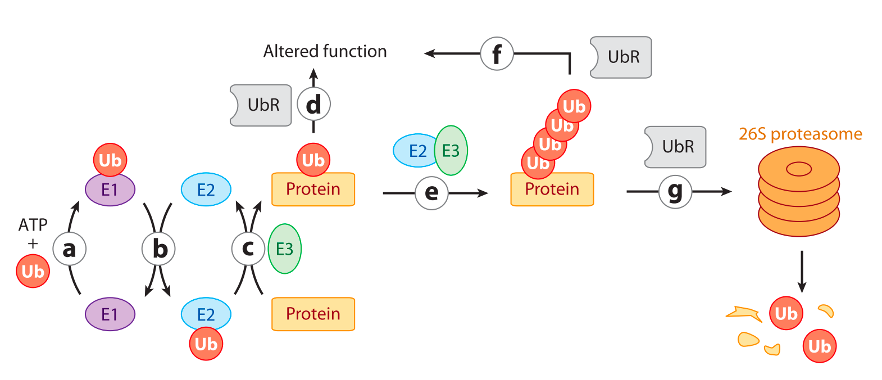
\includegraphics[scale=0.95]{ubiquitination_pathway}
\setlength{\abovecaptionskip}{20pt}
\centering
\mycaption{Title}{Caption}
\label{fig:ubiquitination_pathway}
\end{figure}

A single E1 works with fewer that 40 E2s (in humans), which work with hundreds of E3s. The choice of E2 often determines the type of ubiquitination that occurs. This can be either monoubiquitination, where a single ubiquitin molecule is added to a target lysine, or polyubiquitination, meaning the formation of a ubiquitin chain via lysine molecules on ubiquitin monomers. The functional consequences of ubiquitination are directly related to the type of ubiquitination. Monoubiquitination is associated with modification of protein function. <more>. Depending on the type of linkage, polyubiquitination can also be associated with modification of protein function, but is most commonly associated with proteasome-dependent proteolysis. Each E3 typically interacts with only a small number of E2s, and a small number of substrates. Therefore, by acting as a bridge between a specific E2 and a specific substrate, E3s are responsible for conferring specificity to the ubiquitination reaction.\\

It is thought that many RING domain proteins (if not most) possess E3 ligase activity (Deshais, CHECK), catalysing the transfer of Ub directly from an E2 to a target substrate. RING E3s work by binding to and stabilising the closed conformation of an E2~Ub conjugate. This alters the geometry of the thioester bond between Ub and E2, increasing reactivity towards a substrate lysine residue. At the same time as interacting with the E2, RING E3s bind to a substrate, bringing a specific lysine on the substrate into close proximity of the E2. This then leads to direct transfer of Ub from the E2 to the substrate. Typically, this E3/substrate interaction is via other parts of the E3 protein, rather than the RING domain itself (e.g. TRIMs use C-terminal substrate recognition domains). \\

Alternatively, lysines on the E3 itself can be targeted. Many E3s are known to be autoubiquitinated. In many cases this may be a side effect of E3 activity with no functional role, but in some cases this may serve a purpose. Autoubiquitination of BCA2 has been shown as an elegant mechanism to regulate steady state levels of the protein \citep{Amemiya2008}. As autoubiquitination is competitive with substrate ubiquitination, the protein is able to regulate its own levels according to substrate availability. <Other examples in the review>.\\


\subsubsection{RINGs as dimerisation domains}

Another key function attributed to RING domains is their ability to act as dimerisation domains. Many purified RING domains have been shown to self-associate in crystal structures, forming dimers or higher order oligomers. In most cases, dimerisation is achieved via hydrophobic interactions between short alpha-helical segments at the N and C termini of the core RING domain, which forms a four-helix bundle involving two RING monomers (fig x). This is stabilised by additional contacts in the core RING domain. \\

However, whilst the majority of RING domains are dimeric in crystal structures, the oligomeric state in solution varies dramatically, ranging from entirely monomeric to constitutively dimeric. For example, whereas TRIM32 appears constitutively dimeric in solution \citep{Koliopoulos2016}, TRIM21 exists in a monomer-dimer equilibrium \citep{Dickson2018}, whereas TRIM25, whilst crystalising as a dimer, appears entirely monomeric in solution, only dimerising at very high concentrations \citep{Koliopoulos2016}. <comment on this, related to interface size?, deltaG?>.\\

In many cases the significance of dimerisation is fundamentally linked to the ubiquitination role of RINGs. RING dimerisation stabilises the closed E2-Ub conformation, by allowing each Ub to make simultaneous contacts with two RING domains. In many cases this is essential for ubiquitination activity. Mutations to key hydrophobic residues in the helices flanking the core RING domain disrupt dimerisation and reduce ubiquitination activity. On the other hand, forced dimerisation of RINGs can hyperactivate ubiquitination activity, as has been shown for RNF4 (ref). \\

In the case of RING domains at the weaker end of the dimerisation scale, which exist largely as monomers in isolation, the ability to dimerise may be context specific. RNF4 is largely monomeric at physiological concentrations in vitro, but is able to dimerise upon addition of its substrate. Dual binding of two RNF4 molecules to a single substrate molecule creates a locally high concentration of RNF4 that permits dimerisation \citep{Rojas-Fernandez2014}. <comment on this> Similarly, TRIM25 shows weak dimerisation ability on its own, but is stabilised by binding to an E2. \\

Notably, however, not all RING domains dimerise. Whereas some form higher order structures (e.g. the TRIM19 RING, which forms a ‘torus-shaped’ tetramer in crystal structures), others lack any ability to oligomerise. The TRIM28 RING domain, for example, has a small N-terminal helix, but lacks a C-terminal helix, and forms no dimerisation contacts in crystal structures (ref). The TRIM56 RING domain lacks both helices, and similarly is monomeric in crystal structures (ref). Likewise, the CBL class of RING domains <more>. In the absence of dimerisation, E2~Ub stabilisation often requires additional contacts outside the RING domain. For example, in the CBL class of RING domains, a phosphorylated tyrosine residue outside of the core RING domain interacts with Ub, which synergises with the RING domain to stabilise the E2~Ub in a similar manner to a dimeric RING (Dou).\\

Given the widespread roles of dimerisation <>, it’s not unlikely that RING domains have evolved functions as dimerisation domains in other contexts unrelated to ubiquitination….\\


\subsubsection{Discussion}

%%%%%%%%%%%%%%%%%%%%%%%%%%%%%%%%%%%%%%%%%%%%%%%%%%%%%%%%%%
\clearpage
\section{A pipeline for quantification of membrane and cytoplasmic protein concentrations}

Intro to section

\subsection{Autofluorescence correction}

Note: this section has been adapted from \textcite{Rodrigues2022}, and describes work performed in conjunction with Nelio Rodrigues.

\subsubsection{Autofluorescence in C elegans}

One major barrier in quantitative experiments using C elegans is autofluorescence. Whilst usually minor in red channels excited with xxx wavelengths, autofluorescence is particularly prominent in channels excited with blue wavelengths which are commonly used to image green fluorophores. When using endogenously tagged proteins, which are often expressed at low levels, this contribution is often be a significant fraction of the total signal, and can therefore significantly obscure the true signal that one is interested in. This might pose particular problems for quantitative experiments, where the absolute signal levels may be important.\\

We can observe this problem by imaging untagged control embryos. As shown in (fig x), a significant amount signal is collected in the GFP channel, which varies both spatially within the image, and between different images. By comparison, total signal in embryos endogenously tagged with LGL GFP is also highly variable, and only marginally higher than N2s, suggesting that a significant fraction of the total signal observed in these cells is autofluorescence, and that the intra-embryo signal variation is largely due to variable autofluorescence. Despite being enriched on the posterior cortex, which is easily visible in cells with overexpressed LGL (ref), this is difficult to visualise here as a result of autofluorescence. Therefore, if we want to accurately visualise, and indeed quantify, protein levels and distributions, we need a method that can locally correct AF on a pixel-by-pixel basis.\\

% figure demonstrating autofluorescence

One approach that has been used for this is spectral imaging. Typically used to separate overlapping fluorophore signals based on spectral characteristics, this approach can also be used to separate out autofluorescence by treating it much like a fluorophore with its own spectral characteristics. Whilst often effective, these techniques require specialised instruments and analysis tools and cannot be performed on standard confocal microscopes.\\

However, simpler approaches have been used. By exploiting the fact that autofluorescence can often be described as a single component, with an emission spectrum much broader than GFP, one can find an emission wavelength (usually red) that is specific for autofluorescence, and use this channel to infer the amount of autofluorescence in the sample. This can then be subtracted away from the fluorophore channel, giving a ‘clean’ readout of fluorophore signal. In comparison to full spectral imaging, this method can be carried out with standard light sources and emission filters, and therefore can be easily implemented into existing workflows.\\

Inspired by this work, we aimed to implement, and assess the applicability of such a method to images of C elegans zygotes. In doing so, we have put together a robust and easily-implementable workflow which we’ve termed SAIBR: Spectral Autofluorescence Image correction by regression.\\


\subsubsection{SAIBR: a simplified method for autofluorescence correction based on dual emission imaging}


At minimum, autofluorescence correction relies on the ability to find a reporter channel that is free of GFP signal, but rich in autofluorescence, such that this channel can be used an independent readout of autofluorescence in the sample. Full spectral analysis performed by Nelio Rodrigues (not shown here), shows that red shifted emission filters, which are commonly used to image red fluorescent proteins, meet such a requirement.\\

Furthermore, by imaging untagged embryos with both the standard GFP channel and the AF channel, we find a strong linear correlation between pixel data from the two channels. Whilst raw pixel values do not correlate well, as these are dominated by noise, we can get a strong correlation by first applying a Gaussian filter to suppress this noise (fig x). We found that this relationship is consistent between embryos (fig x b, c). Furthermore, we found a near identical relationship when plotting the mean intensity values of individual embryos, suggesting that the same relationship can account for both intra- and inter-embryo AF variation. \\

\begin{figure}[!h]
\includegraphics[scale=0.95]{saibr_n2_correlation}
\setlength{\abovecaptionskip}{20pt}
\centering
\mycaption{Title}{Caption}
\label{fig:saibr_n2_correlation}
\end{figure}


Together, this implies that taking an autofluorescence channel image is sufficient to accurately predict the level of autofluorescence in the GFP channel. To quantify the necessary inter-channel conversion factor, I performed linear regression, using an ordinary least squares method, on Gaussian-filtered pixel values pooled from multiple untagged embryos. Then, to perform correction on images containing fluorophore, we just need to capture an autofluorescence channel image, alongside the GFP channel image, rescale the image according to this predefined relationship, and then subtract this away from the GFP channel image.\\


\subsubsection{Assessing performance on images of PAR proteins}

To assess the effectiveness of SAIBR, and it’s utility in the analysis of PAR proteins, I applied it to a range of images of unlabelled and GFP-labelled embryos. As expected, applying SAIBR to images of unlabelled cells reduced fluorescence from across the cell to zero, with no visible structures remaining. This is a good validation of the method, and suggests that it can properly account for all of the autofluorescence in the cell. \\

As already shown, images of LGL are dominated by autofluorescence, and so SAIBR was expected to be particularly useful. As shown in fig x, SAIBR strongly reduces signal within the cell, and improves contrast at the posterior cortex, allowing us to better resolve cortical enrichment at the posterior. Improvements are similar for PAR-3. In addition to improvements at the cortex, we see that SAIBR can suppress the local fluorescence minimum at the cell centre caused by lower AF at the pronuclei. For PAR-6 the improvements are qualitatively less striking, due to a higher ratio of fluorophore signal to autofluorescence, but nonetheless quantitatively important.\\

\begin{figure}[!h]
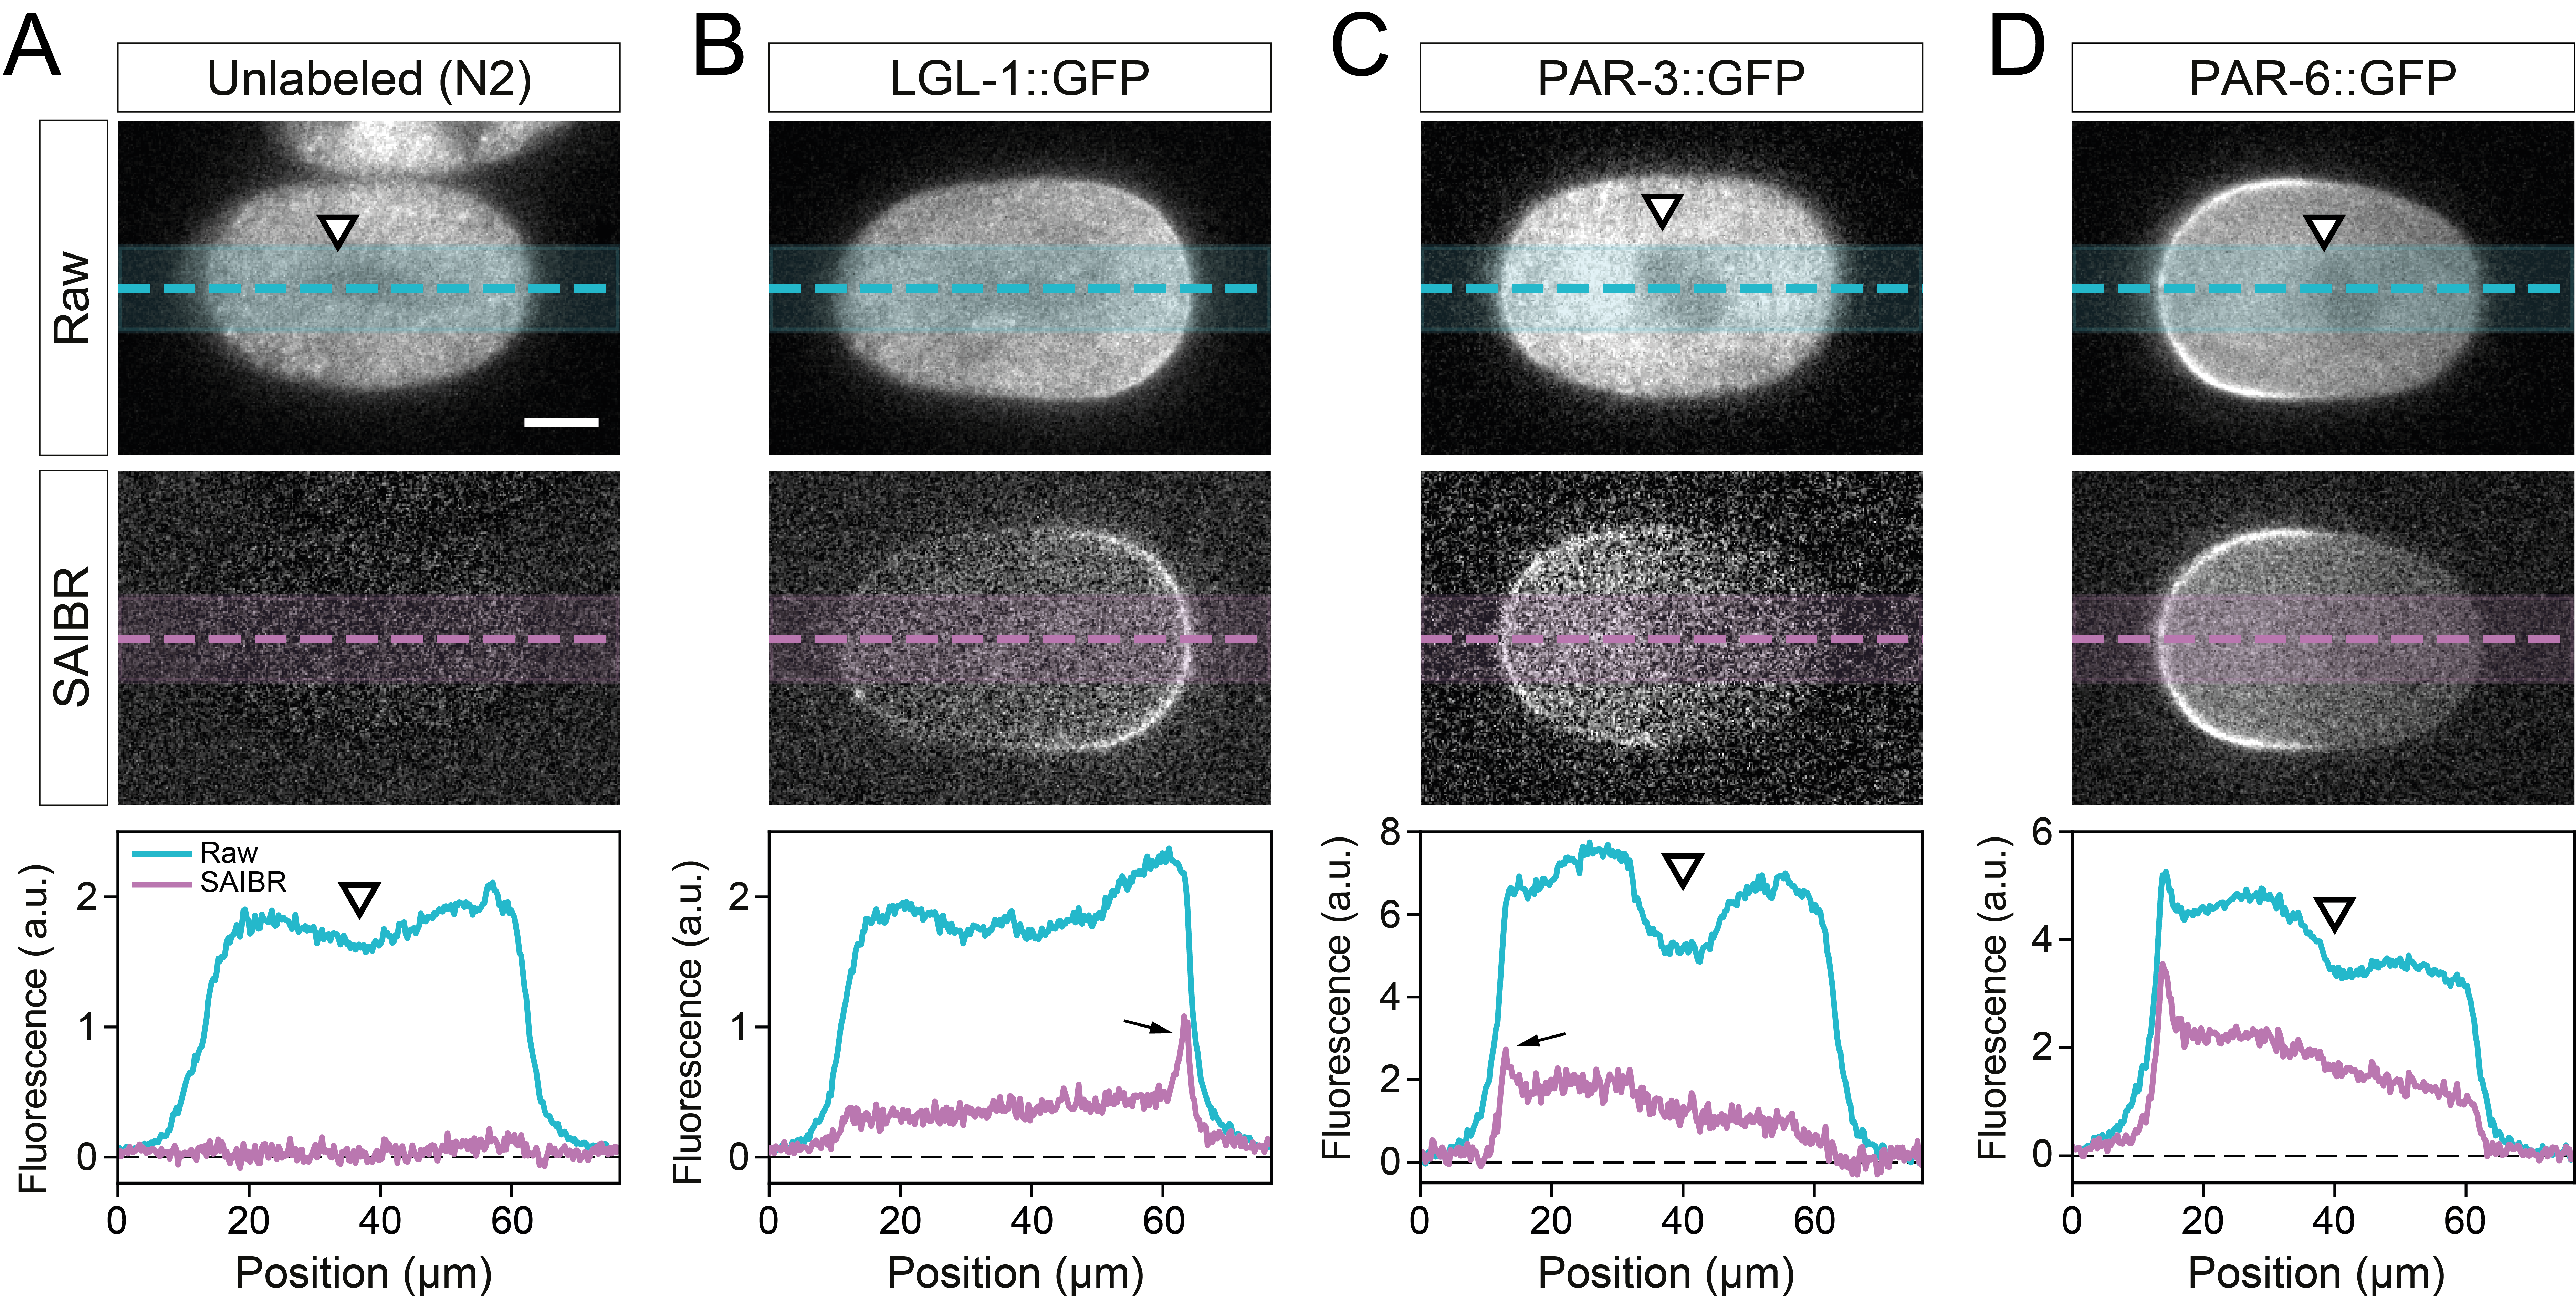
\includegraphics[scale=0.9]{saibr_spatial_correction}
\setlength{\abovecaptionskip}{20pt}
\centering
\mycaption{Title}{Caption}
\label{fig:saibr_spatial_correction}
\end{figure}

As shown in fig x, SAIBR has a strong impact on the shape of intensity profiles taken across the cortex within each polarity domain, in all cases showing a clearer peak and suppression of signal at the internal portion of the curves. This has particular importance for quantitative studies as, as described in the next section, the shape of cross-cortex profiles are often used to quantitatively analyse membrane concentrations and/or membrane affinities. For example, a profile with a central peak that is much higher than the internal cytoplasmic plateau clearly implies that the protein is binding to the membrane with a high affinity. We can see from the SAIBR corrected profiles that, of the three proteins shown here, LGL has the strongest membrane affinity (highest enrichment at the cortex compared to its cytoplasmic level), followed by PAR-6, followed by PAR-3. If we look at the profiles pre-correction, however, this isn't so clearly apparent. One may have some success by simply subtracting an equivalent profile taken from untagged N2s. However, such a method fails to account for the fact that much of variation between embryos is down to autofluorescence, and is thus unsuitable for any study where inter-embryo variation is important. In the case of LGL this would also clearly result in negative values at the cytoplasmic portion of the curve for some embryos.\\

% more here about membrane affinity, on rates, off rates


\begin{figure}[!h]
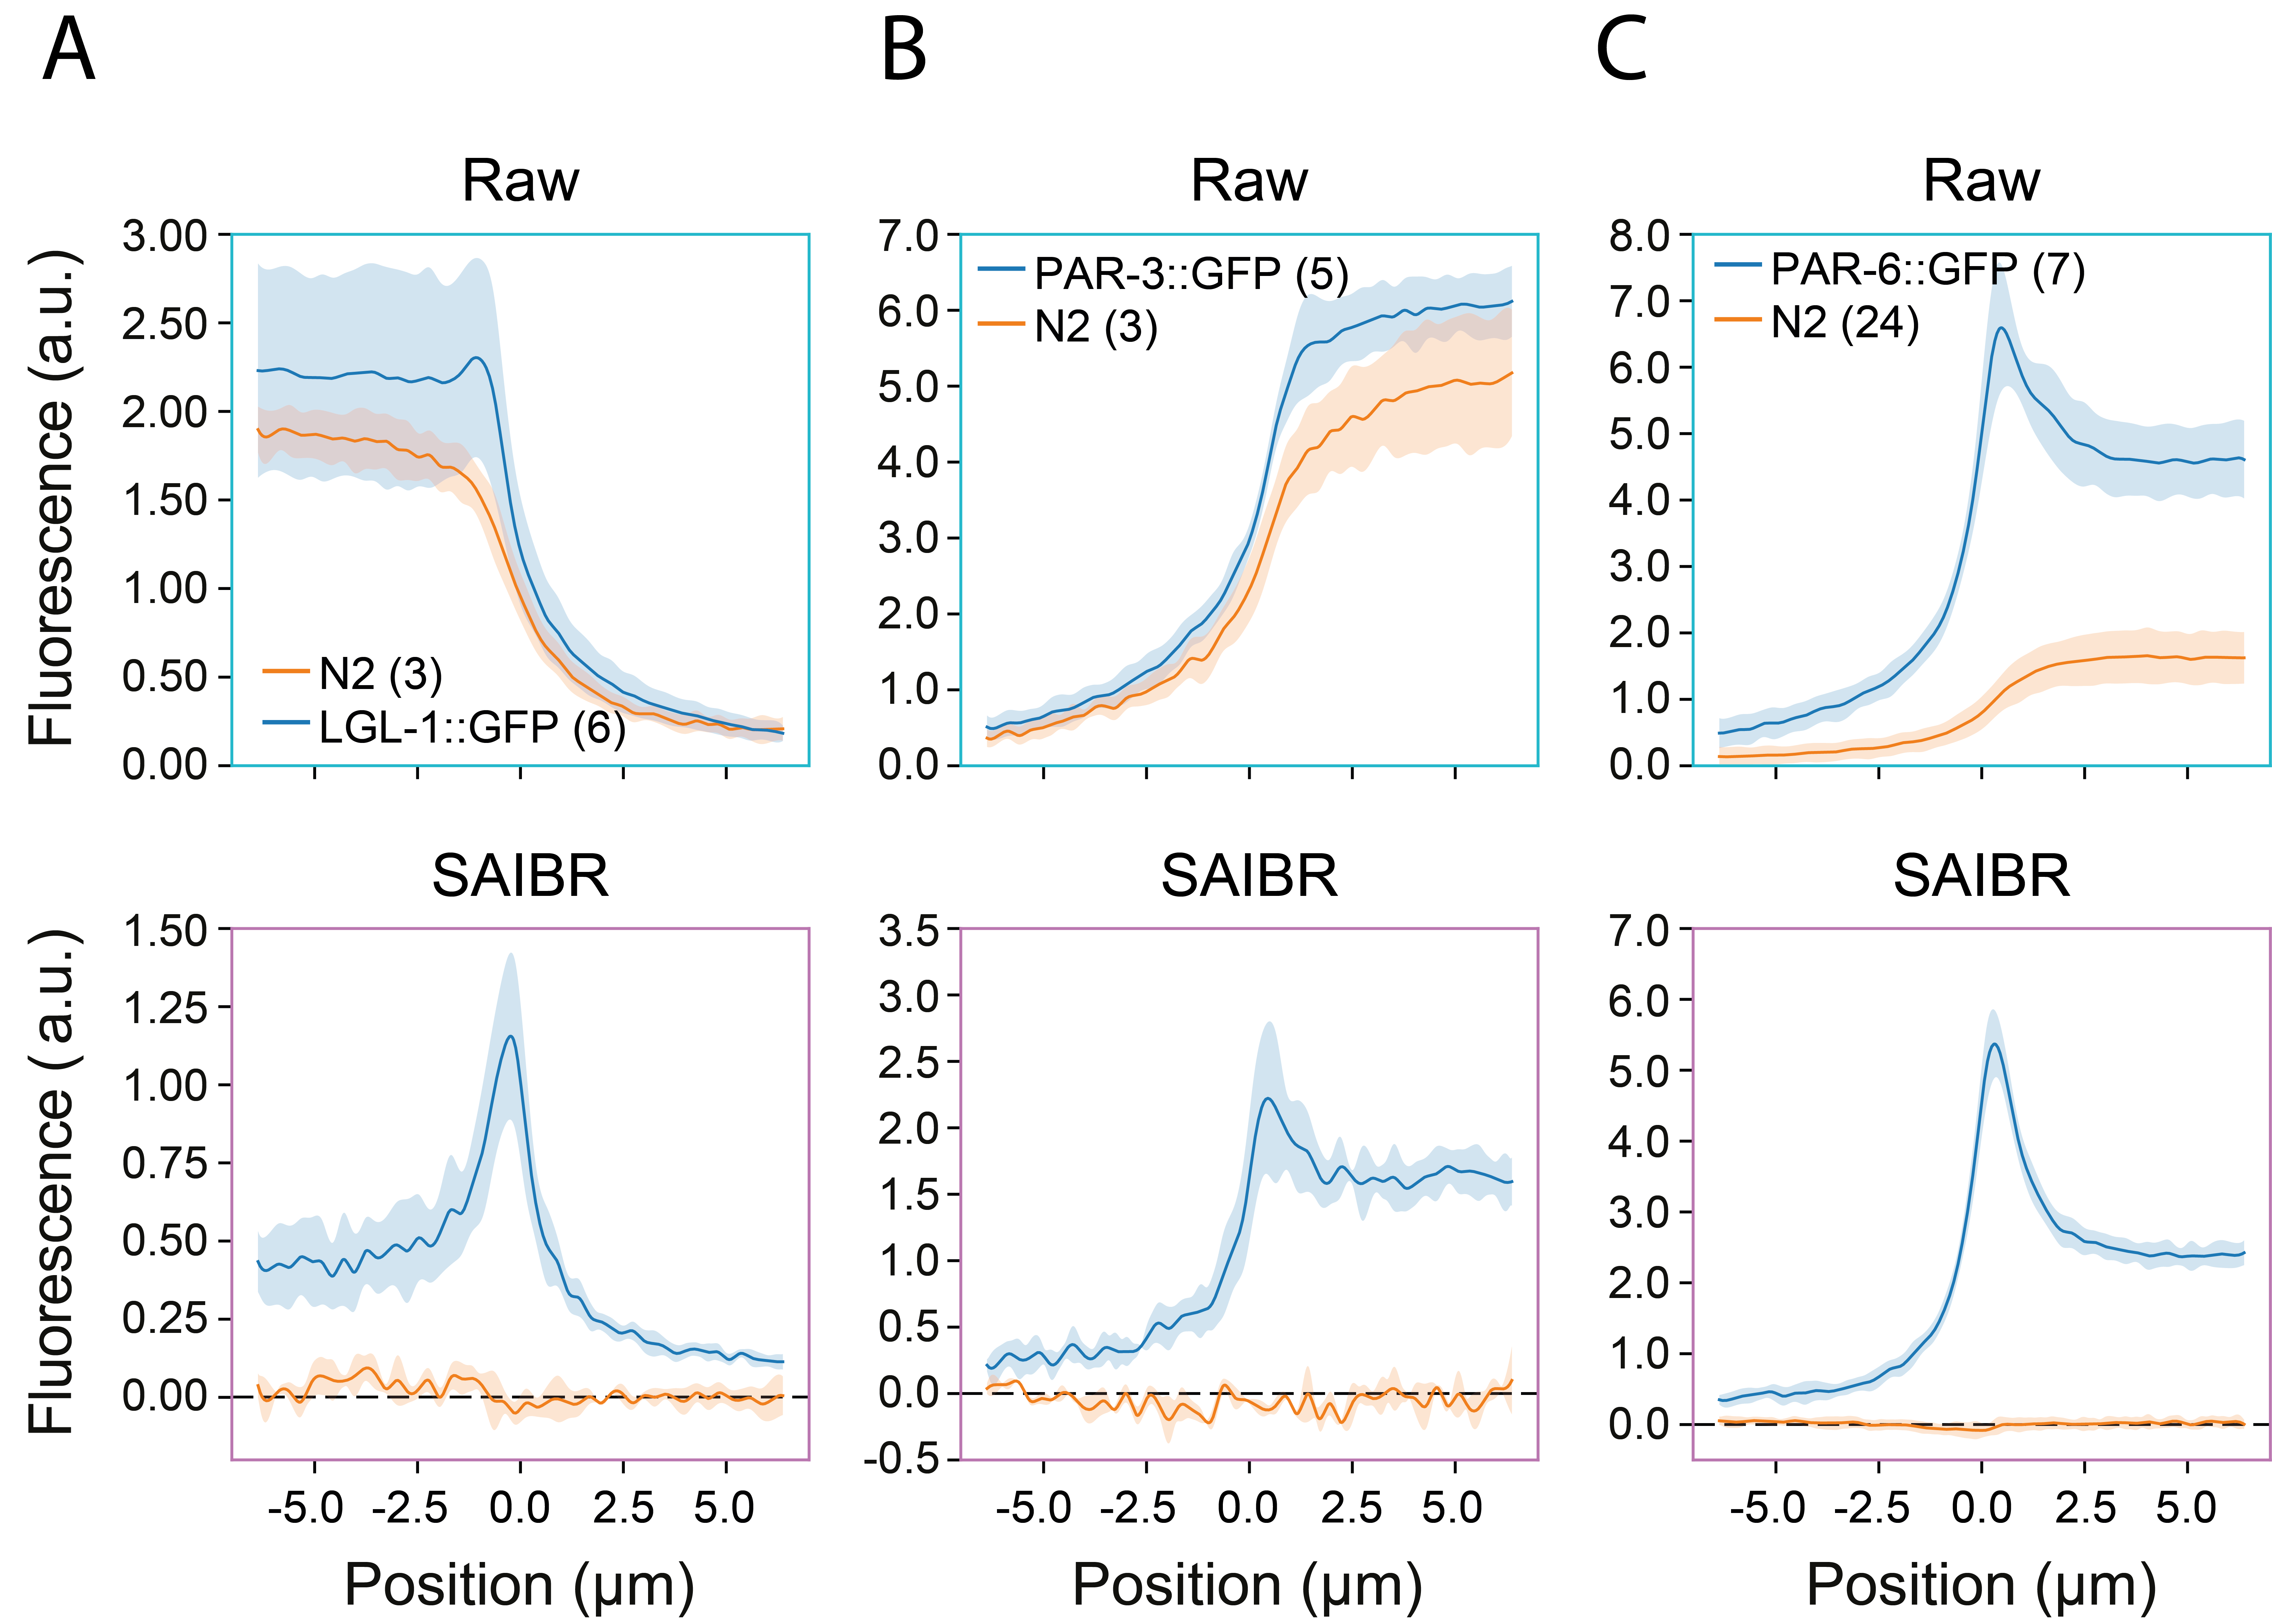
\includegraphics[scale=1]{saibr_membrane_profiles}
\setlength{\abovecaptionskip}{20pt}
\centering
\mycaption{Title}{Caption}
\label{fig:saibr_membrane_profiles}
\end{figure}

\subsubsection{Extending SAIBR to dual-labelled C elegans embryos}

As SAIBR relies on a red shifted emission channel, complications can arise when there is a red fluorophore present. As red fluorophores are usually weakly excited by blue lasers, they will contribute additional signal to the AF channel, which may lead to overestimation, and therefore oversubtraction, of autofluorescence if not accounted for. If RFP levels are low, this effect may be small and can be ignored. However, if RFP levels are high, this bleedthrough effect can be significant. This can be demonstrated by observing the inter-channel relationship in control embryos tagged with a red fluorophore (fig x). We find that, when an RFP is present, this relationship deviates significantly from the typical relationship observed in N2s, in direct proportion to local RFP levels (fig x inset). As this relationship is linear, autofluorescence in the GFP channel can now be described as a linear function of both the AF and the RFP channels. Plotting the pixel data in three dimensions shows that the data can be successfully fit to a plane, by performing multiple linear regression (fig x). \\


\begin{figure}[!h]
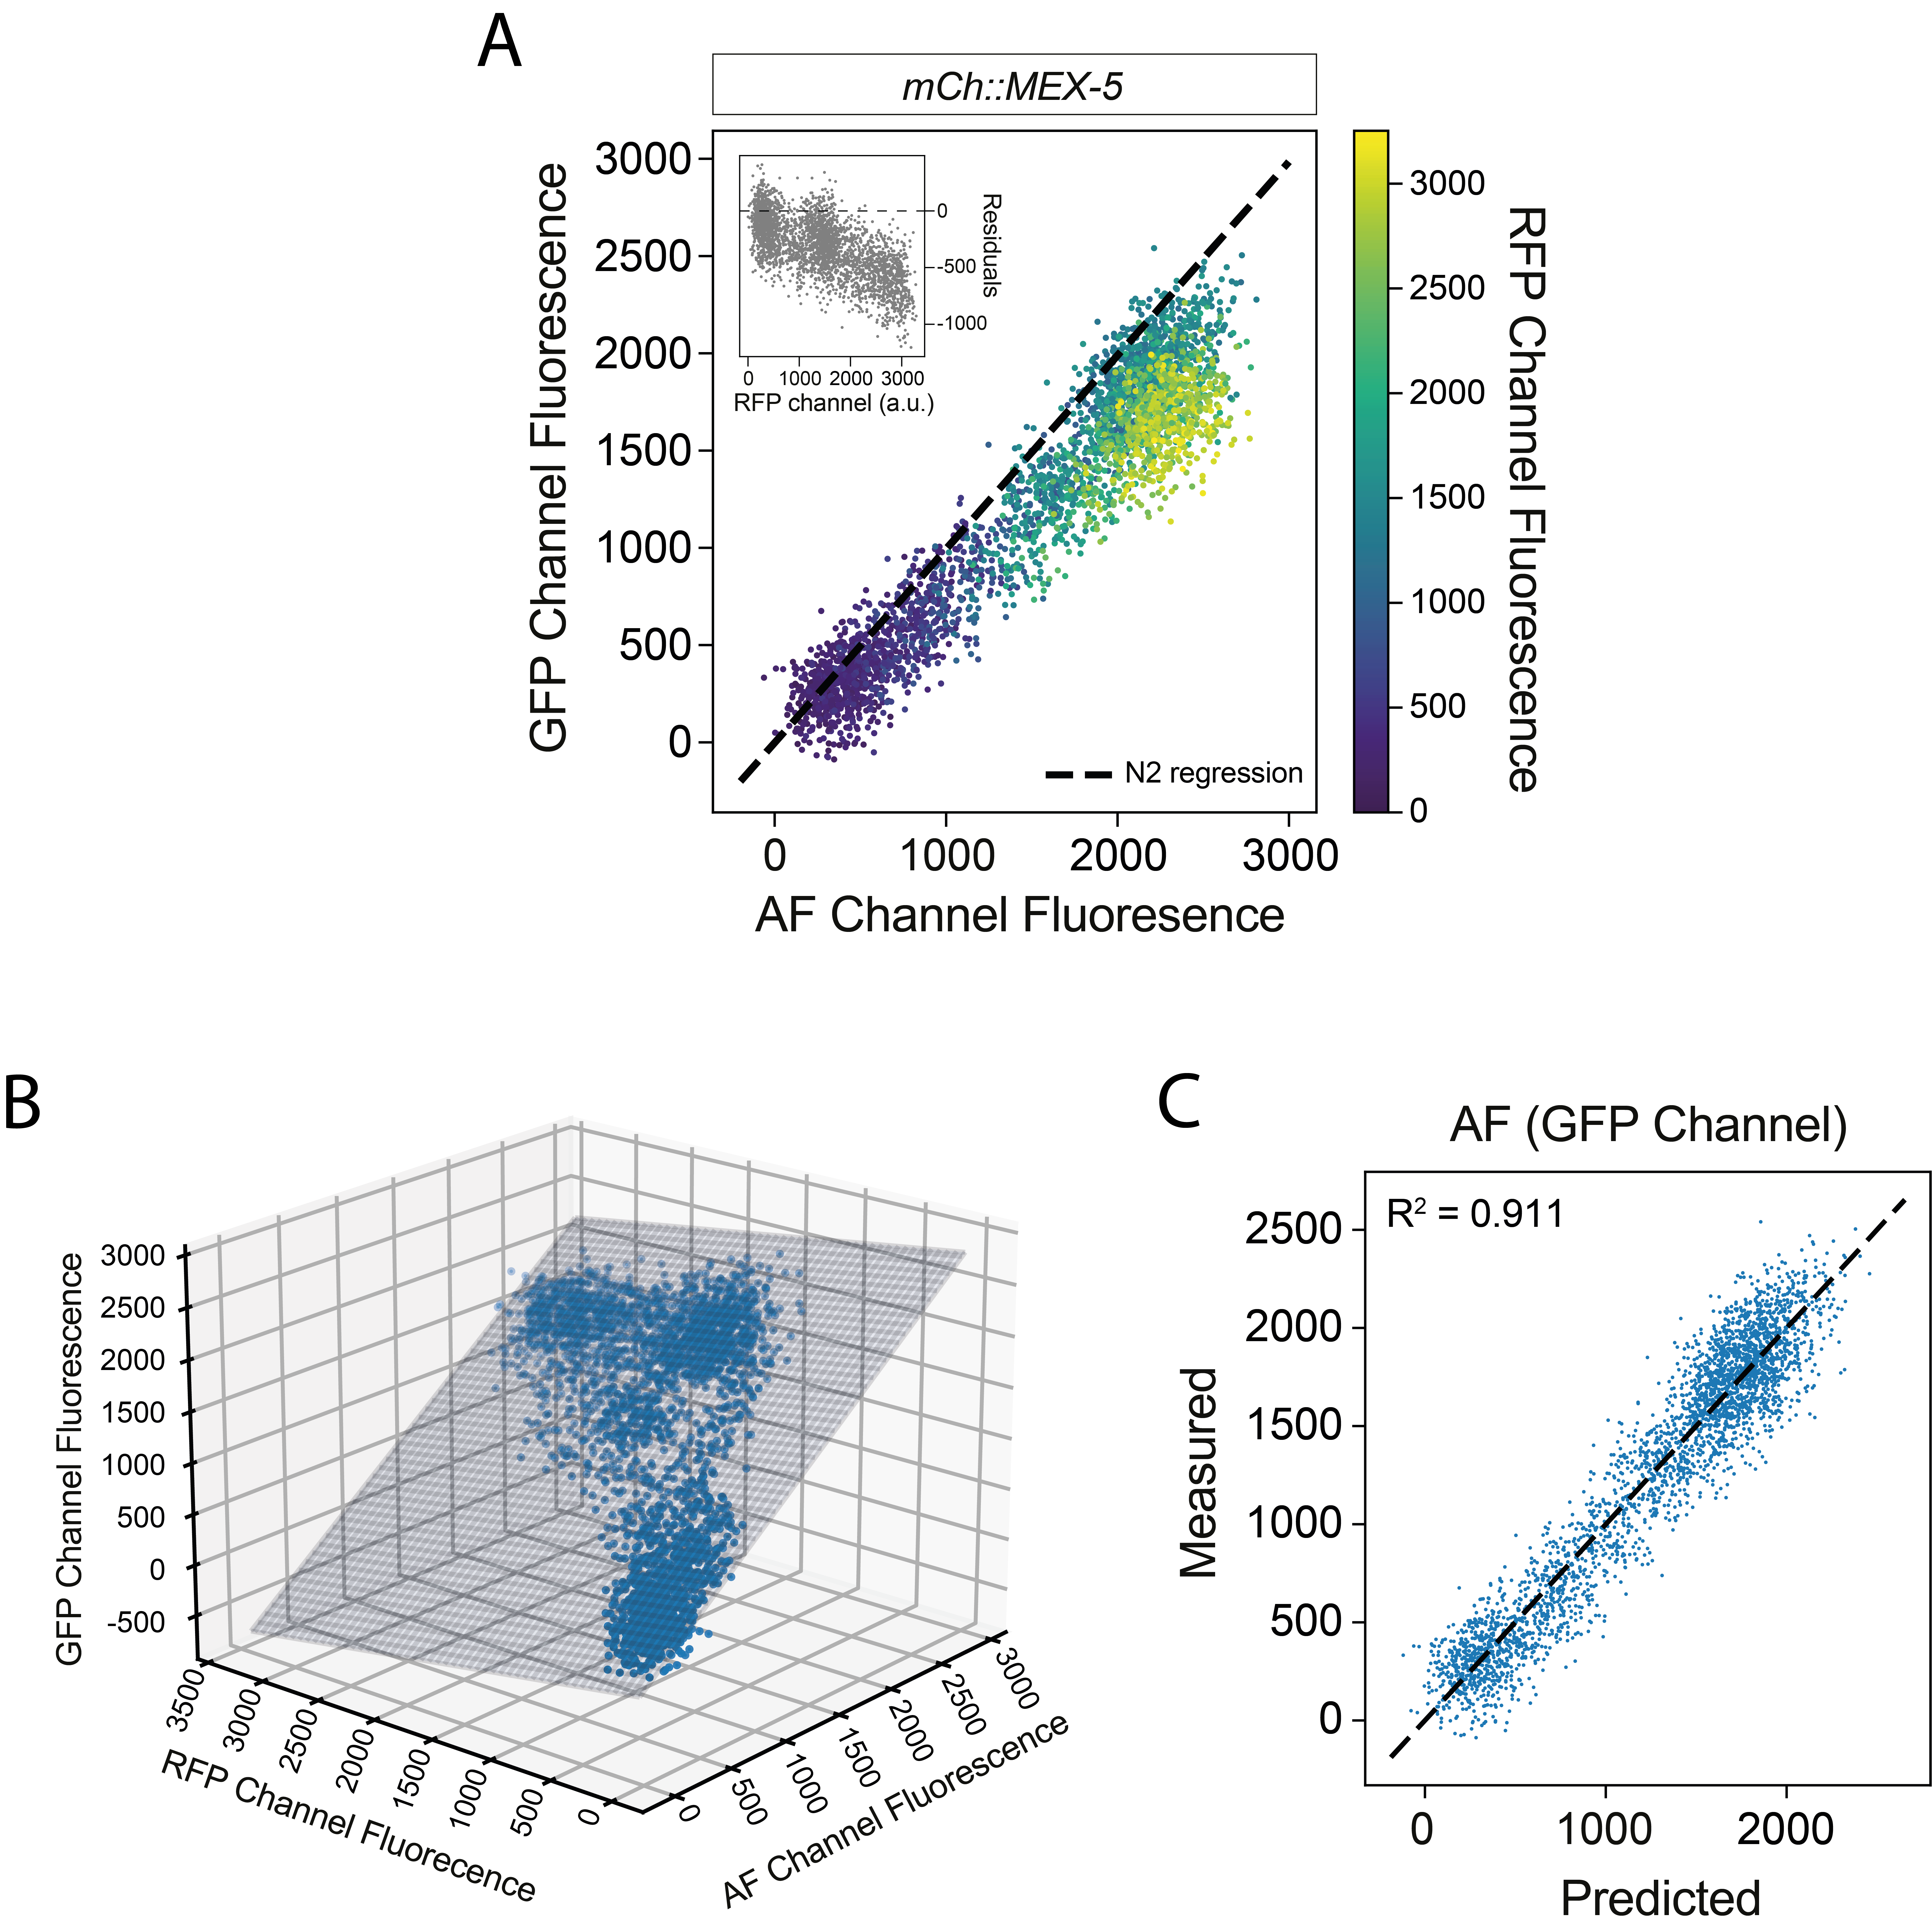
\includegraphics[scale=1]{saibr_3channel_correlation}
\setlength{\abovecaptionskip}{20pt}
\centering
\mycaption{Title}{Caption}
\label{fig:saibr_3channel_correlation}
\end{figure}

Then, to perform correction on images containing fluorophore, we just need to capture all three channels, calculate autofluorescence using the three-channel regression relationship obtained from the appropriate RFP tagged single line, and then subtract this away from the GFP channel image. This is demonstrated in figure x, for embryos expressing both PAR-6 GFP and MEX5 mCherry, or just MEX5 cherry. Whereas 2-channel SAIBR results in oversubtraction of autofluorescence (particularly visible in the MEX5 cherry single line), this is eliminated when using 3-channel SAIBR.\\

\begin{figure}[!h]
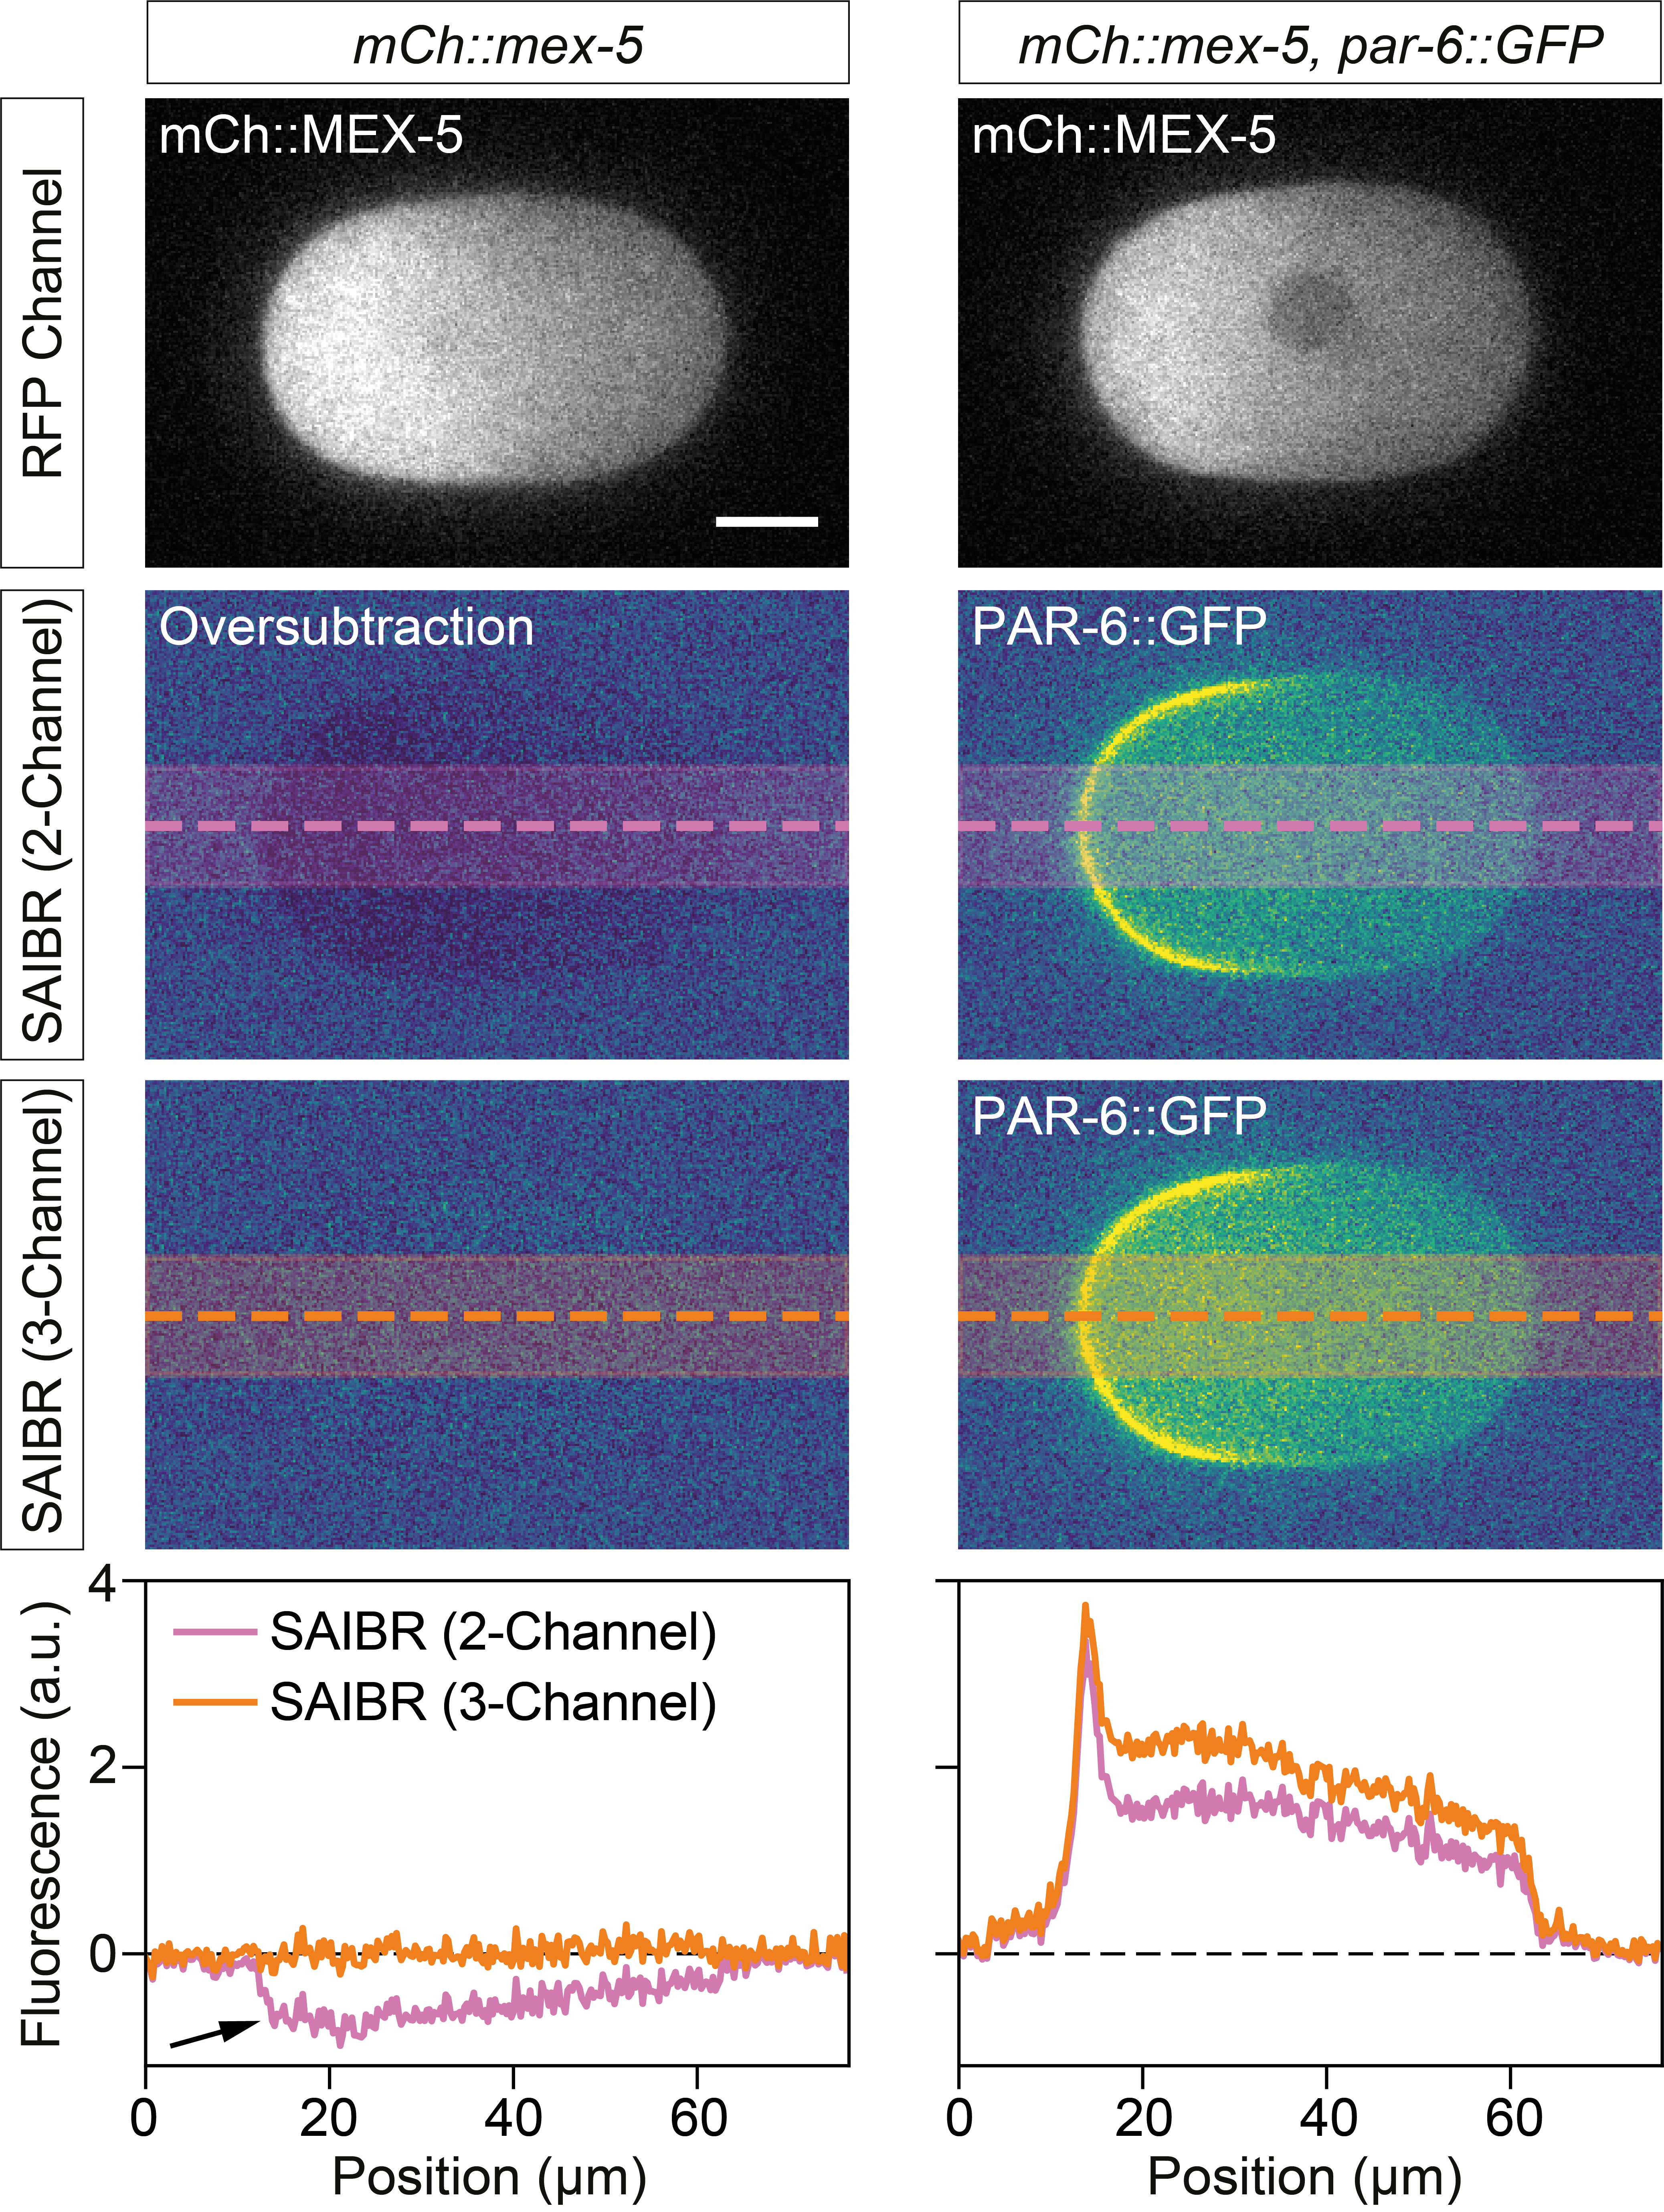
\includegraphics[scale=1]{saibr_3channel_correction}
\setlength{\abovecaptionskip}{20pt}
\centering
\mycaption{Title}{Caption}
\label{fig:saibr_3channel_correction}
\end{figure}


\subsubsection{Discussion}

In summary, I have demonstrated that a simple protocol, which we’ve termed SAIBR, can be used to successfully correct autofluorescence in images of C elegans zygotes. The improvements are particularly striking for images of fusion proteins with low levels of expression, such as LGL, but even when expression levels are higher, such as PAR-2, AF correction will prove important for quantitative analysis, as discussed in the next section. \\

The simplicity of the method means that it can be easily incorporated into existing workflows, and should be applicable to a variety of imaging platforms. In the full study, we showed that the method is equally successful on both spinning-disk confocal and wide field instruments. \\

Whilst designed with C elegans embryos in mind, the method isn't specific to this system, and could be applied to a number of other model systems in which autofluorescence is a problem. In the full study, we have shown that the method works successfully in C elegans larvae, as well as other model organisms such as starfish and yeast. That said, the method isn’t guaranteed to perform well in all cases. If samples contain multiple, independently varying sources of autoflourescence, then SAIBR may face problems as a single autofluorescence reporter channel cannot account for this. However, much like how we can tackle red fluorophores, we have found that in some cases this can be solved simply by adding one extra reporter channel. Inevitably, though, such an approach may not be compatible with dual-colour imaging. \\

Whilst the analysis steps are relatively straightforward, implementing the computational workflow may still be a barrier to adoption for some. Therefore, to make the protocol accessible, I have put together a simple GUI-based FIJI plugin which can carry out all the analysis steps in a few simple steps. This can be found here: \url{https://github.com/tsmbland/saibr_fiji_plugin}. \\

The method comes with a few tradeoffs, which will vary in significance depending on the particular study. One issue is that, as the method combines pixel noise from multiple images, corrected images can in some cases be quite noisy, particularly where weak imaging conditions are used. It also requires capturing two emission channels for each image, which doubles sample illumination times and potential phototoxicity, which may be an issue for long timelapses. Additionally, if samples display rapid motion, then the time lag between taking these two channels may lead to pixel mismatches, which could introduce artefacts. These last points could be fixed by using an imaging setup that allows for dual capture of multiple emission bands. However, for this particular study, none of these issues will be of major significance. \\


\clearpage
\subsection{Extracting membrane and cytoplasmic signal components}

% intro to section

\subsubsection{An overview of existing methods}

A number of methods have been implemented aiming to quantify cortical protein amounts in C elegans embryos. A typical approach to quantify membrane concentrations is to find the region of the image representing the cortex (either by manual or computational segmentation) and take a coarse measure of pixel values within this region (fig x). Such an approach was used by Goehring, who manually segmented the embryo cortex, computationally straightened a region around the circumference of the cell, and summed the highest intensity group of pixels at each cortical cross section. Hubatsch used a similar approach, but replaced manual segmentation with an automated computational pipeline. Similarly, \textcite{Zhang2017} used an elaborate computational protocol to segment images, and defined cortical concentrations around the cell as the average signal intensity within a region representing the cortex.\\

% figure: intensity based vs fitting procedures

A main disadvantage of these methods is that, as the cortex is immediately apposed the cytoplasm, pixel values at the cortex will inevitable contain a contribution from cytoplasmic fluorophore signal (and, indeed, cytoplasmic autofluorescence as none of these methods (?) have employed spatial autofluorescence correction). This means that measurements of membrane concentration will sensitive to changes in cytoplasmic concentrations, and means that these methods fail to achieve an accurate zero (a positive signal will always register, even if there is nothing on the membrane). Typically, attempts are made to overcome this latter point by normalising concentrations and/or subtracting away a local or global estimate of the background signal, but this is often difficult and inaccurate.\\

More advanced methods have aimed to overcome this problem by building models to describe the expected shape of individual cross-cortex profiles, based on summed contributions of cytoplasmic and membrane signal. Membrane and cytoplasmic concentrations can then be extracted by fitting measured profiles to this model, and extracting the relevant parameters describing the amplitudes of the two signal components (fig x). Such an approach was used by Gross, who described the cross-cortex profile at each point around the circumference of the embryo as the sum of a Gaussian and an error function contribution, representing the expected form of a point (cortex) or step-function (cytoplasm) convolved with a Gaussian-like point spread function in 1D. The model also includes a parameter describing the position of the cortex, which can be optimised to align the model to the profile, eliminating the need for accurate prior segmentation. A similar approach was previously used in \textcite{Blanchoud2015} (although with a slightly different description of cytoplasmic signal).\\

\subsubsection{Accounting for out-of-focus scatter}

Whilst these methods have been effectively deployed, and are good at capturing a proper zero baseline, their accuracy is inevitably limited by the accuracy of the underlying models. For many imaging set-ups, the assumption that cytoplasmic and membrane contributions can be described by such simple mathematical functions may in fact be far from the truth. This was demonstrated by for C elegans embryos by Reich (cite thesis), who quantitatively analysed cross-cortex signal in cells containing only cytoplasmic protein, finding that (under imaging conditions similar to those used in this study) the shape of this profile deviates significantly from the expected error-function shape. I have also performed similar analysis here...\\

% * can be seen in figure A.3 of Jake’s thesis, although it’s worth noting that the original study didn’t use spatial autofluorescence correction, so there may be some artefacts relating to this

% description of cytbg figure

% cytbg figure

The main reason for this is likely due to scattering and diffraction of light from planes above and below the imaging plane, combined with a curved geometry in the z-dimension (fig x). Scatter, which is a common issue in images of biological samples, causes a broadening of light in three dimensions as it passes through regions of heterogeneous refractive index. This occurs within the (xy) plane of an image, but is typically far more significant in the z-axis. Whilst confocal microscopes are designed to only capture light from a single plane, they illuminate the whole sample, so will capture any emitted light from other planes that scatters into the focal plane. This means that pixel intensities within the focal plane will be affected not only by structures within that plane but also structures above and below.\\


\begin{figure}[!h]
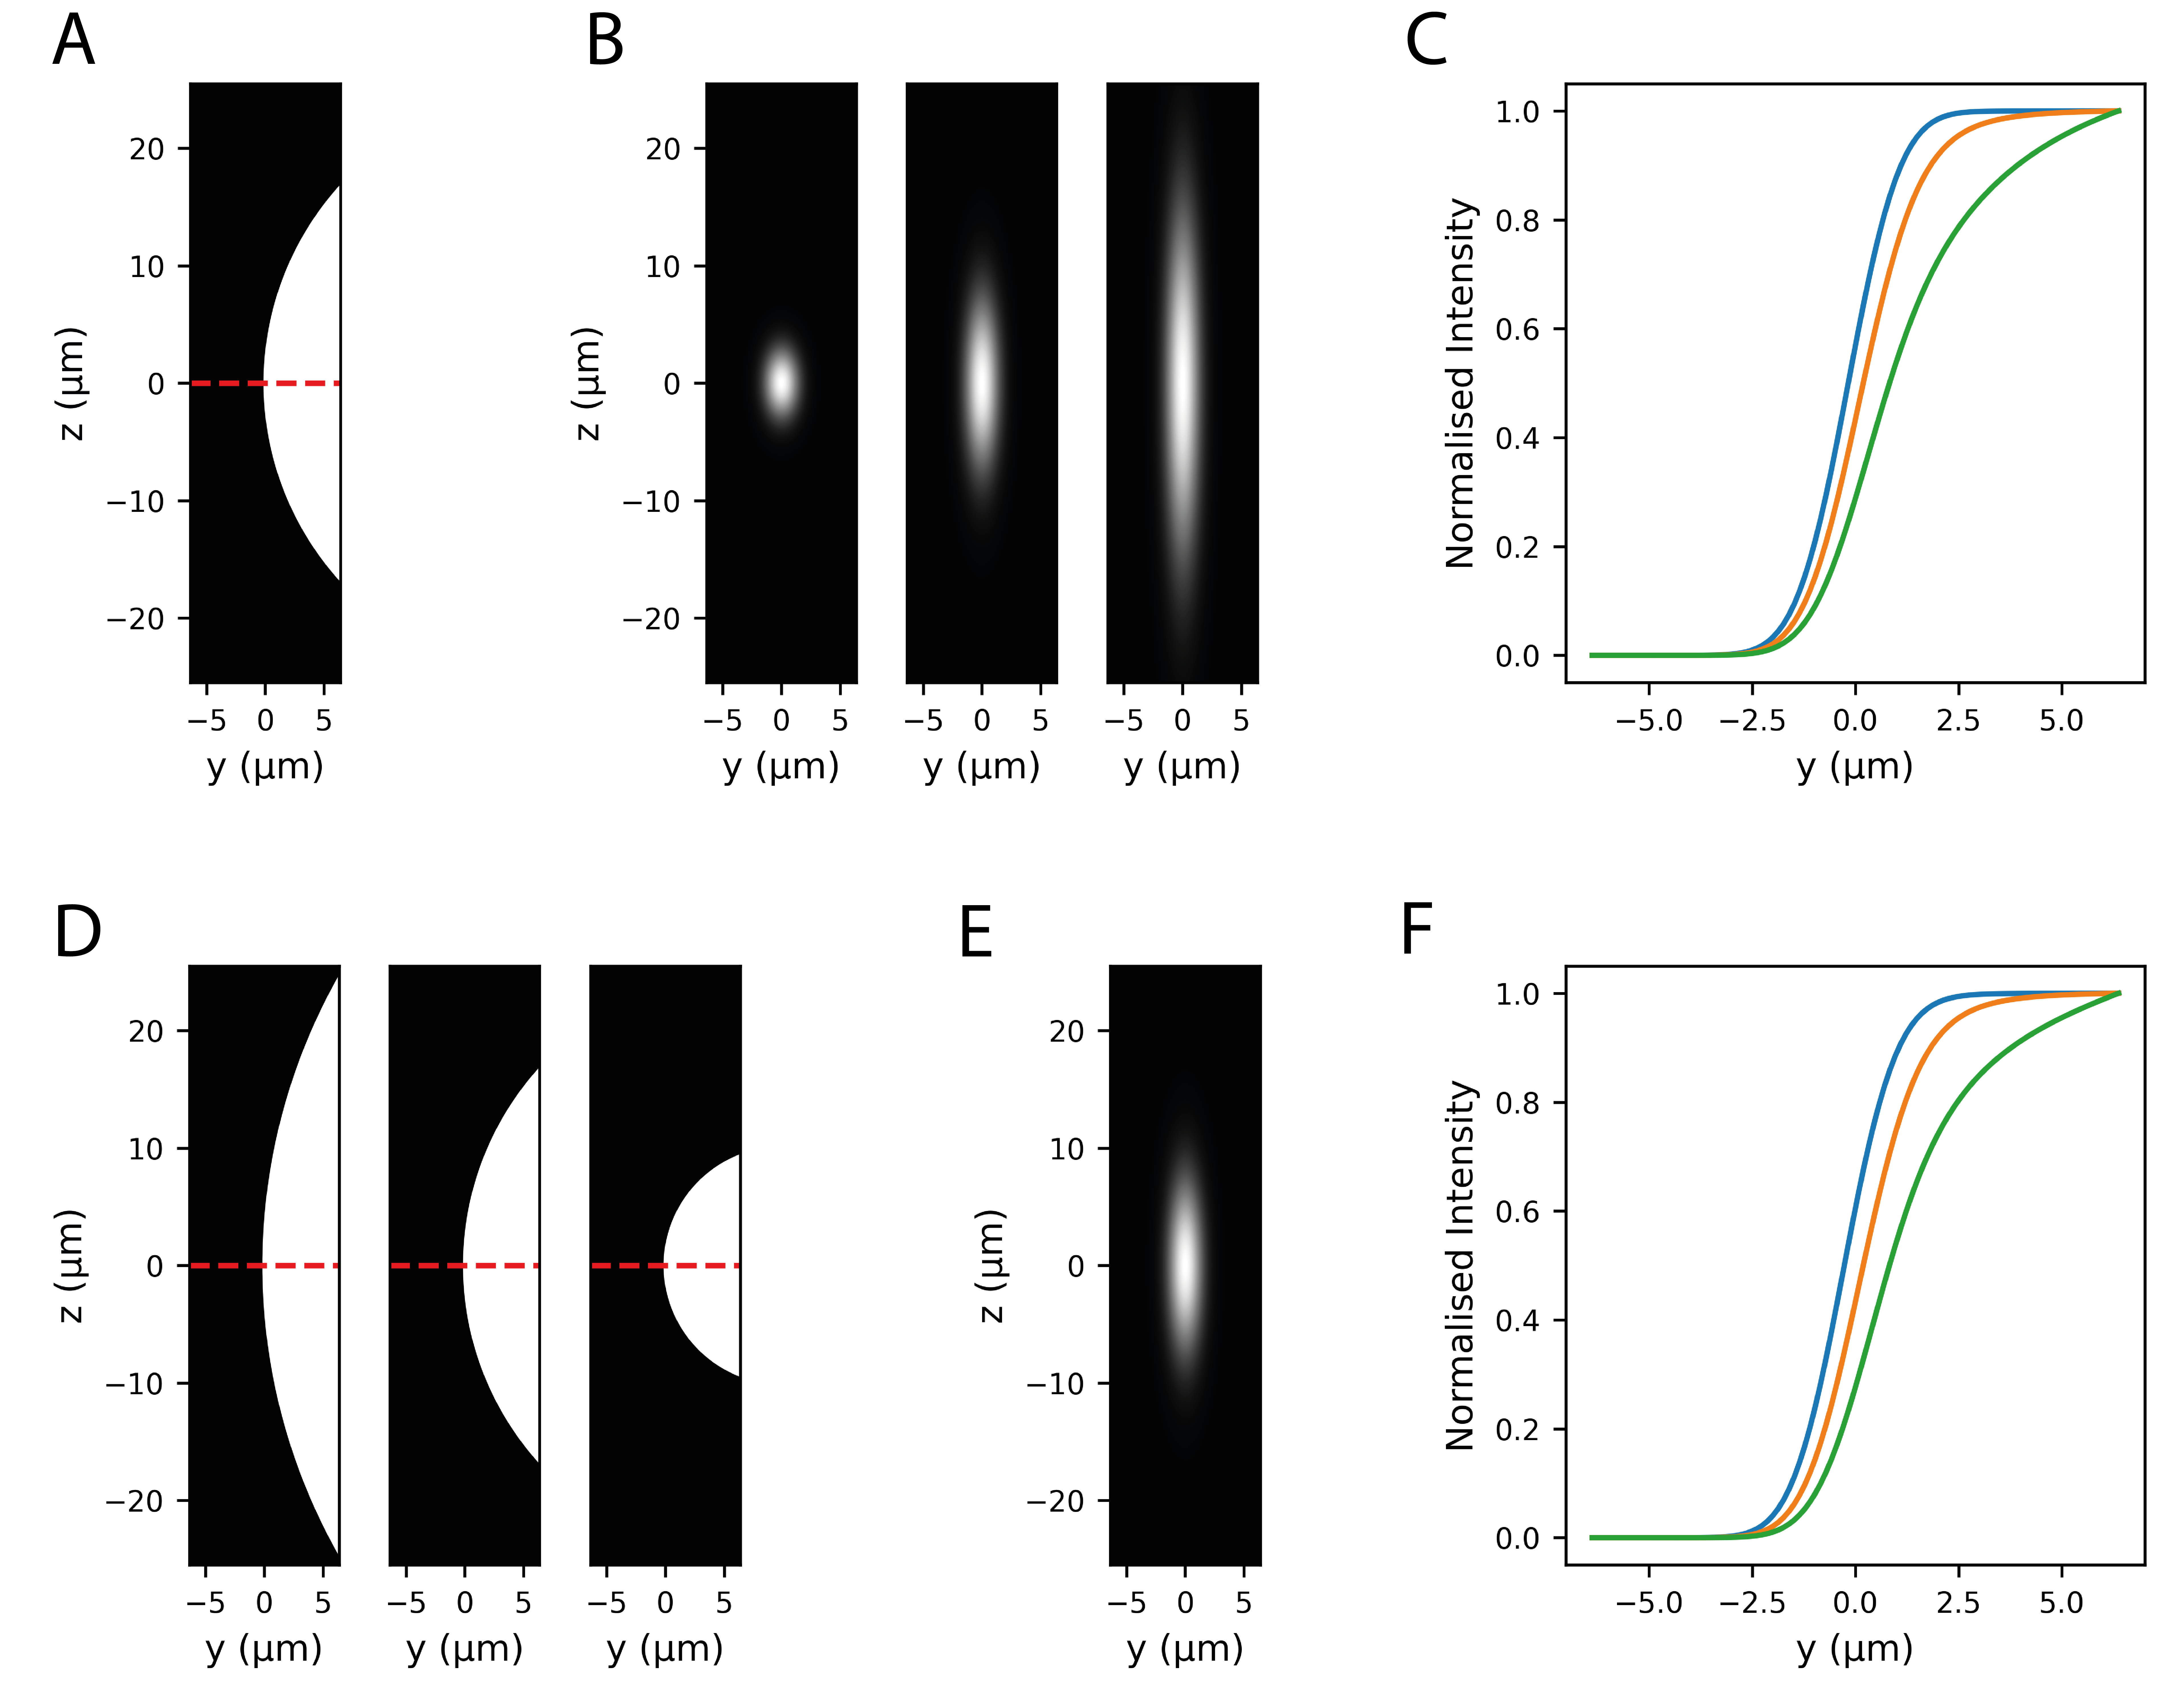
\includegraphics[scale=0.9]{memquant_cyt_psf}
\setlength{\abovecaptionskip}{20pt}
\centering
\mycaption{Title}{Caption}
\label{fig:memquant_cyt_psf}
\end{figure}

It is likely that a similar problem applies in the case of membrane protein (fig x). Specifically, this analysis shows that out of focus cortical signal might expect to lead to a shape resembling an asymmetric Gaussian, with higher signal on the inside than the outside. In fact, this phenomenon can be easily observed just by looking at images of polarised PAR proteins (<reference earlier image>), where out-of-focus cortical signal can create the illusion of a strong cytoplasmic gradient (by comparison, two-photon images of PAR-2, which aim to eliminate out of focus light, show a completely flat cytoplasm \citep{Petrasek2008}, which is expected for most PAR proteins based on fast measured diffusion rates). Whilst in some cases this may be of little concern, this might be particularly problematic if accurate cytoplasmic quantification is required. Without accurate cytoplasmic concentration, measures of membrane to cytoplasmic ratios, which are often used as a proxy for membrane affinity, may be wildly off. This will prove significant for much of the analysis in this study.\\

\begin{figure}[!h]
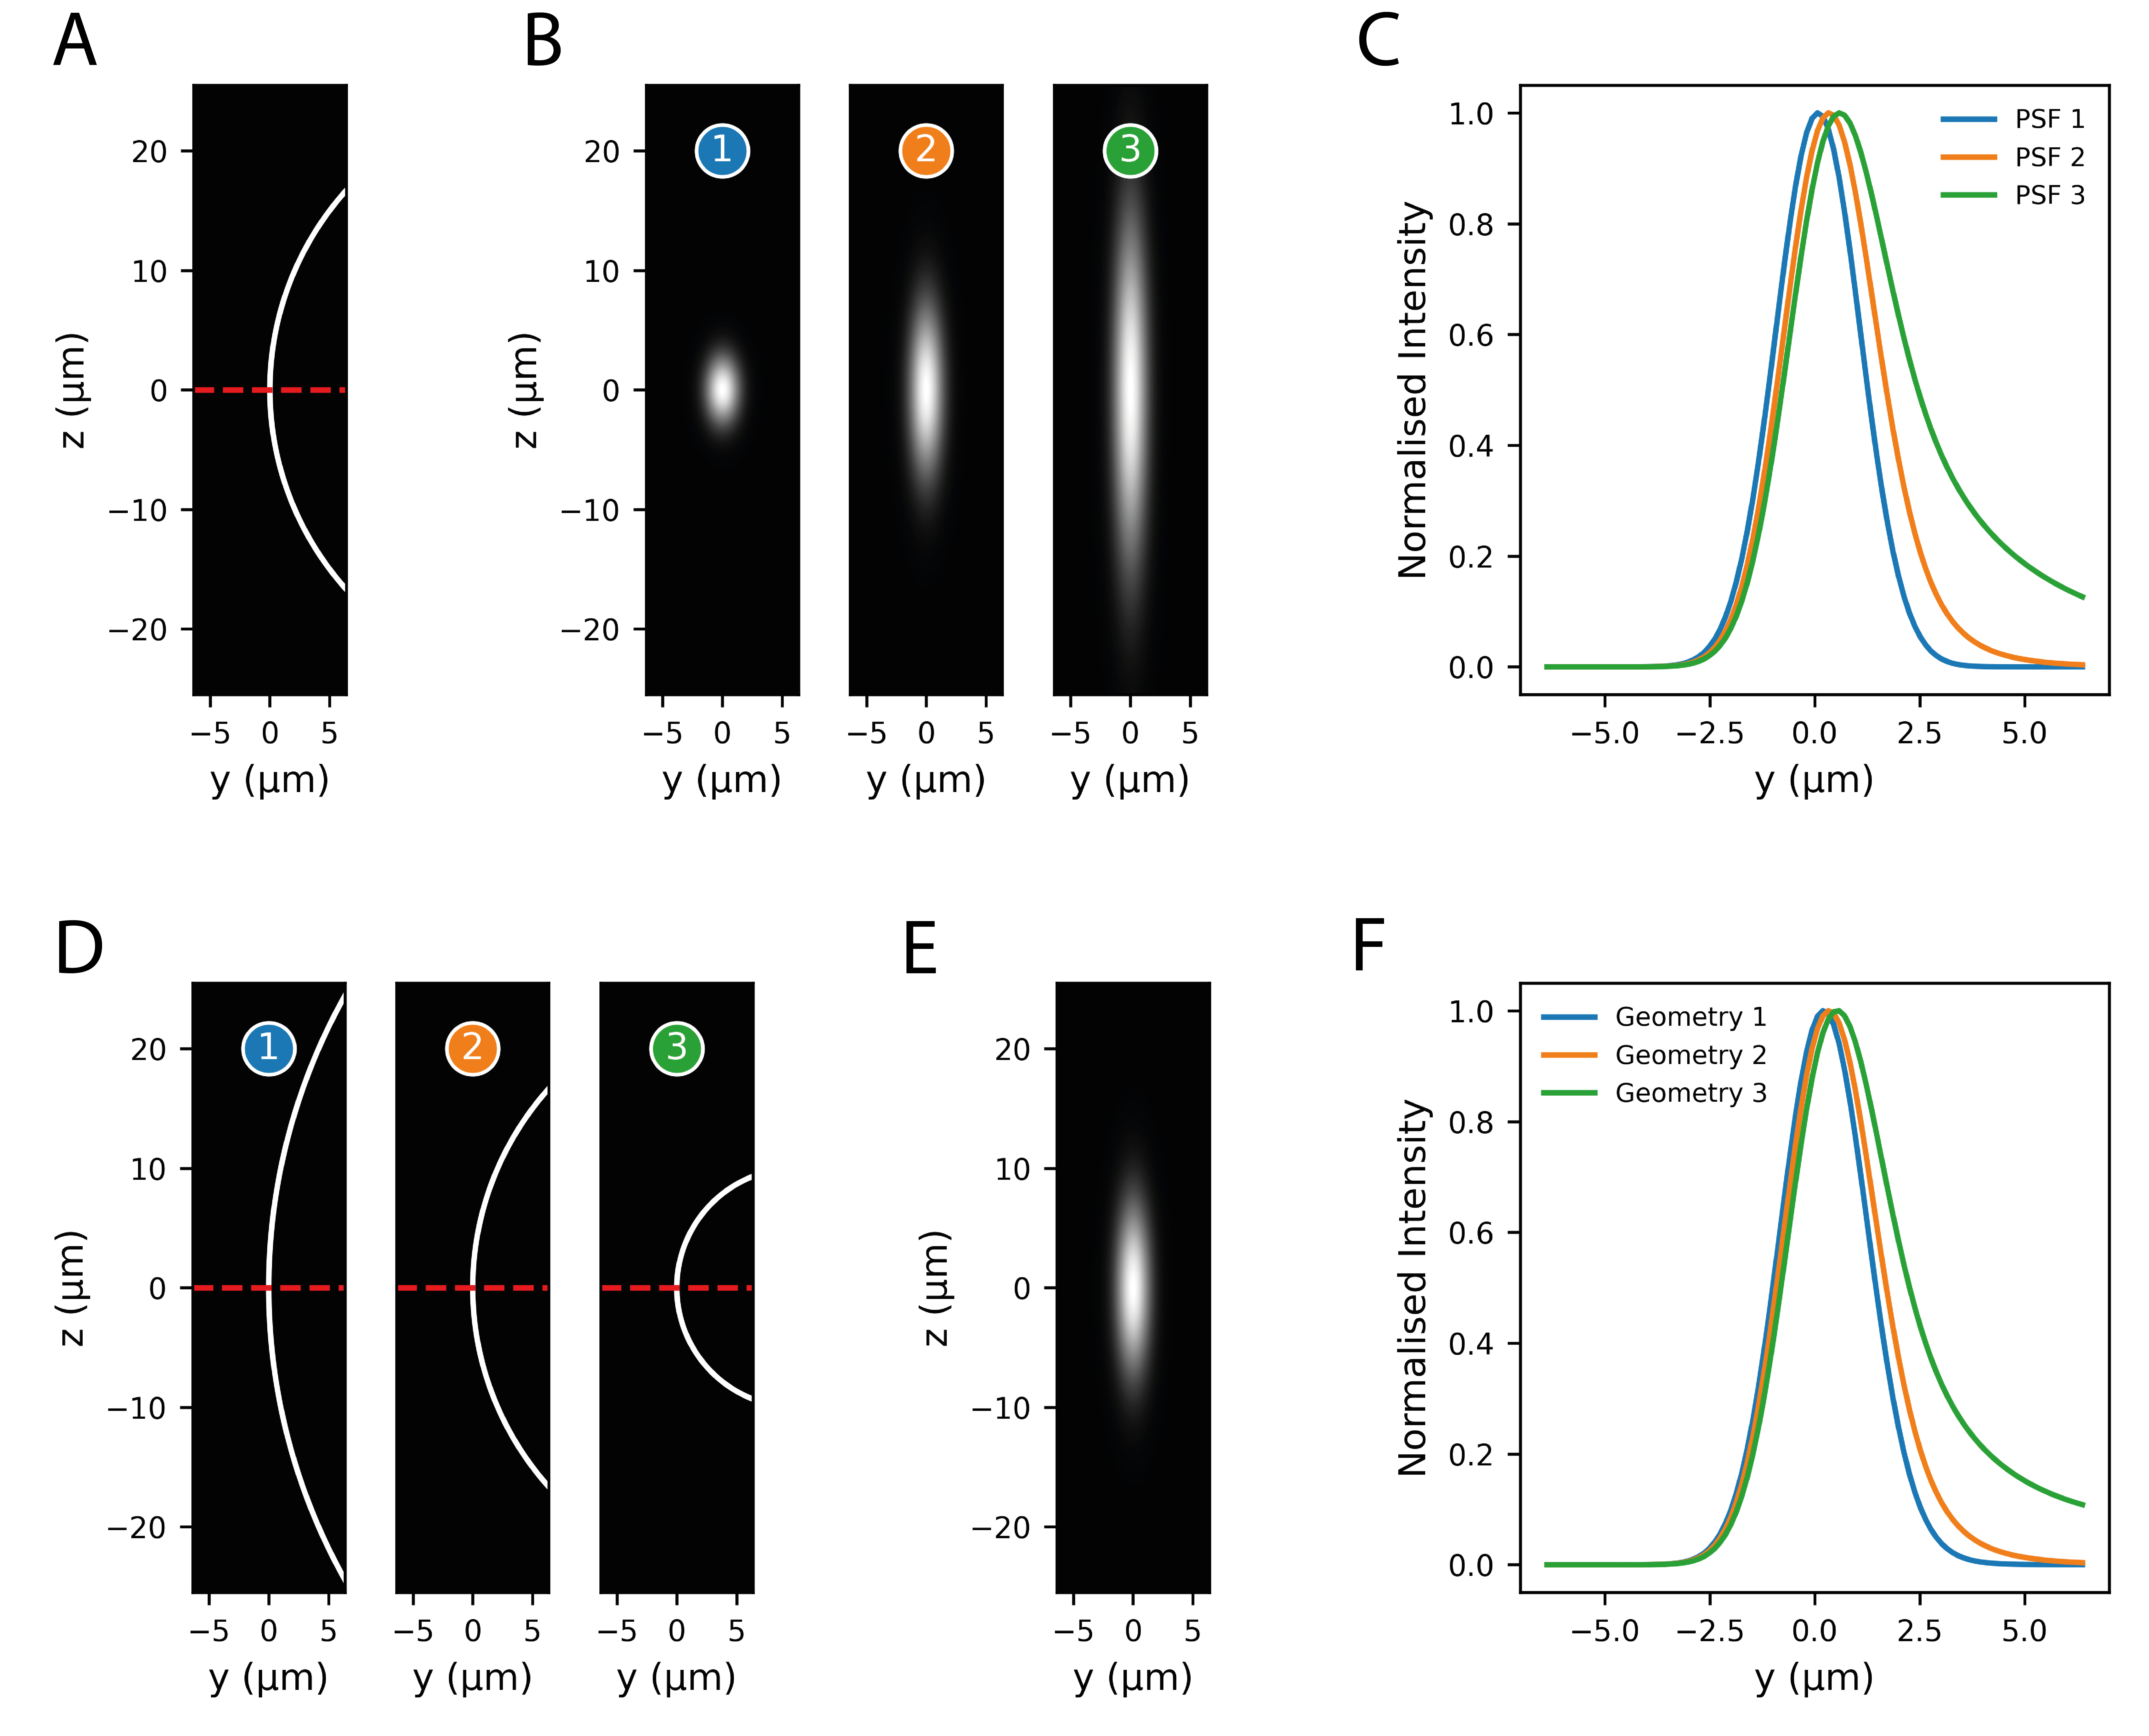
\includegraphics[scale=0.9]{memquant_mem_psf}
\setlength{\abovecaptionskip}{20pt}
\centering
\mycaption{Title}{Caption}
\label{fig:memquant_mem_psf}
\end{figure}

Thus, in order to obtain accurate measures of cytoplasmic and membrane protein concentrations, we need a method to account for out of focus scatter. One common approact to account for out-of-focus scatter is to take a z-stack from across the whole sample, and apply a deconvolution algorithm to the 3D stack to reassign all blurred/scattered light to an in-focus location \citep{Wallace2001}. These methods rely on prior knowledge of the point spread function that applies to the particular sample and imaging set-up, which needs to be as accurate as possible, otherwise artefacts can result. Theoretical methods exist to estimate an appropriate PSF given parameters such as the imaging modality, numerical aperture and emitted light wavelength. Whilst these methods are good at describing blur within the imaging apparatus, scattering within the sample and at the sample-apparatus interface is difficult to model accurately. For this reason, it can be more effective to measure an empirical PSF by imaging the light distribution from a single point source (e.g. a fluorescent bead) under similar sample prep conditions to your sample of interest. However, as PSFs are influenced by scatter within the sample itself, the accuracy of this method depends on how closely the sample environment can be replicated when imaging the beads, which is not trivial. \\

Furthermore, most deconvolution methods assume that the PSF is a constant function throughout the whole image, but in many cases this won't be the case. There may, for example, be refractive index gradients within the sample, which will alter the shape of the PSF depending on location within the sample. Additionally, if there is a mismatch between the refractive index of the immersion and mounting media, as is often unavoidable when imaging live biological samples, then the PSF will usually vary with depth as spherical aberrations will be introduced deeper into the sample. A PSF from a fluorescent bead located directly below the coverslip will not capture either of these phenomena.\\

In reality, given all of these confounding factors, an accurate description of the PSF that applies to a given sample of interest is often an unachievable goal. Whilst deconvolution with a suboptimal PSF may be sufficient for many qualitative applications, accurate quantitative measurements cannot be guaranteed. For this reason, I opted against using a PSF-based deconvolution approach to account for out-of-plane scattering.\\

% transition

Fortunately, in this particular case, matters are greatly simplified by the fact that the geometry of protein distribution are usually highly consistent. Not only is the shape of embryos highly consistent, but PAR protein distributions within the embryo also tend to display rotational symmetry (at least during normal polarity development in P0), meaning that protein distributions in planes above and below the focal plane tend to be similar/identical to those seen at the focal plane (much like the simulations in figs x and x). Optical properties are also not expected to change from sample to sample, or from location to location around the circumference of an embryo.\\

Together, these features imply that, for cytoplasmic or membrane protein, the normalised shape of the cross-cortex profile measured at the midplane should be some consistent function, that shouldn’t vary much between embryos or spatially around the circumference of an embryo. A change in local or global concentration should amount to a rescaling of this profile, but shouldn't change the normalised shape. Where there is a mix of cytoplasmic and cortical protein, the total measured cross-cortex profile will then be a sum of these two contributions. Therefore, if one has prior knowledge of the expected shape of the cross-cortex profile for cytoplasmic-only and membrane-only protein, then measured profiles can be fit as the sum of these two contributions, and membrane/cytoplasmic concentrations extracted as the amplitudes of the two signal components.\\

Thus, a key step in the path to accurate quantification is the ability to measure these reference profiles. As mentioned previously, cytoplasmic reference profiles can easily be obtained by analysing cells in which all protein is cytoplasmic. Indeed, Reich used an approach half-way between the Gross method and the method that I am proposing, replacing the error-function description of cytoplasmic signal with his arbitrary, measured, cytoplasmic reference profile. Thus, total signals were fit as the sum of a Gaussian profile and this arbitrary cytoplasmic reference profile, which resulted in a far better ability of the model to fit the shape of measured profiles.\\

Whilst this move is a significant step in the right direction, the problem remains of how best to account for out of focus cortical light. This presents a challenge: whilst it is relatively easy to directly measure a cytoplasmic reference profile (you just need a reference image in which all signal is cytoplasmic), the same is not true for a membrane profile as it is difficult/impossible to find a reference case in which all protein is membrane bound. To extend the Reich method to account for out-of-focus membrane protein, I attempted to find alternative methods to get an approximation of the membrane reference profile. An initial idea, which involved staining the exterior of the eggshell with a fluorescent dye, proved technically challenging and not reproducible.\\

Instead, the problem becomes simplified when one considers that, even in cases where the cortex is polarised, the cytoplasm of most PAR proteins should be uniform (although exceptions do exist in the case of PAR-1 and PAR-3, where true cytoplasmic gradients have been observed, although the basis for this is poorly understood). Thus, straightened cortices can be modelled as a uniform cytoplasmic component, defined by a cytoplasmic reference profile (Rc) and a single, uniform, cytoplasmic concentration (C), plus a polarised membrane component, defined by a membrane reference profile (Rm) and a nonuniform membrane concentration profile (M). This is shown in fig x. This is essentially a generalisation of the methods used by Gross and Reich, but proposes the use of arbitrary membrane and cytoplasmic reference profiles rather than mathematical functions (e.g. Gaussian, error function).\\

Rc can easily be predefined (fig x). If we assume for a second that Rm is also predefined, then M and C for a given embryo can be determined by fitting a straightened image to this model. (At this point these values will be in arbitrary units, but I’ll come back to this point). Whilst Rm is in fact not predefined, given the constraints imposed by cytoplasmic uniformity, it arises that only a model with an appropriate Rm will be able to create simulated images that closely match experimental images. (Imagine, for example a model with a Gaussian membrane reference profile, which would clearly fail to capture the graded internal signal). Therefore, under conditions such as these, in which we have a uniform cytoplasmic component and a graded membrane component, Rm need not be predefined, and can simply be fit to the data along with the concentration parameters. To perform this kind of optimisation, I have used a gradient descent approach based on differentiable programming, which is described below.\\

\begin{figure}[!h]
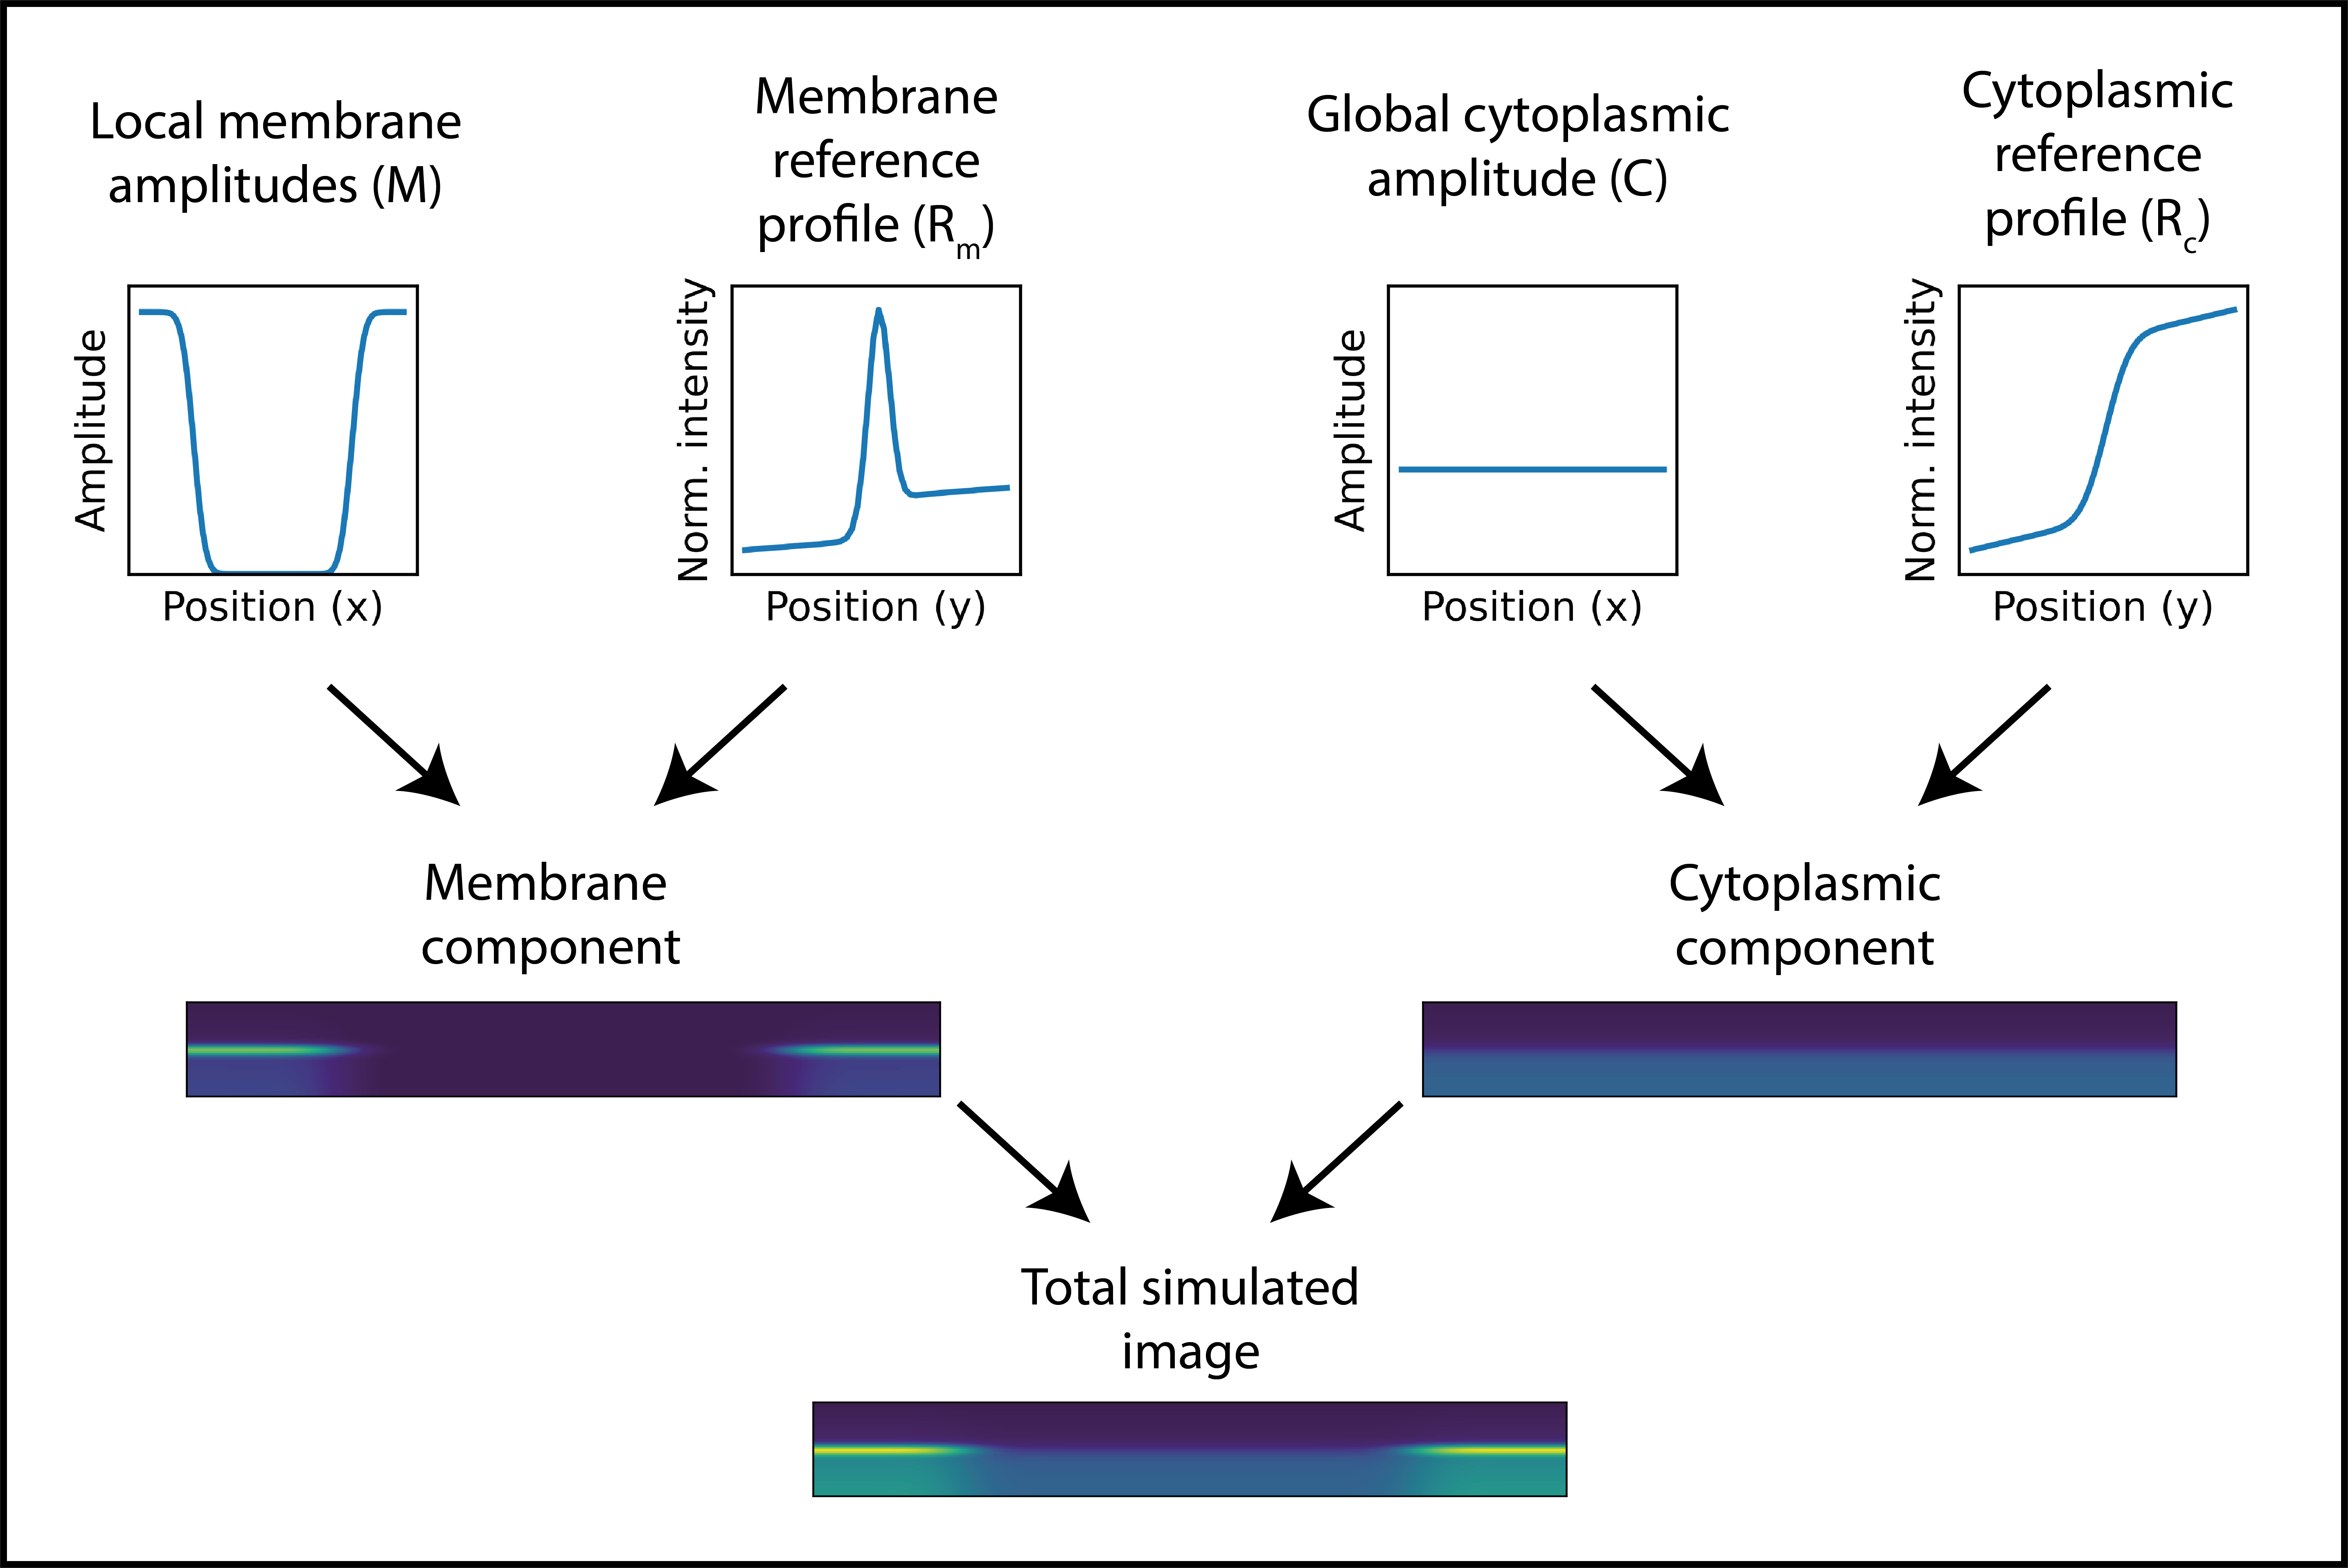
\includegraphics[scale=1.1]{memquant_model_schematic}
\setlength{\abovecaptionskip}{20pt}
\centering
\mycaption{Title}{Caption}
\label{fig:memquant_model_schematic}
\end{figure}

\subsubsection{A gradient descent protocol for image quantification}

Gradient descent is a popular optimisation strategy used for a number of machine learning applications. The idea is to calculate the partial derivative of each input parameter with respect to a loss term (mean squared error). A negative gradient for a parameter would imply that an increase in that parameter would decrease overall loss, whereas a positive gradient would imply the opposite. Therefore, to reduce loss, each input parameter can be adjusted according to its partial derivative. Starting with a set of initial conditions, this procedure is then iteratively repeated, adjusting parameters and calculating new gradients at each step, until the loss term reaches a minimum. \\

The utility of these methods has been greatly advanced in recent years by the advent of differentiable programming tools. Commonly used for deep learning, although generalisable to other problems, these tools greatly speed up computation for complex optimisation procedures by automatically calculating gradients at every step, rather than relying on numerical methods, using a process called backpropagation. In addition, extensions to the basic gradient descent algorithm (e.g. Adam) have proven effective at speeding up convergence and preventing entrapment in local minima. \\

In the case of this particular problem, this procedure is described in figure x. Given a set of parameters (M, C, Rm, Rc), a forward propagation step simulates an image (fig x), and then this is compared to a ground truth image to calculate an error term. Backpropagation then calculates the gradient of each of the input parameters with respect to this error term. At this point, we can adjust some or all of the input parameters according to these gradients. Repeating this cycle of forward and back propagation will then lead to a gradual optimisation in these parameters, until a minimum is reached. \\

\begin{figure}[!h]
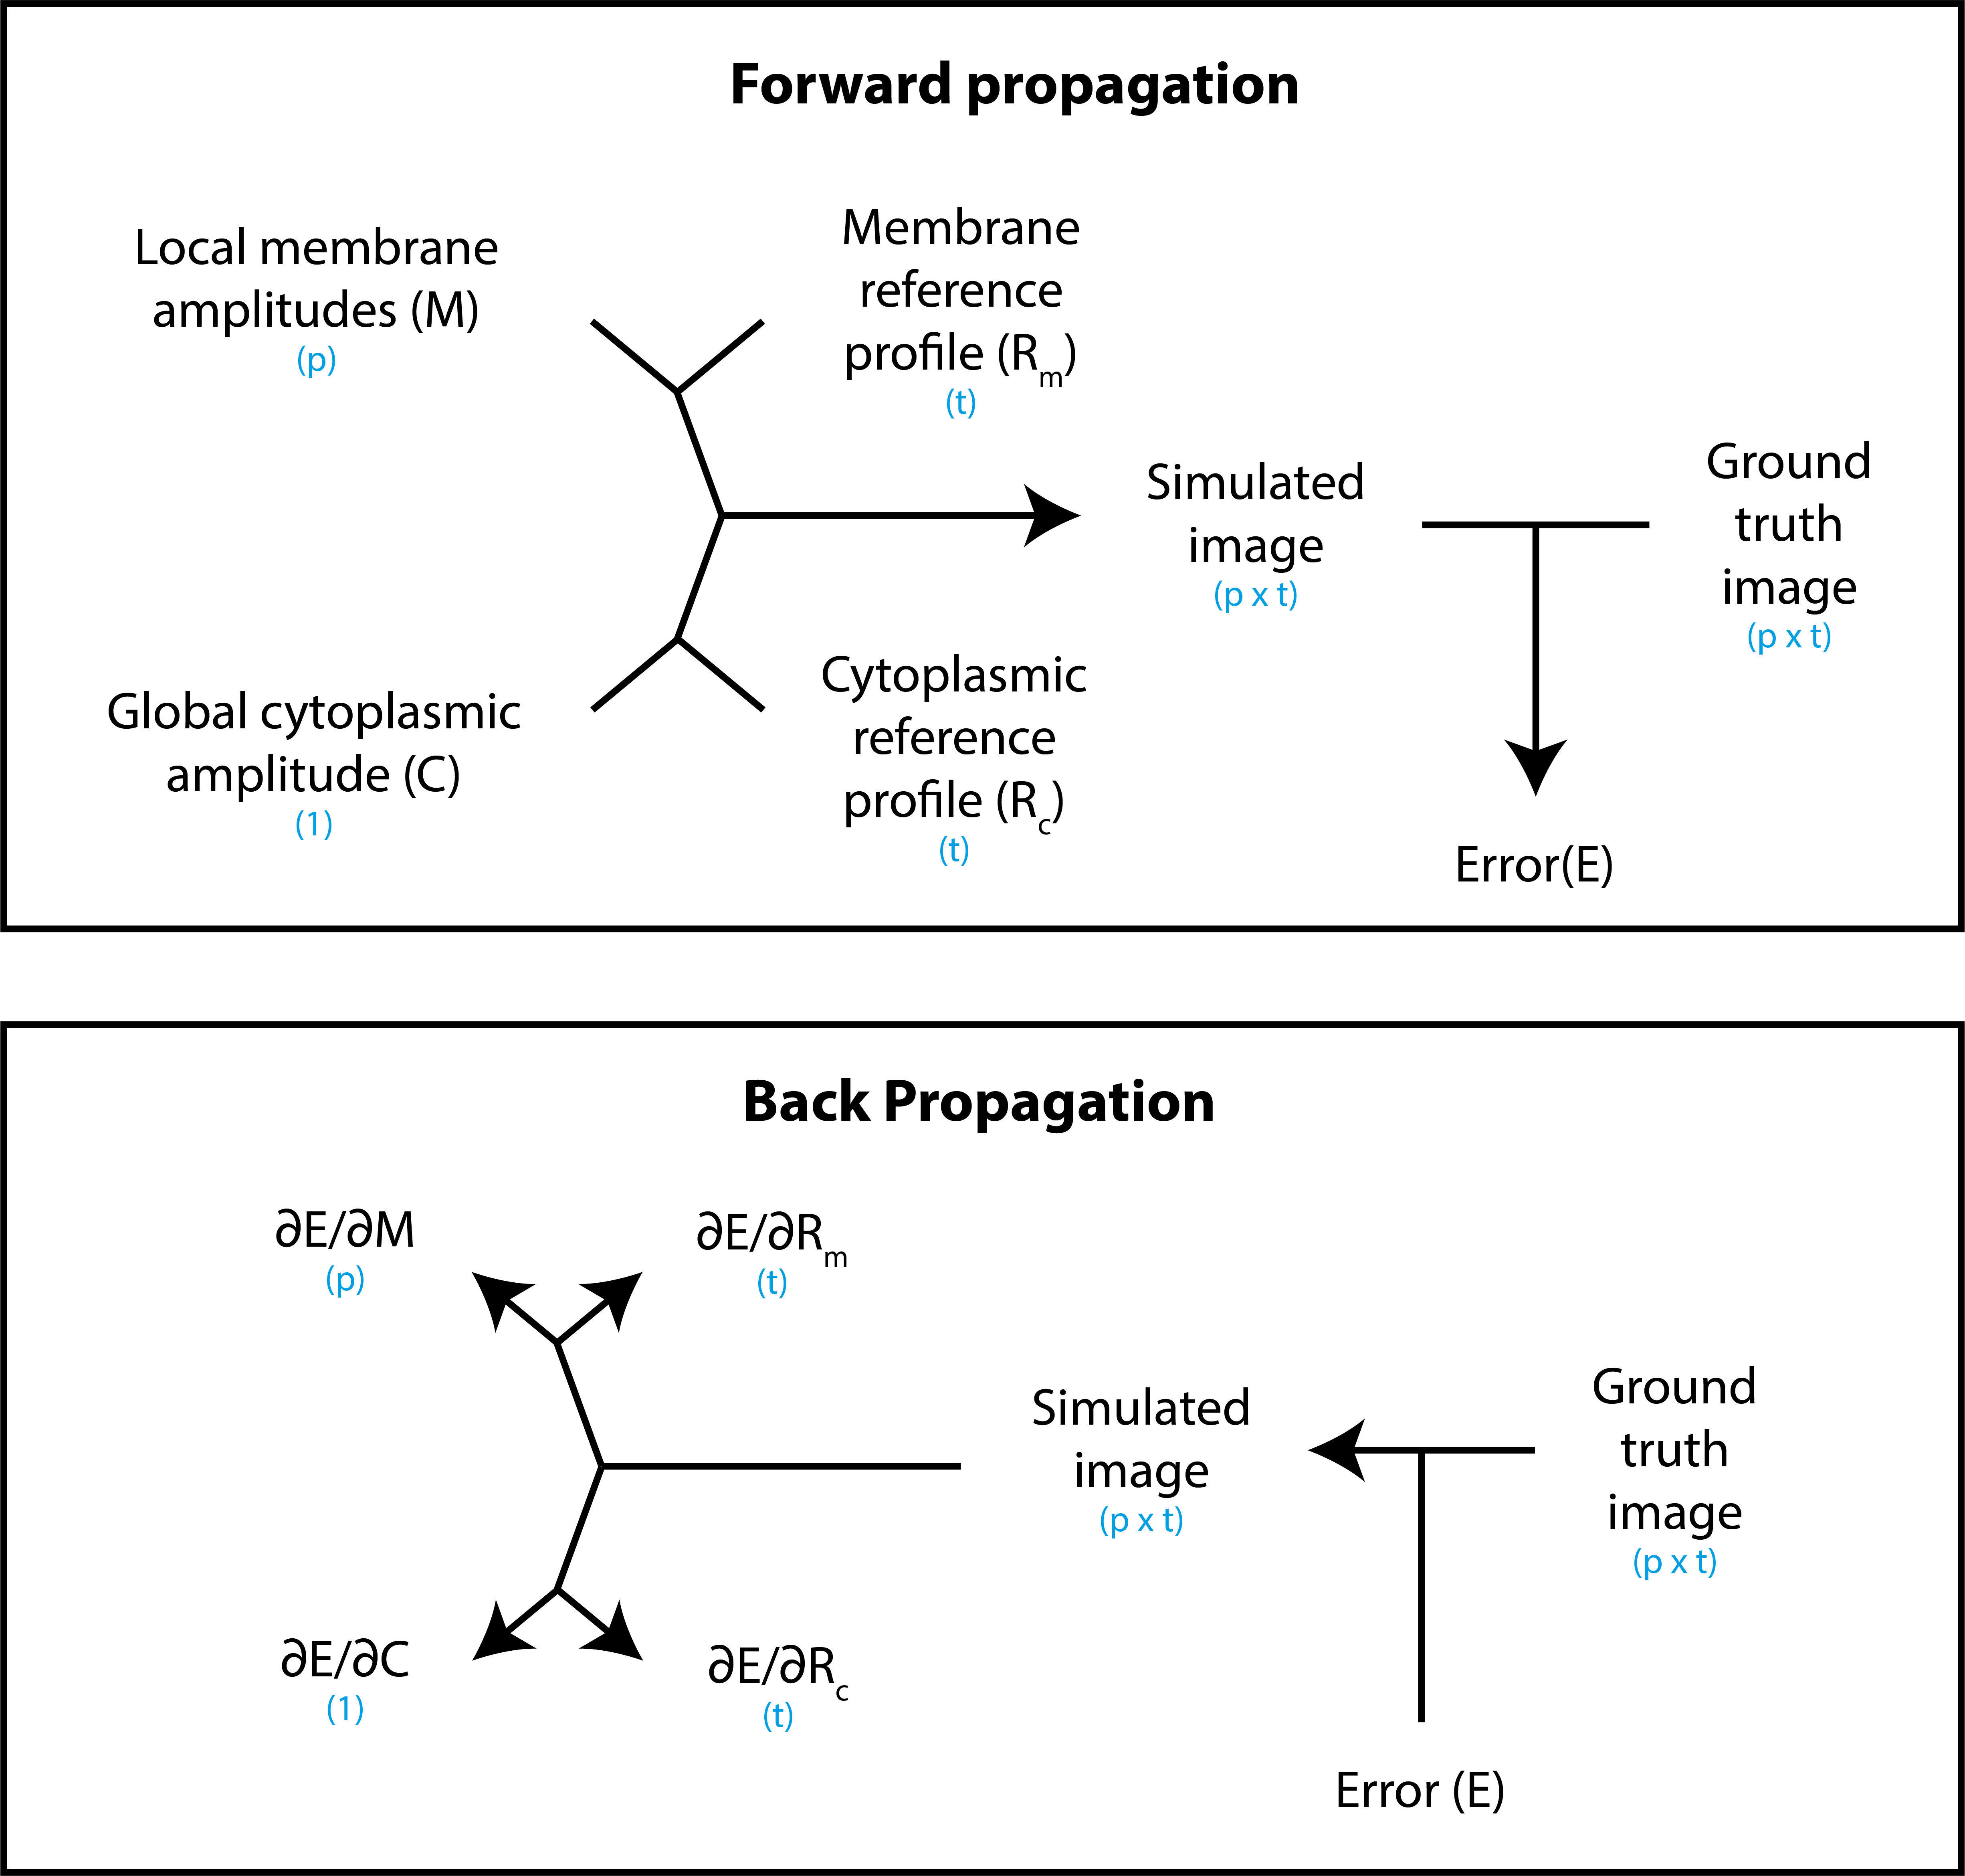
\includegraphics[scale=1.1]{memquant_forward_and_back_propagation}
\setlength{\abovecaptionskip}{20pt}
\centering
\mycaption{Title}{Caption}
\label{fig:memquant_forward_and_back_propagation}
\end{figure}

To test this approach, I first applied it to images of polarised PAR-2. Built using the differentiable programming package Tensorflow (cite: Abadi), the model was initiated with all concentrations (M and C) equal to zero, and Rm initiated as a Gaussian. For Rc I used a measured profile (fig x), and this was not adjusted during training (fig xa). Using an Adam optimiser with a learning rate of 0.01, all other parameters (M, C and Rm) were then adjusted iteratively until a plateau was reached (250 steps), as shown in fig xb. As shown in fig xc, the final simulated image, composed of a uniform cytoplasmic component and a nonuniform membrane component, fits closely to the ground truth image.\\


\begin{figure}[!h]
\includegraphics[scale=1]{memquant_membg_training}
\setlength{\abovecaptionskip}{20pt}
\centering
\mycaption{Title}{Caption}
\label{fig:memquant_membg_training}
\end{figure}

% more here on reproducibility.

\subsubsection{Segmentation}

In addition to the parameters already mentioned, the model also includes a series of alignment parameters, which are also trained by gradient descent, allowing the model to freely align to the data in the x direction. As a result, ground truth images do not need to be accurately segmented prior to optimisation, and rough manual ROIs are fine to use. This is particularly useful for movies, where, even if the embryo undergoes small shape changes, only a single manual ROI needs to be provided. Another nice outcome of this is that these offset parameters can then be used to refine the original ROI, meaning that the method can serve as a tool for computational segmentation. Refined ROIs can then be used to restraighten the cortex, and optimisation repeated.\\

% figure explaining this

\clearpage
\subsubsection{Benchmarking the method}

The method described so far is limited to a special case of images with polarised membrane concentrations. However, as discussed previously, the optimised membrane reference profile, which is a function of local geometry and optical properties, should be applicable to all embryos. Therefore, much like we used a predefined cytoplasmic reference profile when fitting polarised PAR-2, images of proteins without a polarised membrane can be quantified by using an Rm derived from a calibration procedure on polarised images. \\

To test this method, I performed quantification on images of PH with variable expression levels, obtained by performing an RNAi rundown using XFP (see Methods). In this case, I used a predefined Rm and Rc, and only optimised M and C (as well as the alignment parameters described in the previous section), fig xa. Compatible with expected linear membrane binding kinetics, we can see that the method gives a tight linear relationship between cytoplasmic and membrane concentrations. N2s are also accurately describes as having cytoplasmic and membrane concentrations of zero.\\

\begin{figure}[!h]
\includegraphics[scale=1]{memquant_benchmarking_ph_rundown}
\setlength{\abovecaptionskip}{20pt}
\centering
\mycaption{Title}{Caption}
\label{fig:memquant_benchmarking_ph_rundown}
\end{figure}

I next investigated how robust the method is to changing signal-to-noise ratios, using three PH embryos with varying levels of expression. Adding pixel noise to these images may be expected to add noise to the resulting concentrations, but shouldn’t bias the data in any direction. As seen in figues xc and xd, this is precisely the case for all three PH embryos. Quantification of N2s is also not biased by noise (fig xc,d grey points). In addition, segmentation results are strikingly robust to noise, even at high noise levels that render embryos near-invisible to the human eye (fig xb).\\

\begin{figure}[!h]
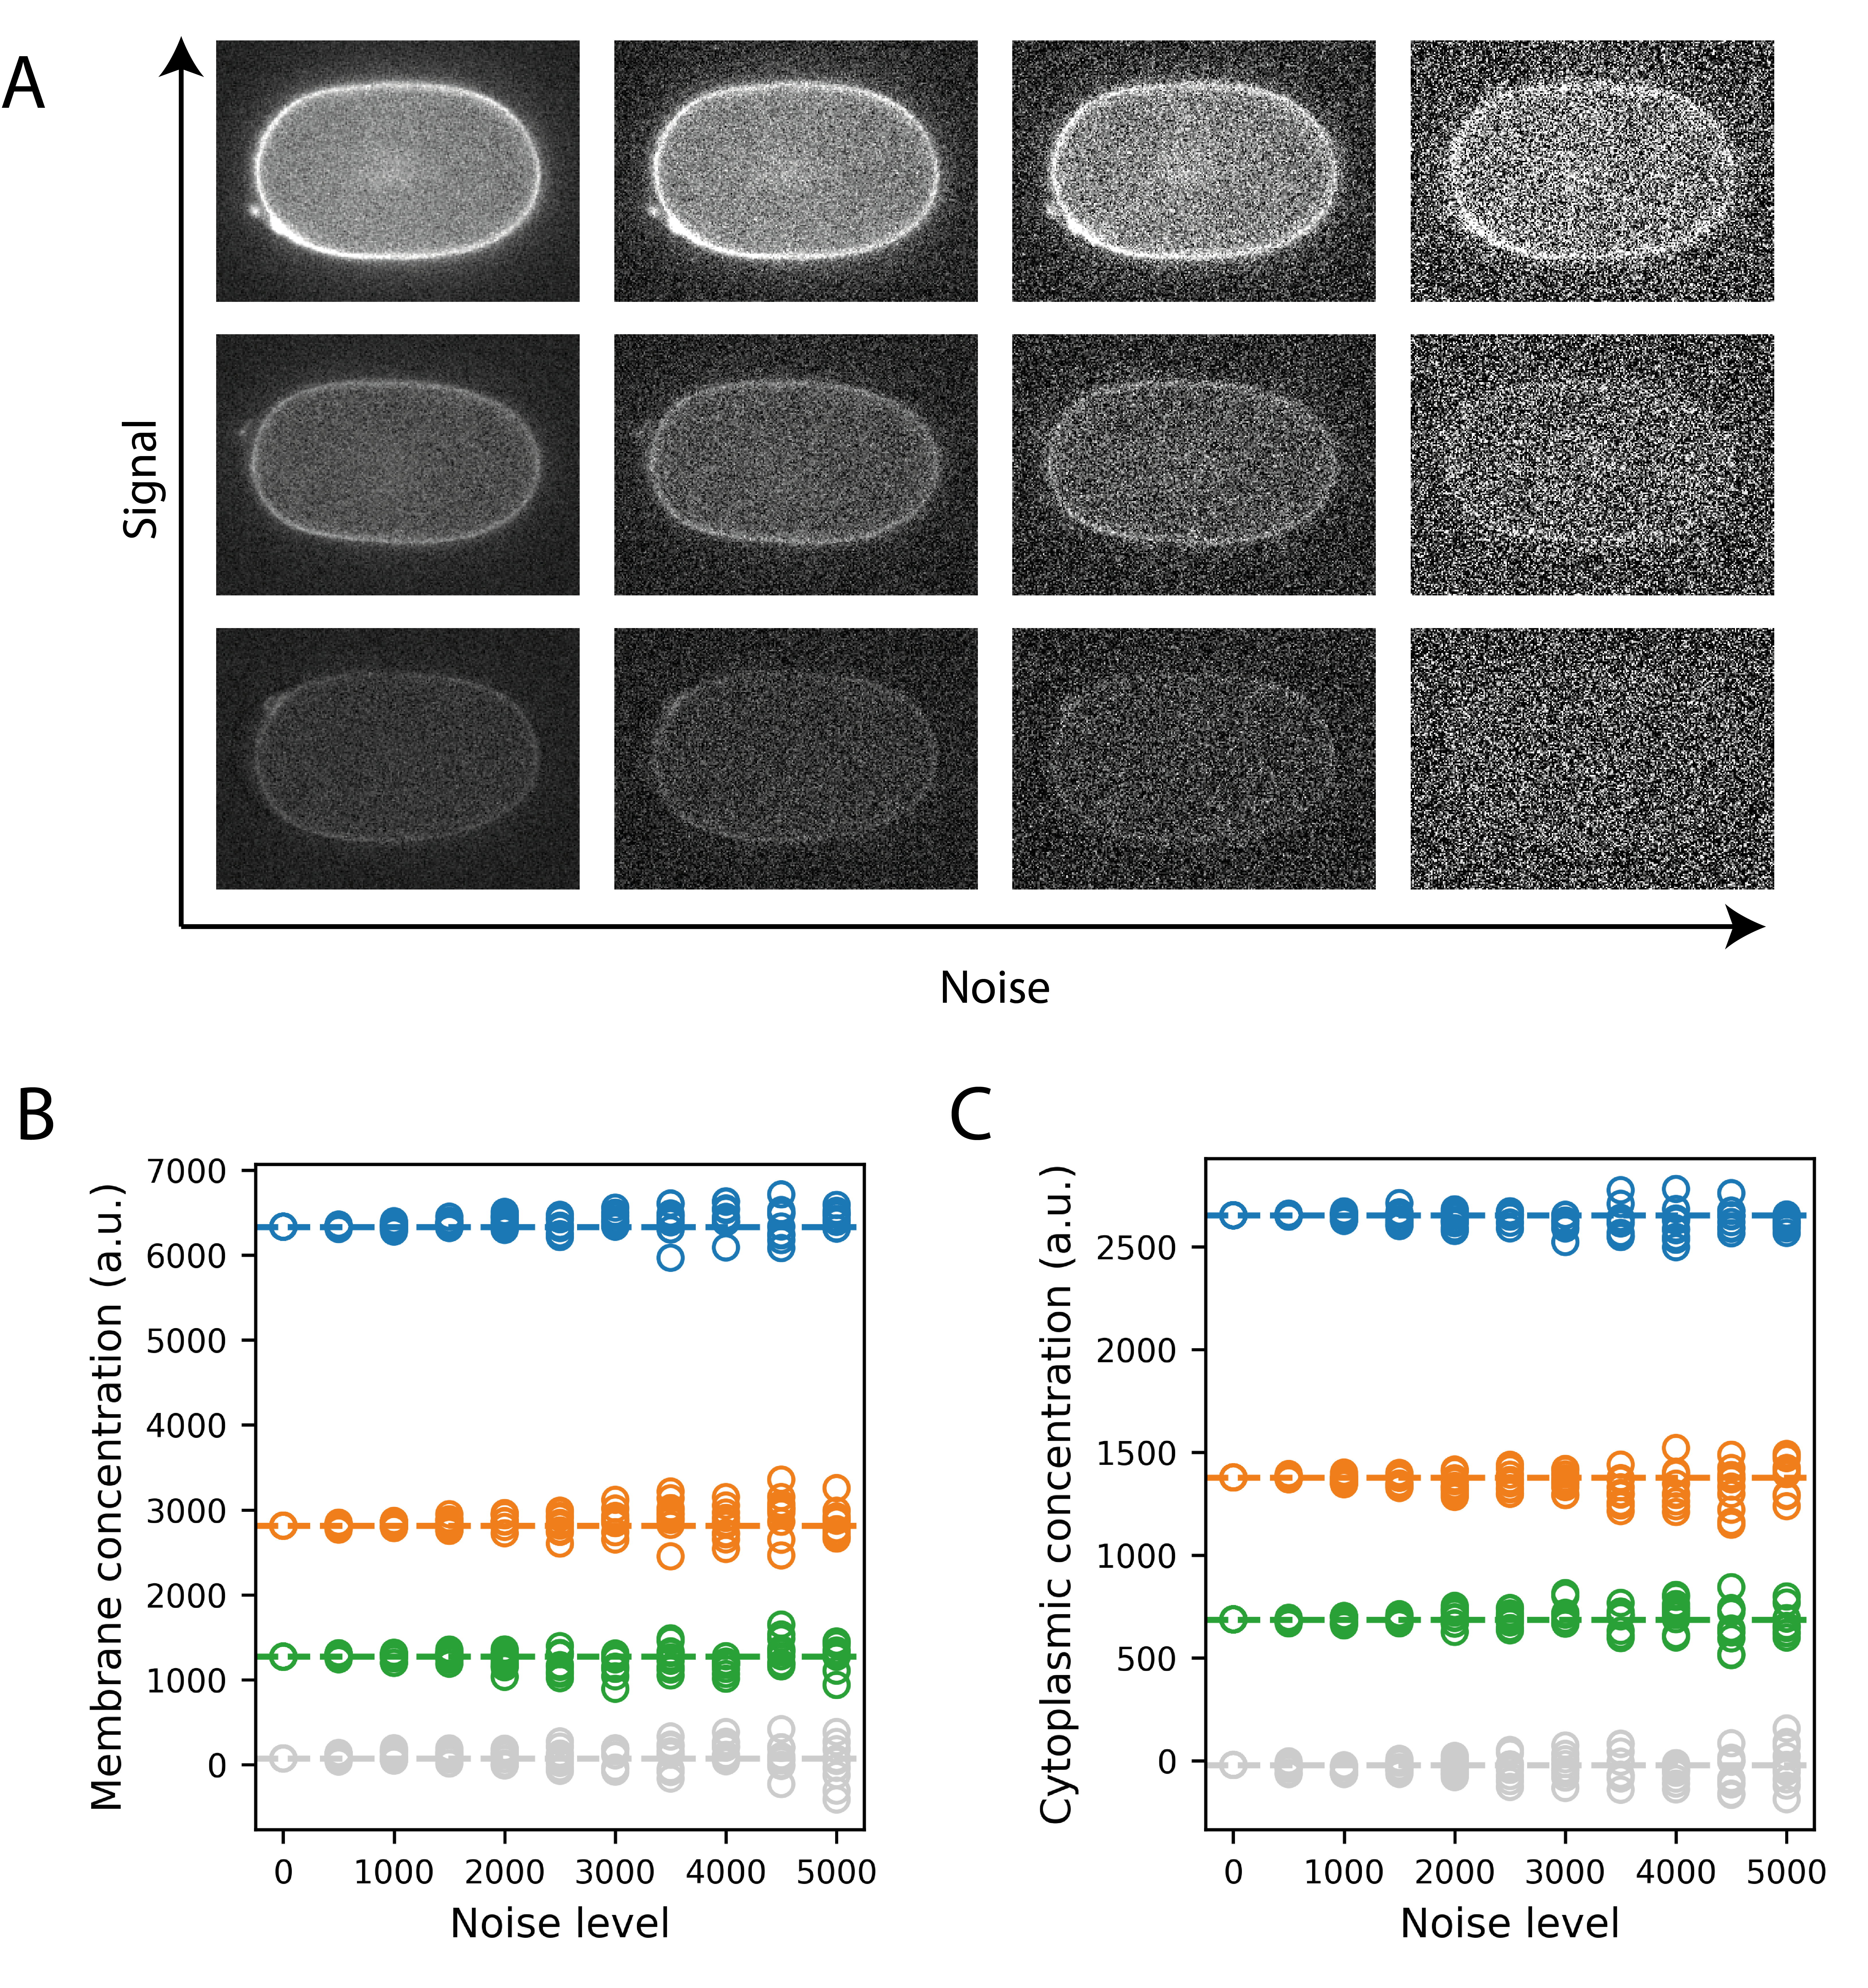
\includegraphics[scale=0.85]{memquant_benchmarking_noise}
\setlength{\abovecaptionskip}{20pt}
\centering
\mycaption{Title}{Caption}
\label{fig:memquant_benchmarking_noise}
\end{figure}


\subsubsection{Calibrating concentration units}

As M and C are in arbitrary units (effectively in units of their own respective reference profile), a conversion parameter, is required to put them in comparable units. To calibrate this conversion parameter, I quantified the effects on M and C measurements of redistributing a fixed pool of protein from the cytoplasm to the membrane. To do this, I used an optogenetics system with a membrane bound PH::eGFP::LOV to move a cytoplasmic pool of ePDZ::mCherry to the membrane (Fielmich et al., 2018). Embryos were exposed to blue light for 10 seconds, which promotes binding between ePDZ and LOV, leading to a rapid uniform recruitment of ePDZ::mCherry to the membrane and a reduction in the concentration in the cytoplasm (fig x). Where ePDZ mcherry is expressed alone, this localisation shift isn’t observed (fig x, grey).\\

\begin{figure}[!h]
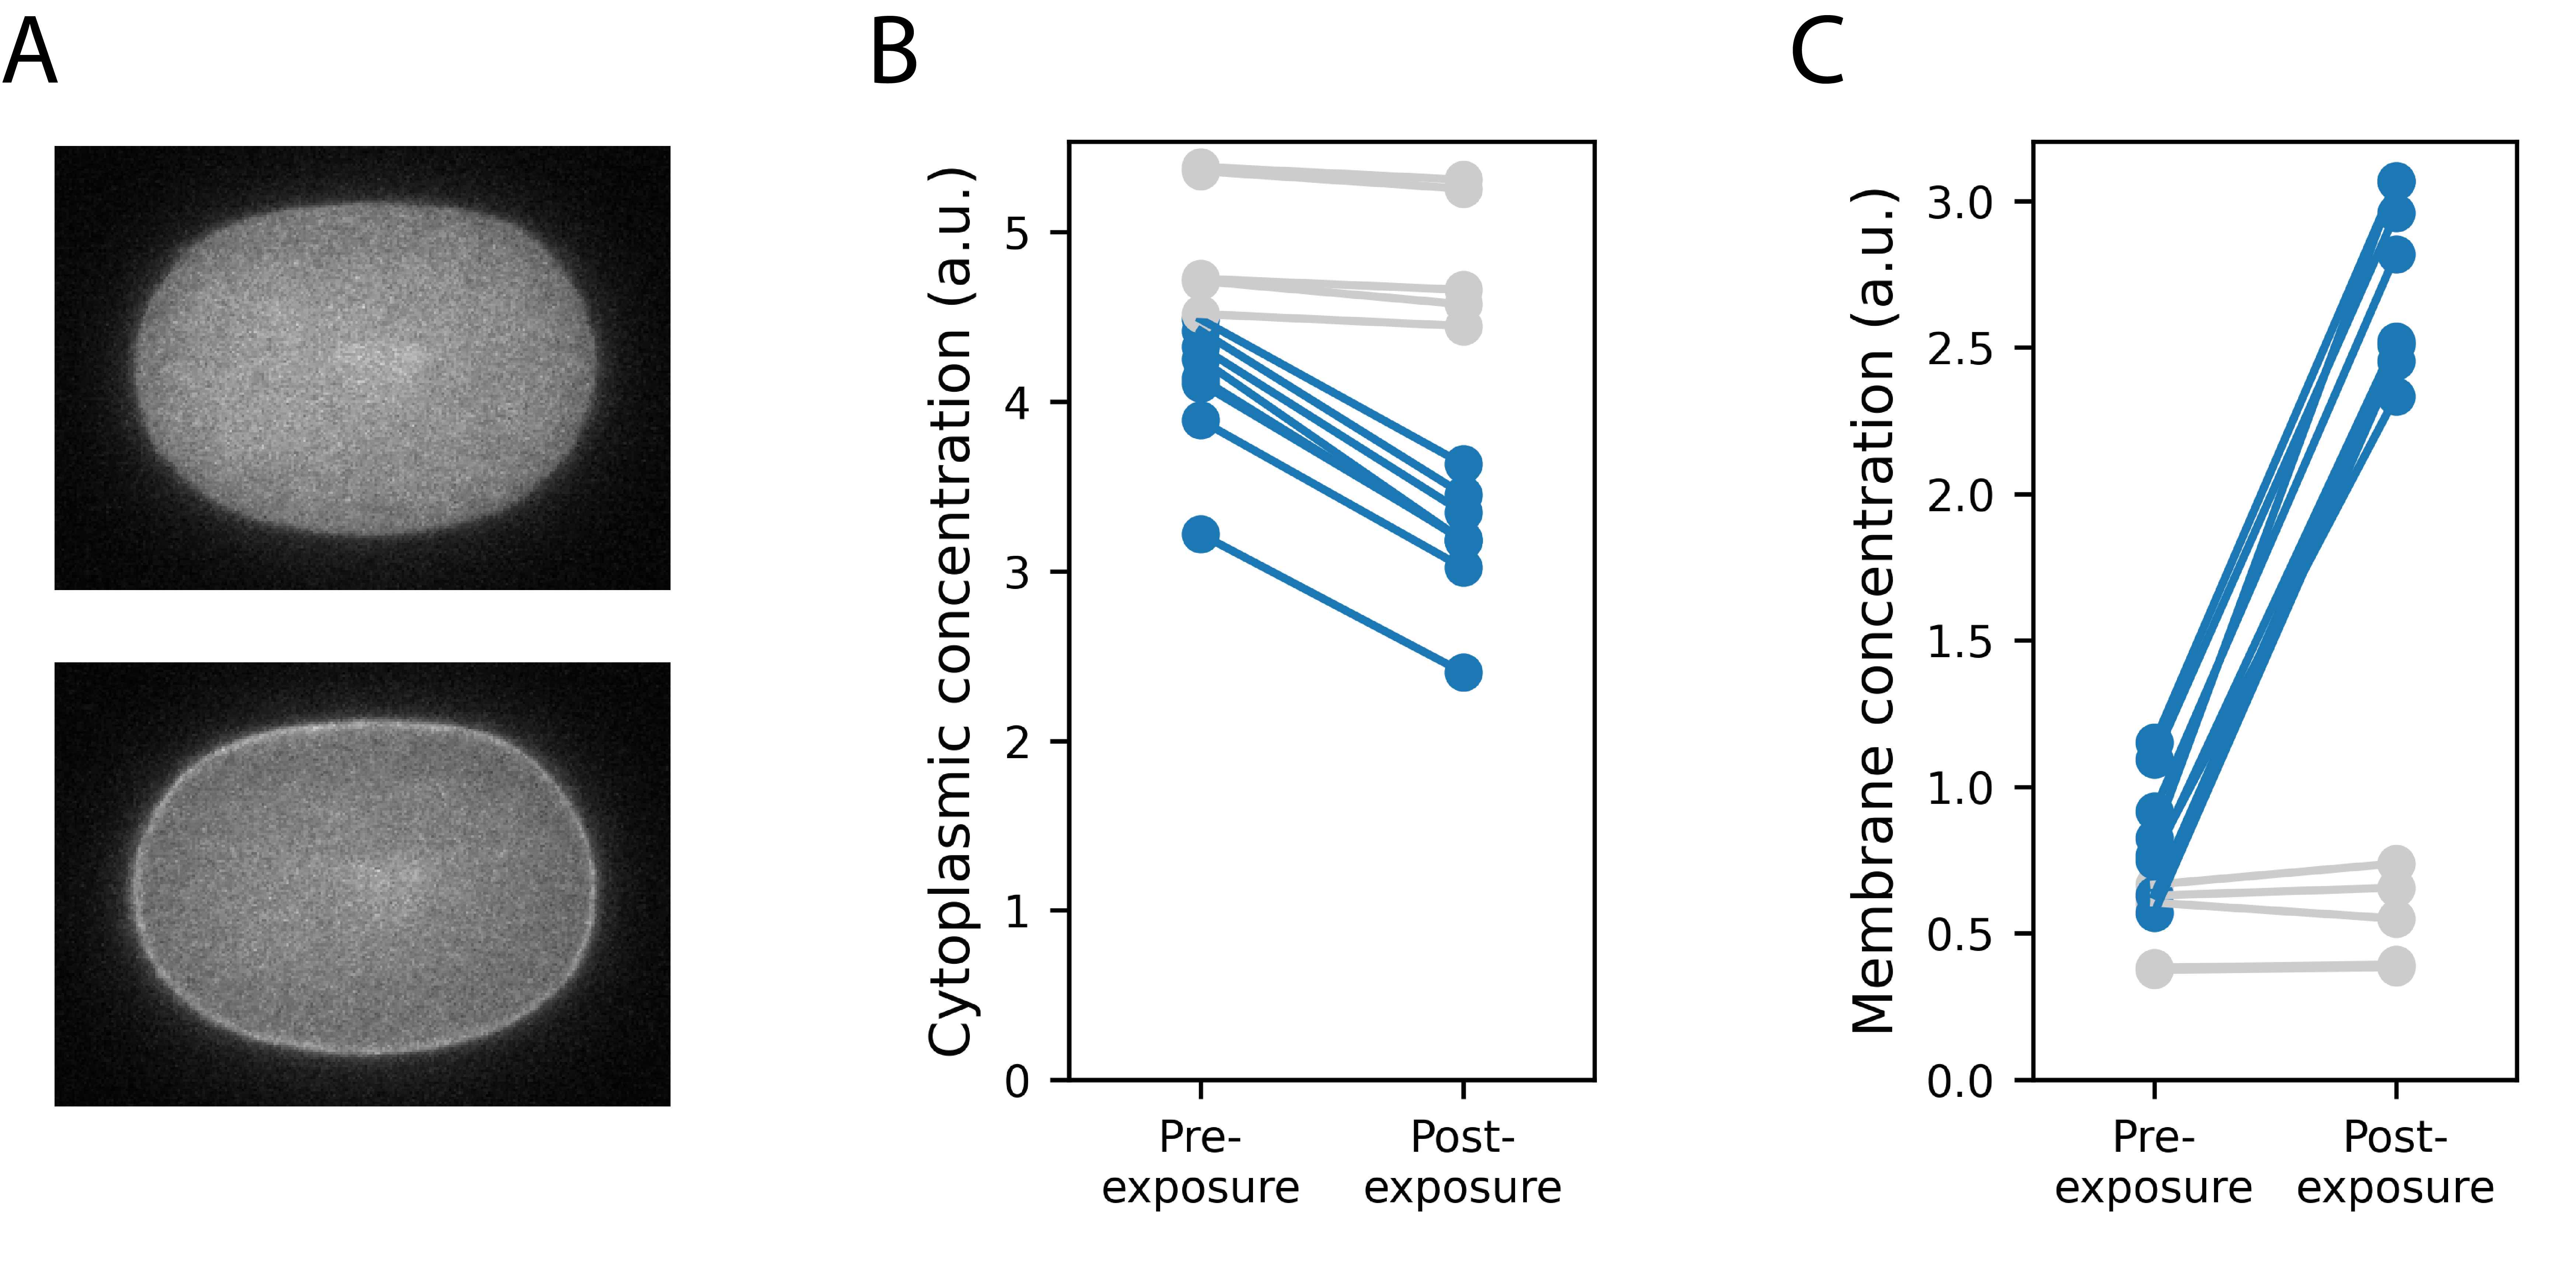
\includegraphics[scale=1]{memquant_optogenetics}
\setlength{\abovecaptionskip}{20pt}
\centering
\mycaption{Title}{Caption}
\label{fig:memquant_optogenetics}
\end{figure}


Whilst there is significant relocalisation, the total amount of protein can be assumed to be constant. This total amount, T, can be expressed as the C value that would be expected if all tagged molecules were in the cytoplasm, given by equation x where $\psi$ is the surface-area to volume ratio of the cell. Given that M is in different arbitrary units to C, a conversion parameter, c, is required:

\begin{equation}
\tau = C + \psi c M
\label{eq:T}
\end{equation}

Given that T must be the same before and after exposure, c can be calculated, on an embryo by embryo basis, by comparing the gain in M to the loss in C:\\

\begin{equation}
c = \frac{C_{pre \textrm{-} exposure} - C_{post  \textrm{-} exposure}}{\psi (M_{post  \textrm{-} exposure} - M_{pre  \textrm{-} exposure})}
\label{eq:c}
\end{equation}

Performing this analysis gives a value of c = x+- x, which can be used to put M and C in common units. Note that these concentrations are still arbitrary in the sense that they give no indication of absolute concentrations (i.e. absolute number of molecules per unit area). For much of the analysis in the following sections, where the aim is to measure membrane affinities (membrane to cytoplasmic ratios) this will not be an issue, although I’ll return to this point in section x.\\


\clearpage
\subsubsection{Discussion}

%%%%%%%%%%%%%%%%%%%%%%%%%%%%%%%%%%%%%%%%%%%%%%%%%%%%%%%%%%
\clearpage
\section{Identifying core patterning behaviours of PAR-2}

% Note: previous studies have shown that PAR-2 can maintain domains once formed, but hasn't been demonstrated whether PAR-2 can break symmetry without clearance of aPARs.

\subsection{PAR-2 polarity in systems with uniform aPAR}

\begin{figure}[!h]
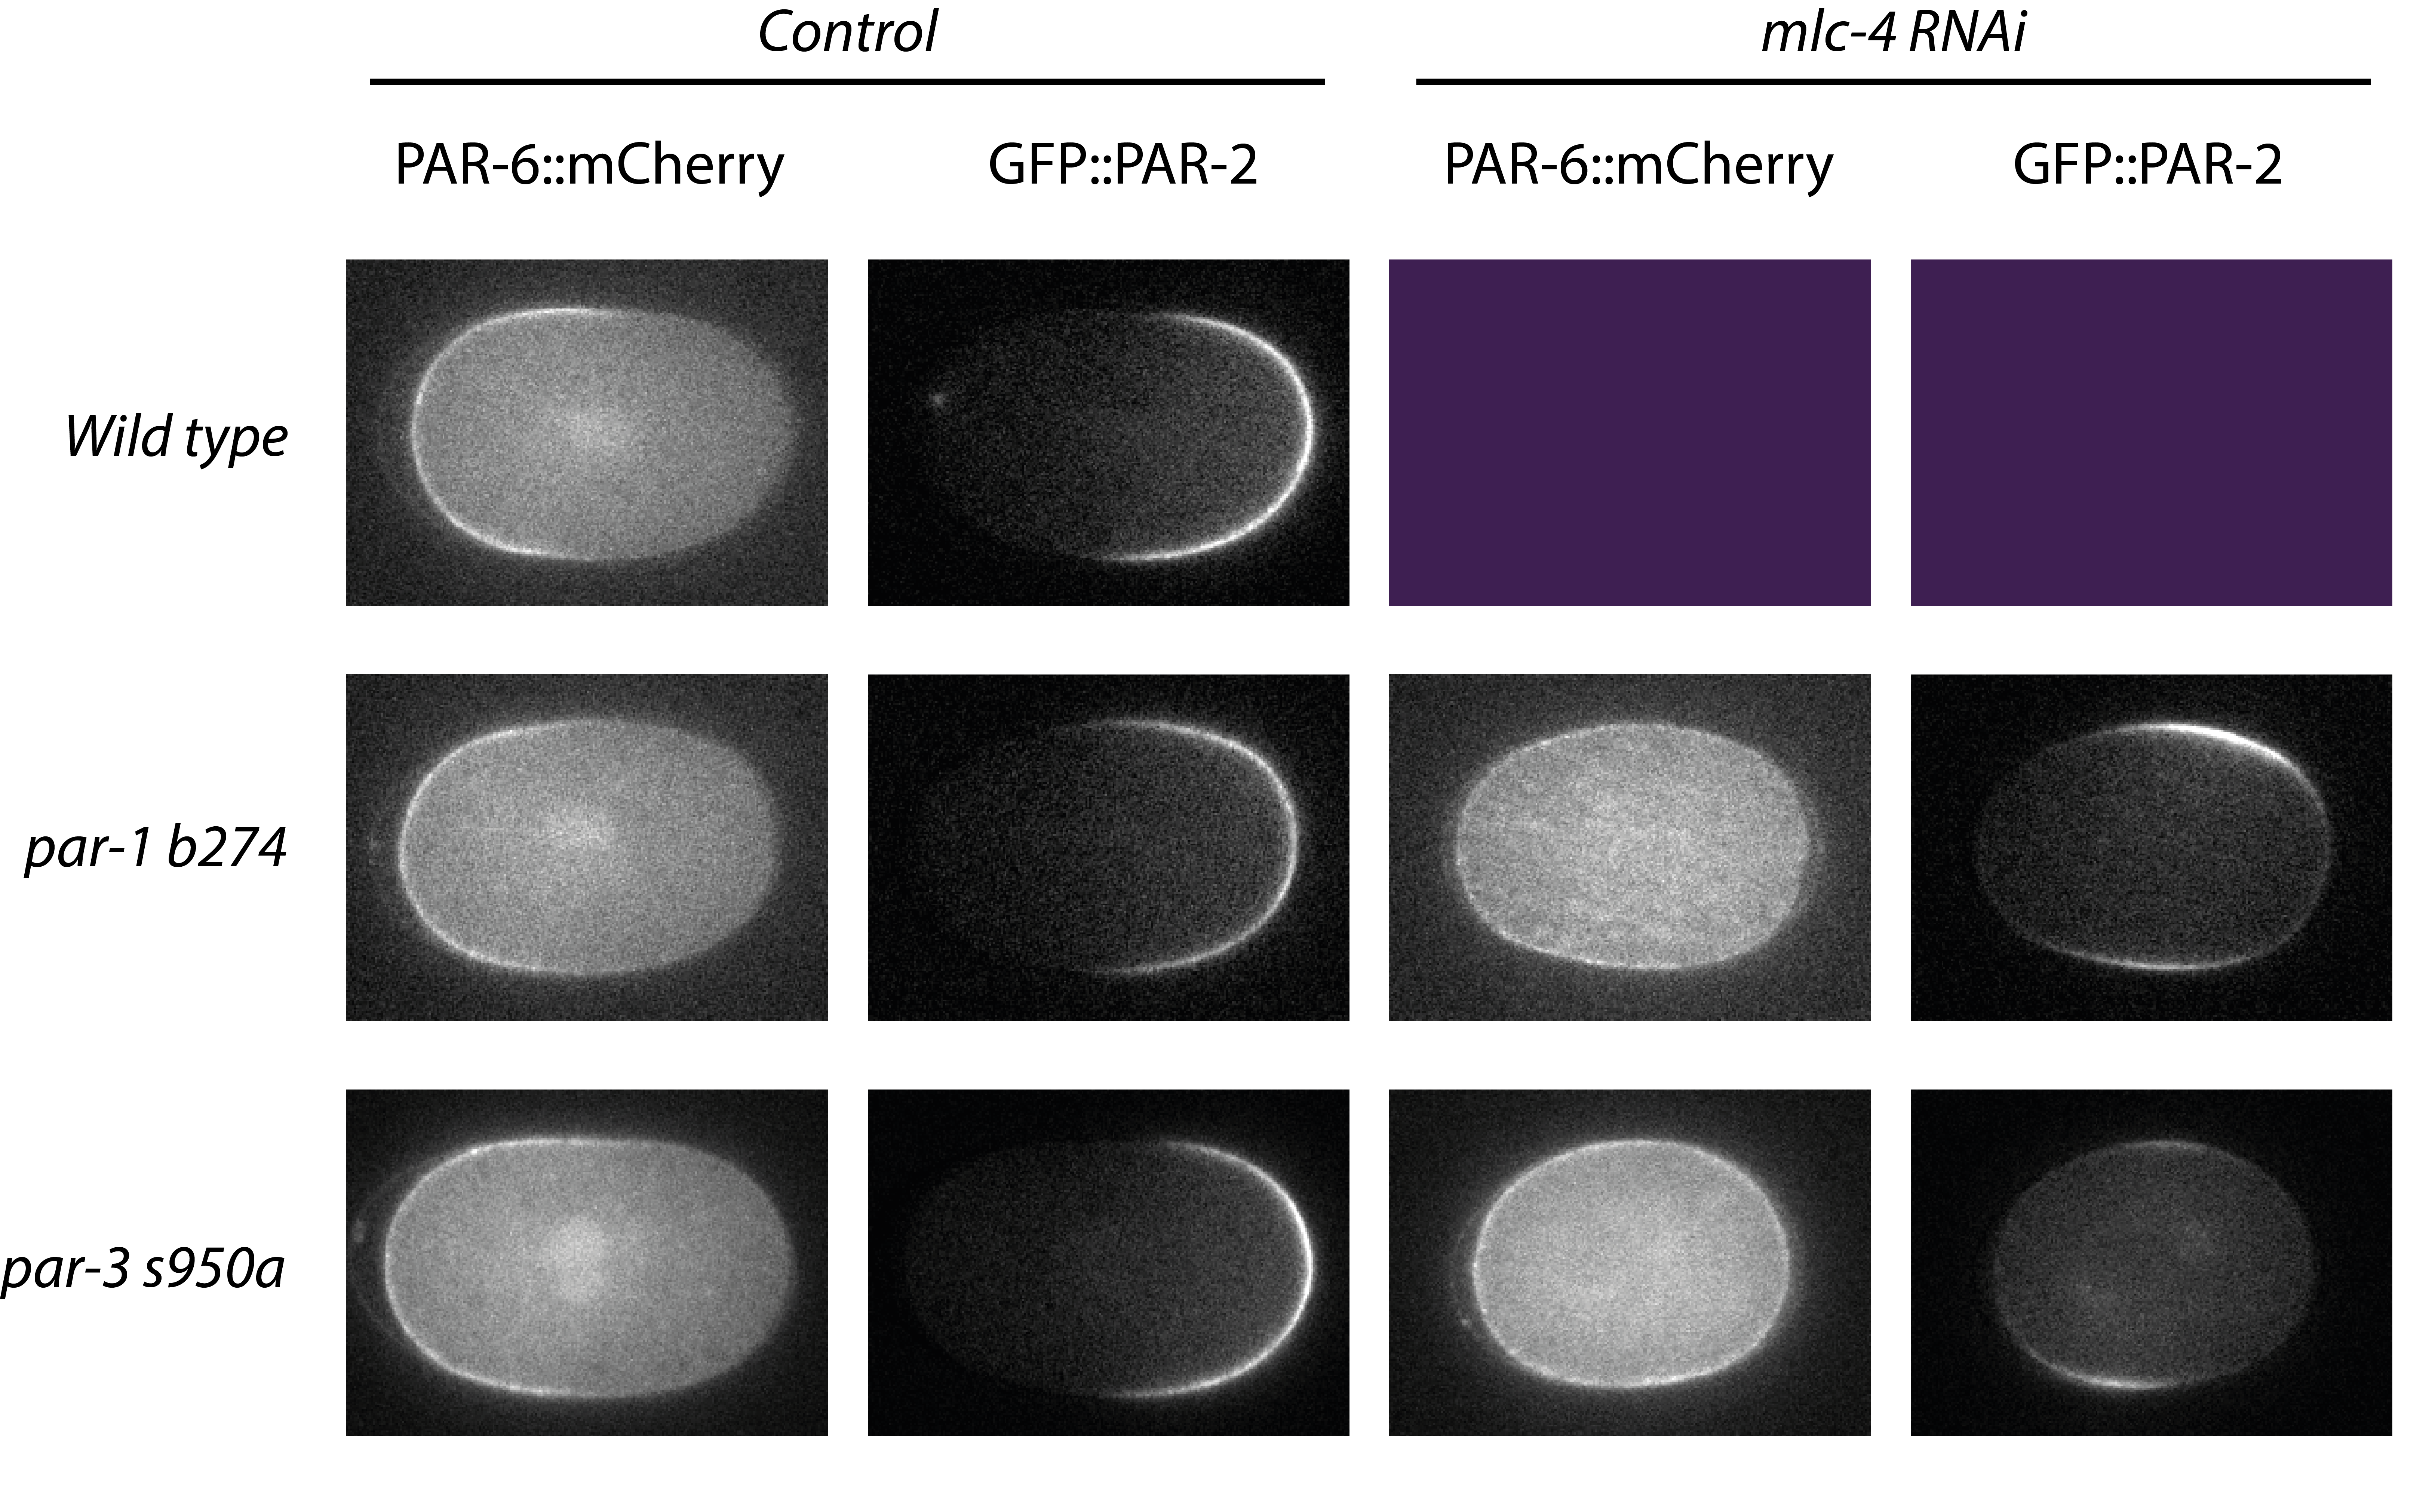
\includegraphics[scale=0.9]{uniform_polarity}
\setlength{\abovecaptionskip}{20pt}
\centering
\mycaption{Title}{Caption}
\label{fig:uniform_polarity}
\end{figure}

\clearpage
\subsection{Symmetry breaking against uniform aPAR}

\begin{figure}[!h]
\includegraphics[scale=0.9]{uniform_polarity_sb}
\setlength{\abovecaptionskip}{20pt}
\centering
\mycaption{Title}{Caption}
\label{fig:uniform_polarity_sb}
\end{figure}

\clearpage
\subsection{Polarity phenotypes in PAR-2 mutants}

\begin{figure}[!h]
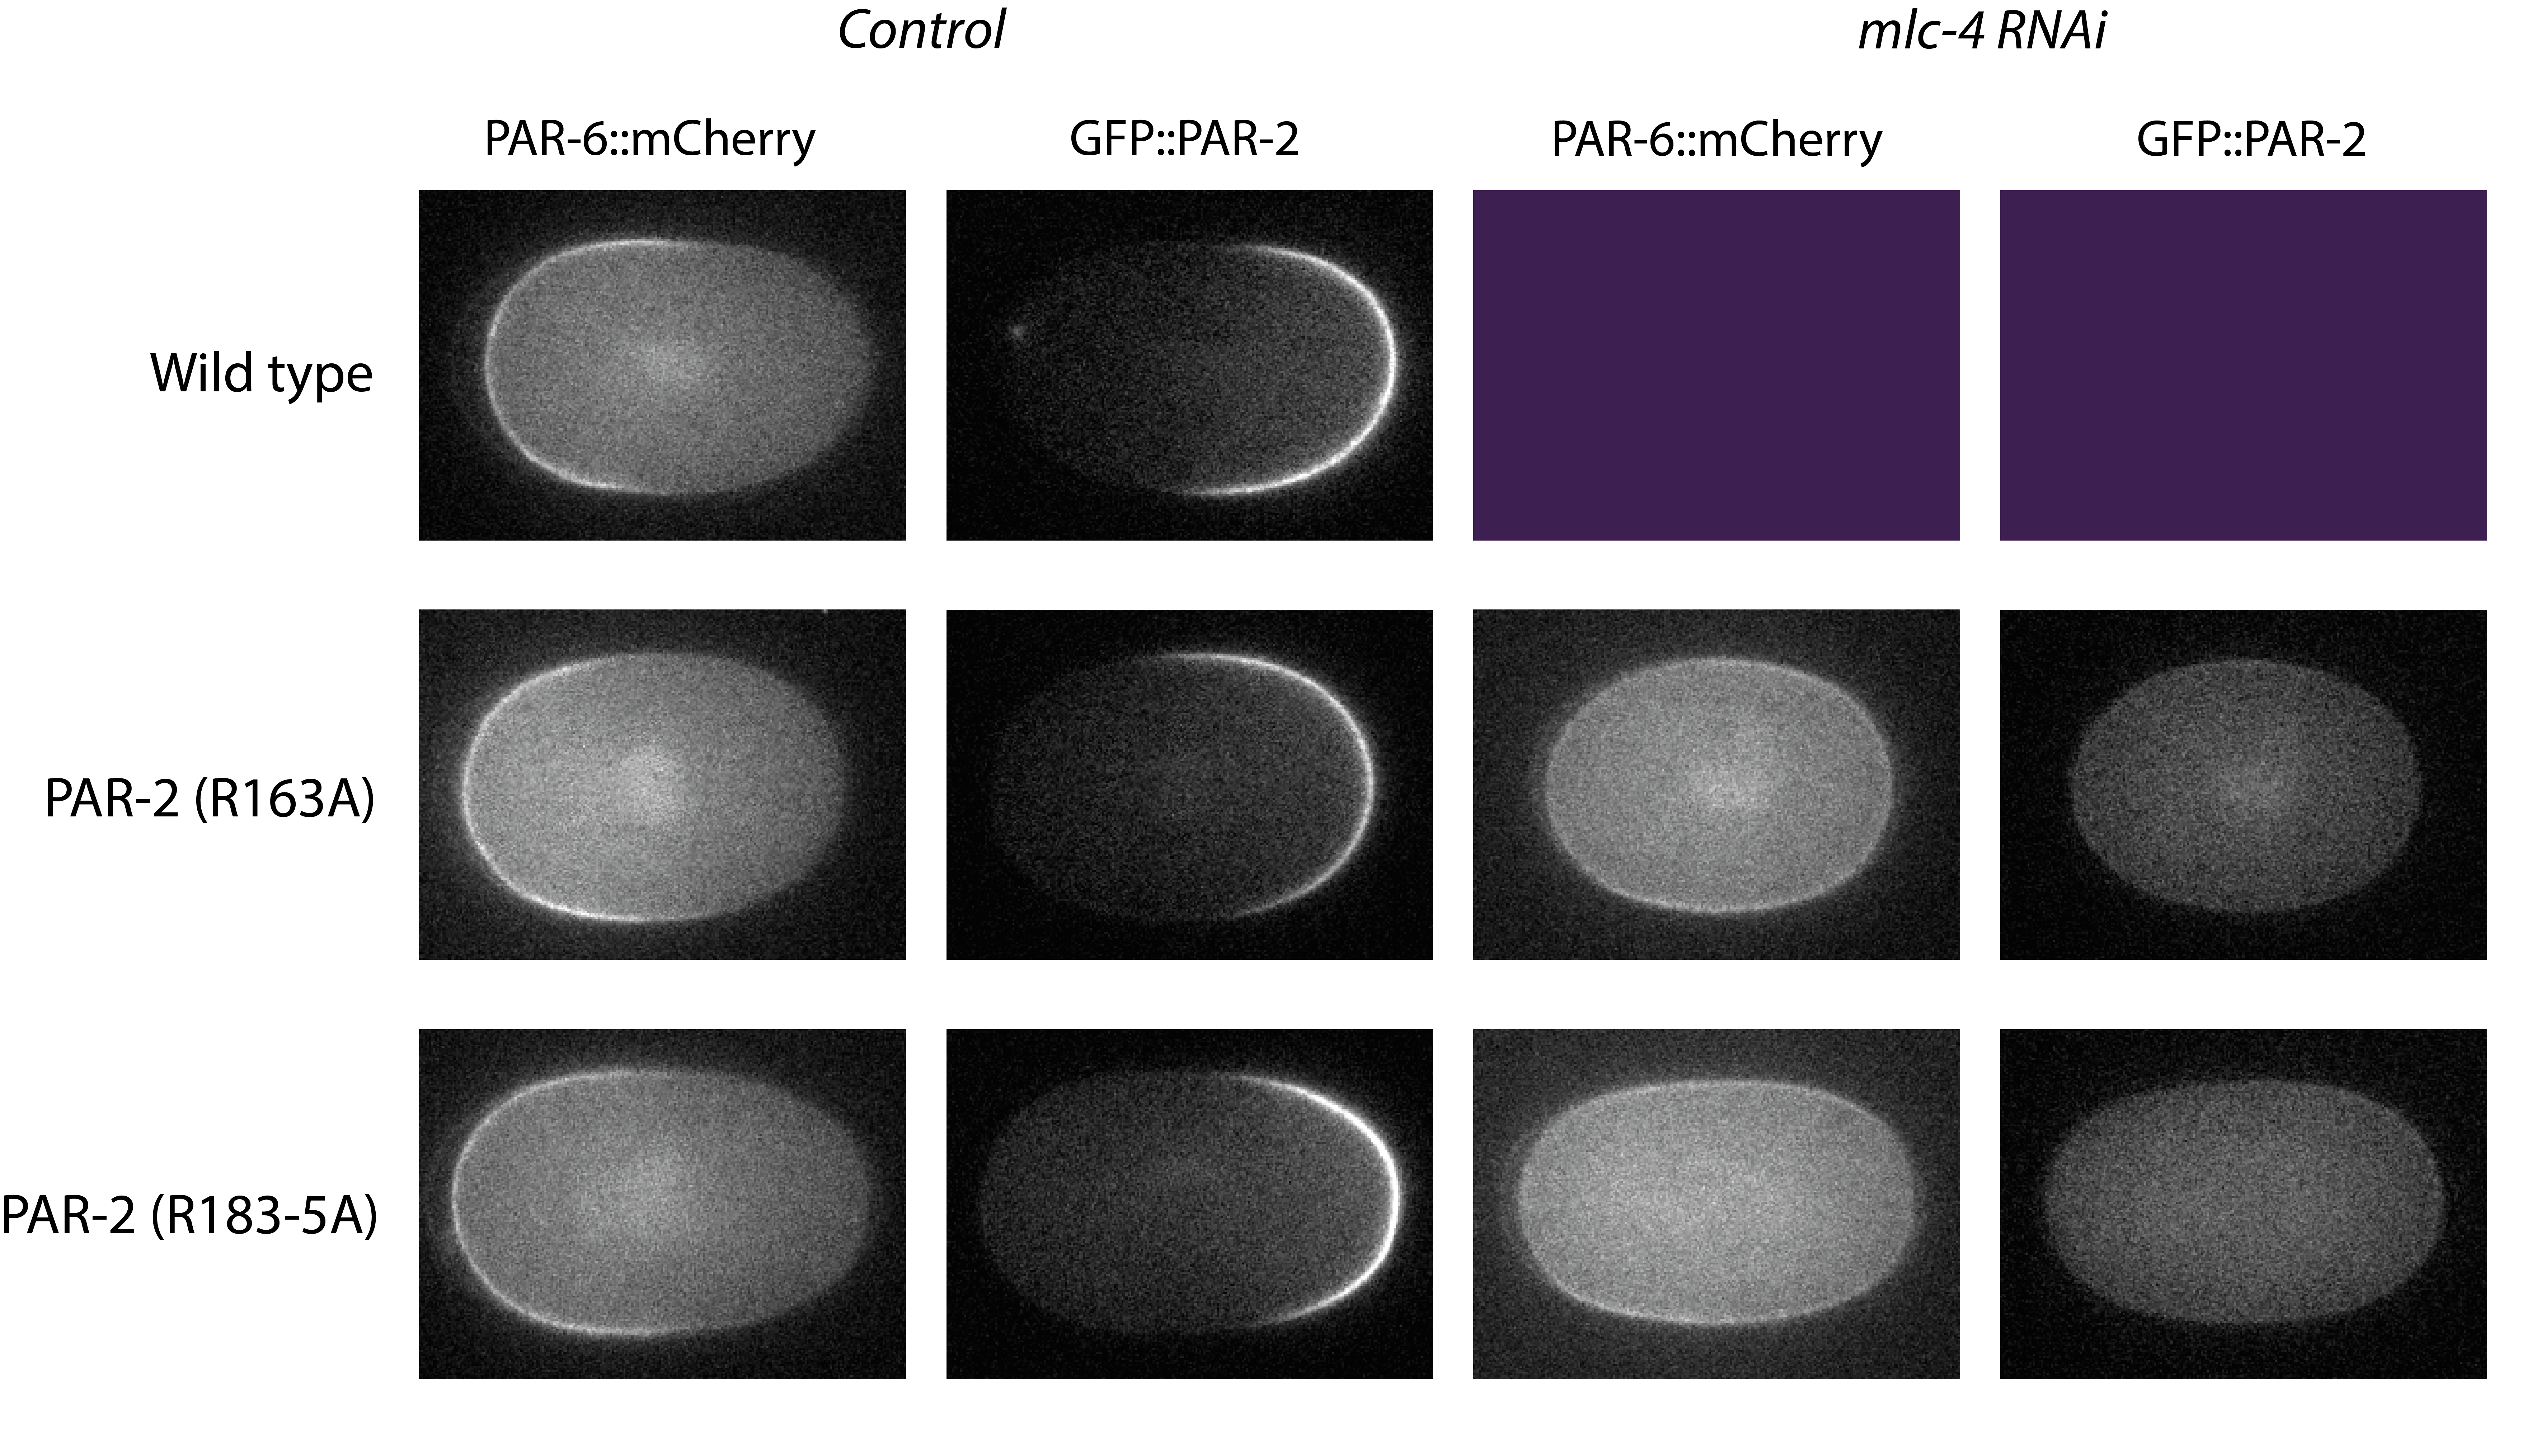
\includegraphics[scale=0.9]{uniform_polarity_mutants}
\setlength{\abovecaptionskip}{20pt}
\centering
\mycaption{Title}{Caption}
\label{fig:uniform_polarity_mutants}
\end{figure}

\clearpage
\subsection{Quantitative characterisation of PAR-2 mutants}

\subsection{Discussion}

%%%%%%%%%%%%%%%%%%%%%%%%%%%%%%%%%%%%%%%%%%%%%%%%%%%%%%%%%%
\clearpage
\section{Determining mechanisms of PAR-2 RING domain action}

% needs to comment on positive feedback more

Since initial observations that RING mutants show weaker membrane association, the RING domain has been widely believed to play an important role in regulating the membrane affinity of the protein. However, the precise role carried out by the RING domain in this context is not yet understood. On its own, the PAR-2 RING domain in isolation shows no membrane binding activity (Hao, and replicated below). Therefore it's likely that, rather than a direct membrane binding role, the RING domain sets membrane affinity by regulating electrostatic binding via the central charged region of the protein.\\

Given the common role for RING domain proteins as ubiquitin ligases, it's tempting to speculate that ubiquitination activity at the cortex might change the electrostatic profile of the membrane in some way to make it more favourable for PAR-2 binding. However, as has been previously observed (ref), the membrane affinity of C56S PAR-2 is independent on the presence of wild type PAR-2. I have replicated this finding, more quantitatively, in figure x. Here, I show that, for C56S mutant PAR-2, membrane affinity is unchanged when balanced by a wild type copy compared to when homozygous. In other words, the effects of C56S mutation appear to be cis acting, intrinsic to each molecule.

\begin{figure}[!h]
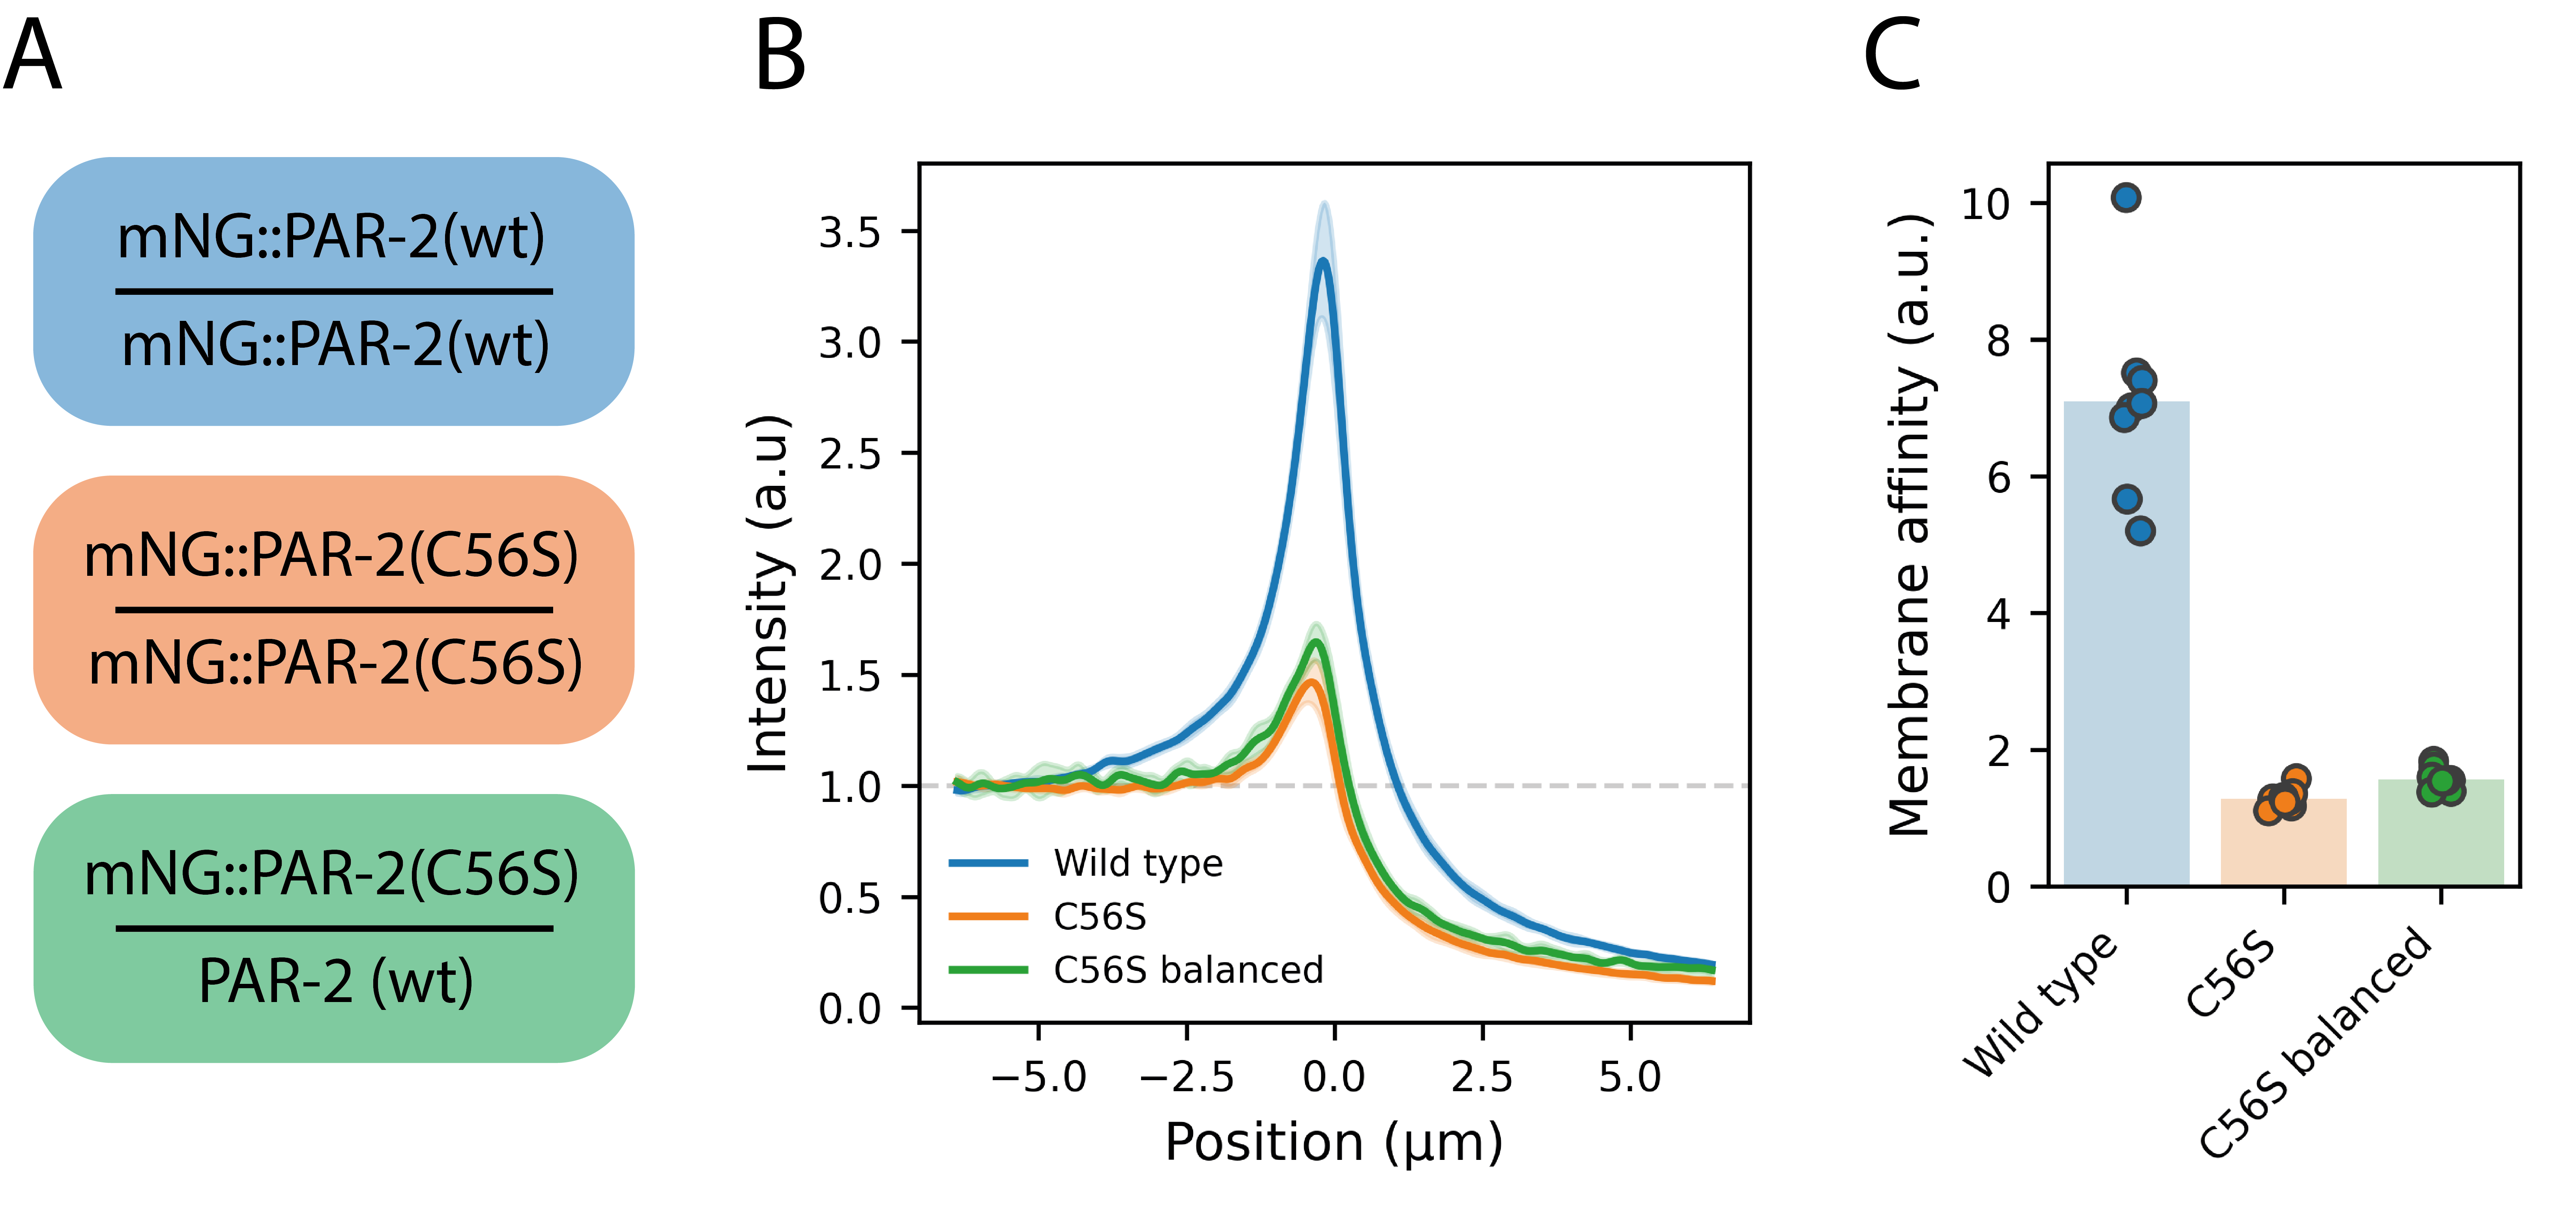
\includegraphics[scale=1]{c56s_cis}
\setlength{\abovecaptionskip}{20pt}
\centering
\mycaption{Title}{Caption}
\label{fig:c56s_cis}
\end{figure}

With this in mind, the potential models for RING domain action are greatly limited. We could not, for example, have a scenario whereby PAR-2 is ubiquitinating some membrane target to make the membrane environment more favourable for membrane binding, as such a mechanism would mean that C56S mutant PAR-2 should be responsive to the presence of wild type PAR-2. I therefore believe that there are two, not mutually exclusive, possibilities, which I aim to explore in this section:
\begin{enumerate}
\item The RING domain regulates PAR-2 membrane affinity through autoubiquitination, perhaps to sites within the membrane binding domain
\item The RING domain promotes dimerisation of PAR-2, leading to enhanced membrane affinity
\end{enumerate}

A third possibility, which I will touch upon but do not directly investigate, is that, rather than functional RING having a positive effect on membrane binding, the unfolded RING domain in the C56S mutant may directly interfere with normal electrostatic membrane binding.

\subsection{Exploring a role for ubiquitination}

\textit{This section describes work performed with Colin Davis in Anne Schreiber's lab, and Diego Esposito in Katrin Rittinger's lab, both at the Crick}

\subsubsection{PAR-2 purification and in vitro ubiquitination assays}

% Shown to interact with E2 enzymes in yeast two hybrid assays

% Whilst the Hao paper reports unpublished data

We expressed strep-tagged full-length PAR-2 in insect cells, lysed cells by sonication, and purified by pull-down followed by size exclusion chromatography (see Methods). From the initial pull-down stage, we observed two prominant bands close to the expected mass of PAR-2. Due to their similar masess, we were unable to separate the two bands by size exclusion chromatography (fig x). We tested both bands by mass spectrometry, which confirmed them both to be PAR-2. Interestingly, a single ubiquitinated site (K...) was identified in the upper band sample, explaining the higher mass. No ubiquitinated sites were found in the lower band sample, although the K... site was not covered. We also observed similar bands in a small-scale prep of C56S mutant PAR-2. Therefore, I do not believe this to be a result of autoubiquitination, but may rather represent ubiquitination of the protein by an insect E3 within the insect cell. CRISPR mutation of K... has no effect in vivo (data not shown), and attempts to purify PAR-2 from worm lysates and HEK cell preps have not shown two bands.\\

% Sample from SEC purification was pooled (lanes x-x)

% Whereas the positive control sample (TRIM2) showed rapid auto-polyubiquitination and depletion of ubiquitin within 30 minutes, no effect was observed for PAR-2 across the whole 60 minutes of the experiment, indicating lack of ubiquitniation activity.

\begin{figure}[!h]
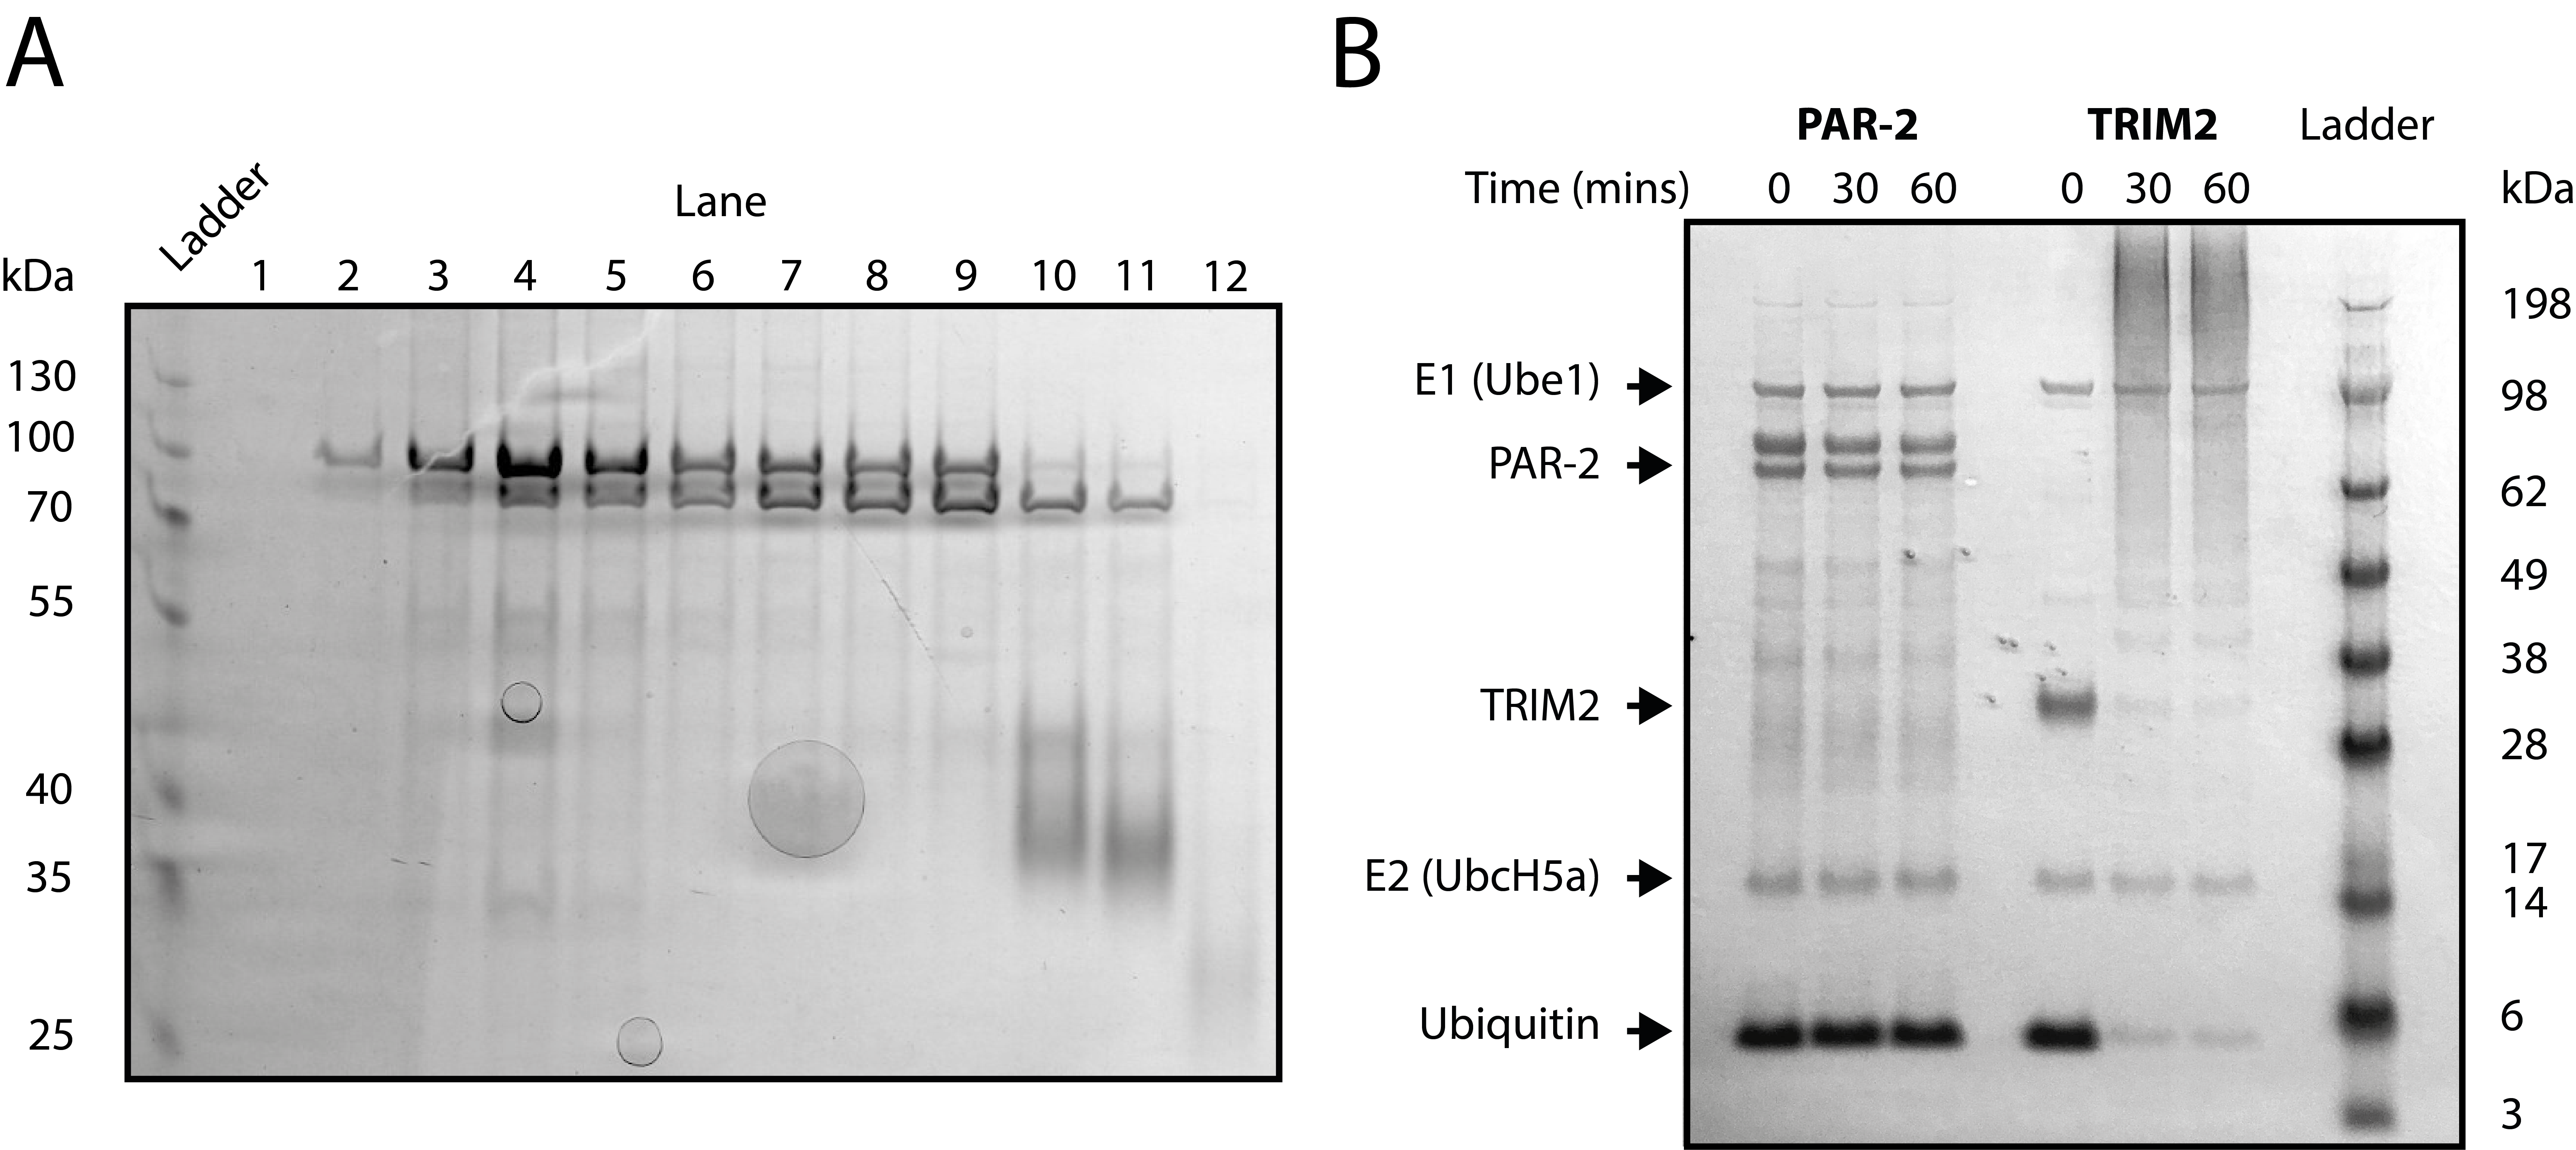
\includegraphics[scale=1]{ubiquitin_assay}
\setlength{\abovecaptionskip}{20pt}
\centering
\mycaption{Title}{Caption}
\label{ubiquitin_assay}
\end{figure}



\clearpage
\subsubsection{Targeted mutation to putative linchpin site}

A key site in many RING E3 ligases is an arginine or lysine residue immediately downstream of the final zinc-coordinating cysteine, which is known as the linchpin site. <what does this site do?>. 46\% of RING domains have an arginine at this site linchpin, whereas 14\% have lysine \citep{Stewart2017}. Typically, the choice of residue at this site regulates a trade-off between ubiquitination activity and E2 specificity. RINGs with a K at this site typically show lower ubiquitination activity in vitro (REF). Stewart showed for the protein <> that mutating this site from an arginine to a lysine increases ubiquitination activity but reduces E2 specificity (CHECK). However, this isn’t a universal mechanism, and many functional RING E3 ligases have other residues at this site <examples, refs>. This suggests that other mechanisms of <> must exist. Currently this is poorly understood.\\

Notably, however, C elegans does have a lysine at this site, suggesting a potential role as a linchpin. Alignment of Caenorhabditis PAR-2 RING domain sequences shows that this site is largely conserved as a lysine (fig x). There are, however, a few exceptions in some of the more distantly related (?) species. C. bovis, castelli and monodelphis have neither an arginine nor a lysine at this site. The fact that this site isn’t universally conserved may argue against an important role for ubiquitination activity, could suggest that PAR-2 does play an role as a ubiquitin ligase but doesn’t rely on the linchpin, or could suggest that these other species have evolved alternative strategies.\\ 

\begin{figure}[!h]
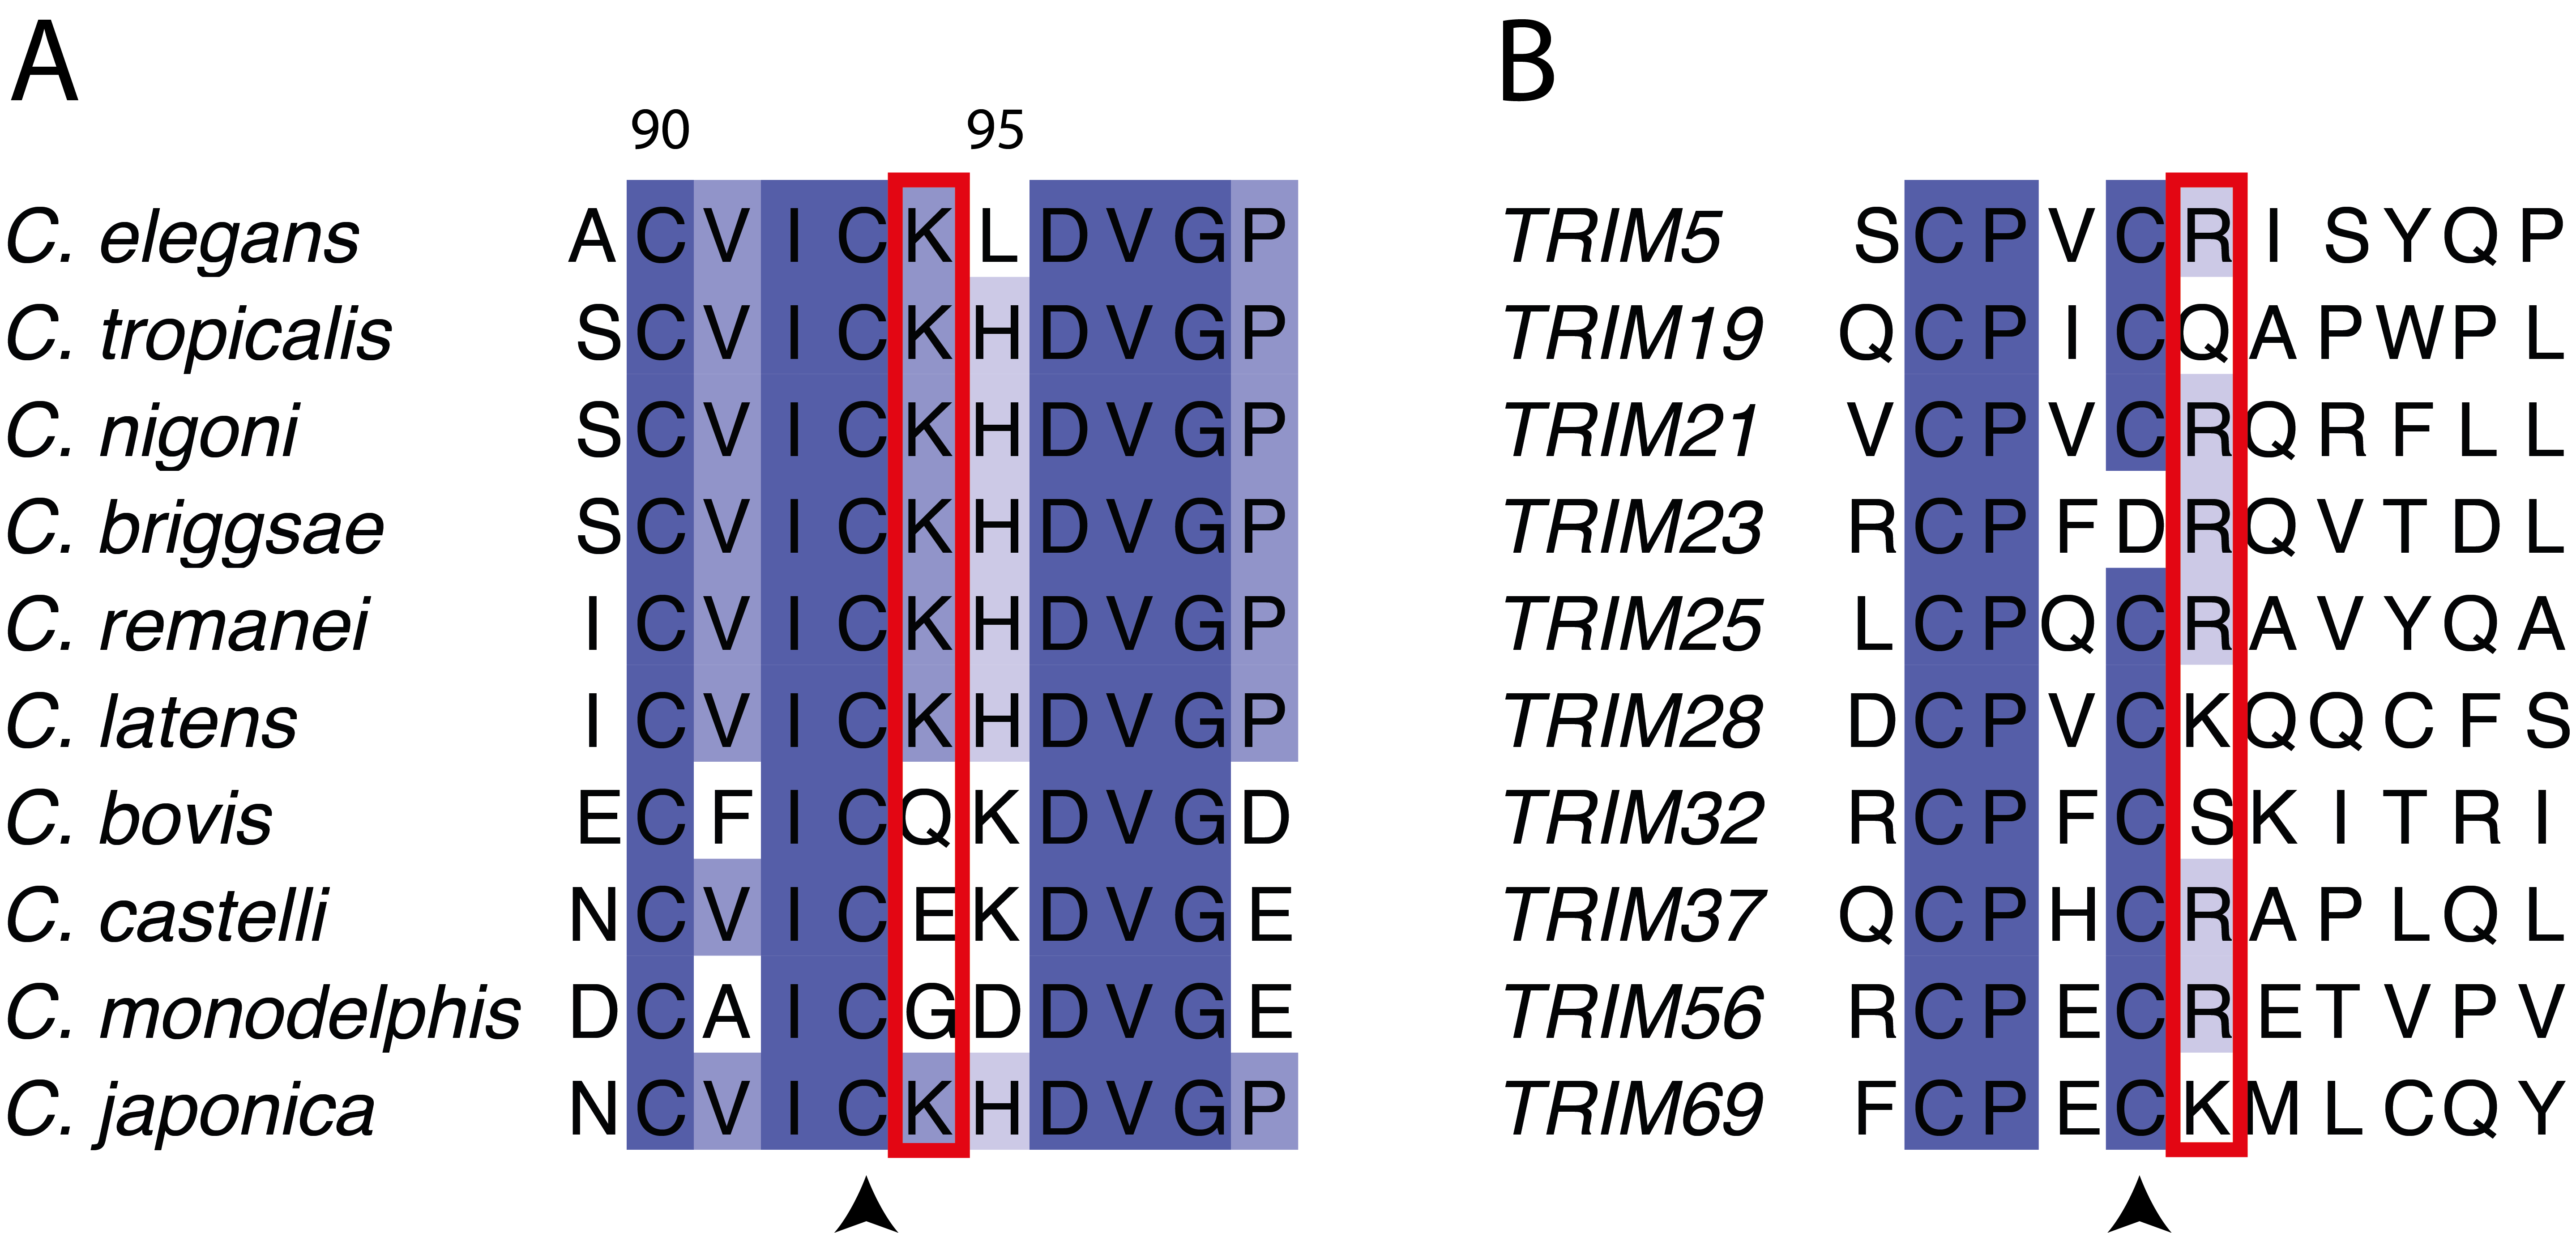
\includegraphics[scale=0.9]{linchpin_alignments}
\setlength{\abovecaptionskip}{20pt}
\centering
\mycaption{Title}{Caption}
\label{fig:linchpin_alignments}
\end{figure}

To test the potential role of linchpin-mediated autoubiquitination for PAR-2 membrane binding affinity, I used CRISPR to perform targeted mutation to this site, turning it into an A. <similar approach used in other studies>. As shown in fig x, this has no detectable effect on membrane affinity. Whilst this cannot rule out a role for ubiquitination in vivo, the result argues against a model in which linchpin-mediated autoubiquitination is a driver of membrane affinity. \\


\begin{figure}[!h]
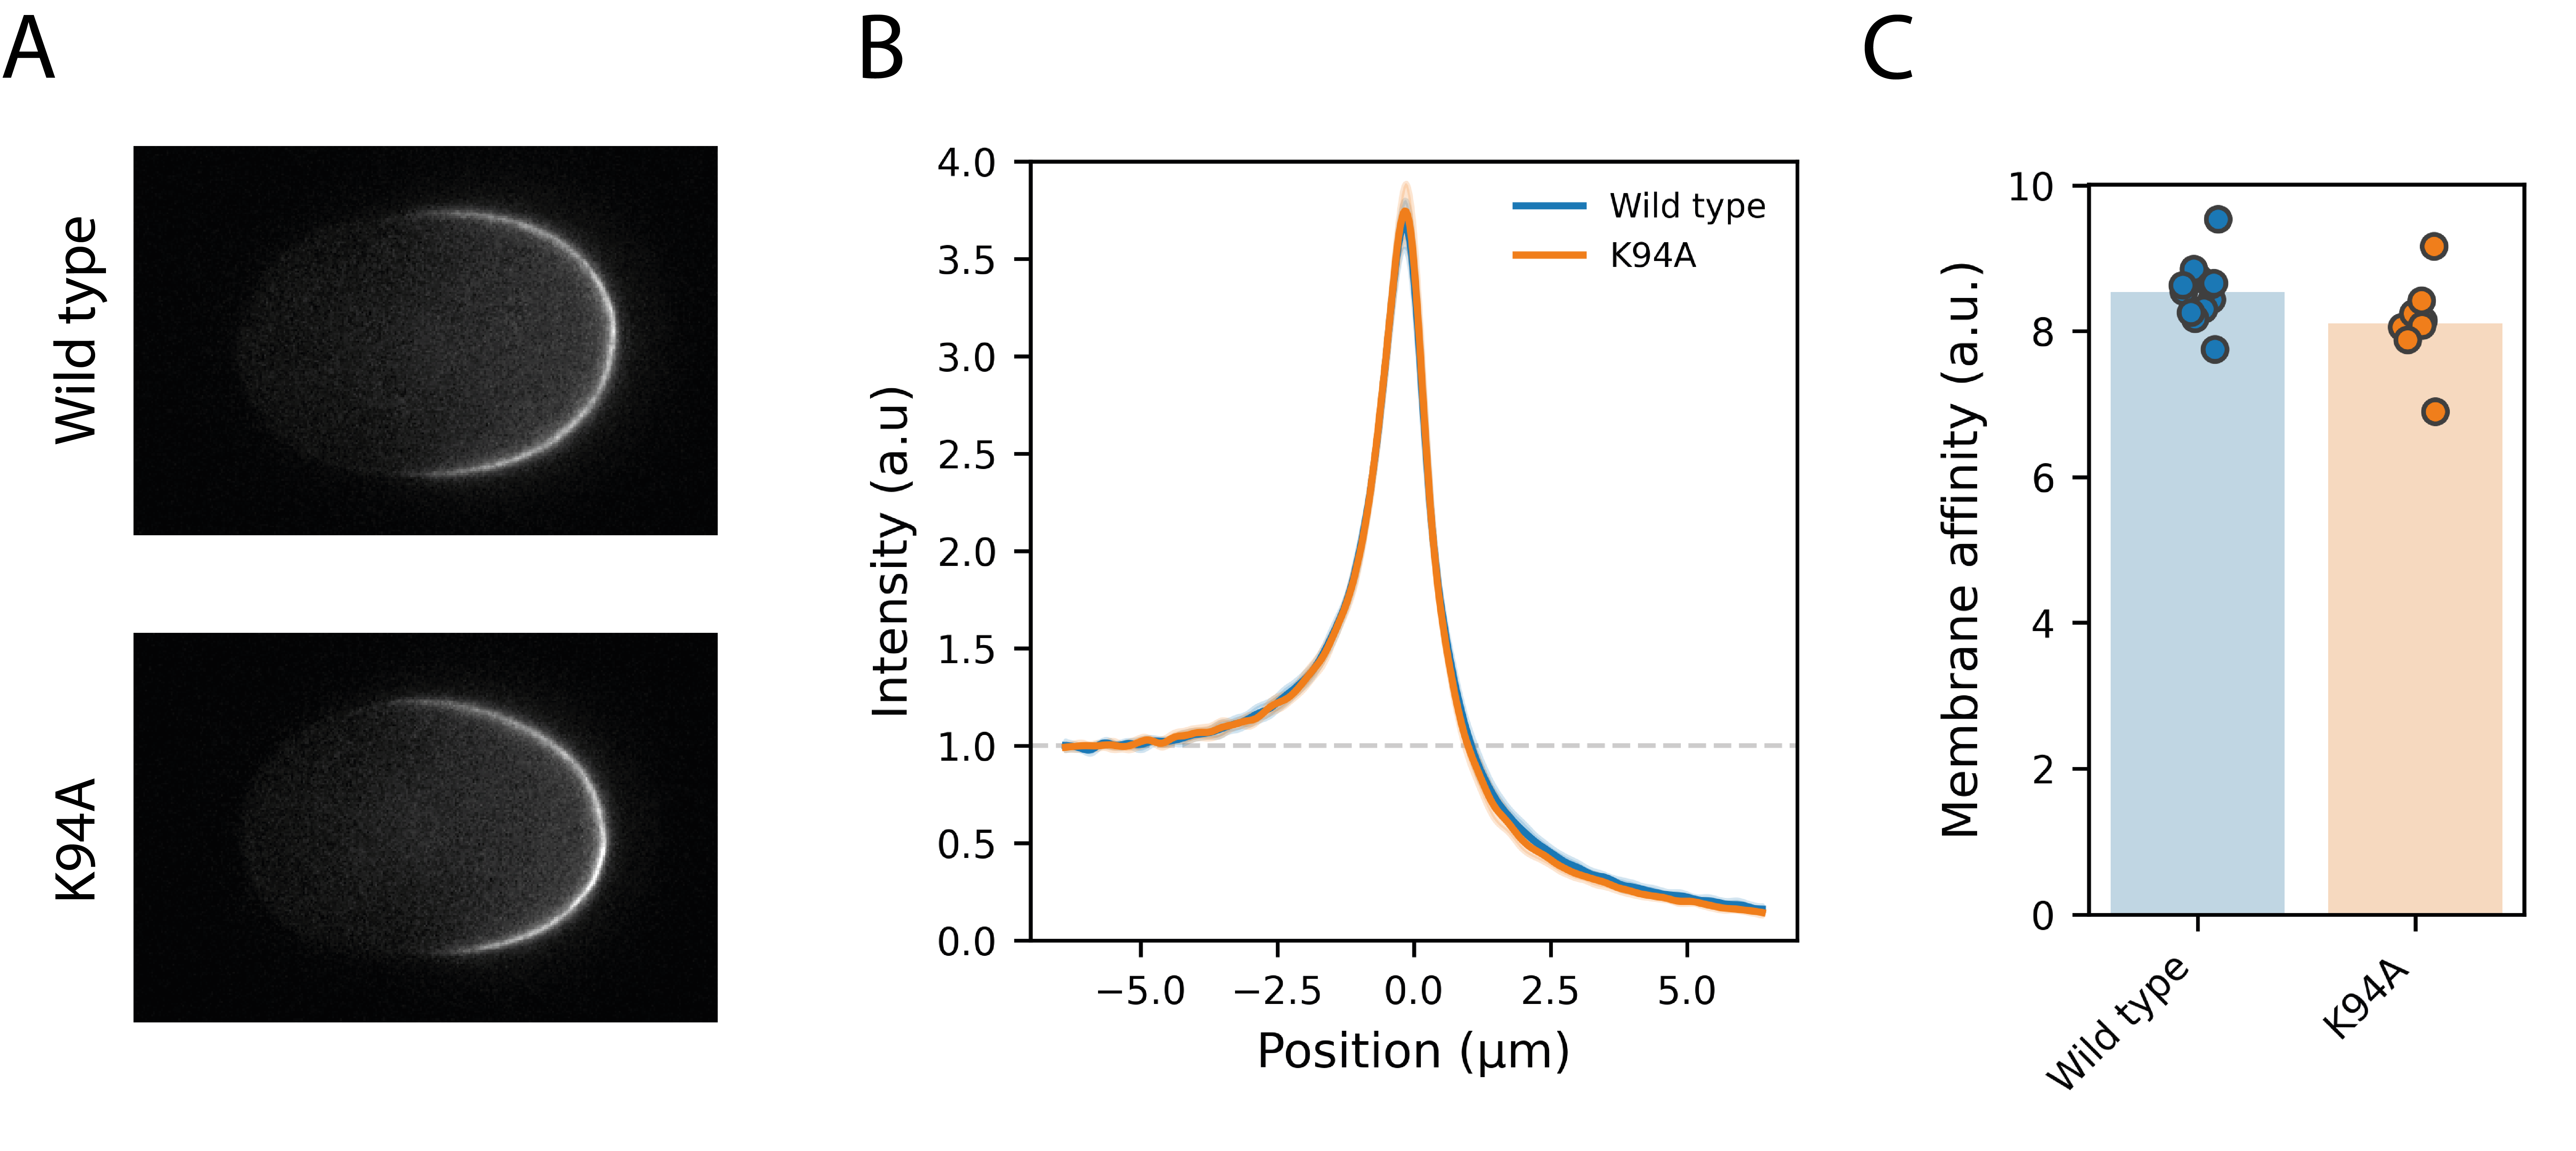
\includegraphics[scale=0.9]{linchpin_in_vivo}
\setlength{\abovecaptionskip}{20pt}
\centering
\mycaption{Title}{Caption}
\label{fig:linchpin_in_vivo}
\end{figure}

\subsubsection{Discussion}

\clearpage
\subsection{Exploring a role for dimerisation}

\subsubsection{RING domain sequence analysis}

As a first step, I performed a BLAST search to compare the PAR-2 sequence against sequences for which the quaternary structure has been solved using laboratory methods, using the online SWISS model tool. This yielded hits for a number of well-characterised RING domains, most of which are dimeric in their crystal structures (table x). RING domain dimerisation is typically mediated by a four-helix bundle, consisting of short alpha-helical segments N- and C- terminal to the core RING domain each of the two monomers. By forming a hydrophobic interface, dimerisation is stabilised. Thus, dimeric RING domains have a characteristic pattern of hydrophobic residues in the regions upstream and downstream of the core RING domain. Sequence alignment shows that, whilst the precise pattern of hydrophobic varies slightly between different proteins, PAR-2 follows the general pattern expected of dimeric RING domains (fig x).\\

\begin{figure}[!h]
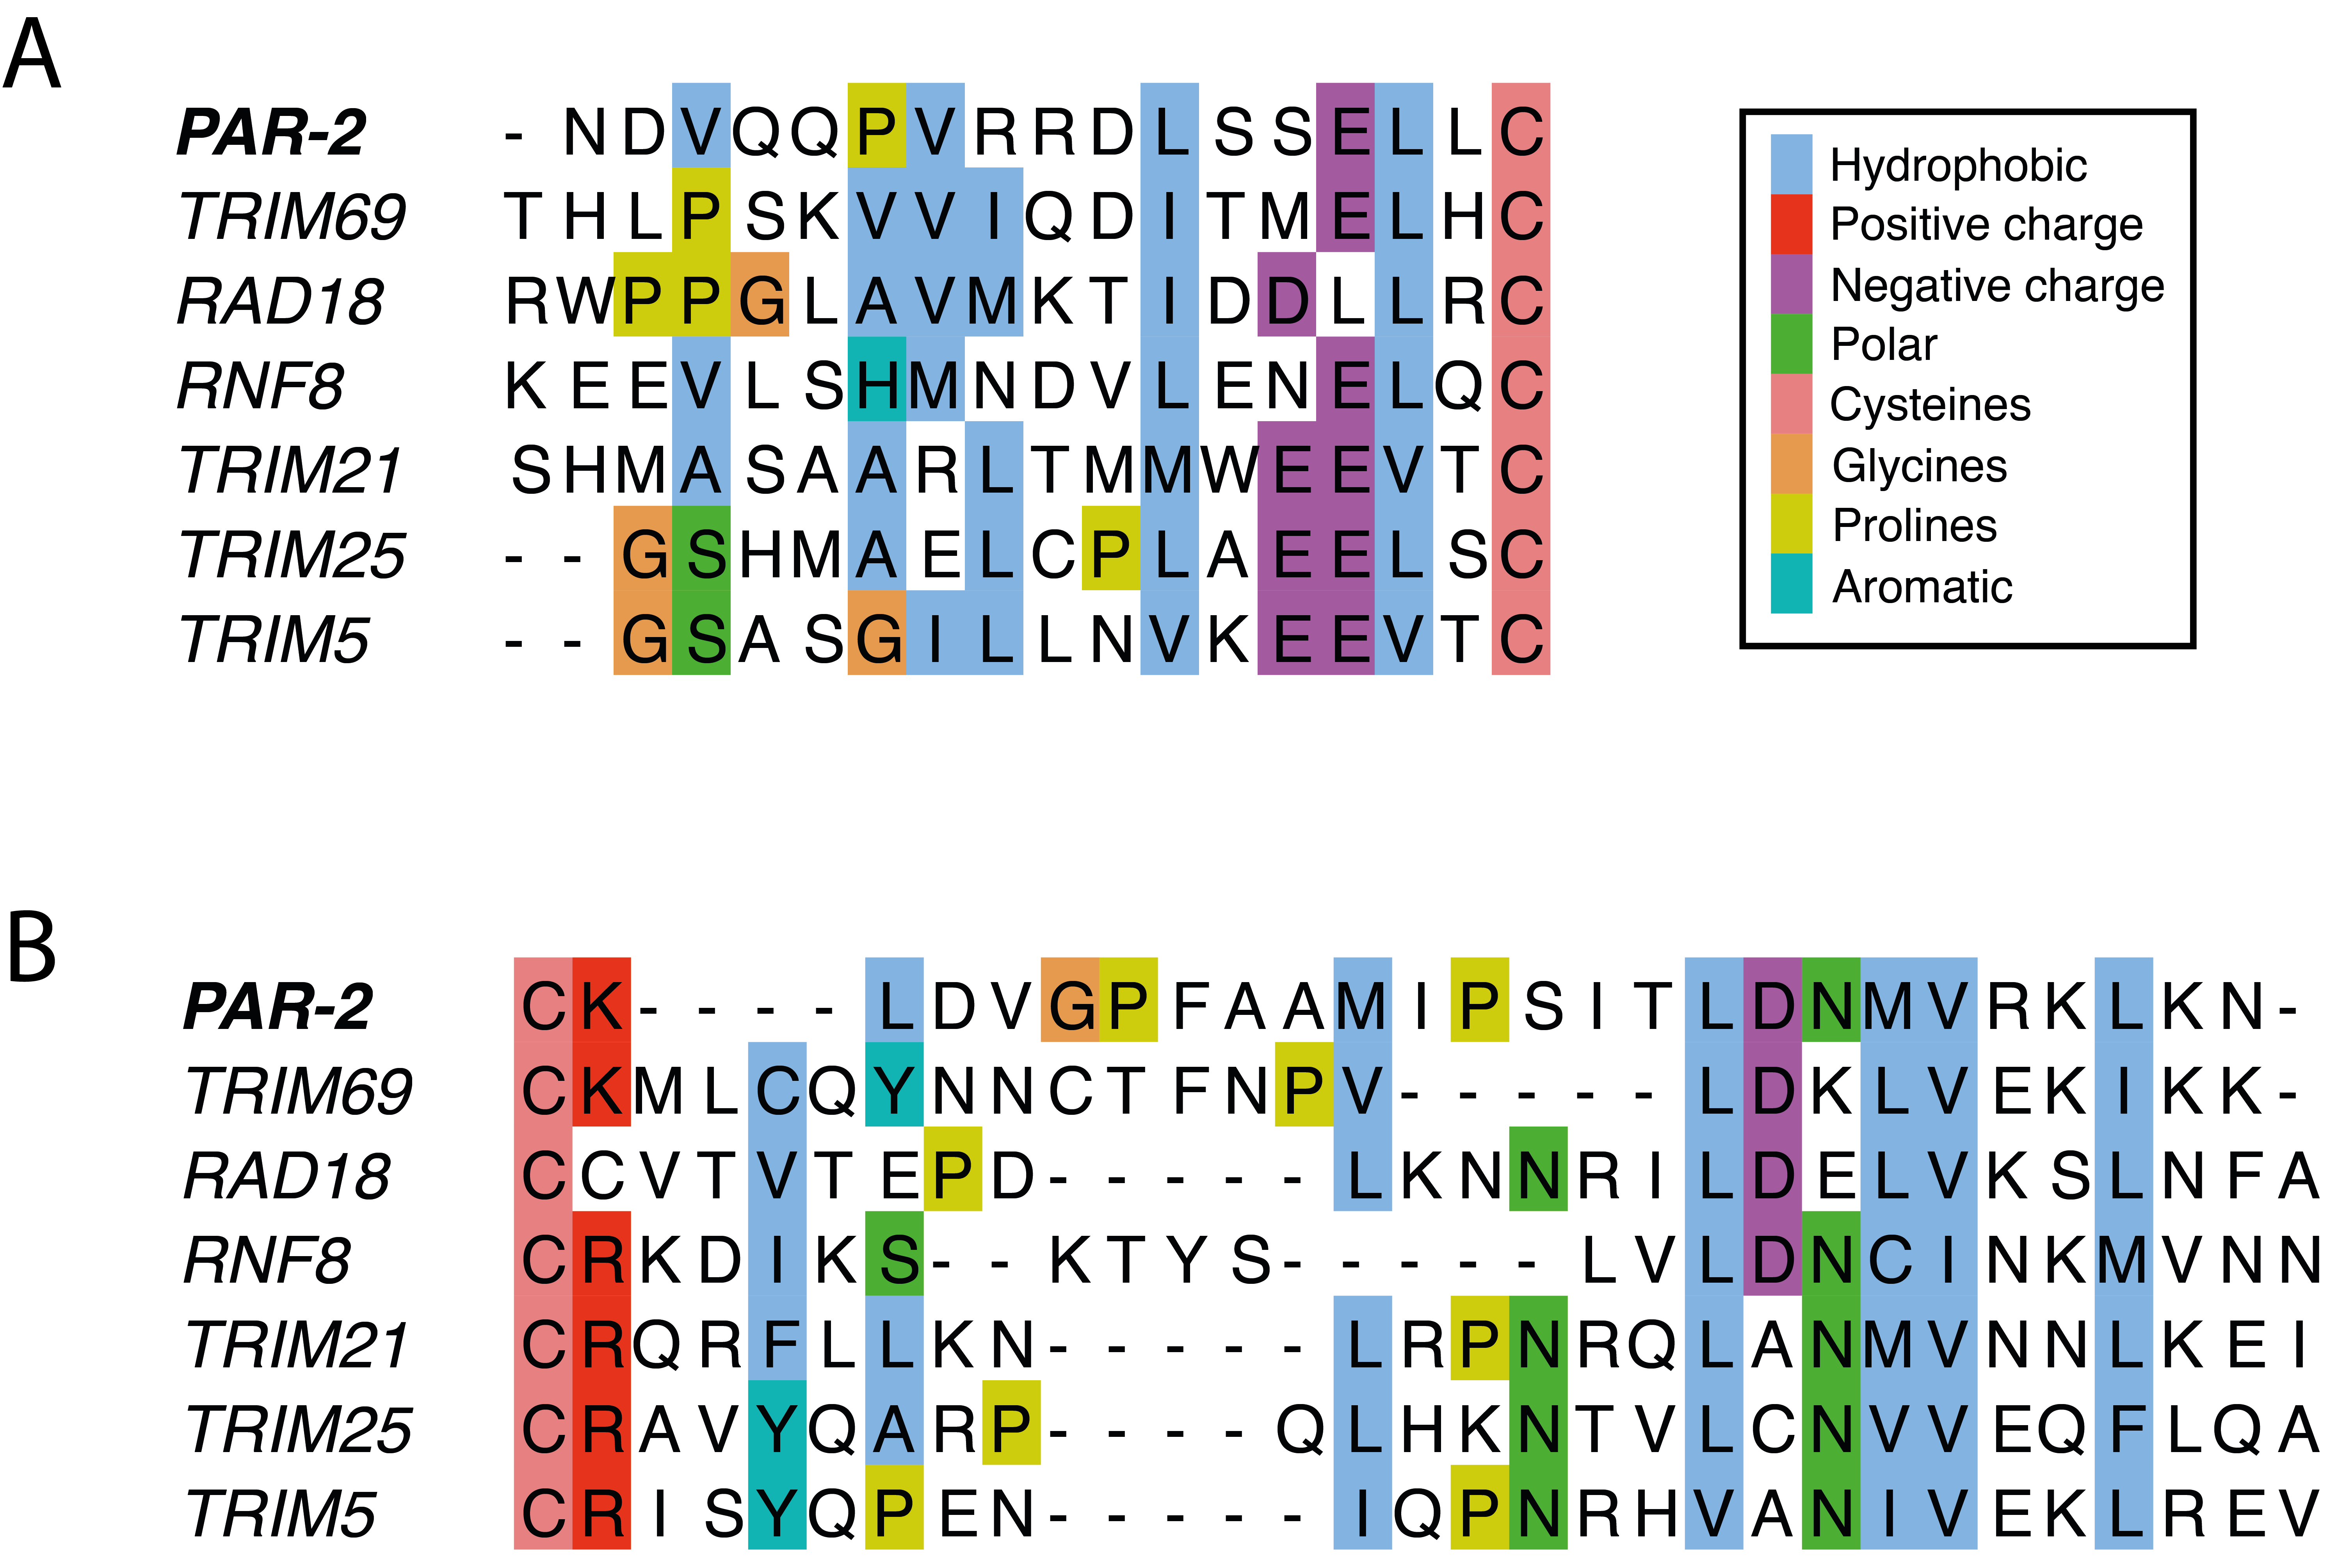
\includegraphics[scale=1]{alignments_other_rings}
\setlength{\abovecaptionskip}{20pt}
\centering
\mycaption{Title}{Caption}
\label{fig:alignments_other_rings}
\end{figure}

As shown in fig x, these regions are highly conserved in different Caenorhabditis species. Most species show an identical pattern of hydrophobic residues, which points to a potentially important role for PAR-2 RING domain dimerisation. \\

\begin{figure}[!h]
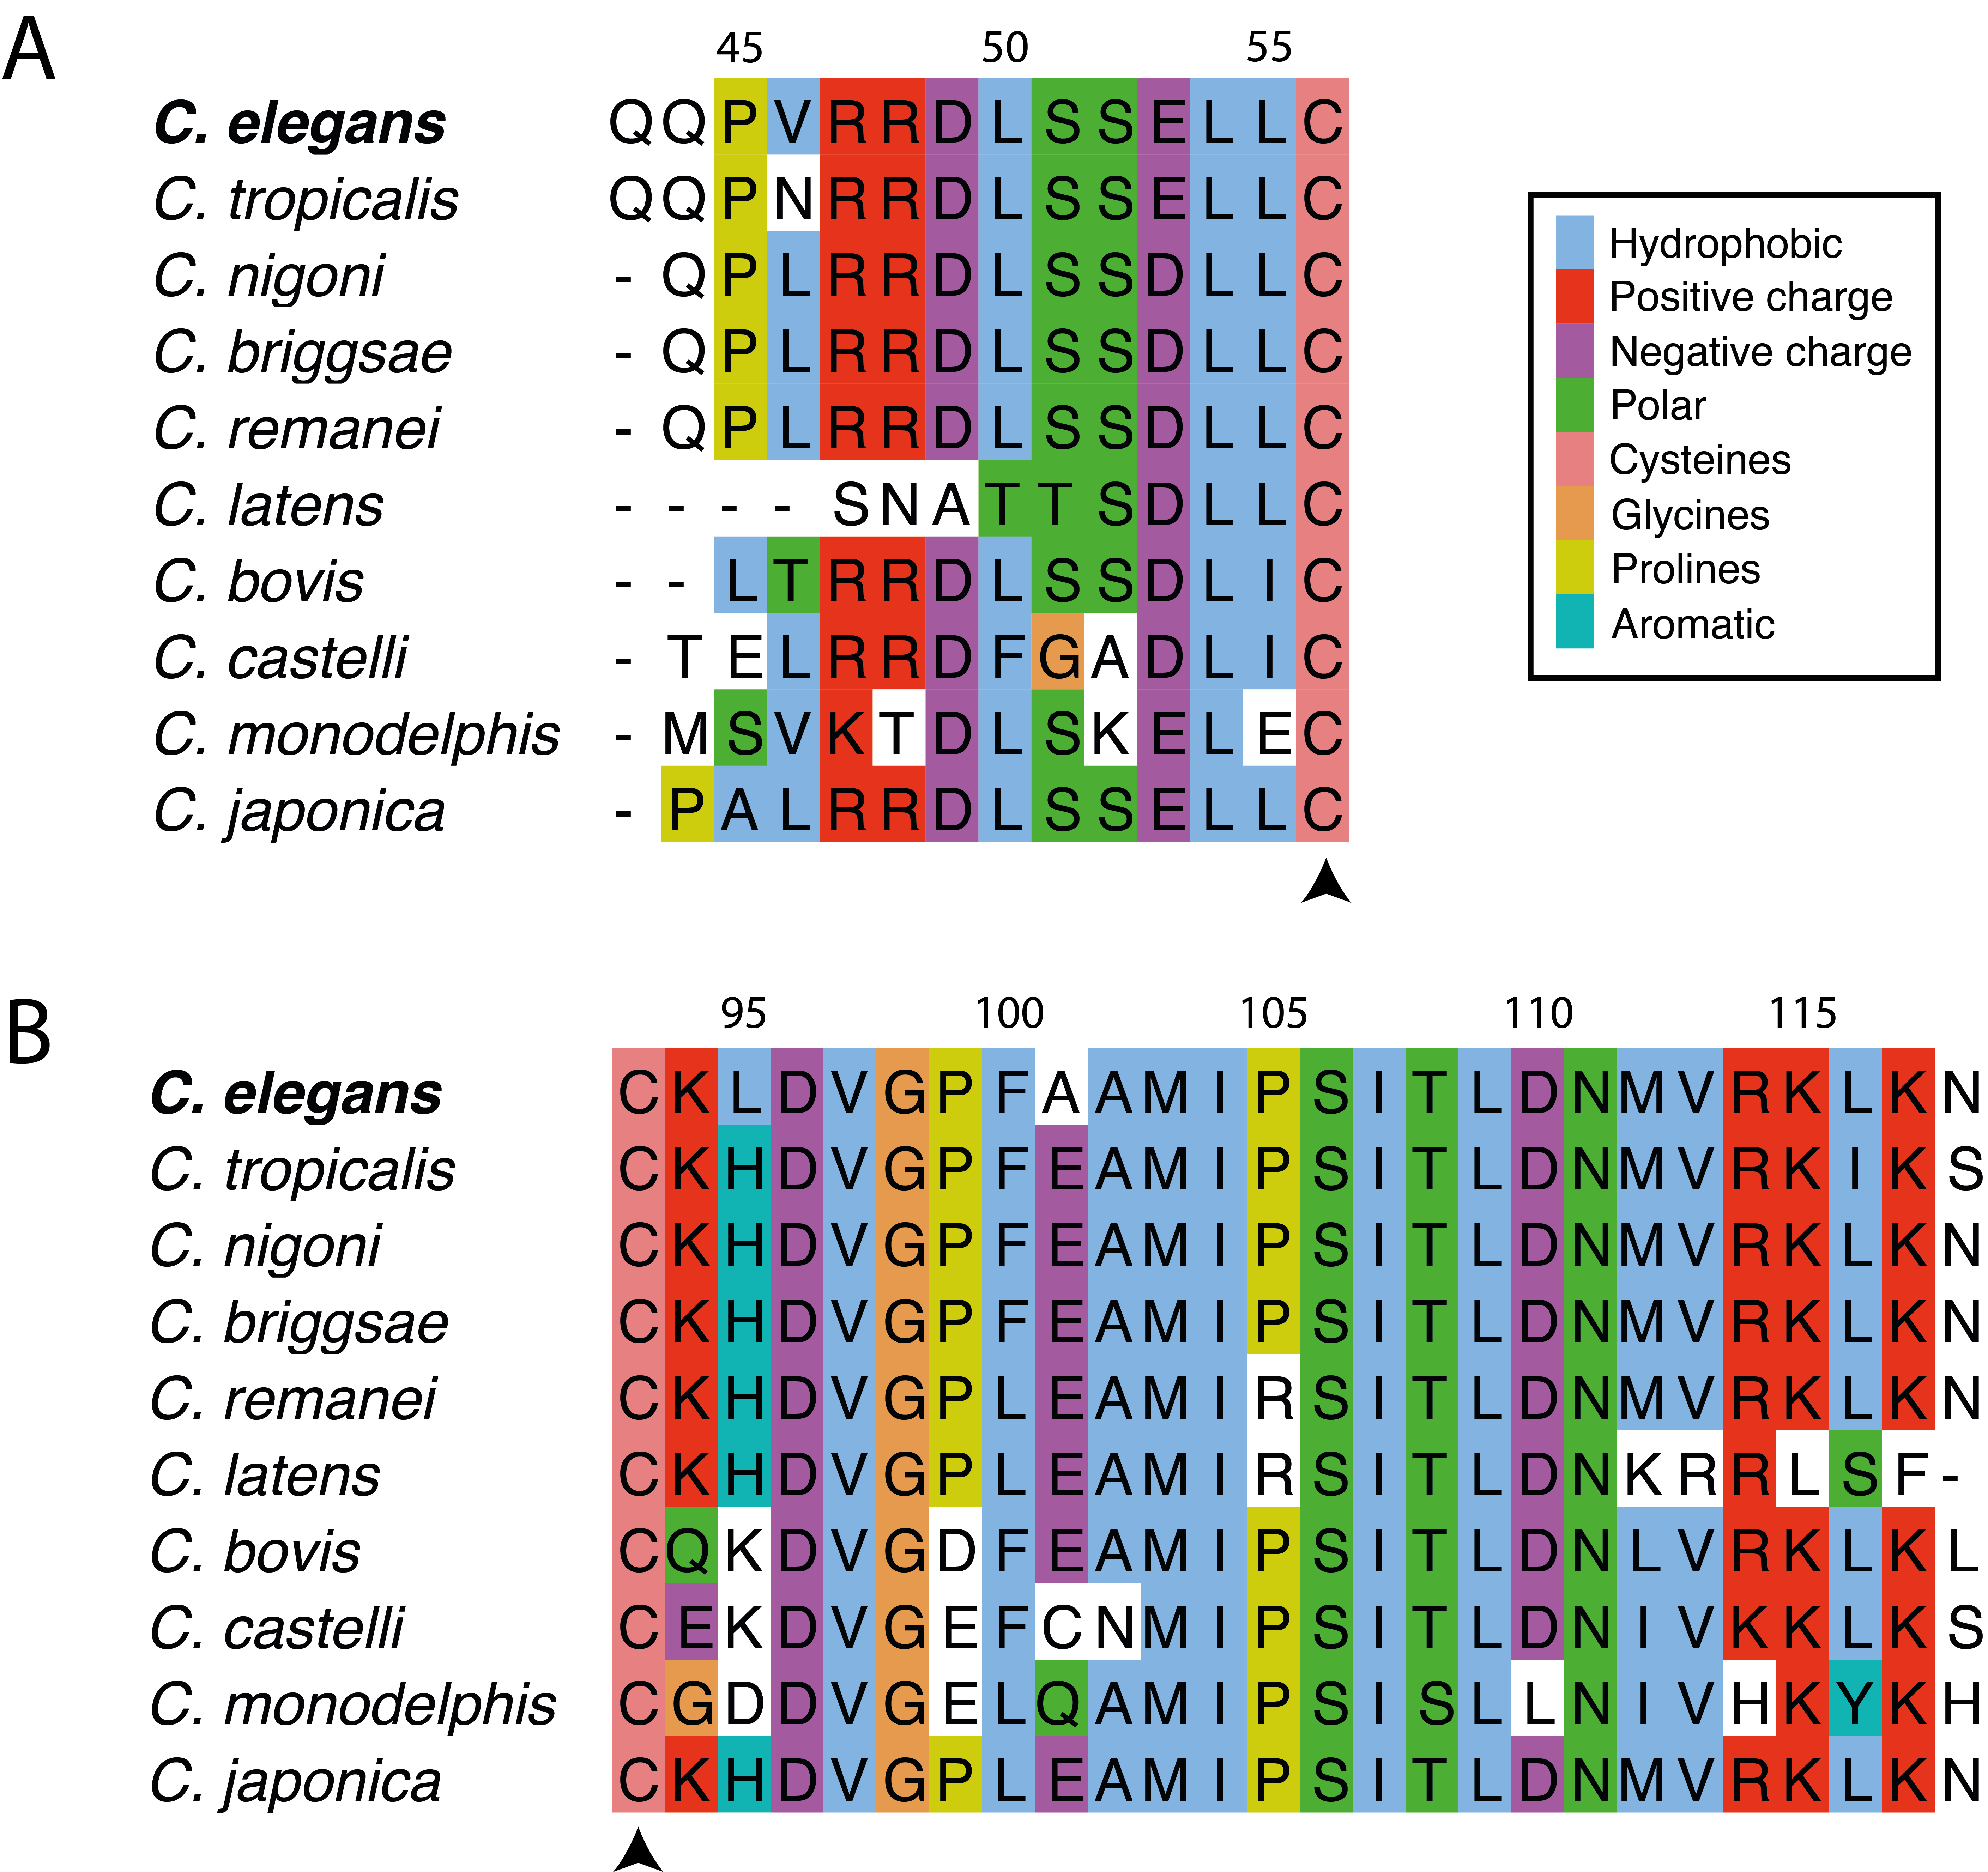
\includegraphics[scale=1]{alignments_par2}
\setlength{\abovecaptionskip}{20pt}
\centering
\mycaption{Title}{Caption}
\label{fig:alignments_par2}
\end{figure}

\clearpage
\subsubsection{RING domain structure prediction}

A number of different methods for predicting the structure. SWISS model tool allows homology modelling, whereby the sequence of interest is mapped to a chosen structure of a protein with high sequence homology. <caveats>. Recently <new methods e.g. alphafold>. \citep{Jumper2021} \\

The predicted structure resembles the common structure of RING domain dimers, characterised by folds around zinc-conjugated ions and a four-helix bundle consisting of an N- and C- helix from each of the two monomers (fig xB). Within this bundle, we see a characteristic pattern of inwards facing hydrophobic residues (fig x). Confidence scores, as measured by pLDDT, are high throughout the structured region of the model.\\


\begin{figure}[!h]
\includegraphics[scale=0.9]{ring_alphafold}
\setlength{\abovecaptionskip}{20pt}
\centering
\mycaption{Title}{Caption}
\label{fig:ring_alphafold}
\end{figure}

\begin{figure}[!h]
\includegraphics[scale=0.9]{ring_alphafold_species}
\setlength{\abovecaptionskip}{20pt}
\centering
\mycaption{Title}{Caption}
\label{fig:ring_alphafold_species}
\end{figure}

Note, at the time of writing, whilst alphafold can model quaternary structures of oligomeric proteins, it relies on the user to input the expected oligomeric state (e.g. dimer in this case), and therefore cannot be used as a tool to predict oligomeric state. Therefore, the resulting structures should be interpreted as the best guess given that dimerisation is expected, which is a reasonable assumption given the common dimeric state of RING domains, and homology of PAR-2 to known dimeric RING domains. Outputted models also do not provide the location of <ions>, but are expected to capture their effects on protein folding.


\clearpage
\subsubsection{Characterising RING domain dimerisation in vitro}

% sec mals on wild type RING

In light of in vivo findings using the C56S mutant, we attempted to express and purify a this mutant for SEC MALS. However, we found the protein to be unstable in vitro and were unable to purify significant quantities, which was not completely unexpected given that the mutation is designed to completely unfold the domain.\\

Instead, we decided to attempt more targeted mutation to the dimerisation interface, aiming to disrupt dimerisation without disrupting the tertiary structure of the domain. This approach has previously been used <examples>. We identified L109, predicted to be found in the C-helical region as a likely important site (fig x), and L109R as a likely disruptive mutation. By contrast to C56S, this mutant was easier to express and purify in sufficient quantities to perform SEC MALS. Strikingly, as shown in fig x, this single mutation completely abrogates dimerisation, showing the expected size for a purely monomeric sample.\\

\begin{figure}[!h]
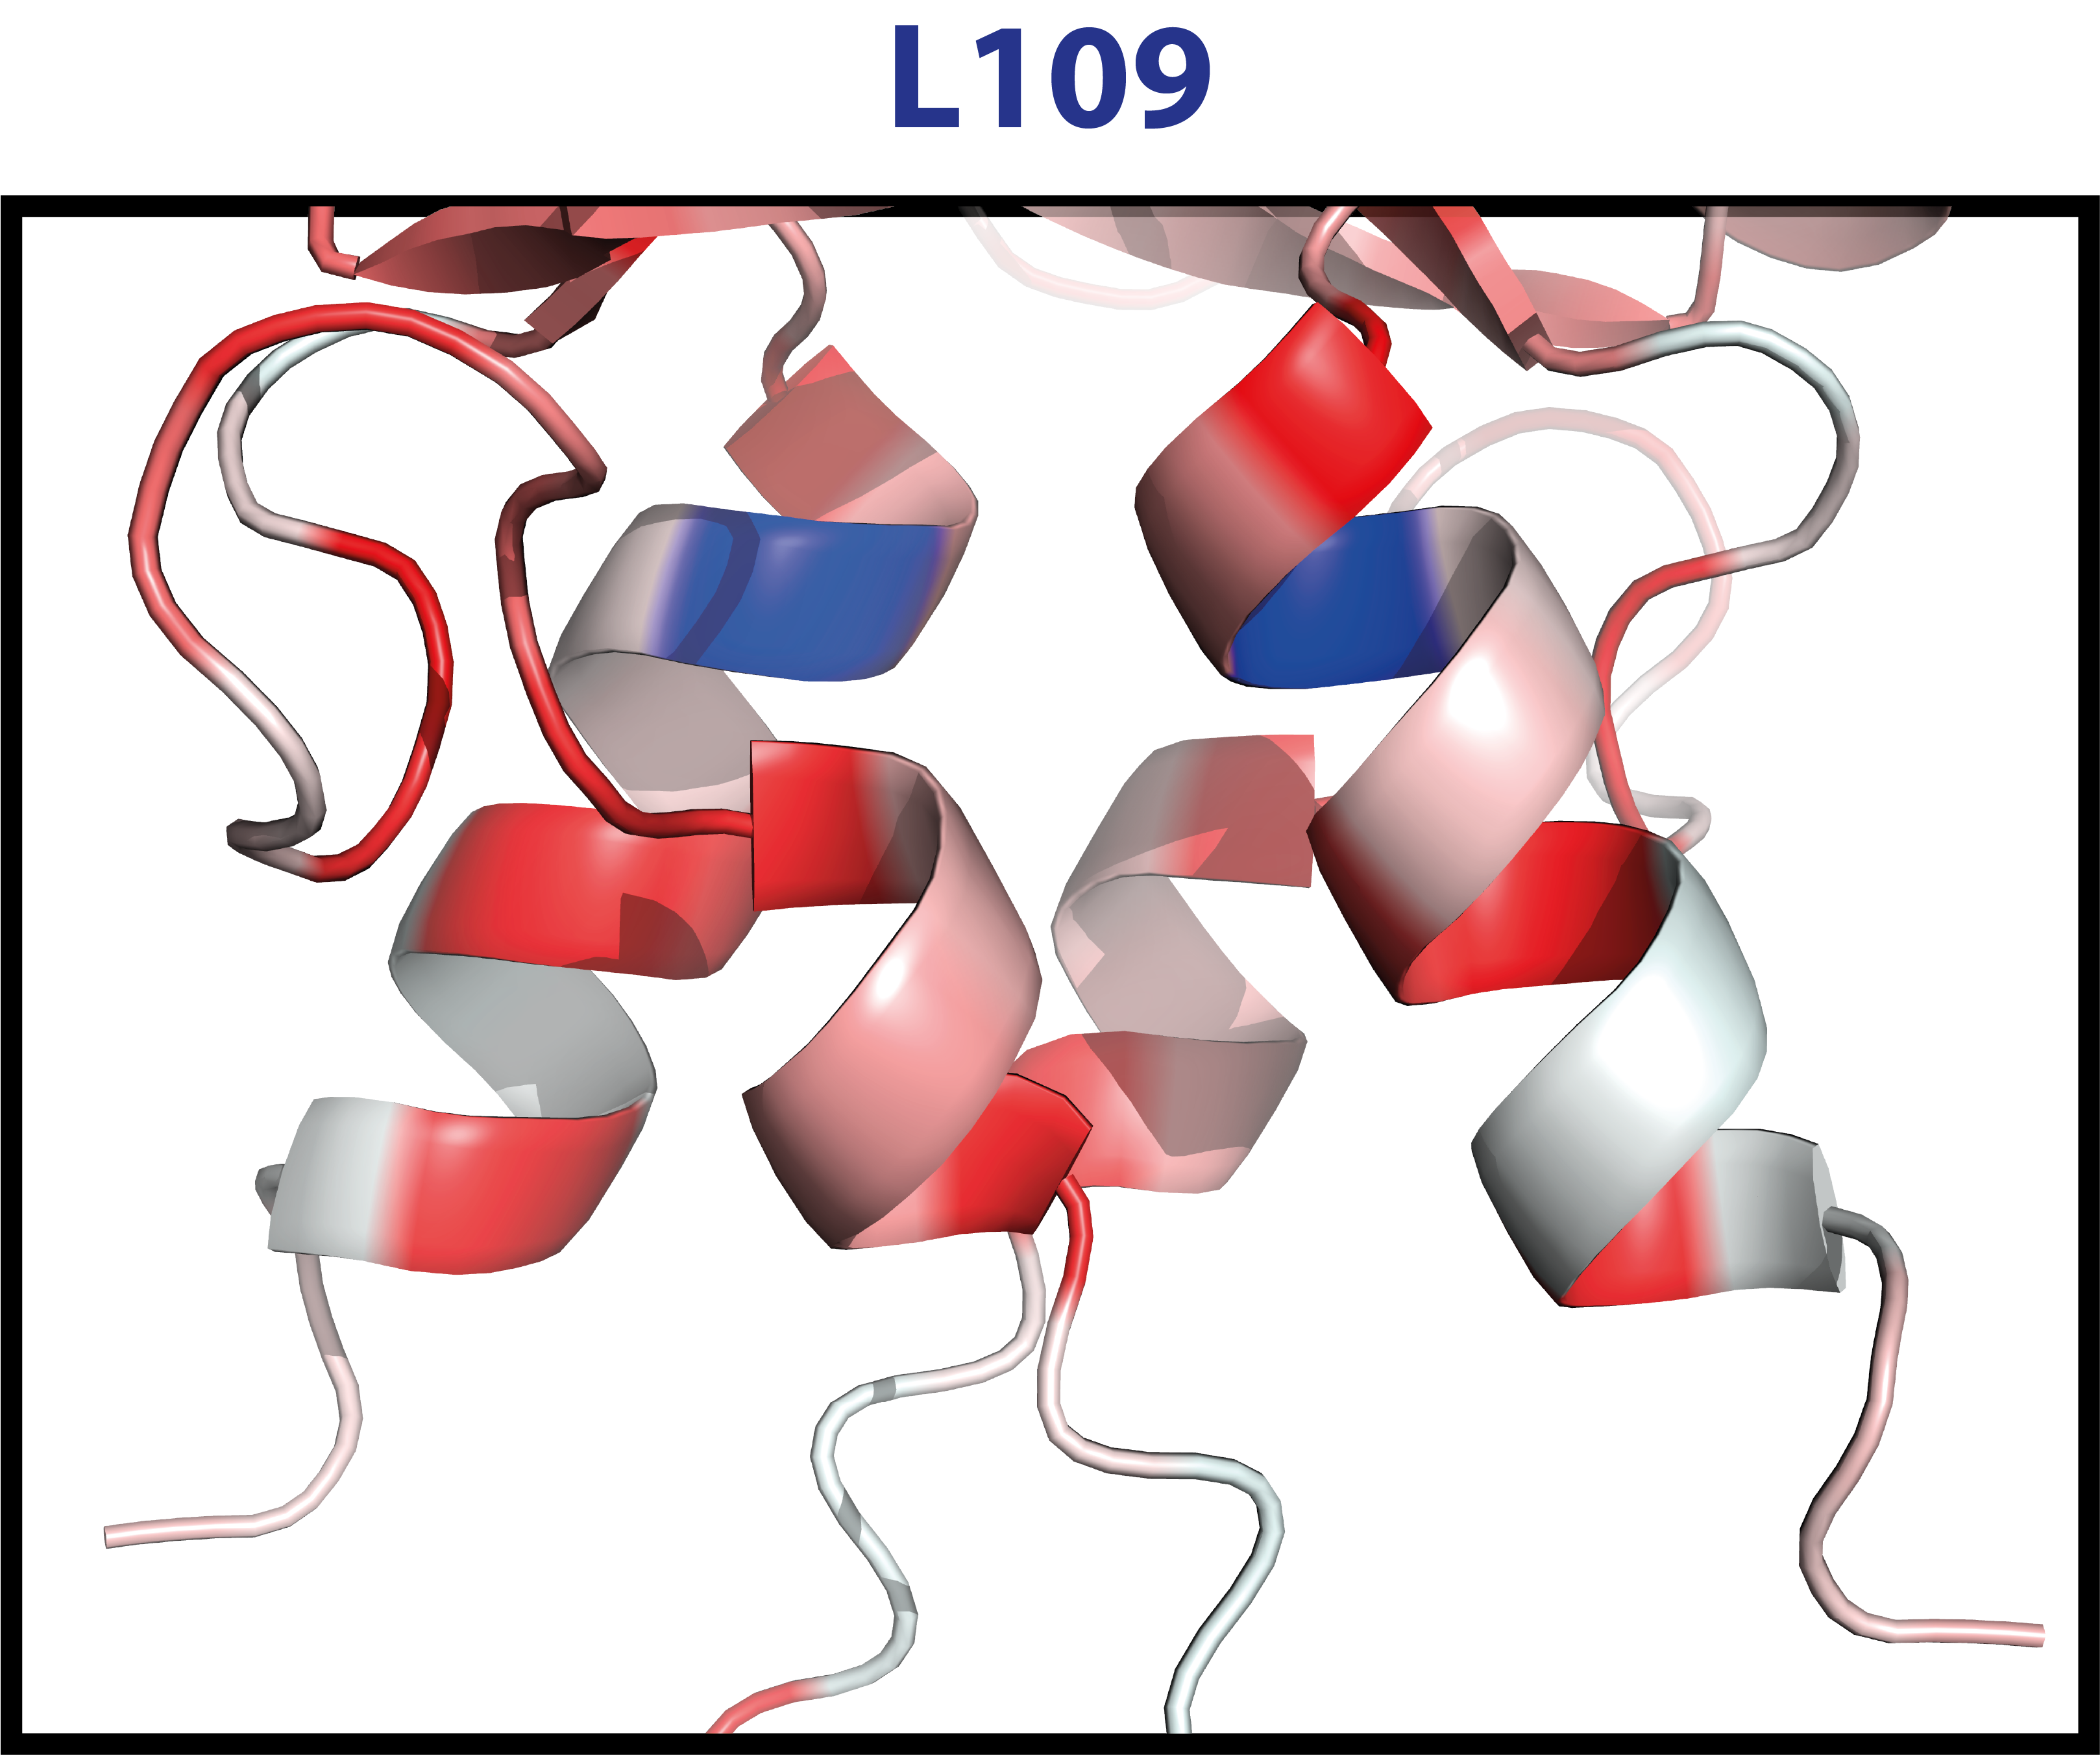
\includegraphics[scale=1]{l109_structure}
\setlength{\abovecaptionskip}{20pt}
\centering
\mycaption{Title}{Caption}
\label{fig:l109_structure}
\end{figure}


\clearpage
\subsubsection{Characterising PAR-2 dimerisation in vivo}

Whilst the above provides convincing evidence that the RING domain of PAR-2 can dimerise in in vitro settings, its ability to drive PAR-2 dimerisation in vivo hasn't been demonstrated. In fact, some evidence exists that would appear to be contradictory to this. Hao showed that an N-terminal fragment (1-177) of PAR-2, which contains the full RING domain but lacks the membrane localisation domain, is entirely cytoplasmic when expressed in vivo. I have also replicated this finding, which is shown in fig x.\\

\begin{figure}[!h]
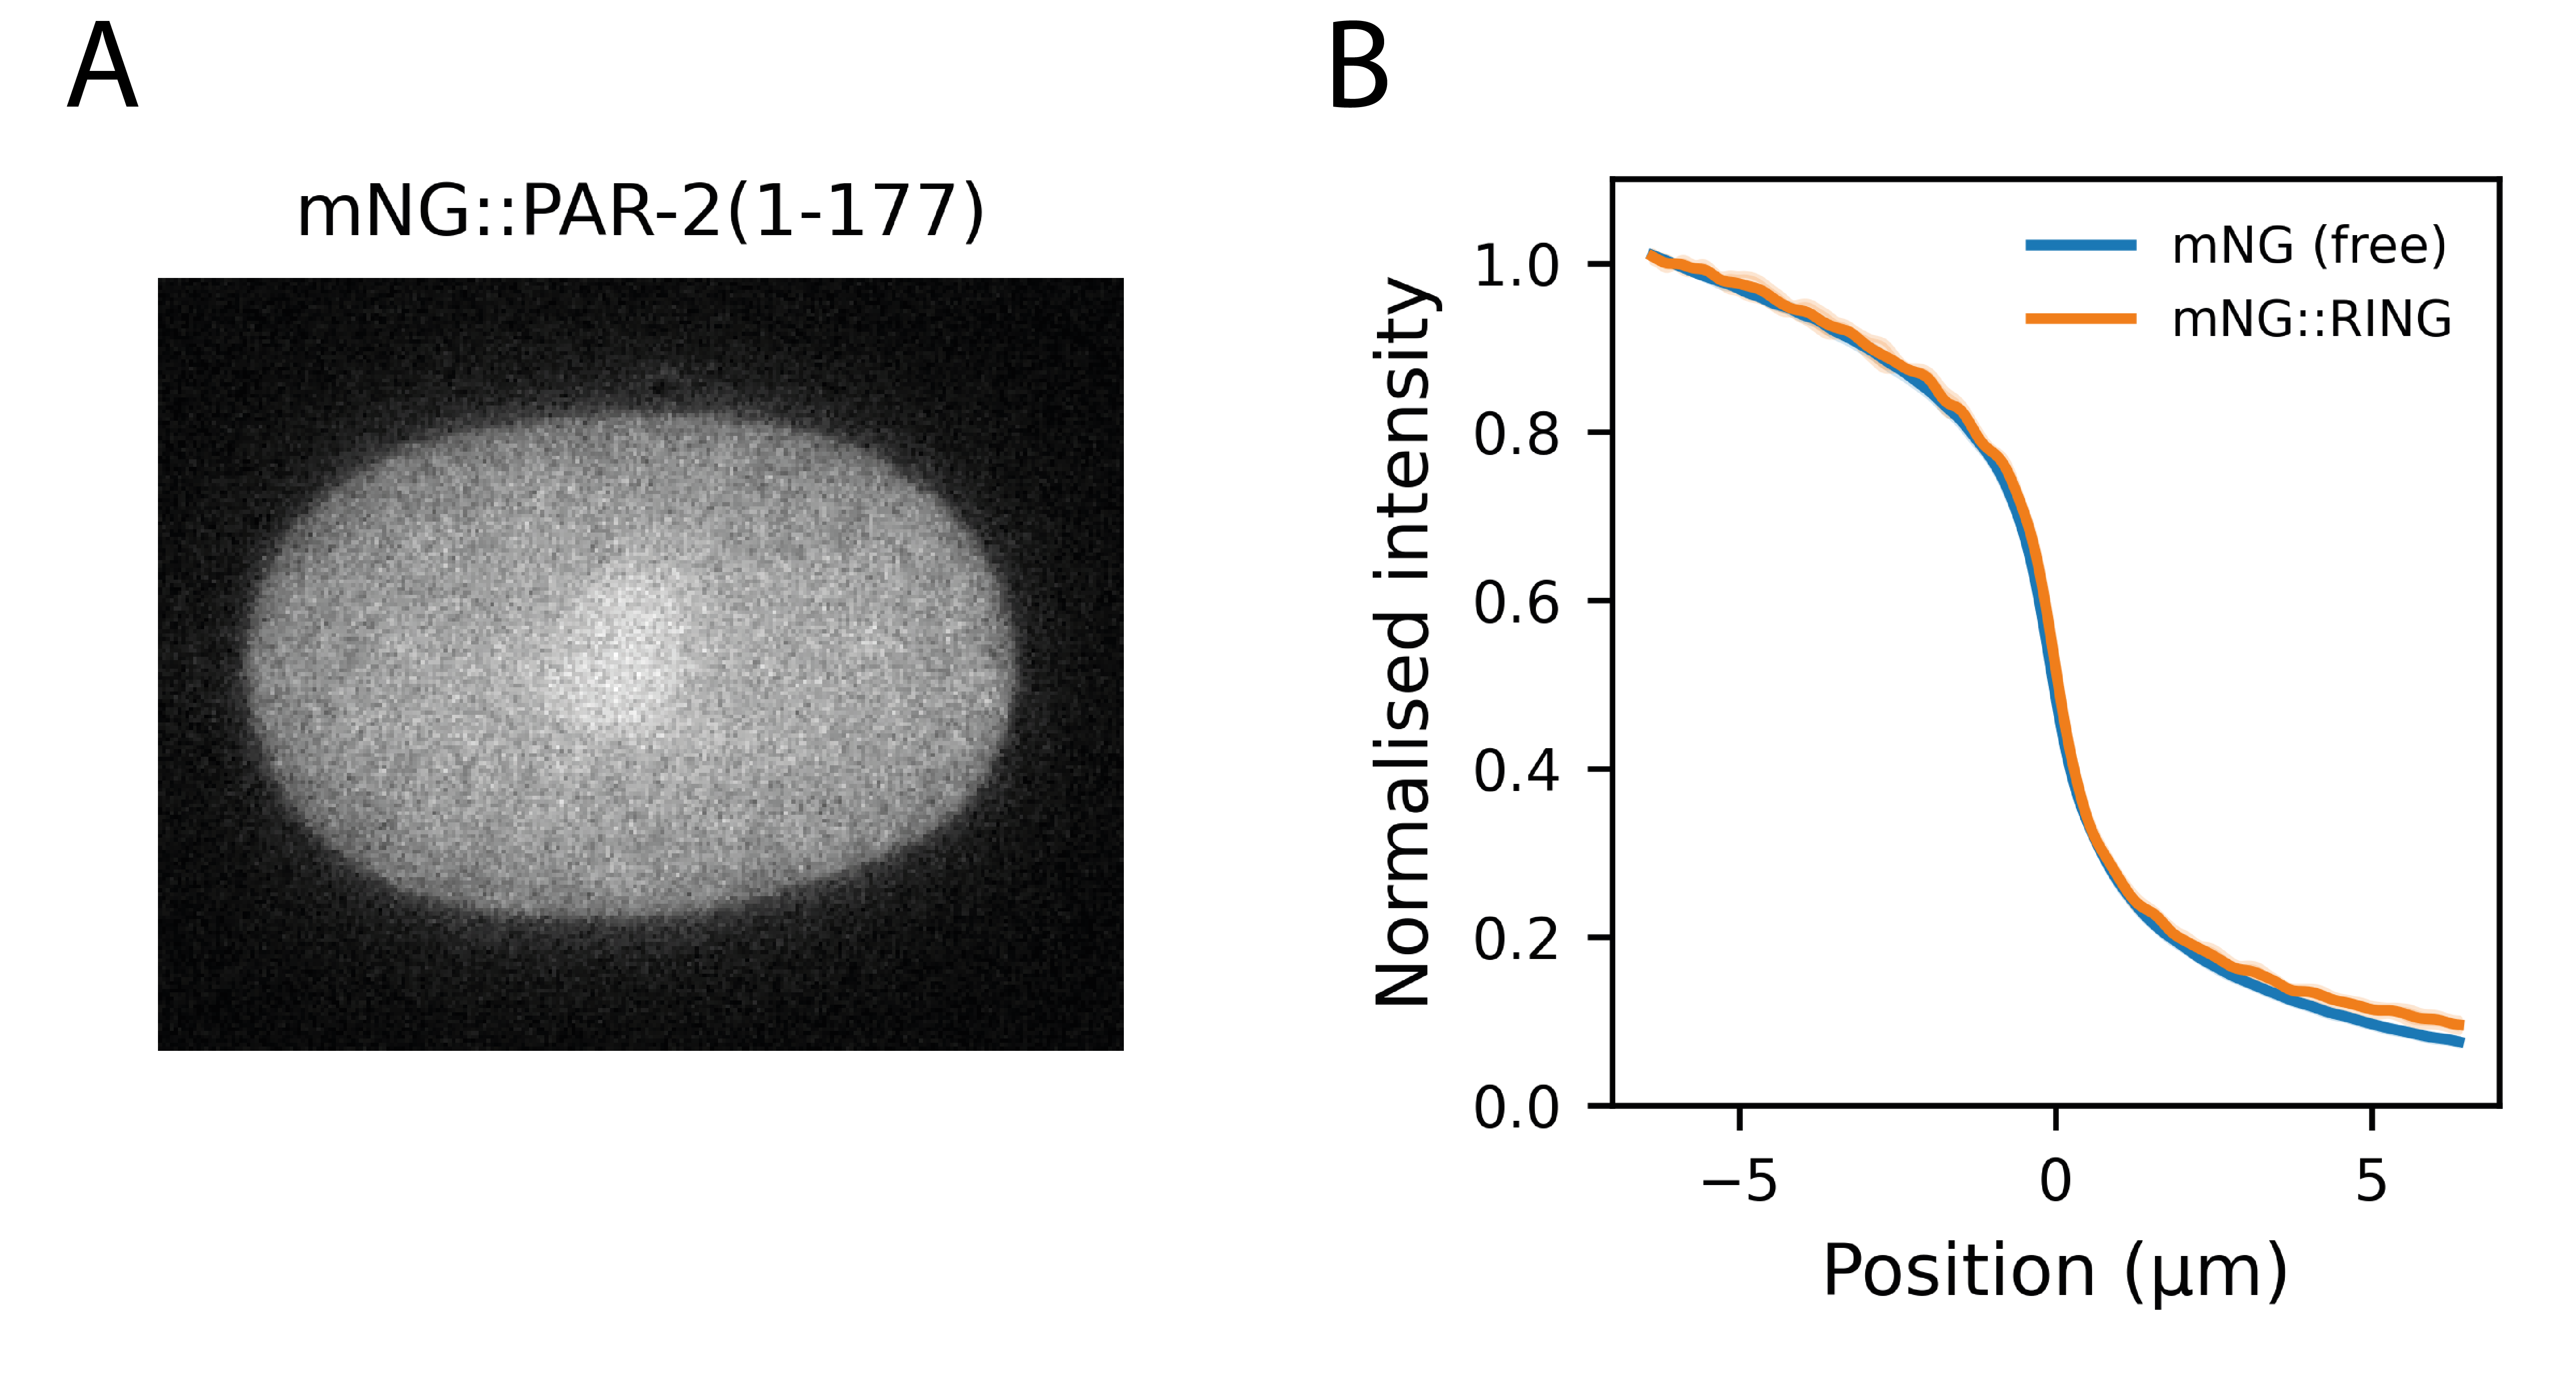
\includegraphics[scale=0.9]{ring_fragment_in_vivo}
\setlength{\abovecaptionskip}{20pt}
\centering
\mycaption{Title}{Caption}
\label{fig:ring_fragment_in_vivo}
\end{figure}

This is surprising, as we would expect that the RING domain fragment should be able to interact with endogenous PAR-2, and thus should, at least partially, colocalise at the posterior membrane. However, given that the fragment contains no intrinsic membrane binding activity, this doesn't exclude the possibility that membrane binding itself is a prerequisite for dimerisation, potentially via concentration-dependent effects.\\

To test whether the RING domain can dimerise when enriched on the membrane, used a PH membrane anchor to tether it to the membrane. Should this construct be capable of dimerisation, we would expect some degree of dimerisation with endogenous PAR-2, end therefore preferential enrichment in the posterior of the cell. Whereas PH alone is uniform on the membrane, tethering the PAR-2 RING domain causes clear enrichment in the posterior, indicating an interaction, presumably a dimerisation reaction, with endogenous PAR-2. A construct with a C56S mutant, by contrast, shows a small degree of polarity, but this is greatly reduced compared to wild type.\\

\begin{figure}[!h]
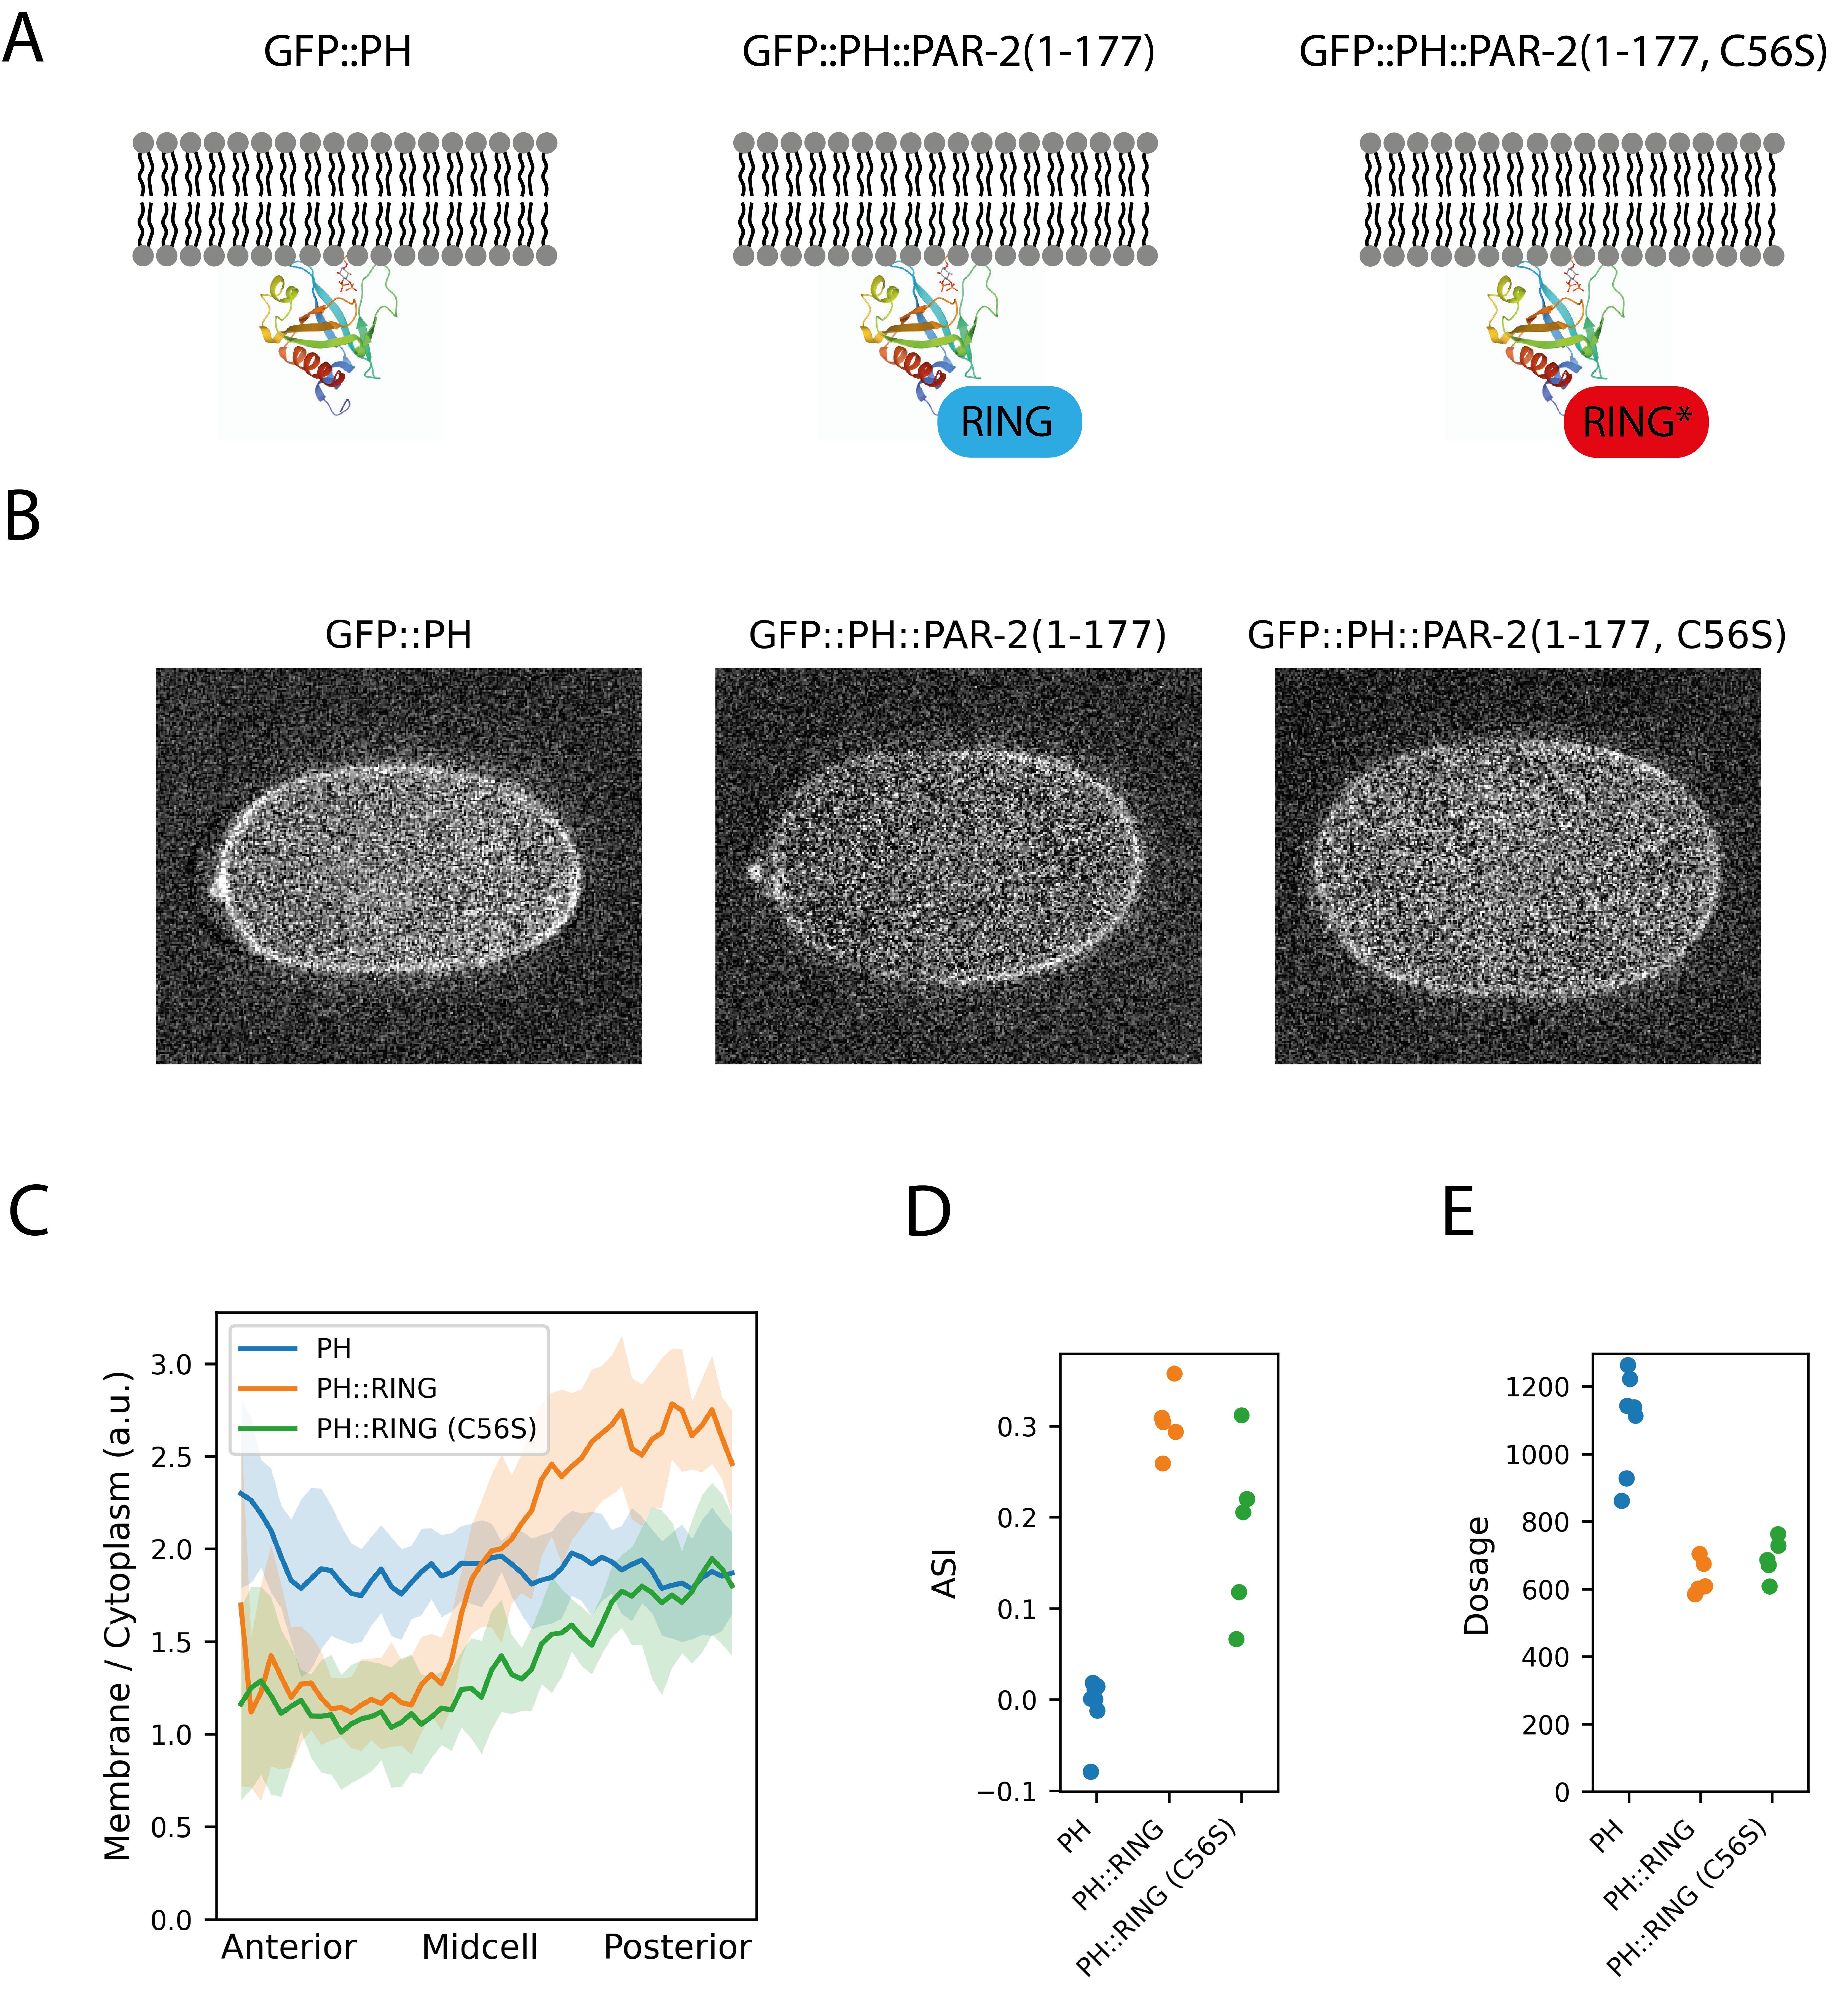
\includegraphics[scale=1]{ph_ring}
\setlength{\abovecaptionskip}{20pt}
\centering
\mycaption{Title}{Caption}
\label{fig:ph_ring}
\end{figure}

The above results suggest that the construct is polarising by responding to polarised endogenous PAR-2. Therefore, it is expected that disrupting polarity of endogenous PAR-2 might disrupt this. To test this, I aimed to disrupt endogenous polarity using RNAi. In conditions of par-2 RNAi, endogenous PAR-2 is expected to be entirely absent from the cell. Under these conditions, as shown in figure x, the construct loses enrichment in the posterior, and overall polarity is low. Similarly, in conditions of par-6 RNAi, where endogenous PAR-2 is expected to be uniform on the cortex, albeit less weakly concentrated, the construct also loses the ability to enrich in the posterior. Whilst we might expect overall affinity to be higher in the par-6 RNAi condition, as there is some level of endogenous PAR-2 on the cortex, this doesn’t appear to be the case. This may imply a concentration dependent effect, whereby the construct is only able to respond to endogenous PAR-2 that’s highly concentrated, or could be a product of inaccurate quantification at very low signal levels.\\

\begin{figure}[!h]
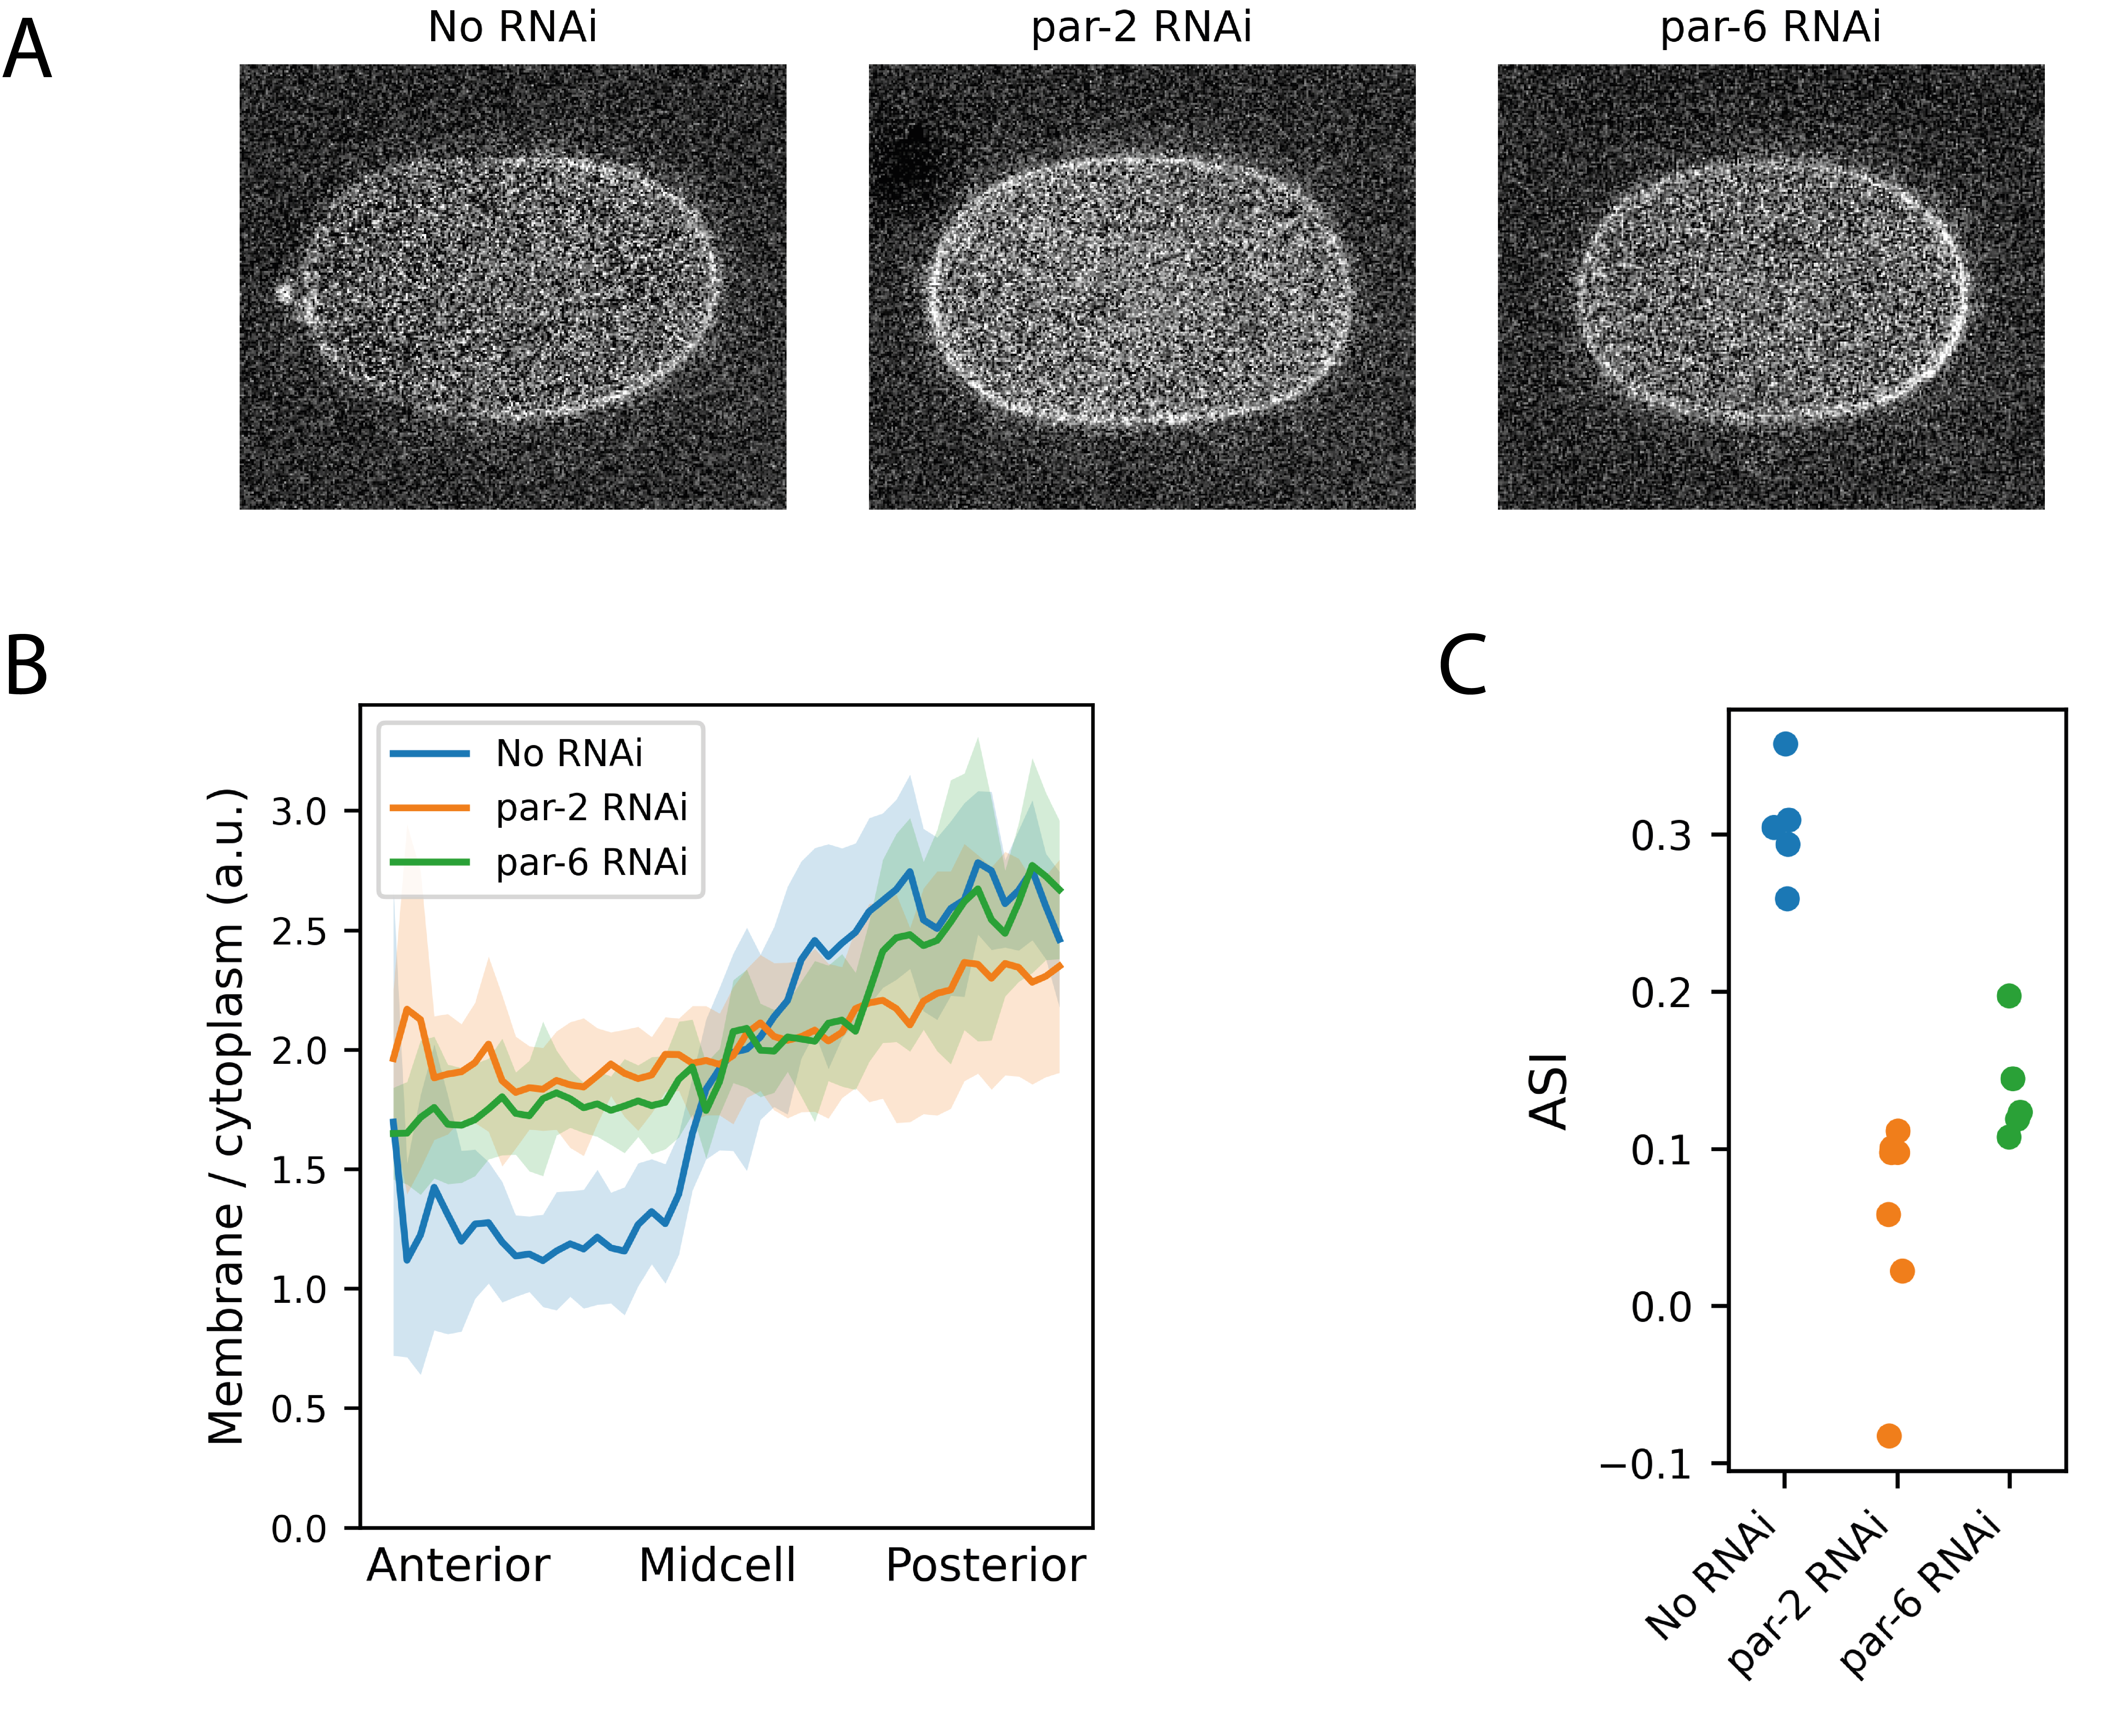
\includegraphics[scale=1]{ph_ring_rnai}
\setlength{\abovecaptionskip}{20pt}
\centering
\mycaption{Title}{Caption}
\label{fig:ph_ring_rnai}
\end{figure}

% more discussion here

The above data implies to a model where PAR-2 is not constitutively dimeric, but can dimerise upon recruitment to the membrane, likely due to concentration-dependent effects. In line with this, we expect that the cytoplasmic pool should be largely, or entirely monomeric. To confirm this I devised in vivo pull-down assay based on dual labelling of PAR-2 with two different fluorophores, fig x. Expressing PAR-2 with a mix of green and red fluorophores means that, were PAR-2 to form constitutive dimers, a mixed population of green/green, green/red and red/red dimers would be expected to be present within the cytoplasm. Thus, forced relocalisation of one of these pools to an exogenous location in the cell should result in a detectable signal of the other fluorophore. A similar assay was used previously by \textcite{Reich2019}, who demonstrated a stable interaction between PAR-6 and PKC-3, through forced localisation of GFP::PKC-3 to the plasma membrane with a membrane-tethered GFP nanobody. (In this case the plasma membrane was a suitable target because, under the conditions of the assay, PAR-6/PKC-3 do not normally bind to the PM). Here I propose a similar approach, relying instead on recruitment to mitochondrial membranes within the cell. Mitochondrial membranes are dense within the cell, and can be probed easily with a localisation signal from the TOMM-20 protein (ref).\\

\begin{figure}[!h]
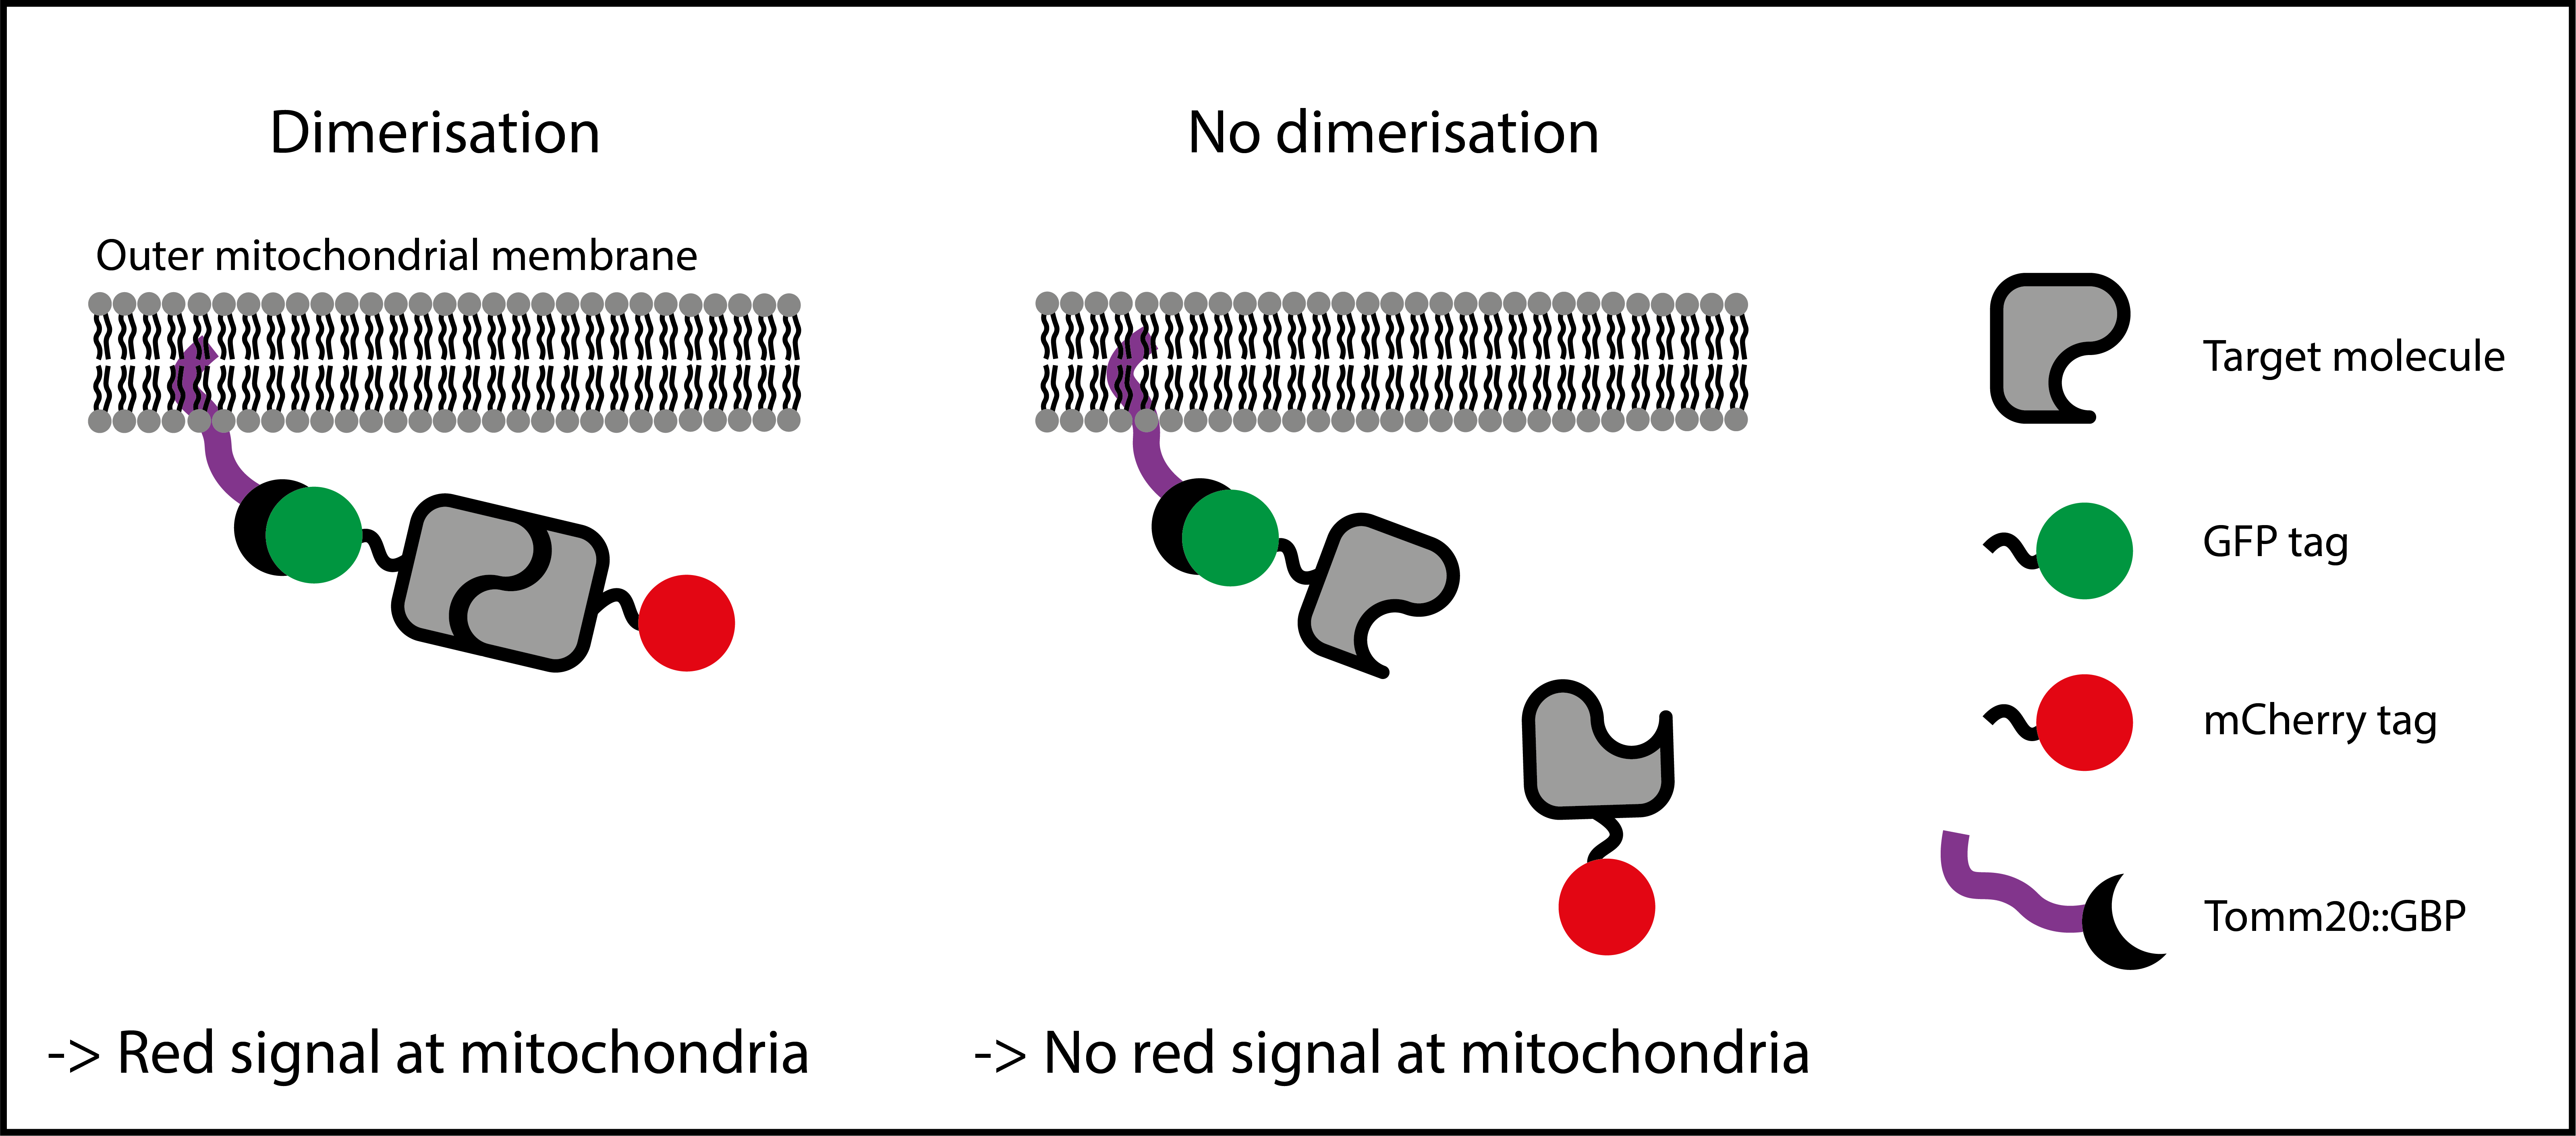
\includegraphics[scale=0.95]{tomm20_schematic}
\setlength{\abovecaptionskip}{20pt}
\centering
\mycaption{Title}{Caption}
\label{fig:tomm20_schematic}
\end{figure}

To first test the potential utility of this method, I built a TOMM-20::GBP probe tagged with mKate, and introduced this into the worm by CRISPR. Crossing this line to GFP::PAR-2, and imaging the F1s (heterozygous for both GFP::PAR-2 and the probe), shows that the probe is well expressed, displays the expected mitochondrial localisation pattern, and is able to recruit GFP::PAR-2 to the mitochondria.\\

\begin{figure}[!h]
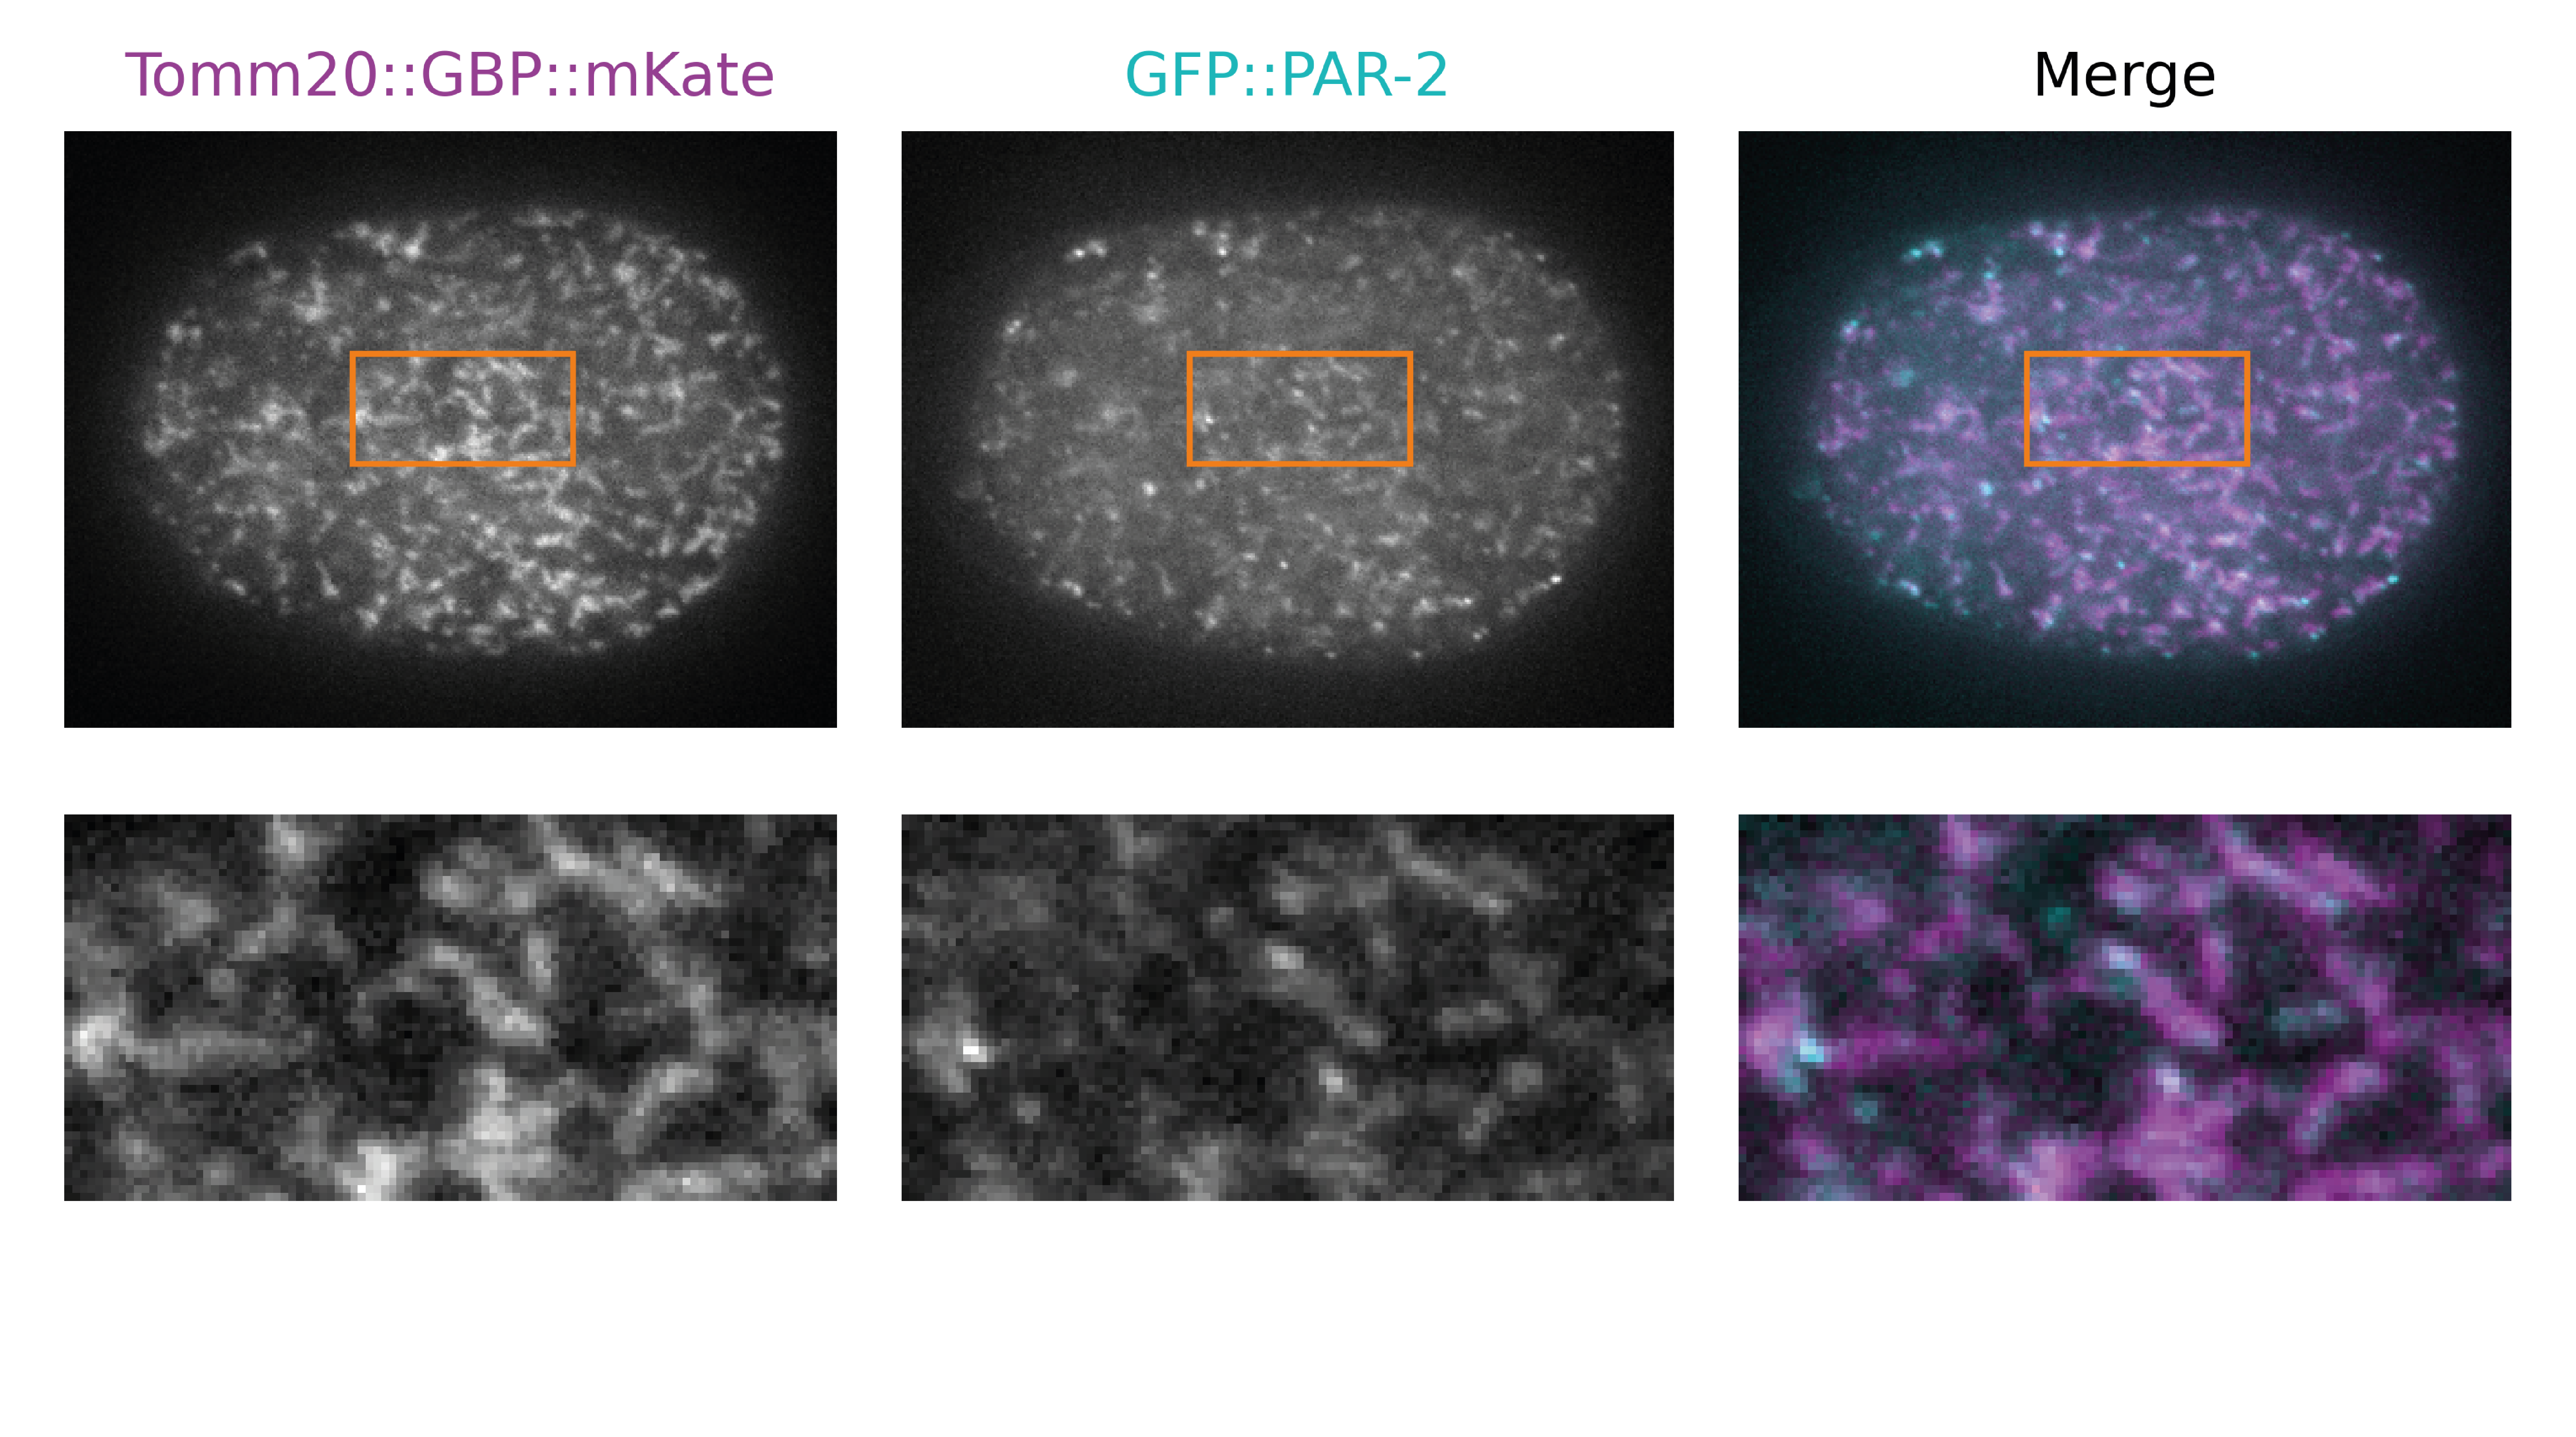
\includegraphics[scale=0.95]{tomm20_merge}
\setlength{\abovecaptionskip}{20pt}
\centering
\mycaption{Title}{Caption}
\label{fig:tomm20_merge}
\end{figure}

To perform the proposed dimerisation assay, I next attempted to build an untagged version of the probe (lacking mKate). Whilst I was successfully able to build and introduce the construct into the genome of the worm, I found that this untagged probe failed to recruit any GFP::PAR-2 to the mitochondria, likely indicating that the probe failed to express. This suggests that the mKate tag may be stabilising expression of the full construct, possibly due to the presence of introns within the mKate sequence. As an alternative method to free up the red channel, I introduced a point mutation into mKate by CRISPR designed to disrupt the chromophore region (ref). This construct, by contrast, was well expressed and, like the tagged parent construct, able to pull GFP::PAR-2 to the mitochondria. Next, I crossed this line to a line expressing PAR-2::mCherry at the endogenous locus, homozygosing both constructs. I then crossed this line to a line homozygous for endogenous GFP::PAR-2, giving F1s heterozygous for GFP/mCherry PAR-2, and heterozygous for the probe.  Imaging embryos from these F1s showed that, whereas GFP::PAR-2 is fully pulled to the mitochondria, there is no detectable colocalisation with mCherry::PAR-2.\\

\begin{figure}[!h]
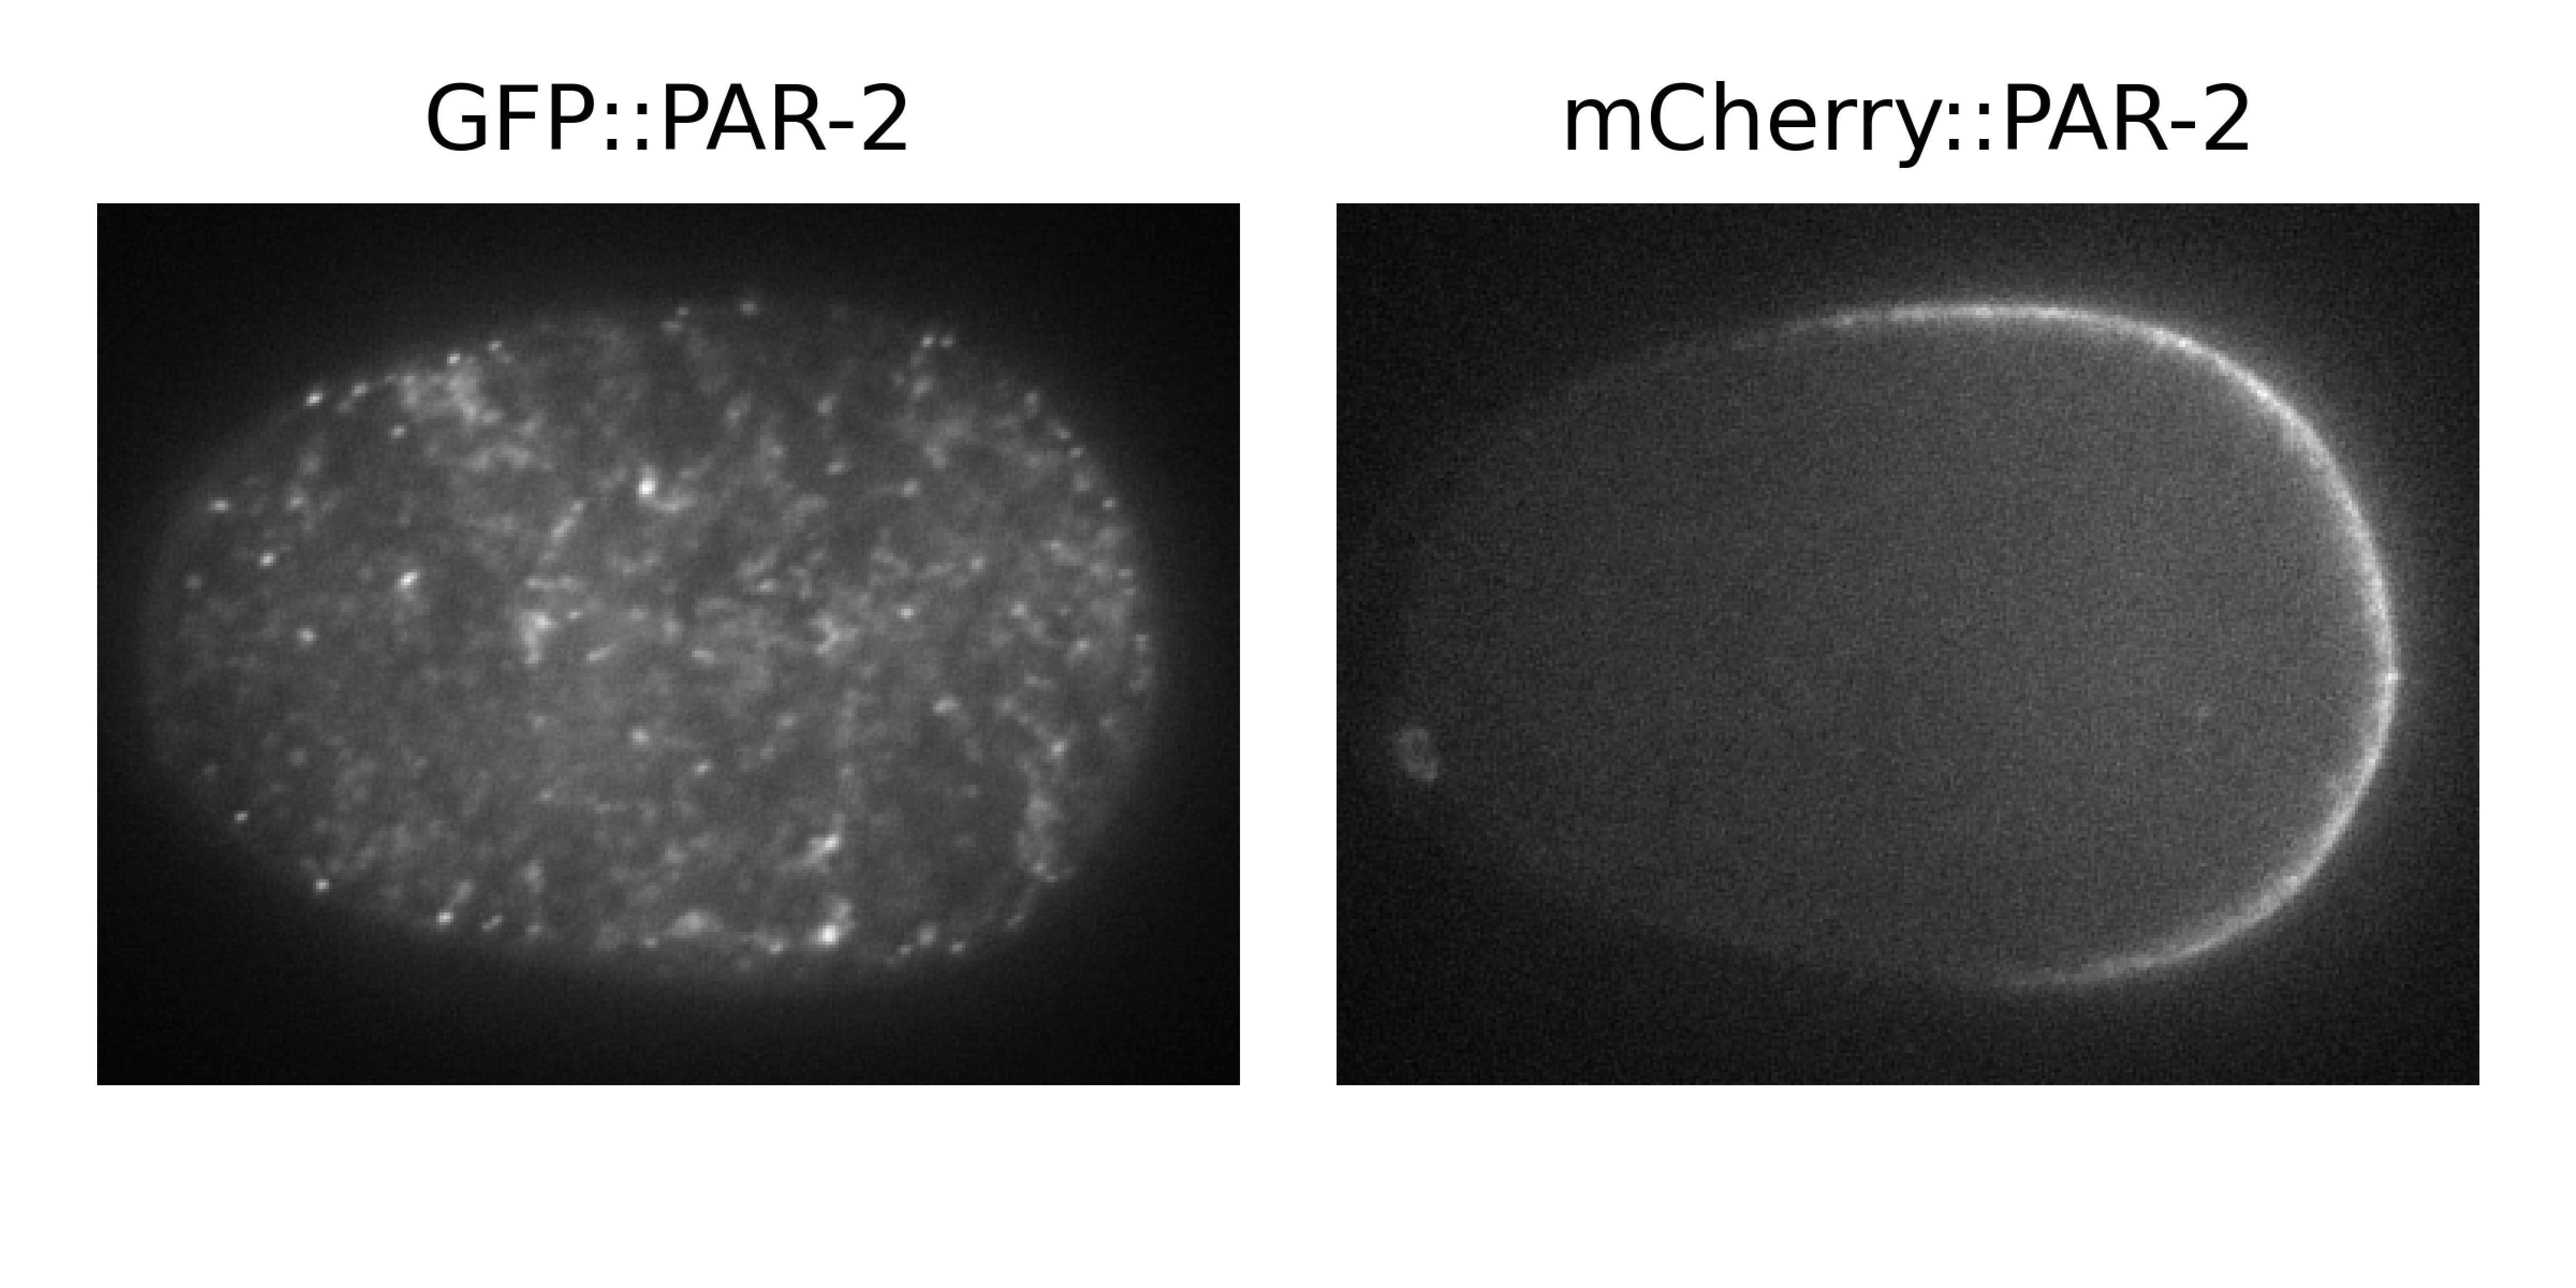
\includegraphics[scale=1]{tomm20_assay}
\setlength{\abovecaptionskip}{20pt}
\centering
\mycaption{Title}{Caption}
\label{fig:tomm20_assay}
\end{figure}

% summary/discussion. Reiterate concentration-dependent dimerisation model.

\clearpage
\subsubsection{Targeted mutation to dimerisation interface regions}

As discussed previously, disrupting the RING domain, by targeted mutation to a zinc-interacting cysteine, has a strong phenotype in vivo, characterised by a string reduction in membrane affinity. My results suggest that this phenotype may be explained by a disruption in dimerisation at the membrane. However, as C56S mutation disrupts the tertiary structure of the whole domain, rather than just the dimerisation interface, it may also have additional effects. To confirm the specific role of dimerisation, I performed targeted mutations to the dimerisation interface region of the RING domain, aiming to disrupt dimerisation in vivo whilst keeping the tertiary structure of the domain intact. In addition to L109R, I performed an additional L>R mutation to L50, which is found in the N-helix. I introduced mutations at the endogenous site by CRISPR in an mNeonGreen::PAR-2 line. \\

\begin{figure}[!h]
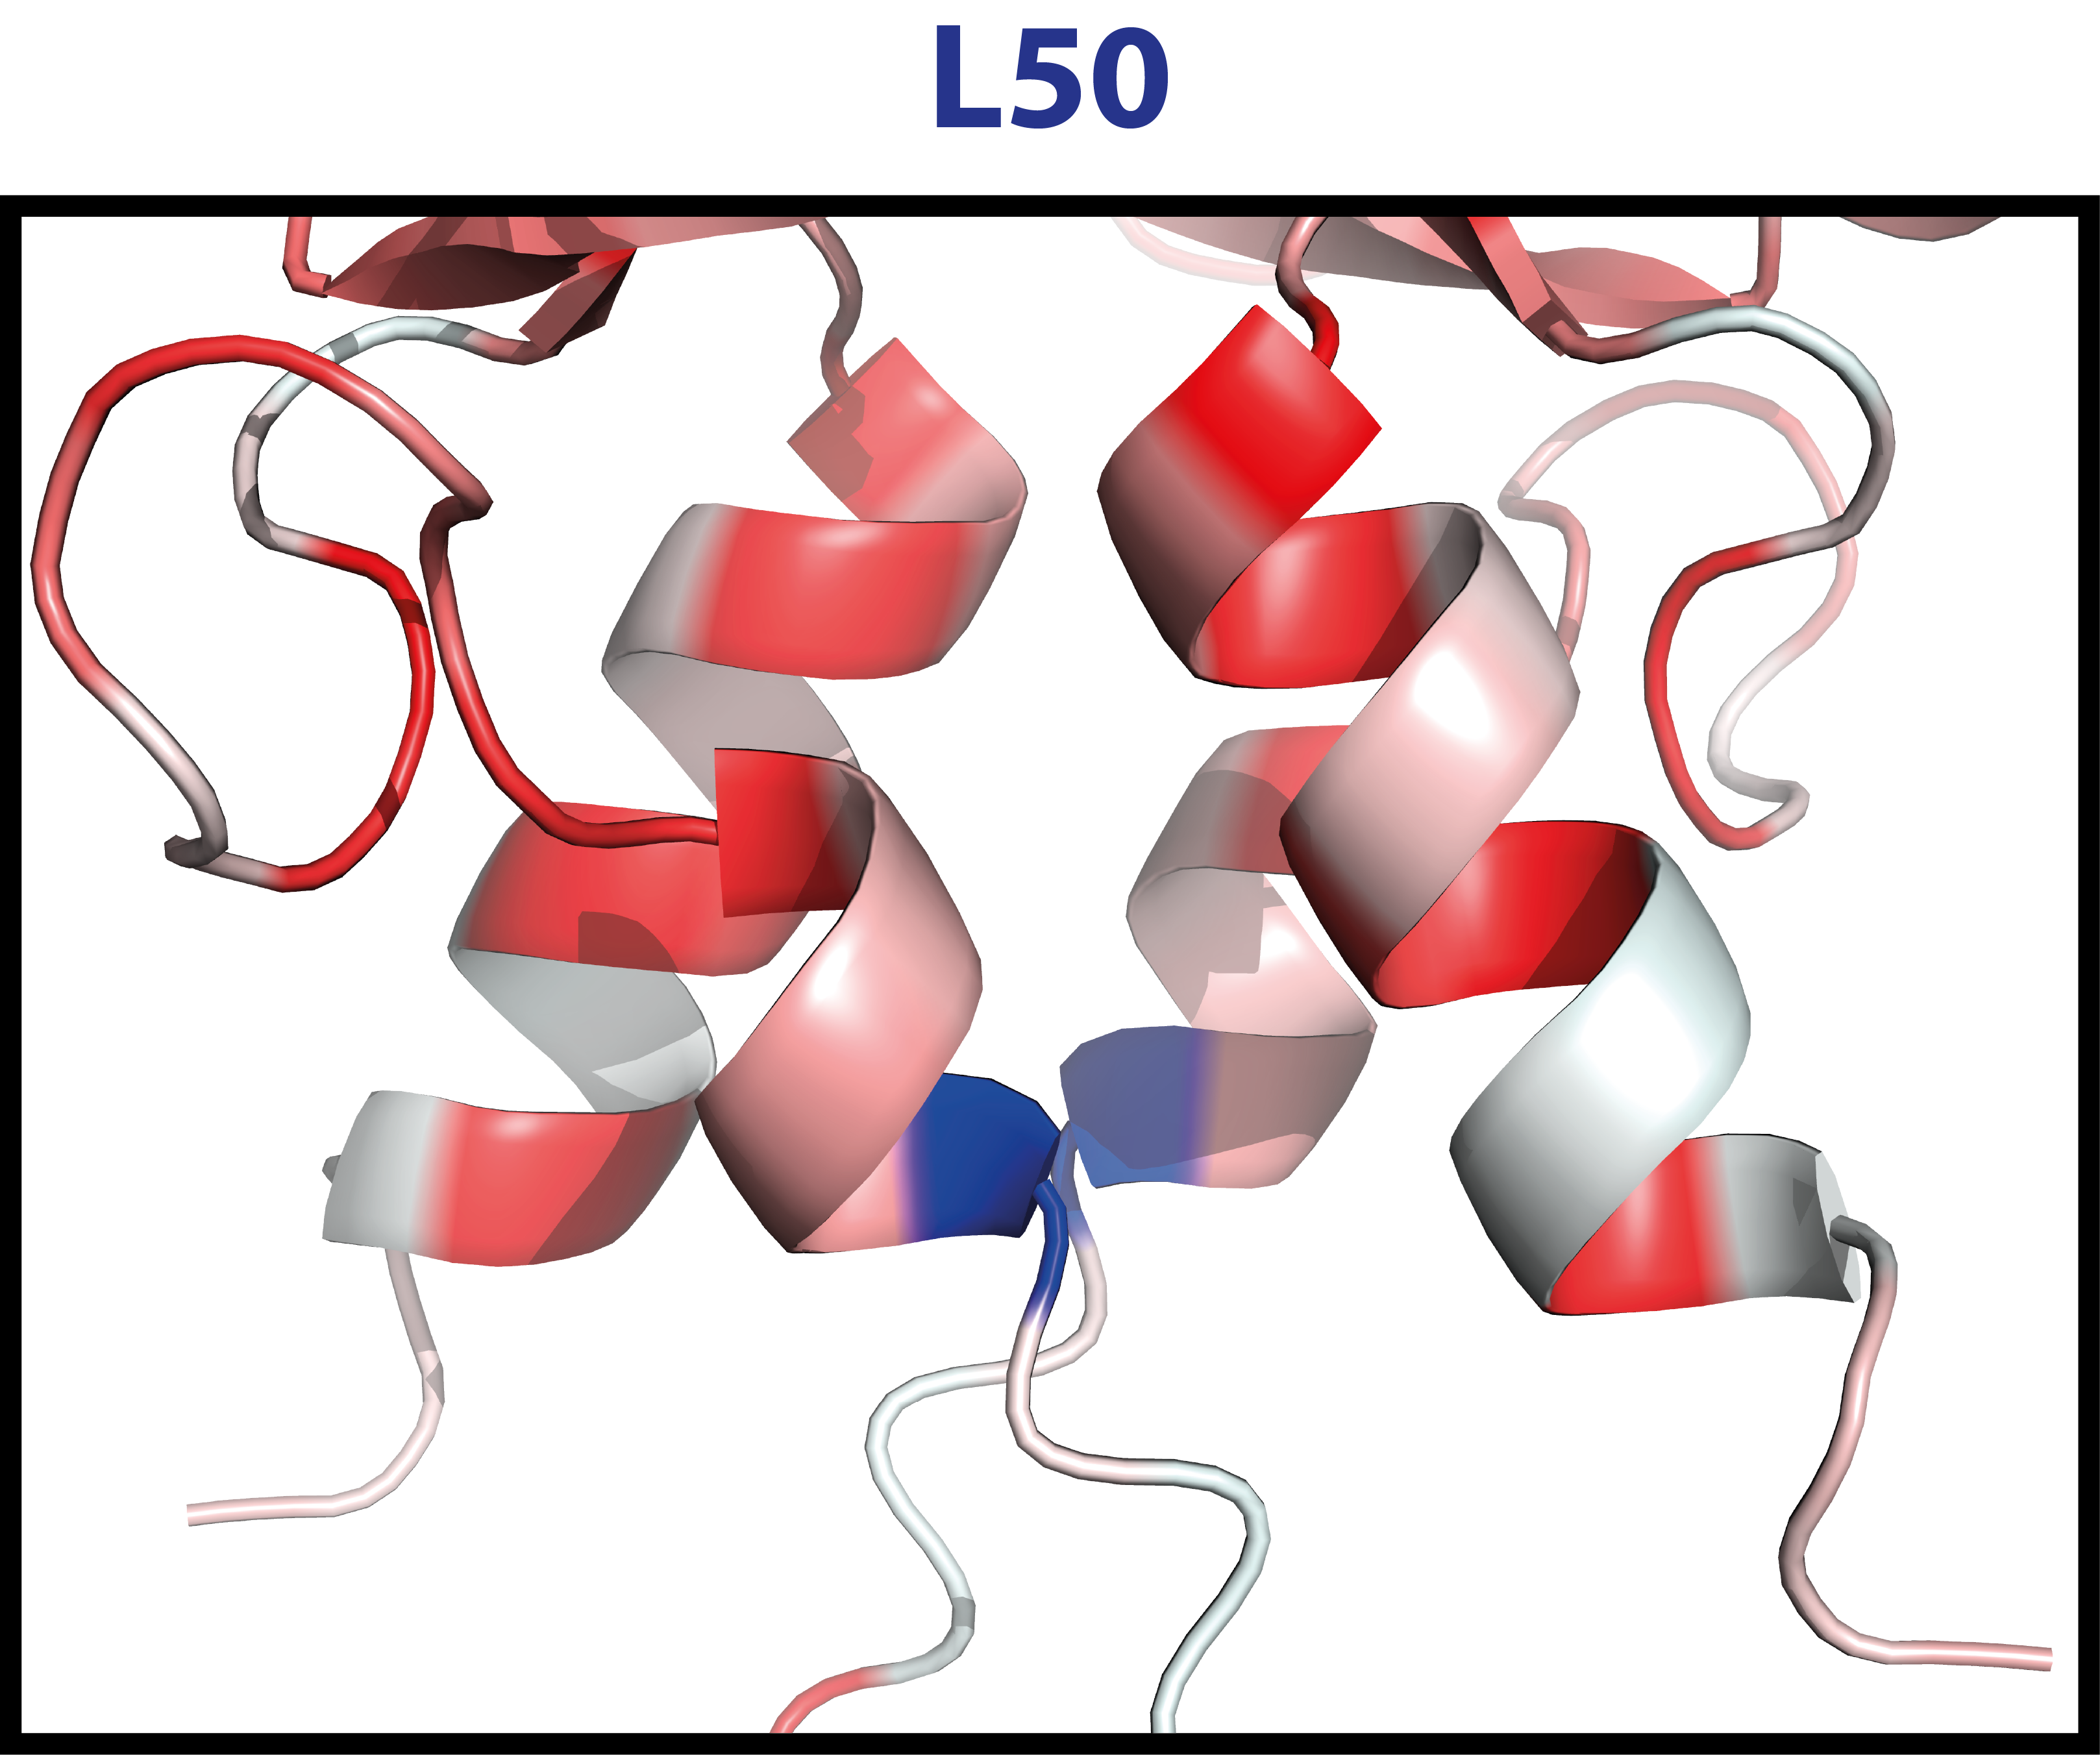
\includegraphics[scale=0.9]{l50_structure}
\setlength{\abovecaptionskip}{20pt}
\centering
\mycaption{Title}{Caption}
\label{fig:l50_structure}
\end{figure}


\begin{figure}[!h]
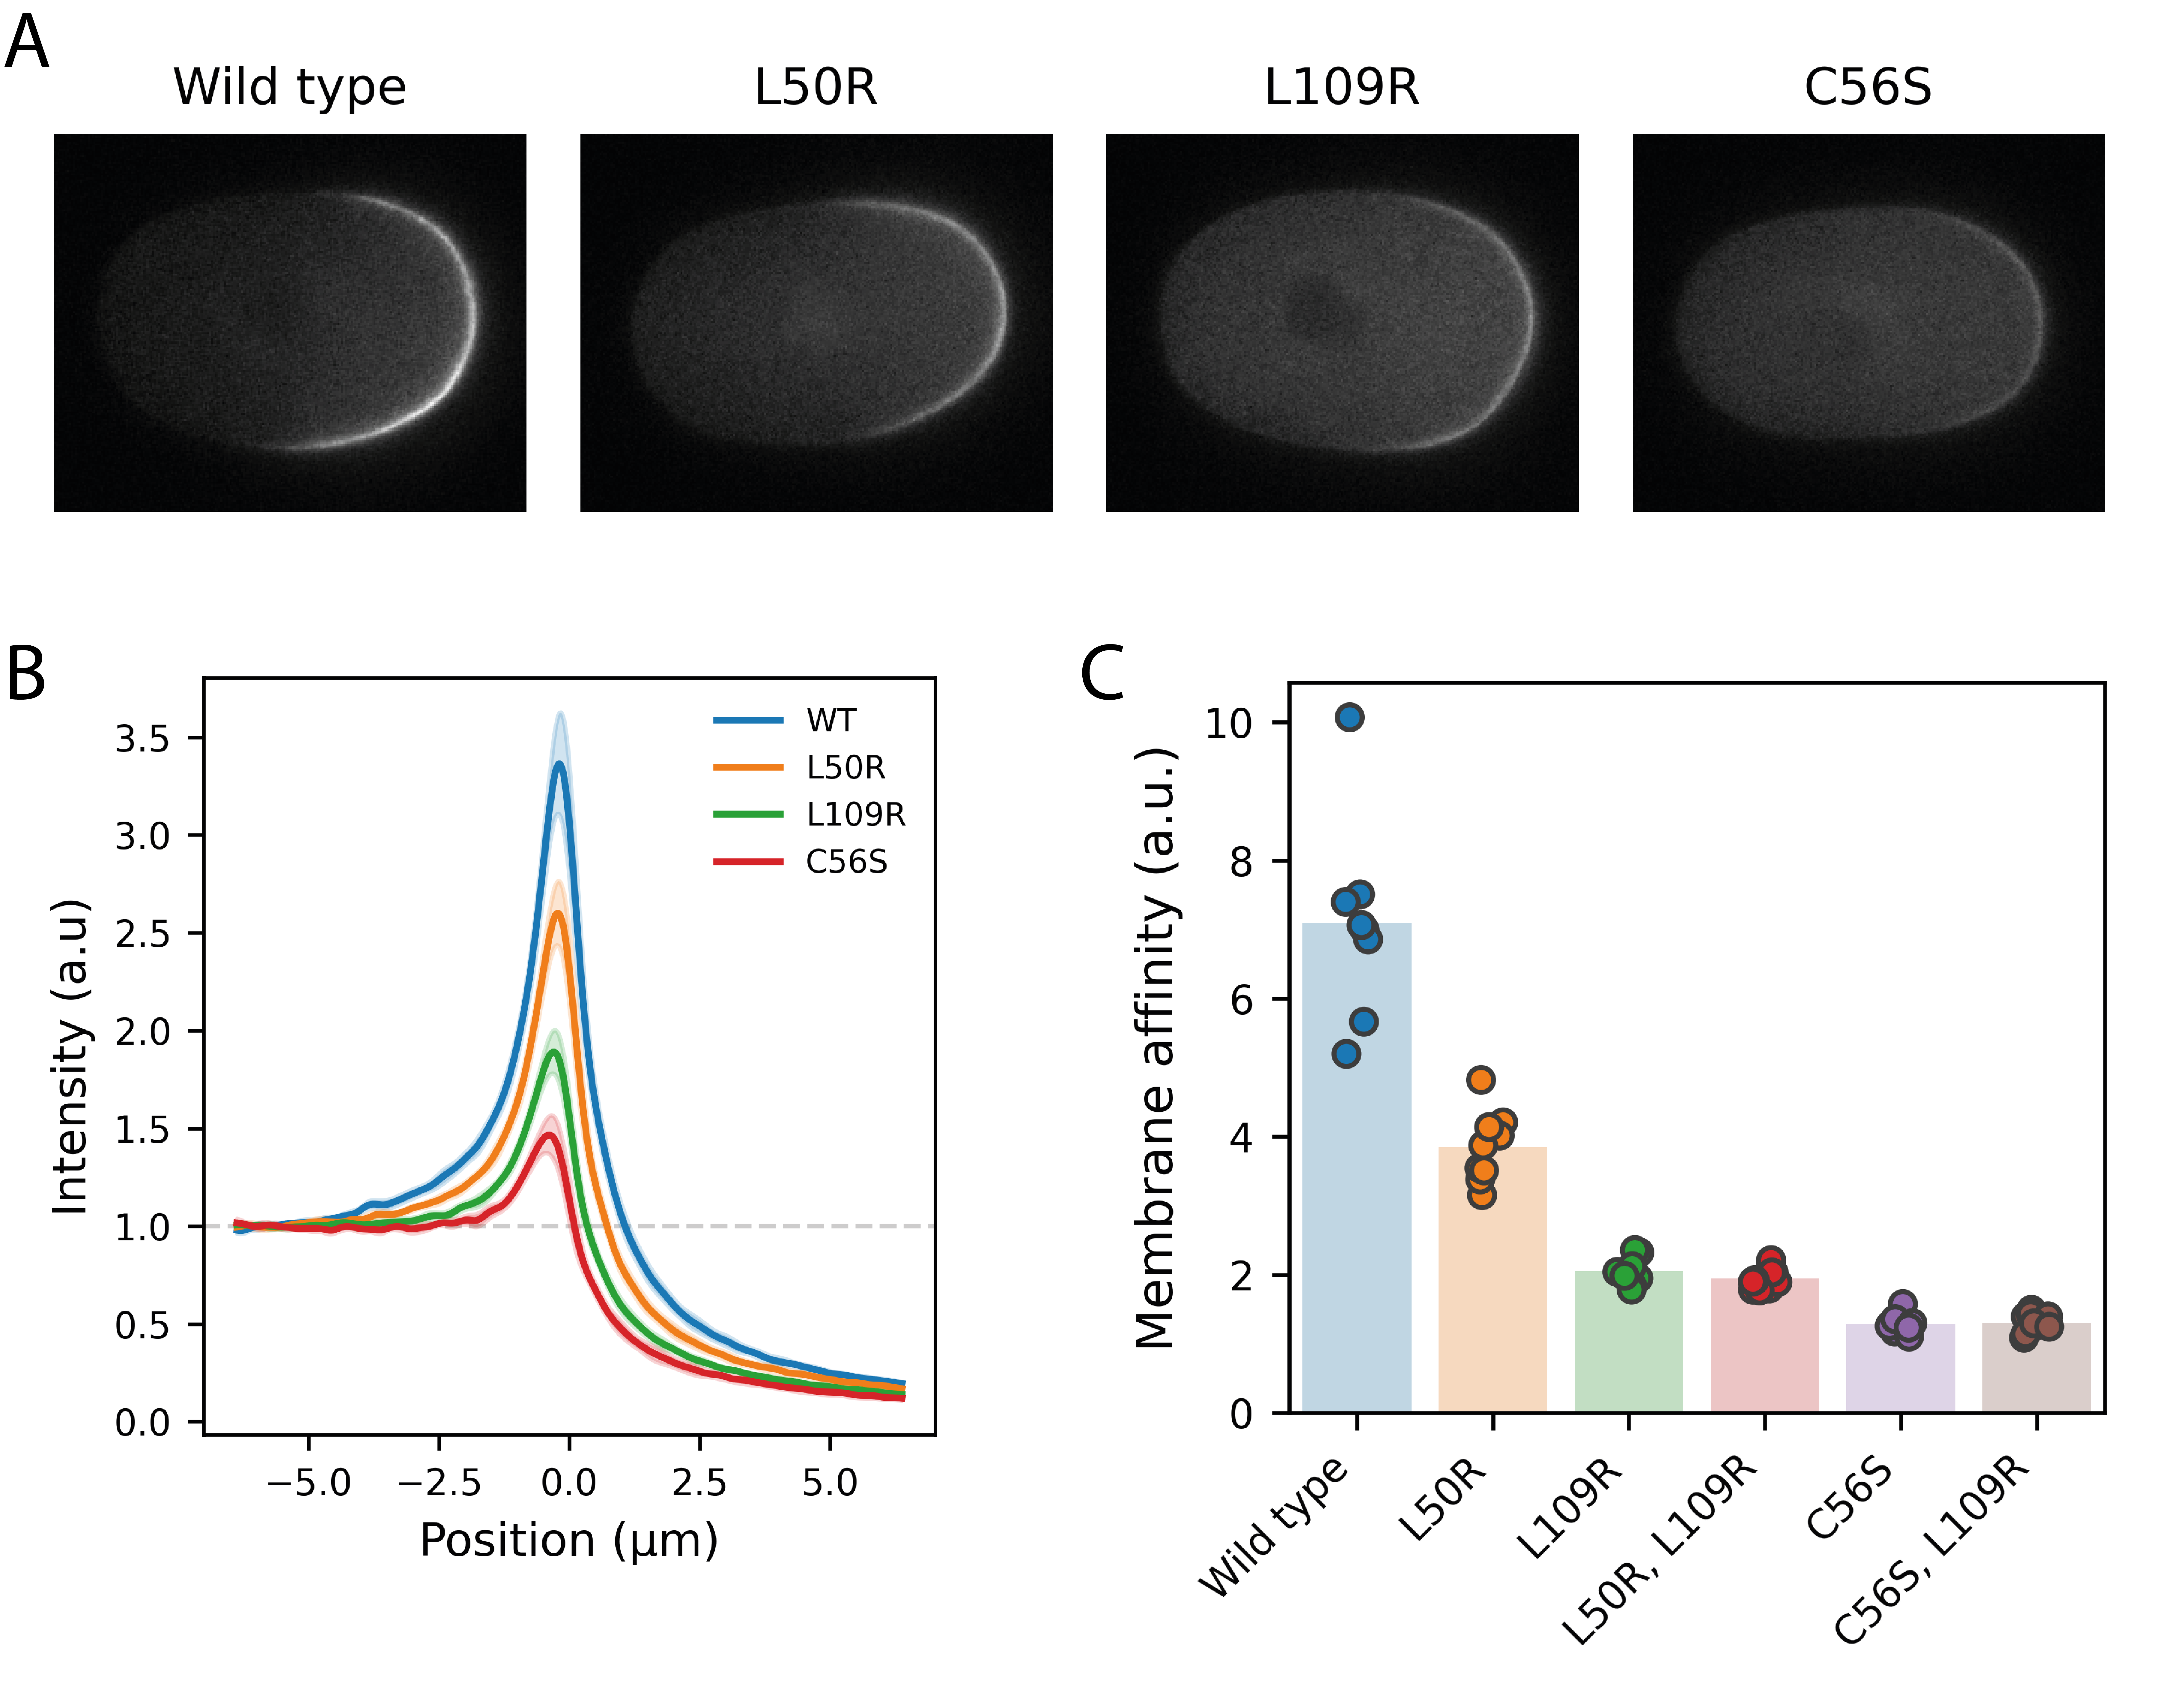
\includegraphics[scale=0.9]{dimer_interface_mutants_in_vivo}
\setlength{\abovecaptionskip}{20pt}
\centering
\mycaption{Title}{Caption}
\label{fig:dimer_interface_mutants_in_vivo}
\end{figure}

As shown in fig x, both mutations cause a strong reduction in affinity. This effect is stronger for L109R, which may suggest that L50R, whilst partially disrupting dimerisation, is insufficient to disrupt it completely. Combination of both mutants has no effect compared to L109R alone, indicating that dimerisation is completely disrupted in L109R. Interestingly, however, neither mutants reduce membrane affinity to the same extent as C56S. Assuming that dimerisation is fully disrupted by L109R, this implies that fully disrupting the domain may have additional effects compared to just disrupting dimerisation alone. One plausible explanation is that, in the case of C56S, the unfolded domain interferes with normal membrane binding, and therefore has an additional negative effect on membrane affinity. Compatible with this, a PH::RING fusion has lower overall membrane affinity that PH alone (fig x). Combining C56S and L109R has no effect compared to C56S alone, suggesting that dimerisation is completely disrupted in the C56S mutant.\\

\clearpage
\subsection{Discussion}


%%%%%%%%%%%%%%%%%%%%%%%%%%%%%%%%%%%%%%%%%%%%%%%%%%%%%%%%%%
\clearpage
\section{A thermodynamic model of PAR-2 dimerisation}

\textit{This section describes work performed in conjunction with David Zwicker}

\subsection{Model description}

%Might be worth having a glossary of terms: ideal solution, chemical potential, enthalpy, chemical system, chemical state, thermodynamic equilibrium, free energy, volume fraction

% Thermodynamic equilibrium puts constraints on the behaviour of a system, and allows us to accurately describe behaviour with a small number of easily interpretable parameters. In a multi-component chemical system, thermodynamic equilibrium is reached when all chemical components are at concentrations that have no tendancy to change with time, so that there are no overall changes in the properties of the system.

% Systems are described by a number of chemical components, each of which has an associated chemical potential
% Chemical potential describes
% Thermodynamic equilibrium is reached when all chemical components are at concentrations that have no tendancy to change with time, so that there are no overall changes in the properties of the system. This state is reached when the chemical potentials describing each species are all identical, such that movement of a particle between two states leads to no net change in overall energy of the system.


Consider, for example a simple chemical system in which material is exchanging between two states, $a$ and $b$:
\begin{center}
\ce{a <=> b}
\end{center}

Regardless of how the system is initiated, the system will eventually stabilise in a state where the forward and reverse reactions are equal, meaning that the concentrations of a and b will have no tenancy to change over time. Energetically speaking, this state is reached when the total free energy of the system ($F$) is minimised. When our system is at this minimum, the partial derivative of total energy with respect the the concentration of a must be equal to the equivalent partial derivative of b, meaning that any a to b reaction (or vice versa) will have no net impact on the overall energy energy of the system:
\begin{align}
\frac{dF}{da} = \frac{dF}{db}
\end{align}

These derivatives are more commonly referred to as the chemical potential of each species ($\mu_x$). Using ideal solution theory, this property can be described for each species, in $k_BT$ units, as:
\begin{align}
\mu_a &= \ln\phi_a - w_a\\
\mu_b &= \ln\phi_b - w_b
\end{align} 

where $\phi_a$ and $\phi_b$ represent the volume fraction occupied by species a and b respectively, and $w_a$ and $w_b$ are enthalpies associated with each state (a measure of how energetically favourable each state is). Since the total amount of material is conserved, we have the initial constraint that:
\begin{equation}
\phi_a + \phi_b = \phi
\end{equation}

where $\phi$ is a constant representing the total amount of material. As stated earlier, chemical equilibrium is reached when $\mu_a = \mu_b$. Thus, for a given total amount of protein ($\phi$), we can use our thermodynamic description to calculate $\phi_a$ and $\phi_b$ at equilibrium:
\begin{align}
\phi_a &= \frac{\phi}{1 + e^{w_b - w_a}}\\
\phi_b &= \frac{\phi}{1 + e^{w_a - w_b}}
\end{align}

We can also see from equations xxx that, at equilibrium, the following relationship must always we true:
\begin{equation}
\frac{\phi_a}{\phi_b} = e^{w_a - w_b}
\end{equation}

showing that, regardless of the total amount of protein, there is a constant ratio between the two states at equilibrium. (This is, of course, obvious just by looking at the chemical equation). The ratio that is reached will depend on the enthalpy terms associated with each state. Where $w_a > w_b$ more protein will end up in state a than state b, and vice versa (fig x).\\

\begin{figure}[!h]
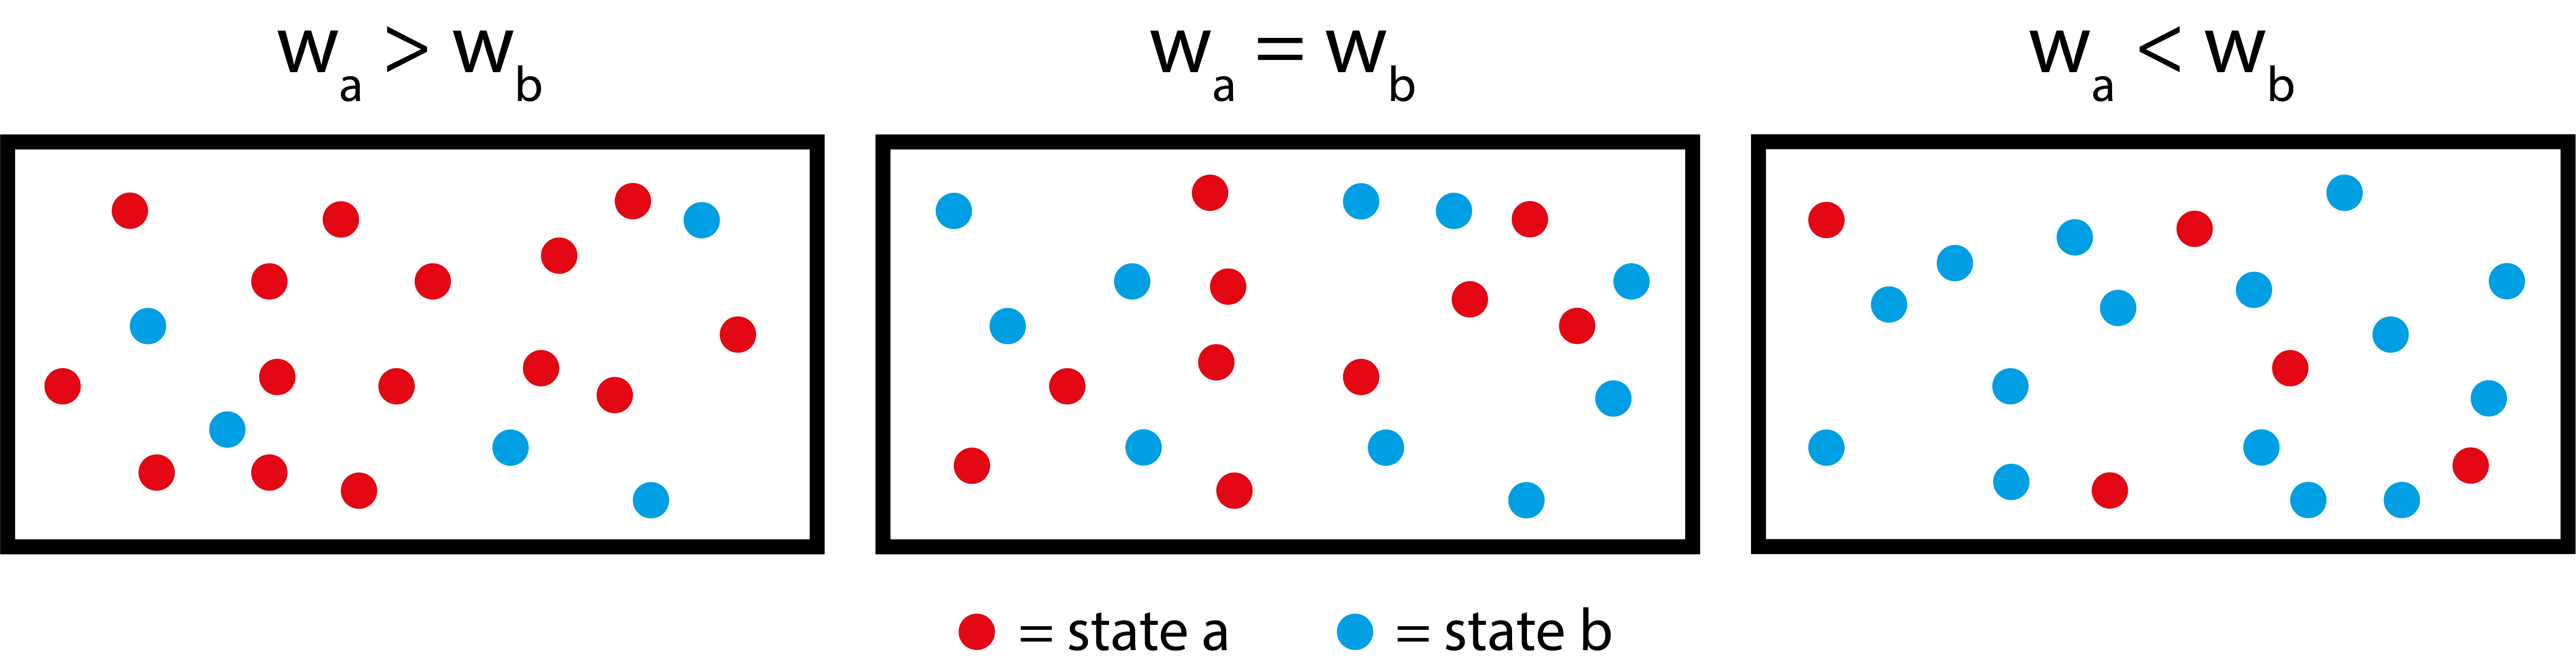
\includegraphics[scale=0.9]{thermodynamic_simple_example2}
\setlength{\abovecaptionskip}{20pt}
\centering
\mycaption{Title}{Caption}
\label{fig:thermodynamic_simple_example2}
\end{figure}

A similar description can apply to a species that is exchanging between two physical compartments. In this case a and b can represent protein in one of two spatial compartments, with $w_a$ and $w_b$ representing enthalpies associated with each compartment. The only difference is that the conservation of mass term must be slightly changed to account for potential differences in the volume of the two compartments. We will use:
\begin{equation}
\phi_a + \alpha\phi_b = \phi
\end{equation}

where $\alpha$ is a dimensionless exchange factor comparing the volume of the two compartments. (In this case $\phi$ can be interpreted as the volume fraction when all protein is in compartment a). As before, we end up with a linear relationship between concentrations in the two compartments, with ratios specified by $w_a - w_b$ (fig x - in this case, for simplicity, $\alpha = 1$).

\begin{figure}[!h]
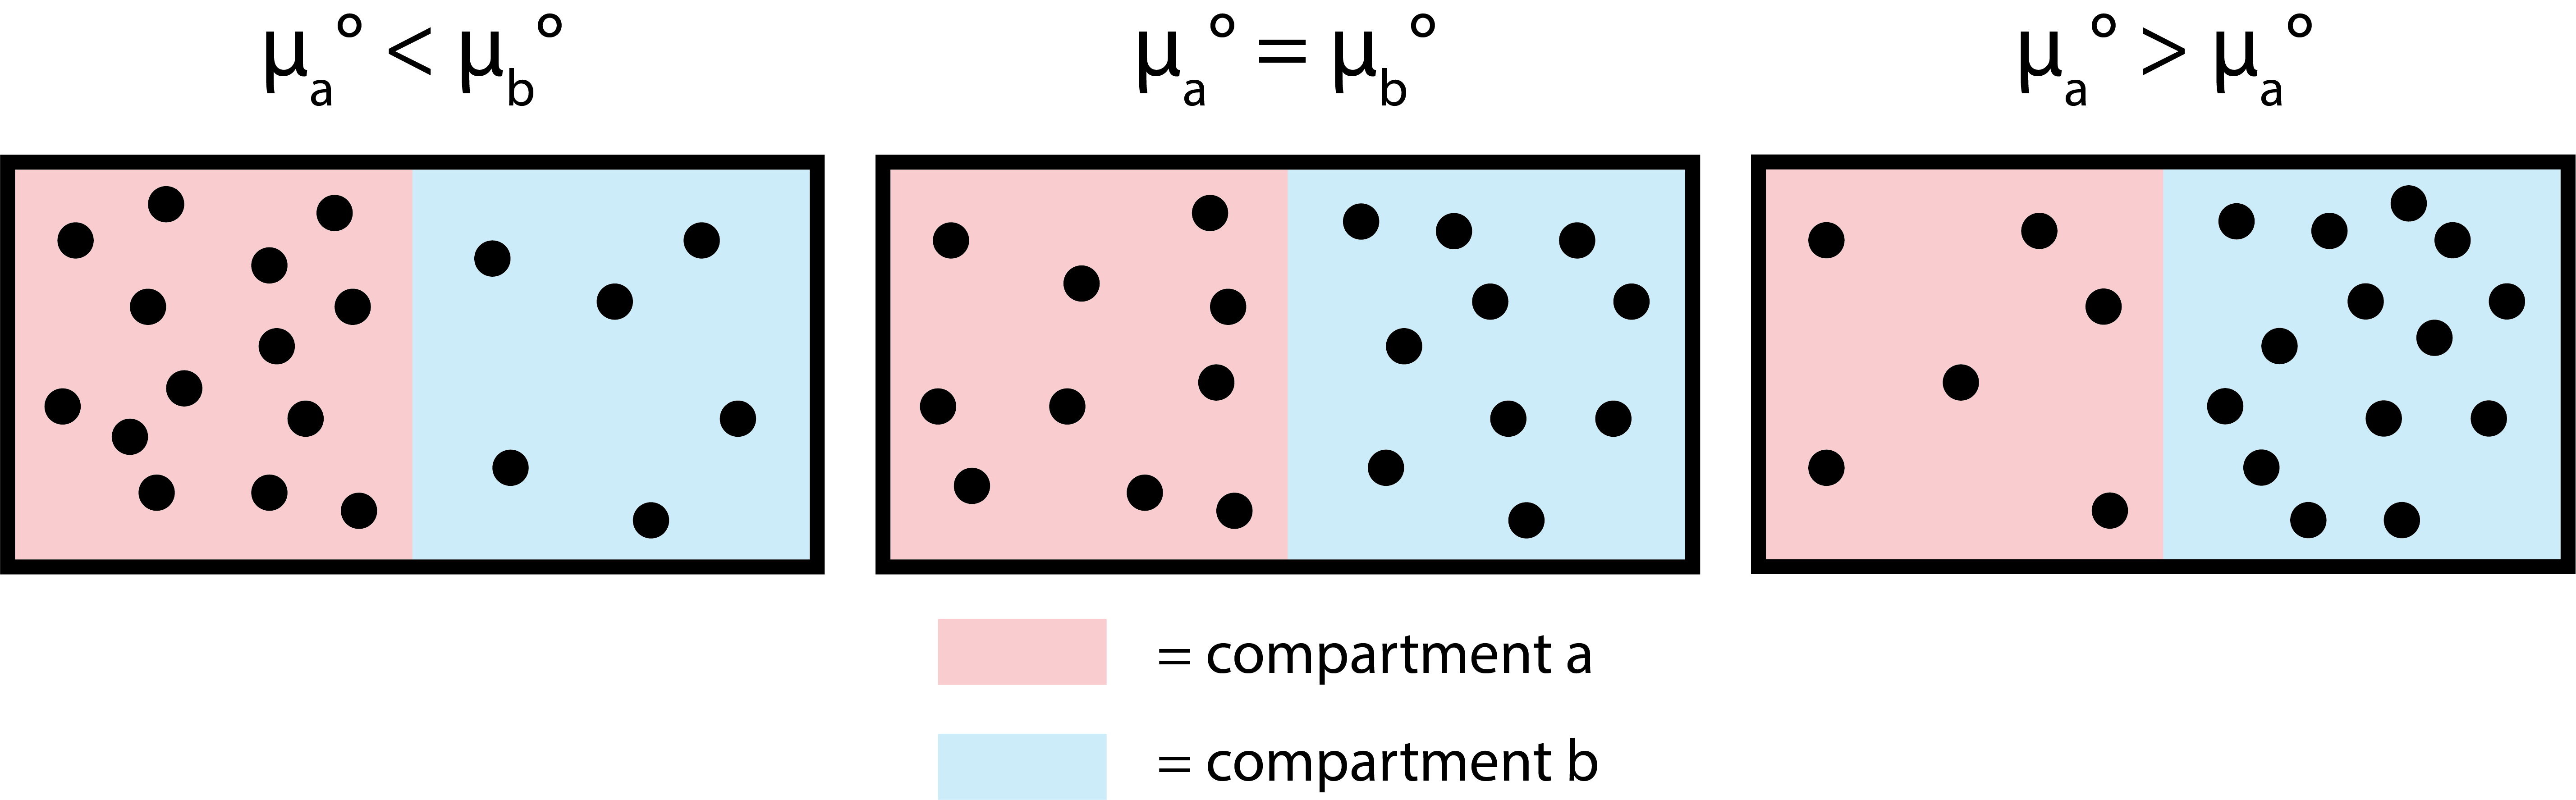
\includegraphics[scale=0.9]{thermodynamic_simple_example}
\setlength{\abovecaptionskip}{20pt}
\centering
\mycaption{Title}{Caption}
\label{fig:thermodynamic_simple_example}
\end{figure}

\subsubsection{Thermodynamic description of membrane binding}

We can use the same description for a particle exchanging between membrane bound and cytoplasmic pools (m and c), by considering membrane and cytoplasmic compartments as two volume compartments. In this case the membrane compartment can be described as a thin volume, characterised by a surface area and a (small) thickness. Since, as shown above, equilibrium concentrations are specified by the difference in enthalpy terms (rather than their absolute values), we can set $w_c = 0$, and define the chemical potentials as:
\begin{align}
\mu_c &= \ln\phi_c\\
\mu_m &= \ln\phi_m - w_m
\end{align} 

where $w_m$ can be interpreted as the membrane insertion energy (i.e. membrane affinity). The total amount of material is described as:
\begin{equation}
\phi_c + \alpha\phi_m = \phi
\end{equation}

where $\alpha$ (the volume ratio between the compartments) will be some small number $<<1$. Thus, as before, membrane concentrations at equilibrium can be described as a linear function of cytoplasmic concentrations, the slope of which will depend on $w_m$.\\

\subsubsection{Thermodynamic description of dimerisation}

We can extend the same analysis to consider a species dimerising:

\begin{center}
\ce{2x_1 <=> x_2}
\end{center}

Chemical potentials are can be described as:
\begin{align}
\mu_{x,1} &= \ln\phi_{x,1}\\
\mu_{x,2} &= \ln\phi_{x,2} - w_d
\end{align} 

with $w_d$ represents the dimerisation energy. Thermodynamic equilibrium is reached when $2\mu_{x,1} = \mu_{x,2}$ (the factor of 2 accounting for the differing stoichiometry between the two species), leading to the following relationship:
\begin{equation}
\frac{\phi_{x,2}}{(\phi_{x,1})^2} = e^{w_d}
\end{equation}

Thus, as concentrations of dimeric protein will vary linearly with the square of monomer concentrations (fig xA) (again, this is obvious from the chemical equation), and so the fraction of protein in the dimeric state will increase as total protein amounts increase (fig xB). Additionally, with the constraint that $\phi_x = \phi_{x,1} + \phi_{x,2}$ we can derive relationships for the concentrations of monomer and dimer as a function of total protein:
\begin{align}
\phi_{x,1} &= \frac{1}{2}e^{-w_d}\left(\sqrt{4e^{w_d}\phi_x + 1} - 1\right)\\
\phi_{x,2} &= \phi_x - \frac{1}{2}e^{-w_d}\left(\sqrt{4e^{w_d}\phi_x + 1} - 1\right)
\end{align}
% check equations

\begin{figure}[!h]
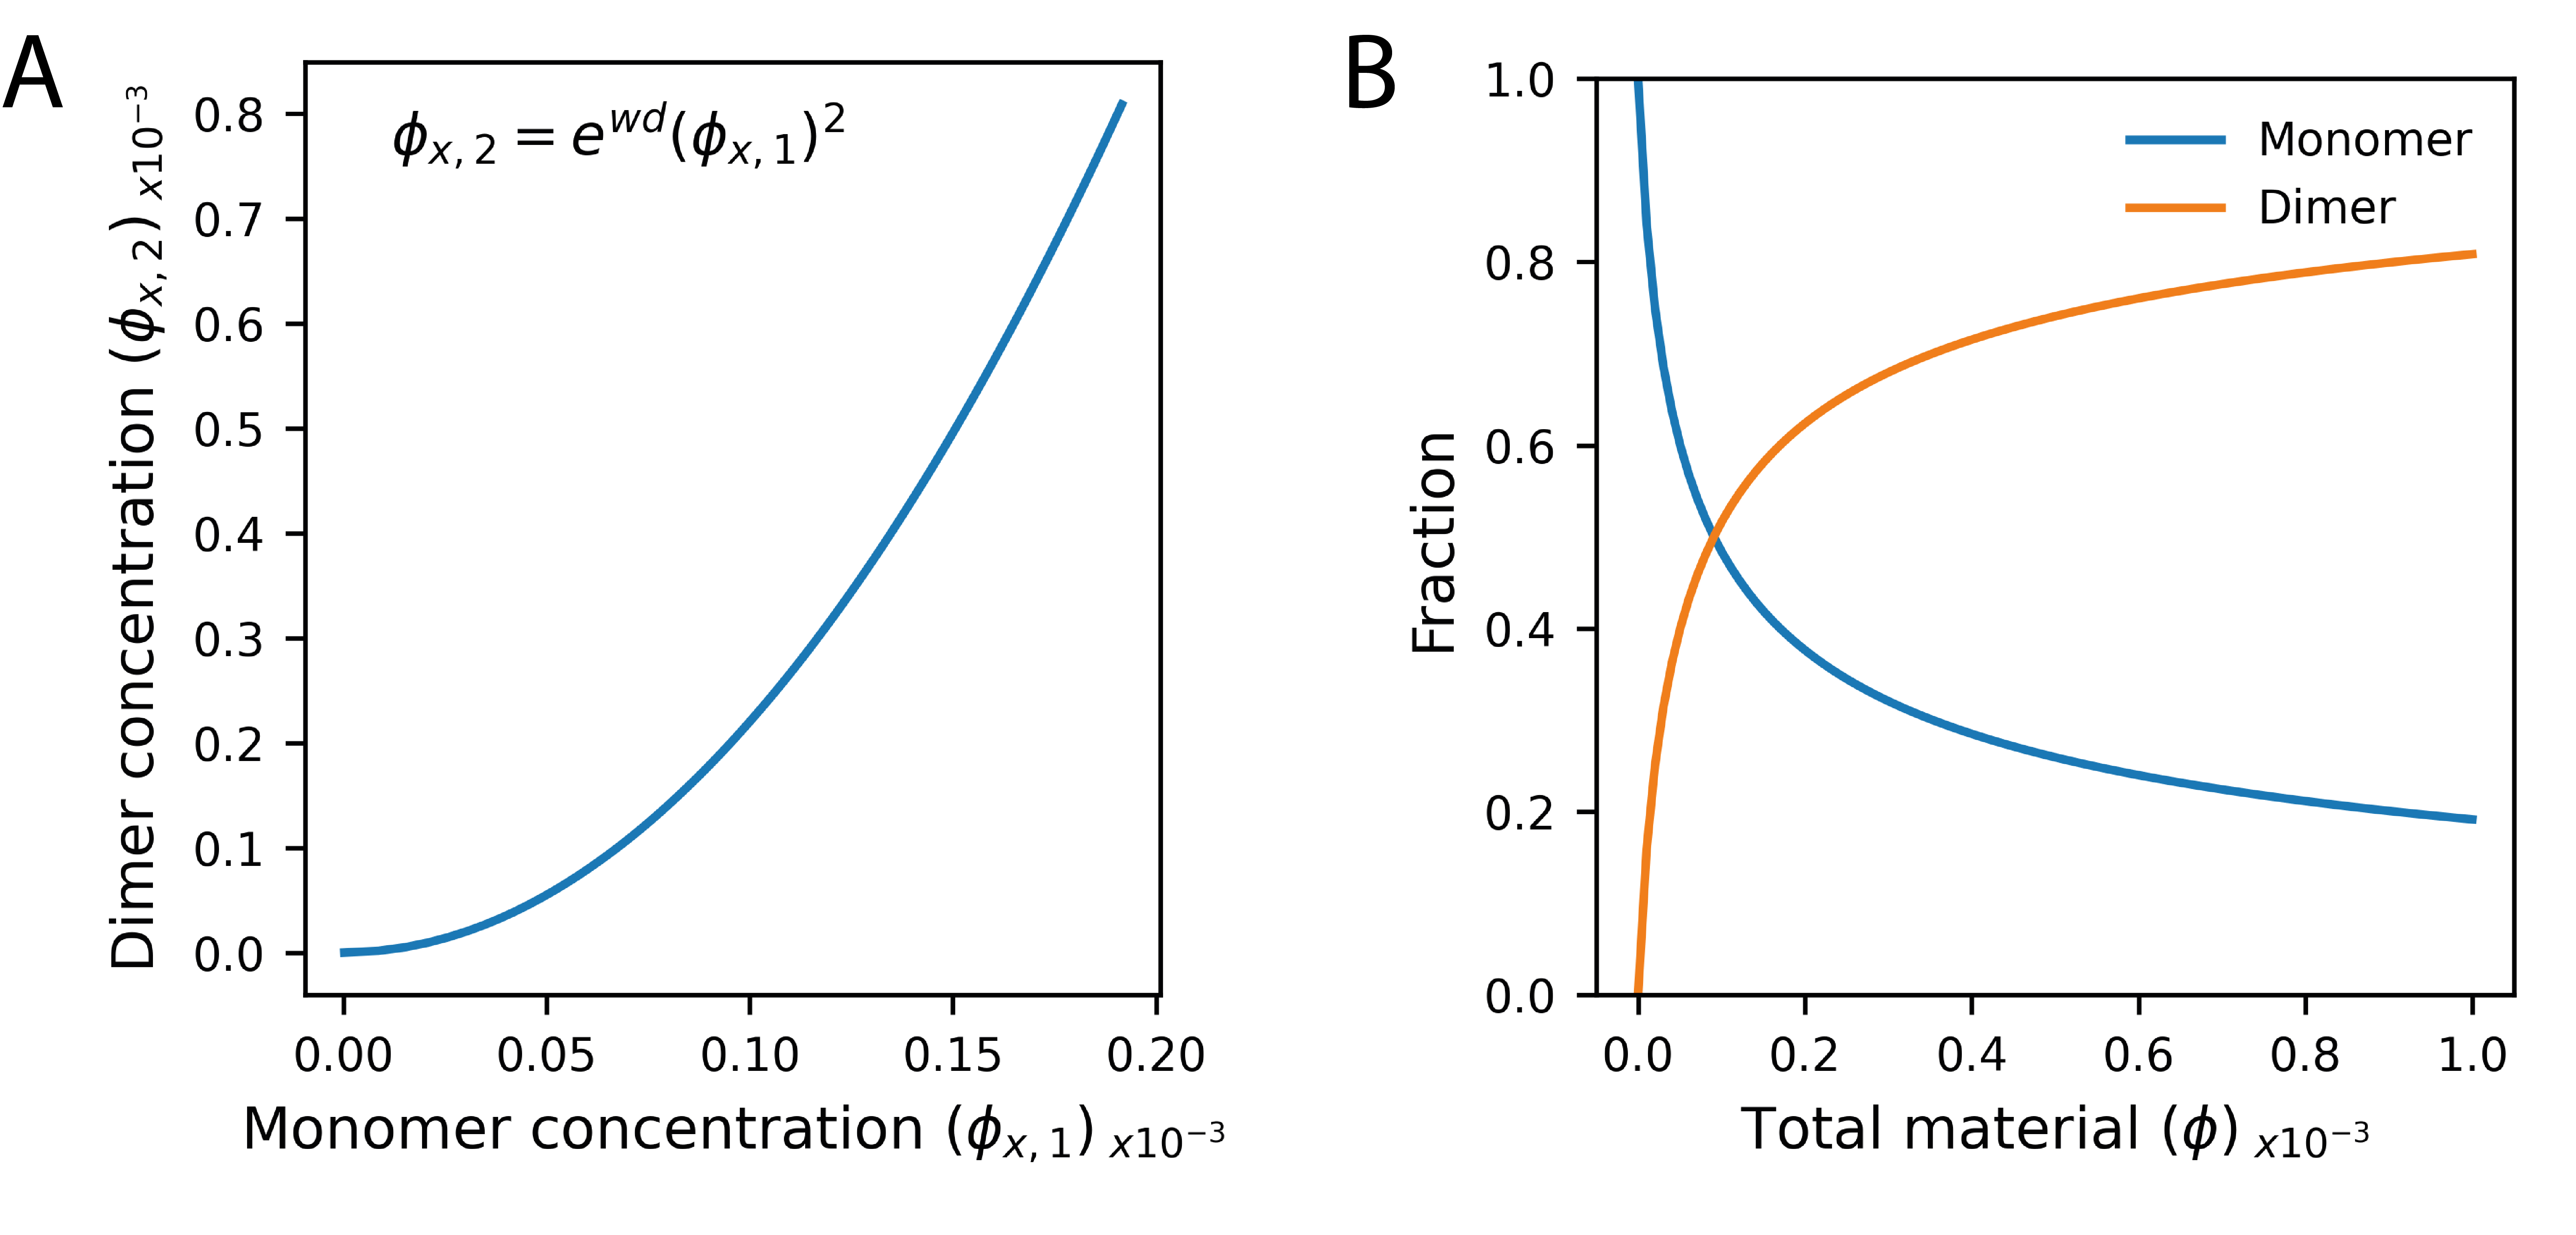
\includegraphics[scale=1]{thermodynamic_simple_dimer}
\setlength{\abovecaptionskip}{20pt}
\centering
\mycaption{Title}{Caption}
\label{fig:thermodynamic_simple_dimer}
\end{figure}


\subsubsection{4-species dimerisation model}

I next consider the case in which both dimerisation and membrane exchange are occurring. In this case, there are four potential species to consider: membrane monomers, membrane dimers, cytoplasmic monomers and cytoplasmic dimers (fig x). We can describe chemical potentials for the four species as:
\begin{align}
\mu_{c,1} &= \ln(\phi_{c,1}) - w_{c,1}\\
\mu_{c,2} &= \ln(\phi_{c,2}) - w_{c,2}\\
\mu_{m,1} &= \ln(\phi_{m,1}) - w_{m,1}\\
\mu_{m,2} &= \ln(\phi_{m,2}) - w_{m,2}
\end{align}

where $w_x$ represents the energy for each species. As only the differences in energies are important we set $w_{c,1} = 0$, and describe the four energies as:
\begin{align}
w_{c,1} &= 0\\
w_{c,2} &= w_d\\
w_{m,1} &= w_m\\
w_{m,2} &= 2w_m + w_d
\end{align}

where $w_d$ represents the energy gain upon dimerisation and $w_m$ the energy gain upon membrane association. Whilst the experimental data argues against significant dimerisation in the cytosol, there's no reason the believe that PAR-2 has an inability to dimerise in cytosolic conditions. Instead, it seems more likely that concentrations in the cytoplasm are just too low for this to happen. Thus, in the interest of simplicity, we are assuming that the dimerisation energy is equal in the membrane and cytoplasm. We also assume that the membrane association energy of a dimer is twice that of a monomer (as dimers have two binding interfaces). Thermodynamic equilibrium is reached when:
\begin{equation}
2\mu_{c,1} = \mu_{c,2} = 2\mu_{m,1} = \mu_{m,2}
\end{equation}

Since the total amount of material is conserved, we have:
\begin{align}
\phi &= \phi_c + \alpha\phi_m
\end{align}

where $\phi_c = \phi_{c,1} + \phi_{c,2}$ and $\phi_m = \phi_{m,1} + \phi_{m,2}$. With constraints imposed by mass conservation, equation x can be solved analytically to obtain expressions for each of the four species as a function of $\phi$. Figure x shows that, for a fixed total amount of protein, the equilibrium fraction of total protein in each of the four states will vary depending on the two energy parameters. With low $w_d$ and low $w_m$ protein will largely by cytoplasmic and monomeric; with low $w_d$ and high $w_m$ protein will be largely membrane-bound and monomeric; with high $w_d$ and low $w_m$ protein will be largely cytoplasmic and dimeric; and with high $w_d$ and high $w_m$ protein will be largely membrane-bound and dimeric. At intermediate energies a mix of states can be observed.\\

\begin{figure}[!h]
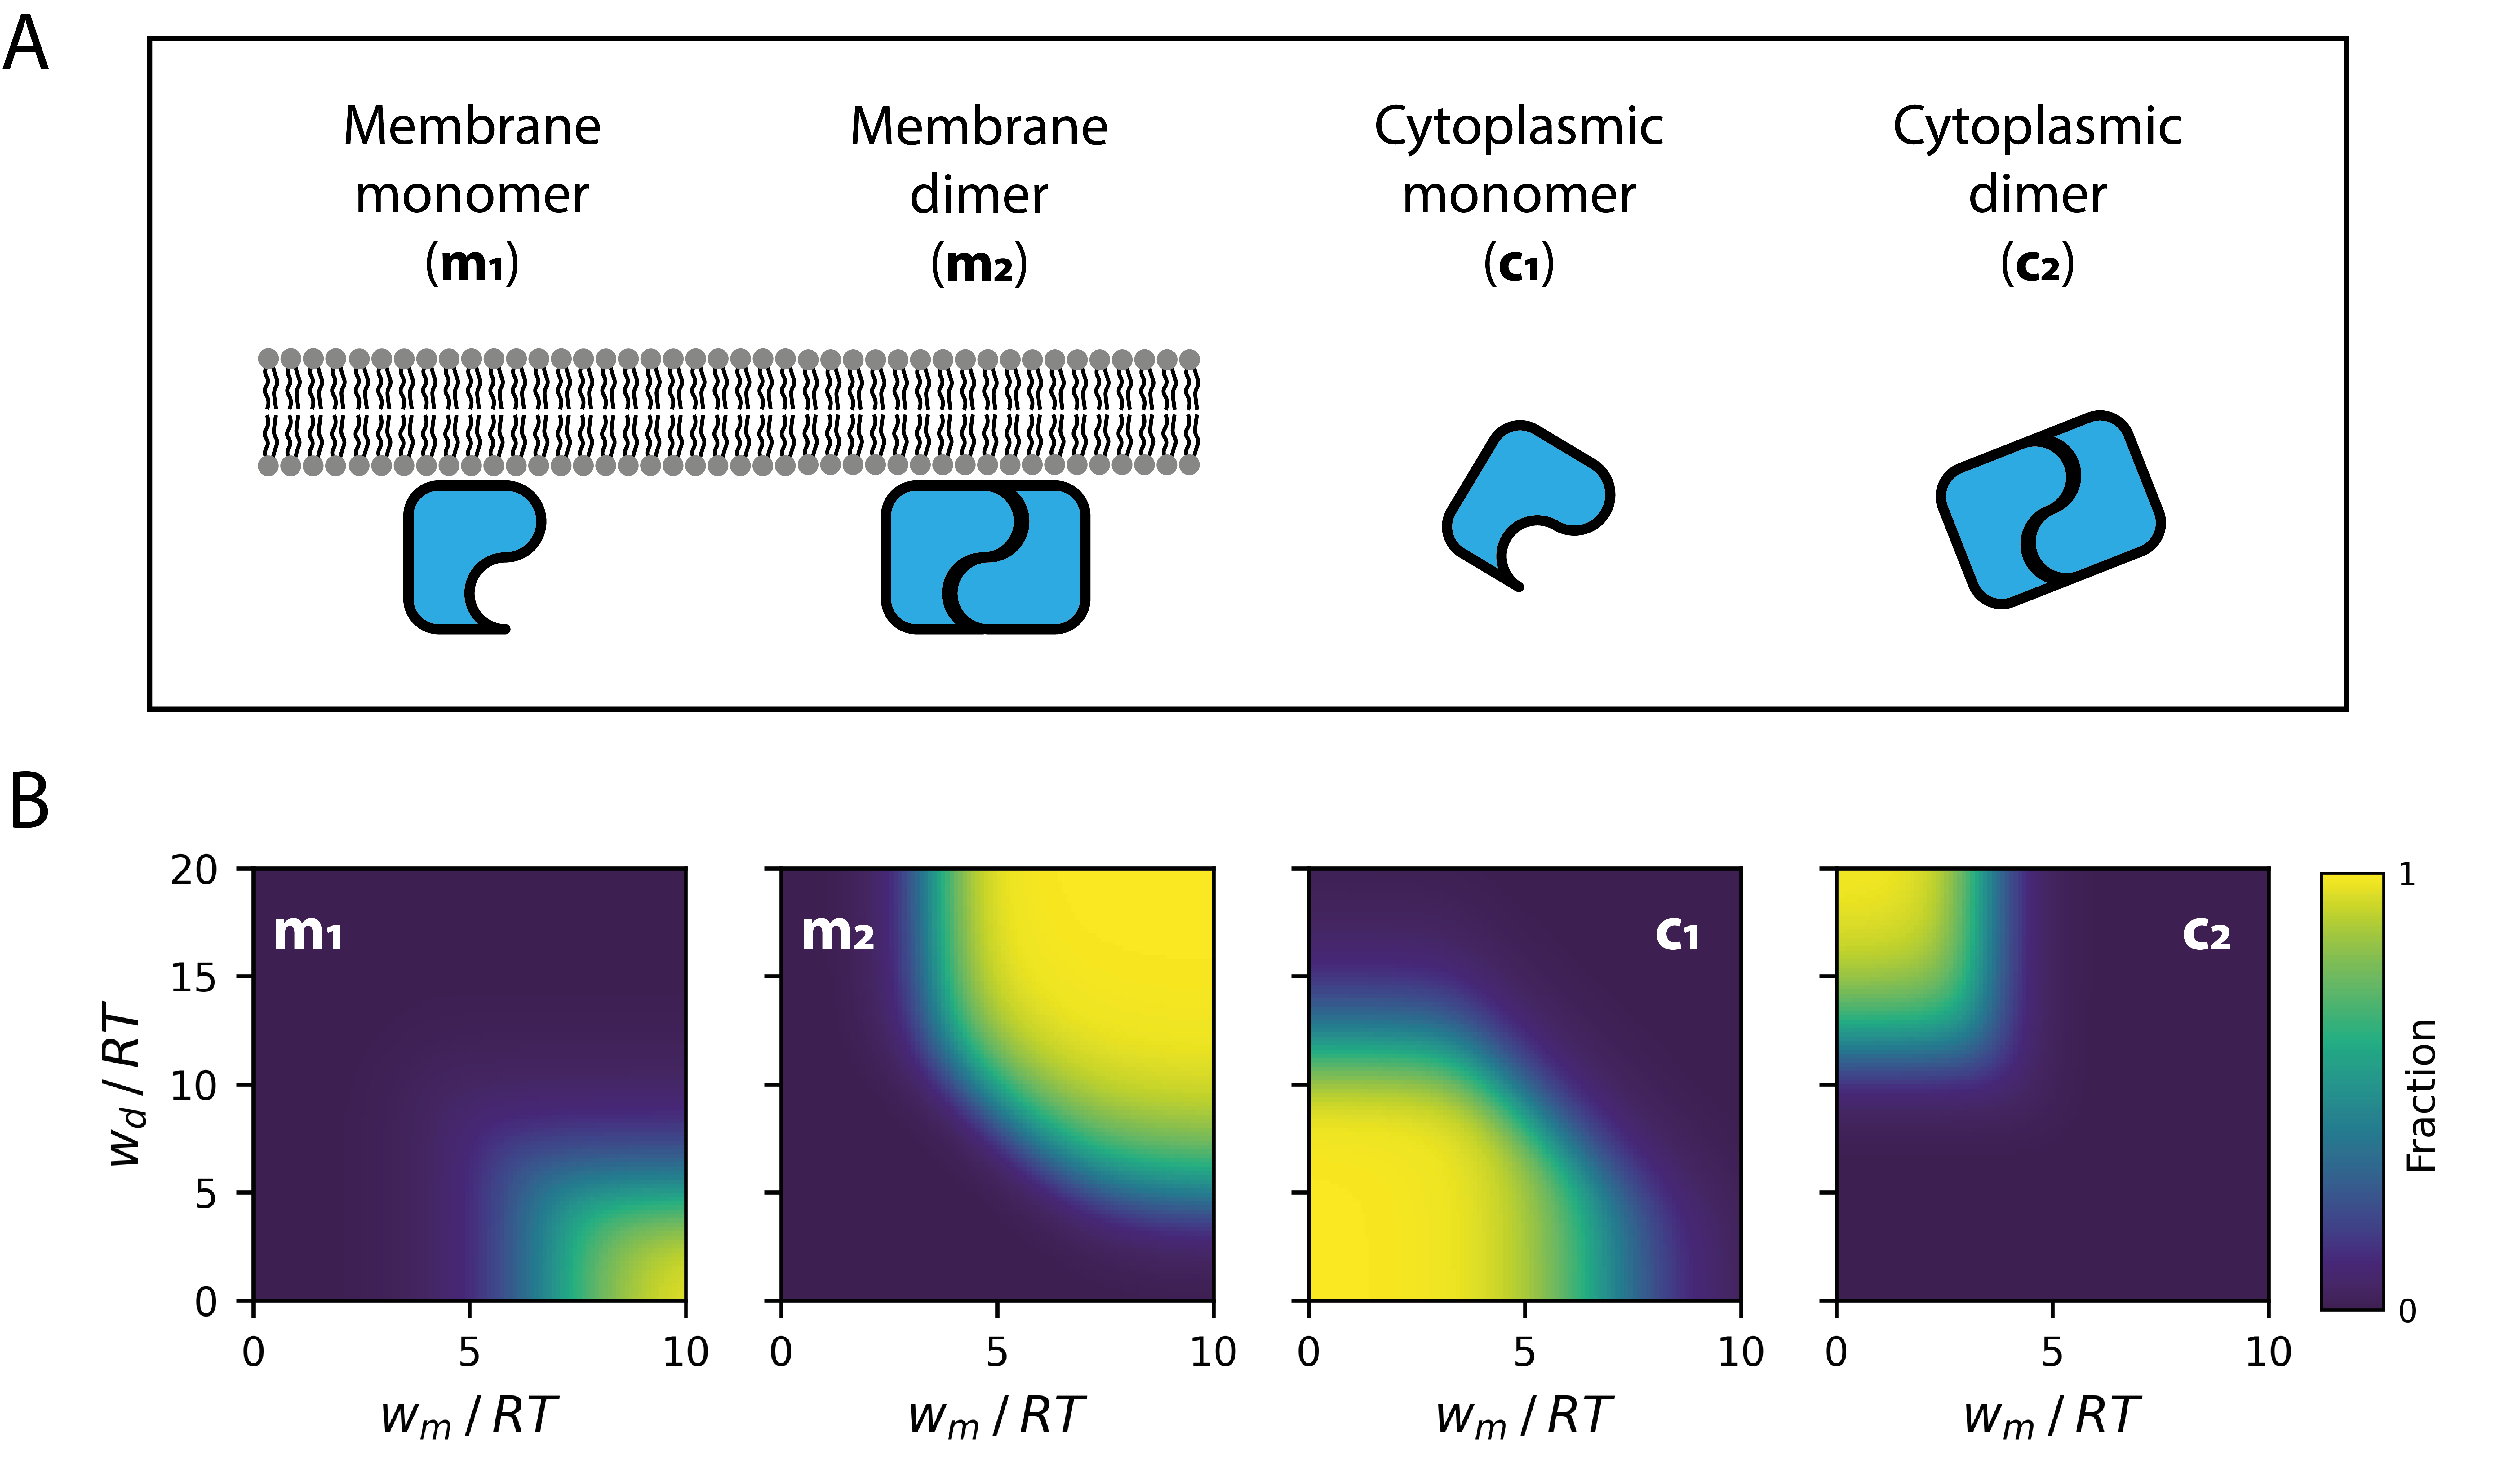
\includegraphics[scale=0.9]{thermodynamic_model_species}
\setlength{\abovecaptionskip}{20pt}
\centering
\mycaption{Title}{Caption}
\label{fig:thermodynamic_model_species}
\end{figure}


\subsection{Dimerisation-driven positive feedback}

Given the nonlinearities associated with dimerisation reactions, the distribution of protein between the four states is expected to vary depending on total protein amounts. This is particularly interesting in the case of PAR-2, as partitioning between the cytoplasm and membrane doesn’t follow simple linear kinetics, but varies depends on dosage (section x). I therefore investigated whether our simple thermodynamic behaviour can capture similar behaviour, by varying $\phi$ across a range of concentrations and solving for $\phi_m$ and $\phi_c$. \\

Figure x shows that, in certain parameter regimes, clear nonlinearity can be observed. For a given value of $w_m$, changing $w_d$ impacts both the shape and the amplitude of the cytoplasm vs membrane relationship (fig xA). By stabilising the high affinity dimeric state, increases to $w_d $increase overall membrane affinity for a constant $w_m$, leading to a steeper relationship. \\

\begin{figure}[!h]
% possibly include affinity vs dosage panels
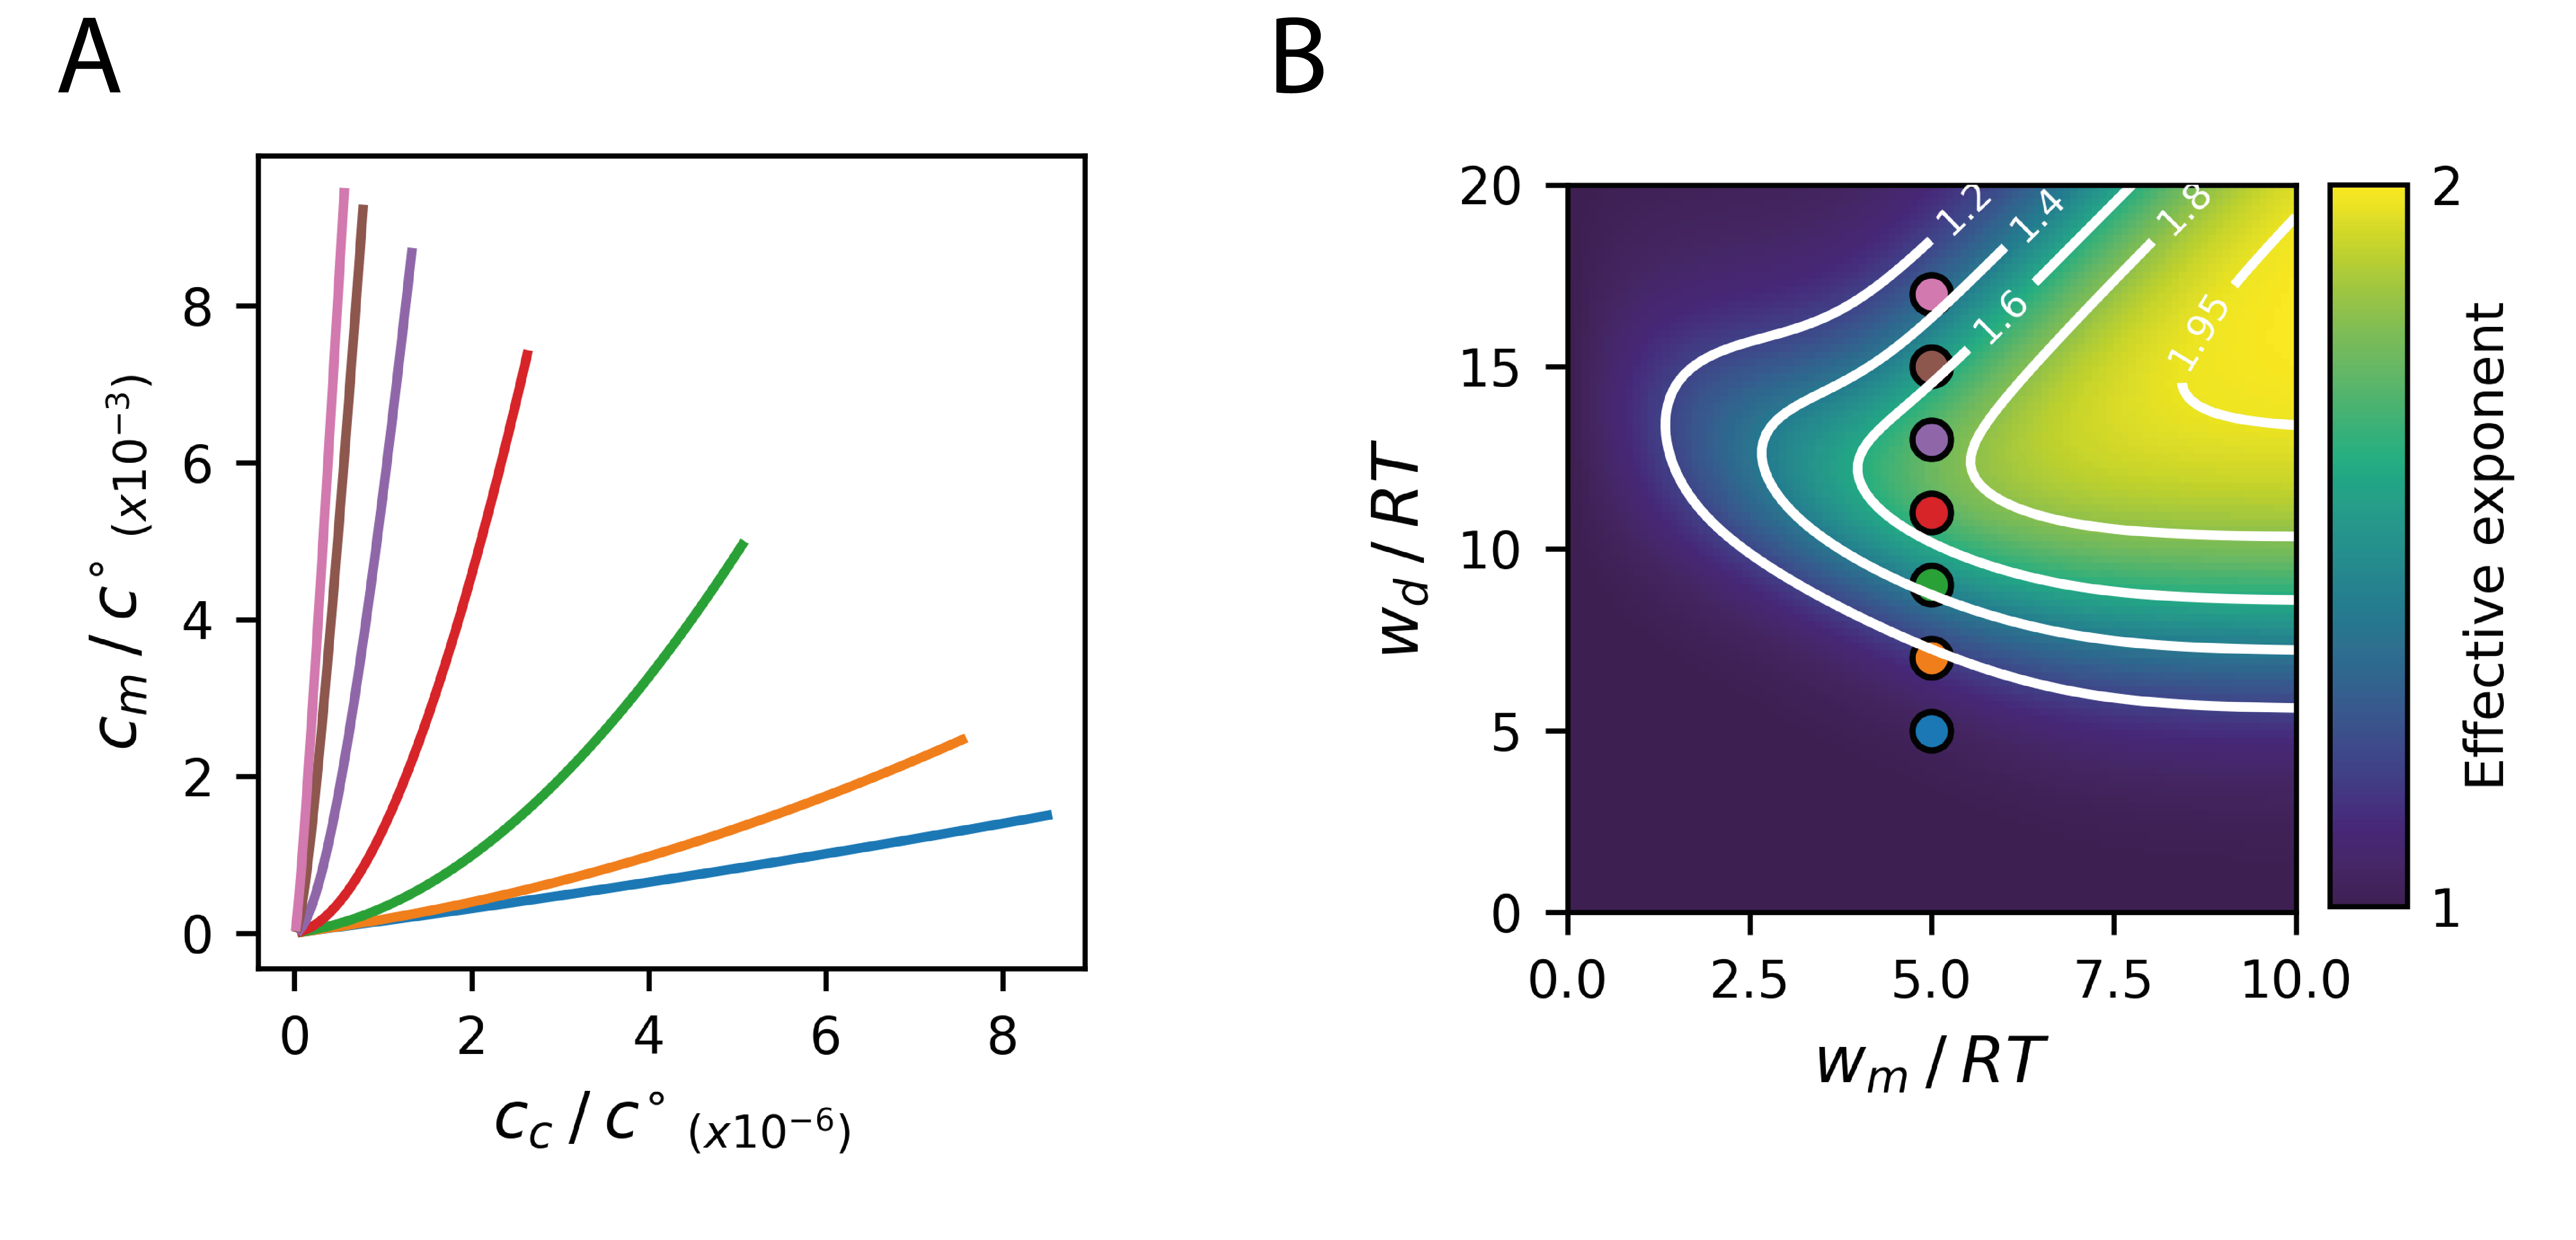
\includegraphics[scale=1]{thermodynamic_model_feedback}
\setlength{\abovecaptionskip}{20pt}
\centering
\mycaption{Title}{Caption}
\label{fig:thermodynamic_model_feedback}
\end{figure}

As shown in fig xB, effective exponent of the cytoplasm vs membrane relationship ($\beta$), obtained by fitting $\phi_m = \alpha \phi_c^{\beta}$, varies across parameter space between 1 (linear relationship) and 2 (quadratic relationship). Peak nonlinearity occurs in regions of high membrane energy and intermediate dimerisation energy. This corresponds to regions of parameter space in which membrane protein is largely dimeric and cytoplasmic protein largely monomeric, across the relevant range of dosages (fig x). Where $w_d$ is low, protein is unable to dimerise, even at enriched membrane concentrations, and so the model simple linear kinetics like described in section x. If, on the other hand, $w_d$ is too high, protein is constitutively dimeric in both the membrane and cytoplasm, and will behave similarly to a monomer (albeit with a higher membrane affinity). If $w_d$ is intermediate, then an asymmetry is observed whereby protein is dimeric on the membrane but not in the cytoplasm, provided that $w_m$ is sufficiently large to set up a substantial concentration difference between the two compartments.\\

\begin{figure}[!h]
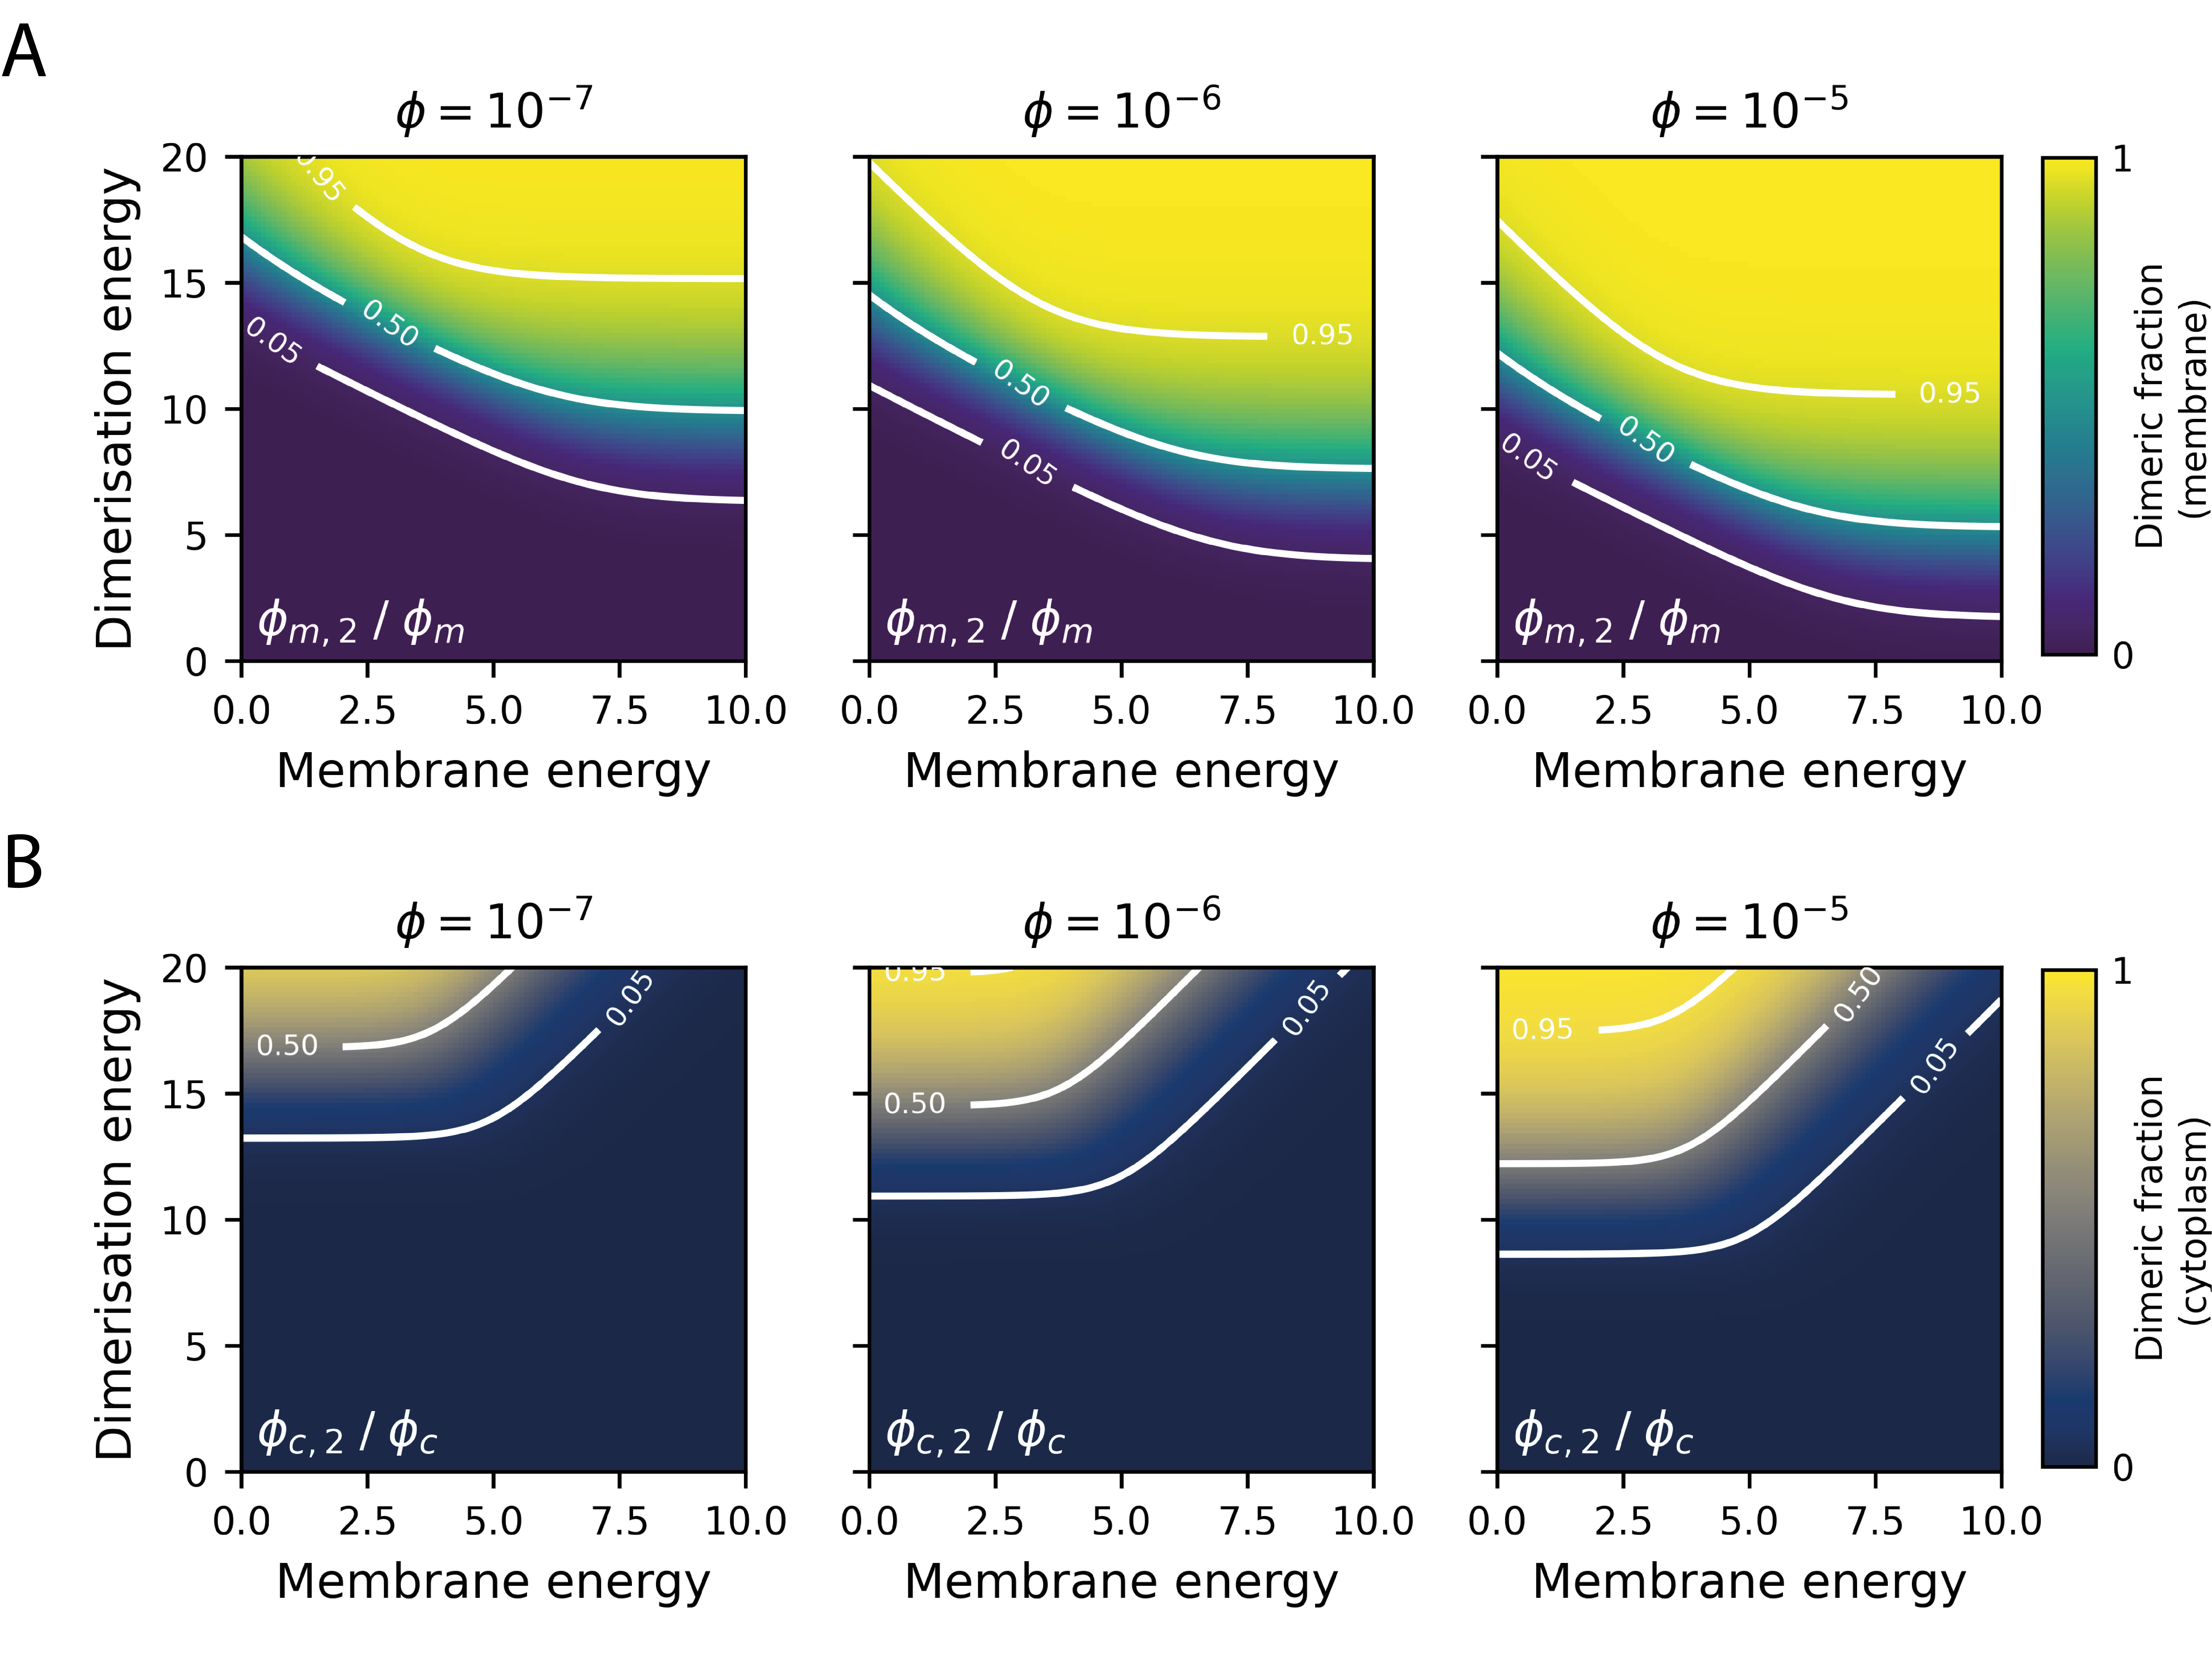
\includegraphics[scale=0.9]{thermodynamic_model_dimer_fractions}
\setlength{\abovecaptionskip}{20pt}
\centering
\mycaption{Title}{Caption}
\label{fig:thermodynamic_model_dimer_fractions}
\end{figure}

% Needs a comment here on why we get nonlinearity

%make the point here (or later) that this gives a linear increase in affinity, so is not expected to contribute to bistability

\clearpage
\subsection{Quantitative analysis of PAR-2 membrane binding kinetics in vivo}

% the above makes predictions about the quantitative relationship between membrane and cytoplasmic concentrations. Suggests no bistability. Contrasts with earlier results. Let's try and measure this in vivo

\subsection{Discussion}

% We have also considered non-ideal models and this doesn't change the behaviour within concentration ranges relevant to the in vivo measurements

%%%%%%%%%%%%%%%%%%%%%%%%%%%%%%%%%%%%%%%%%%%%%%%%%%%%%%%%%%
\clearpage
\section{Modelling dimerisation-driven positive feedback in the PAR network}

\subsection{Model description}

\subsubsection{Reducing thermodynamic model to a two-species model} 

To simplify further analysis, we can convert the four species thermodynamic model to a two species model, in which we only track overall membrane and cytoplasmic concentrations, $\phi_m$ and $\phi_c$, irrespective of dimeric state. If we assume that dimerisation reactions in the membrane and cytoplasm are fast relative to membrane binding, we can define instantaneous monomer and dimer concentrations as a function of overall concentration. For example, for cytoplasmic protein:
% check equations
\begin{align}
\phi_{c,1} &= \frac{1}{2}e^{-w_d}\left(\sqrt{4e^{w_d}\phi_c + 1} - 1\right)\\
\phi_{c,2} &= \phi_c - \frac{1}{2}e^{-w_d}\left(\sqrt{4e^{w_d}\phi_c + 1} - 1\right)
\end{align}

which is identical to the description in section x. As a result, and because we can describe the chemical potential of each of these species individually (equations xxx), we can combine expression <> and <> to define the overall chemical potential of cytoplasmic protein ($\mu_c$) as a function of overall cytoplasmic concentrations ($\phi_c$):
\begin{equation}
\mu_c = \ln(\phi_c) - \frac{1}{2}\ln\left(1 + 2e^{w_d}\phi_c + \sqrt{4e^{w_d}\phi_c + 1}\right)
\end{equation}
% check equation

And analogously for membrane bound protein: 
\begin{equation}
\mu_m = \ln(\phi_m) - \frac{1}{2}\ln\left(1 + 2e^{w_d}\phi_m + \sqrt{4e^{w_d}\phi_m + 1}\right) - w_m
\end{equation}
% check equation

These two equations can be solved analytically at equilibrium ($\mu_c$ = $\mu_m$) to find equilibrium membrane and cytoplasmic concentrations.


\subsubsection{Explicit description of membrane binding kinetics} 

Building kinetic models requires a description of membrane and unbinding rates, rather than just energetics. Exchange can be written as:

\begin{center}
\ce{$\phi_c$ <=>[$k_{on}$][$k_{off}$] $\phi_m$}
\end{center}

For a given composition, flux on ($s_{on}$) is equal to $k_{on}\phi_c$, and flux off ($s_{off}$) is equal to $k_{off}\phi_m$. Using transition state theory, these fluxes can be written as:
\begin{align}
s_{on} &= ke^{\mu_c}\\
s_{off} &= ke^{\mu_m}
\end{align}

where $k$ is a kinetic factor. Using our previous descriptions of cytoplasmic and membrane chemical potentials, the kinetic rate constants can be calculated as:
\begin{align}
k_{on} &= \frac{k}{\sqrt{2e^{w_d}\phi_c+ 1}}\\
k_{off} &= \frac{ke^{-w_m}}{\sqrt{2e^{w_d}\phi_m+ 1}}
\end{align}

implying a dependence on both energies and concentrations. This is shown for $k_{off}$ in fig x. Fig xA shows off rates plot a function of membrane energy and dimerisation energy, for a given membrane concentration. We can also see (fig xB), the dependence of off rates on concentrations.

\begin{figure}[!h]
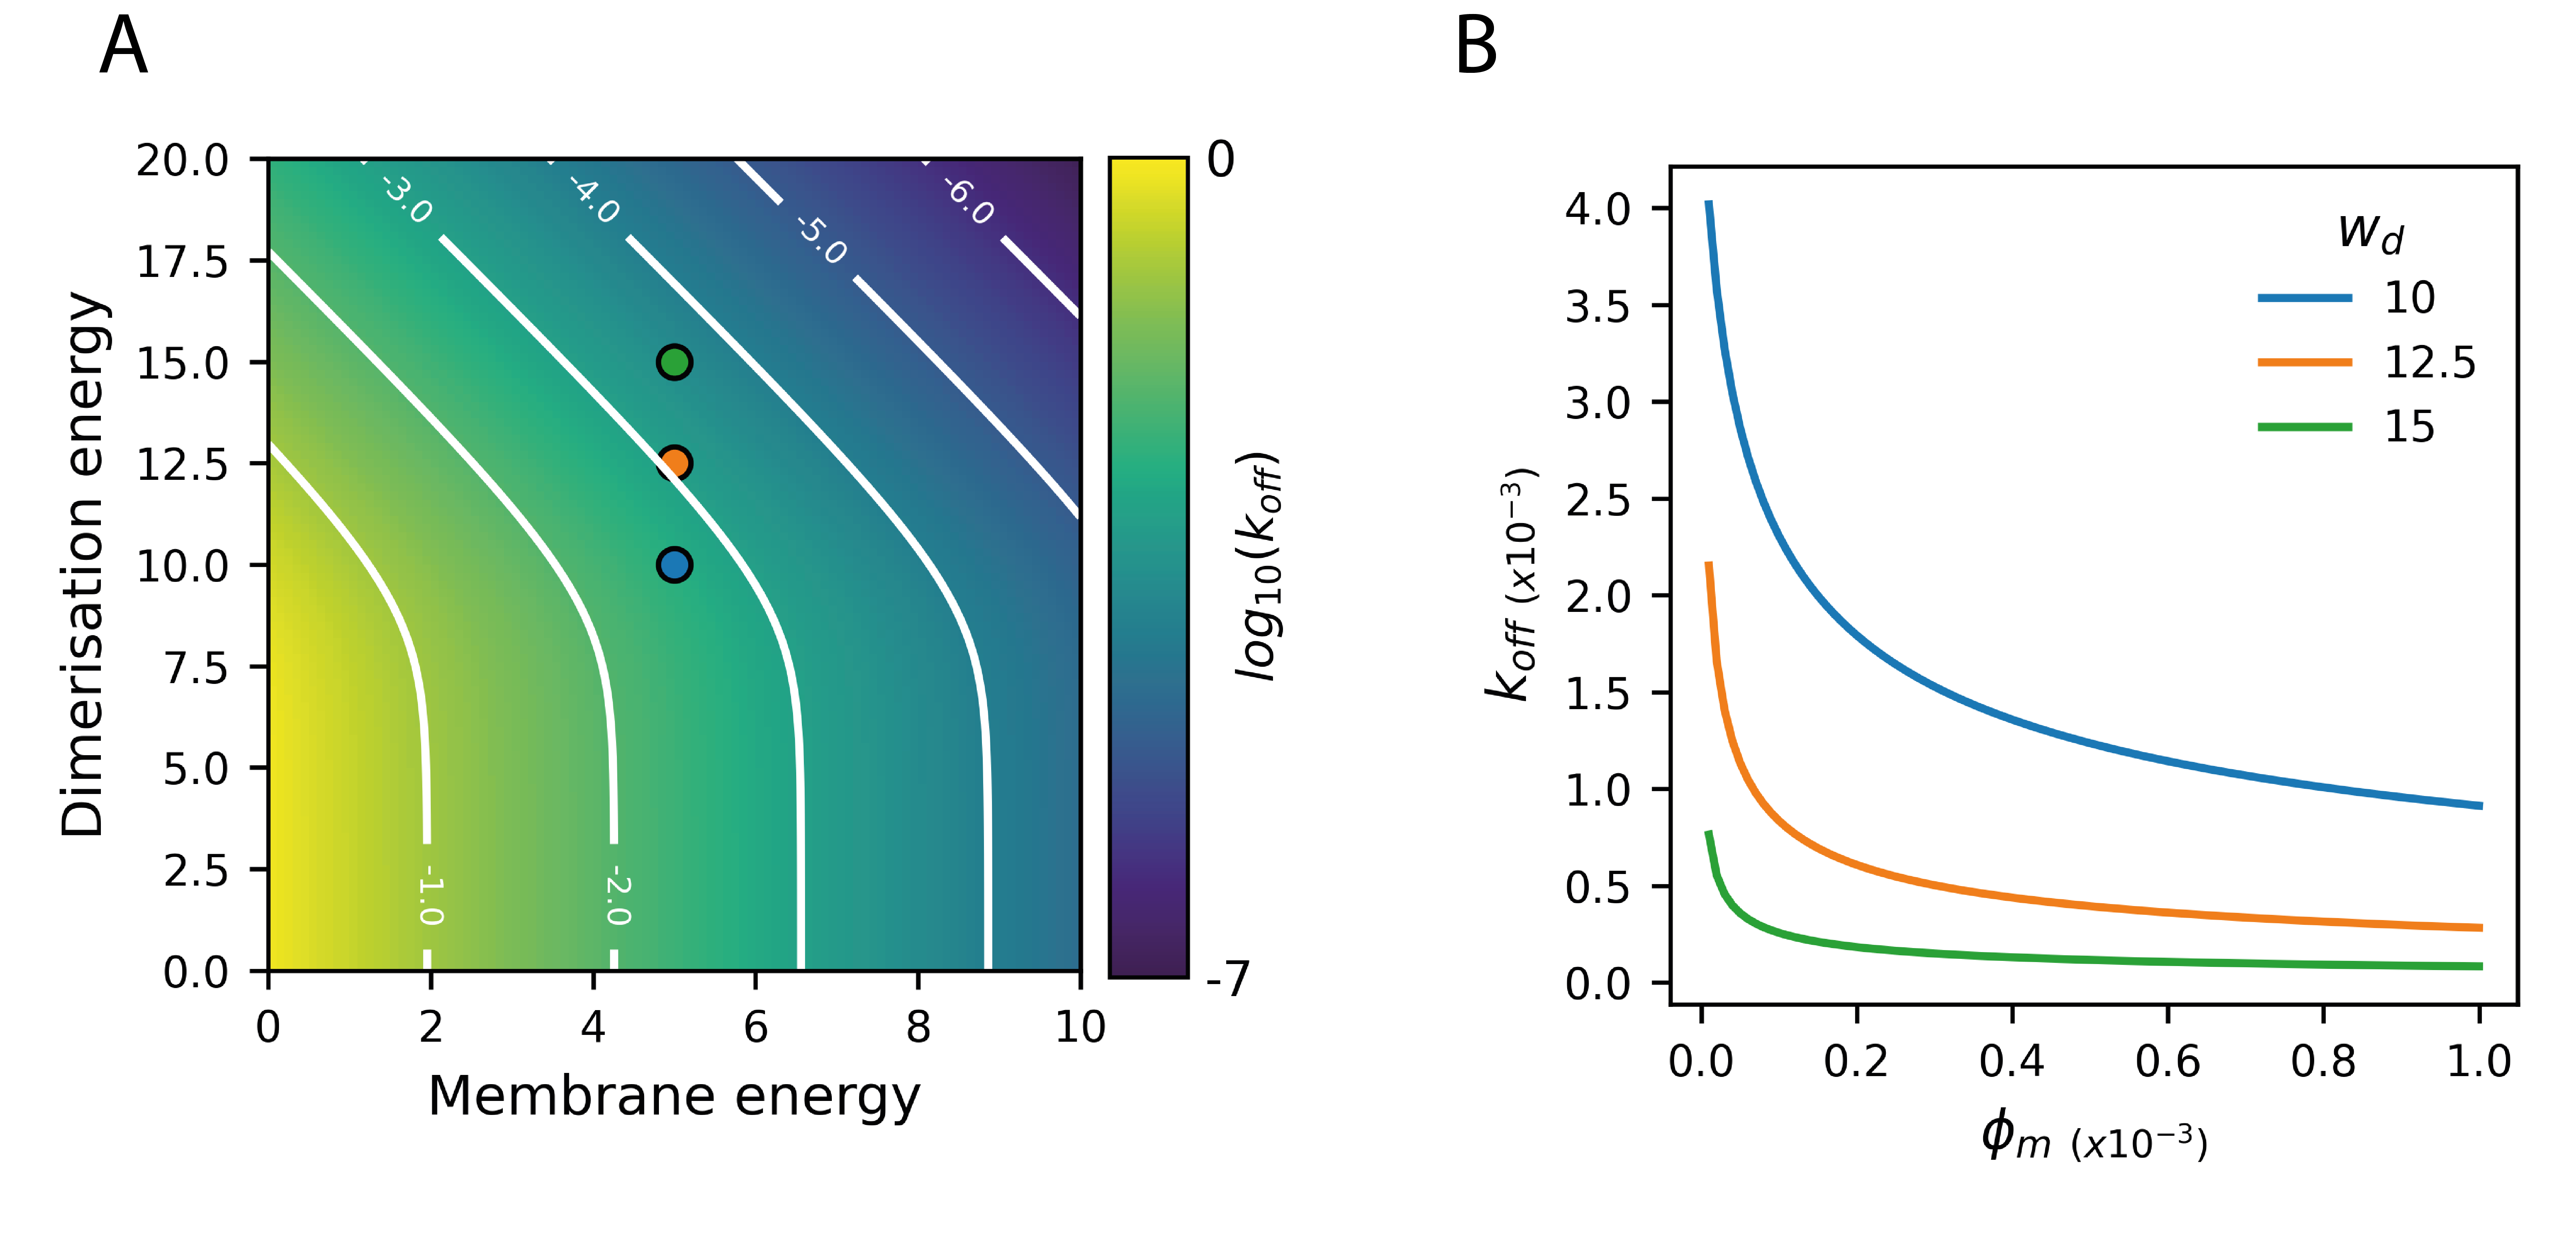
\includegraphics[scale=1]{thermodynamic_model_koff}
\setlength{\abovecaptionskip}{20pt}
\centering
\mycaption{Title}{Caption}
\label{fig:thermodynamic_model_koff}
\end{figure}

\subsubsection{Incorporation into mutual antagonism model}


%%%%%%%%%%%%%%%%%%%%%%%%%%%%%%%%%%%%%%%%%%%%%%%%%%%%%%%%%%
\clearpage
\section{Direct experimental manipulation of dimerisation}

\subsection{Forced constitutive dimerisation}

% Strikingly, we see the unexpected appearance of visible structures within the cell. Based on comparison to RAB localisation patterns, these appear to be endosomes.

% We also see the appearance of PAR-2 on the anterior membrane, suggesting that the protein is less susceptable to antagonism by PKC-3

\begin{figure}[!h]
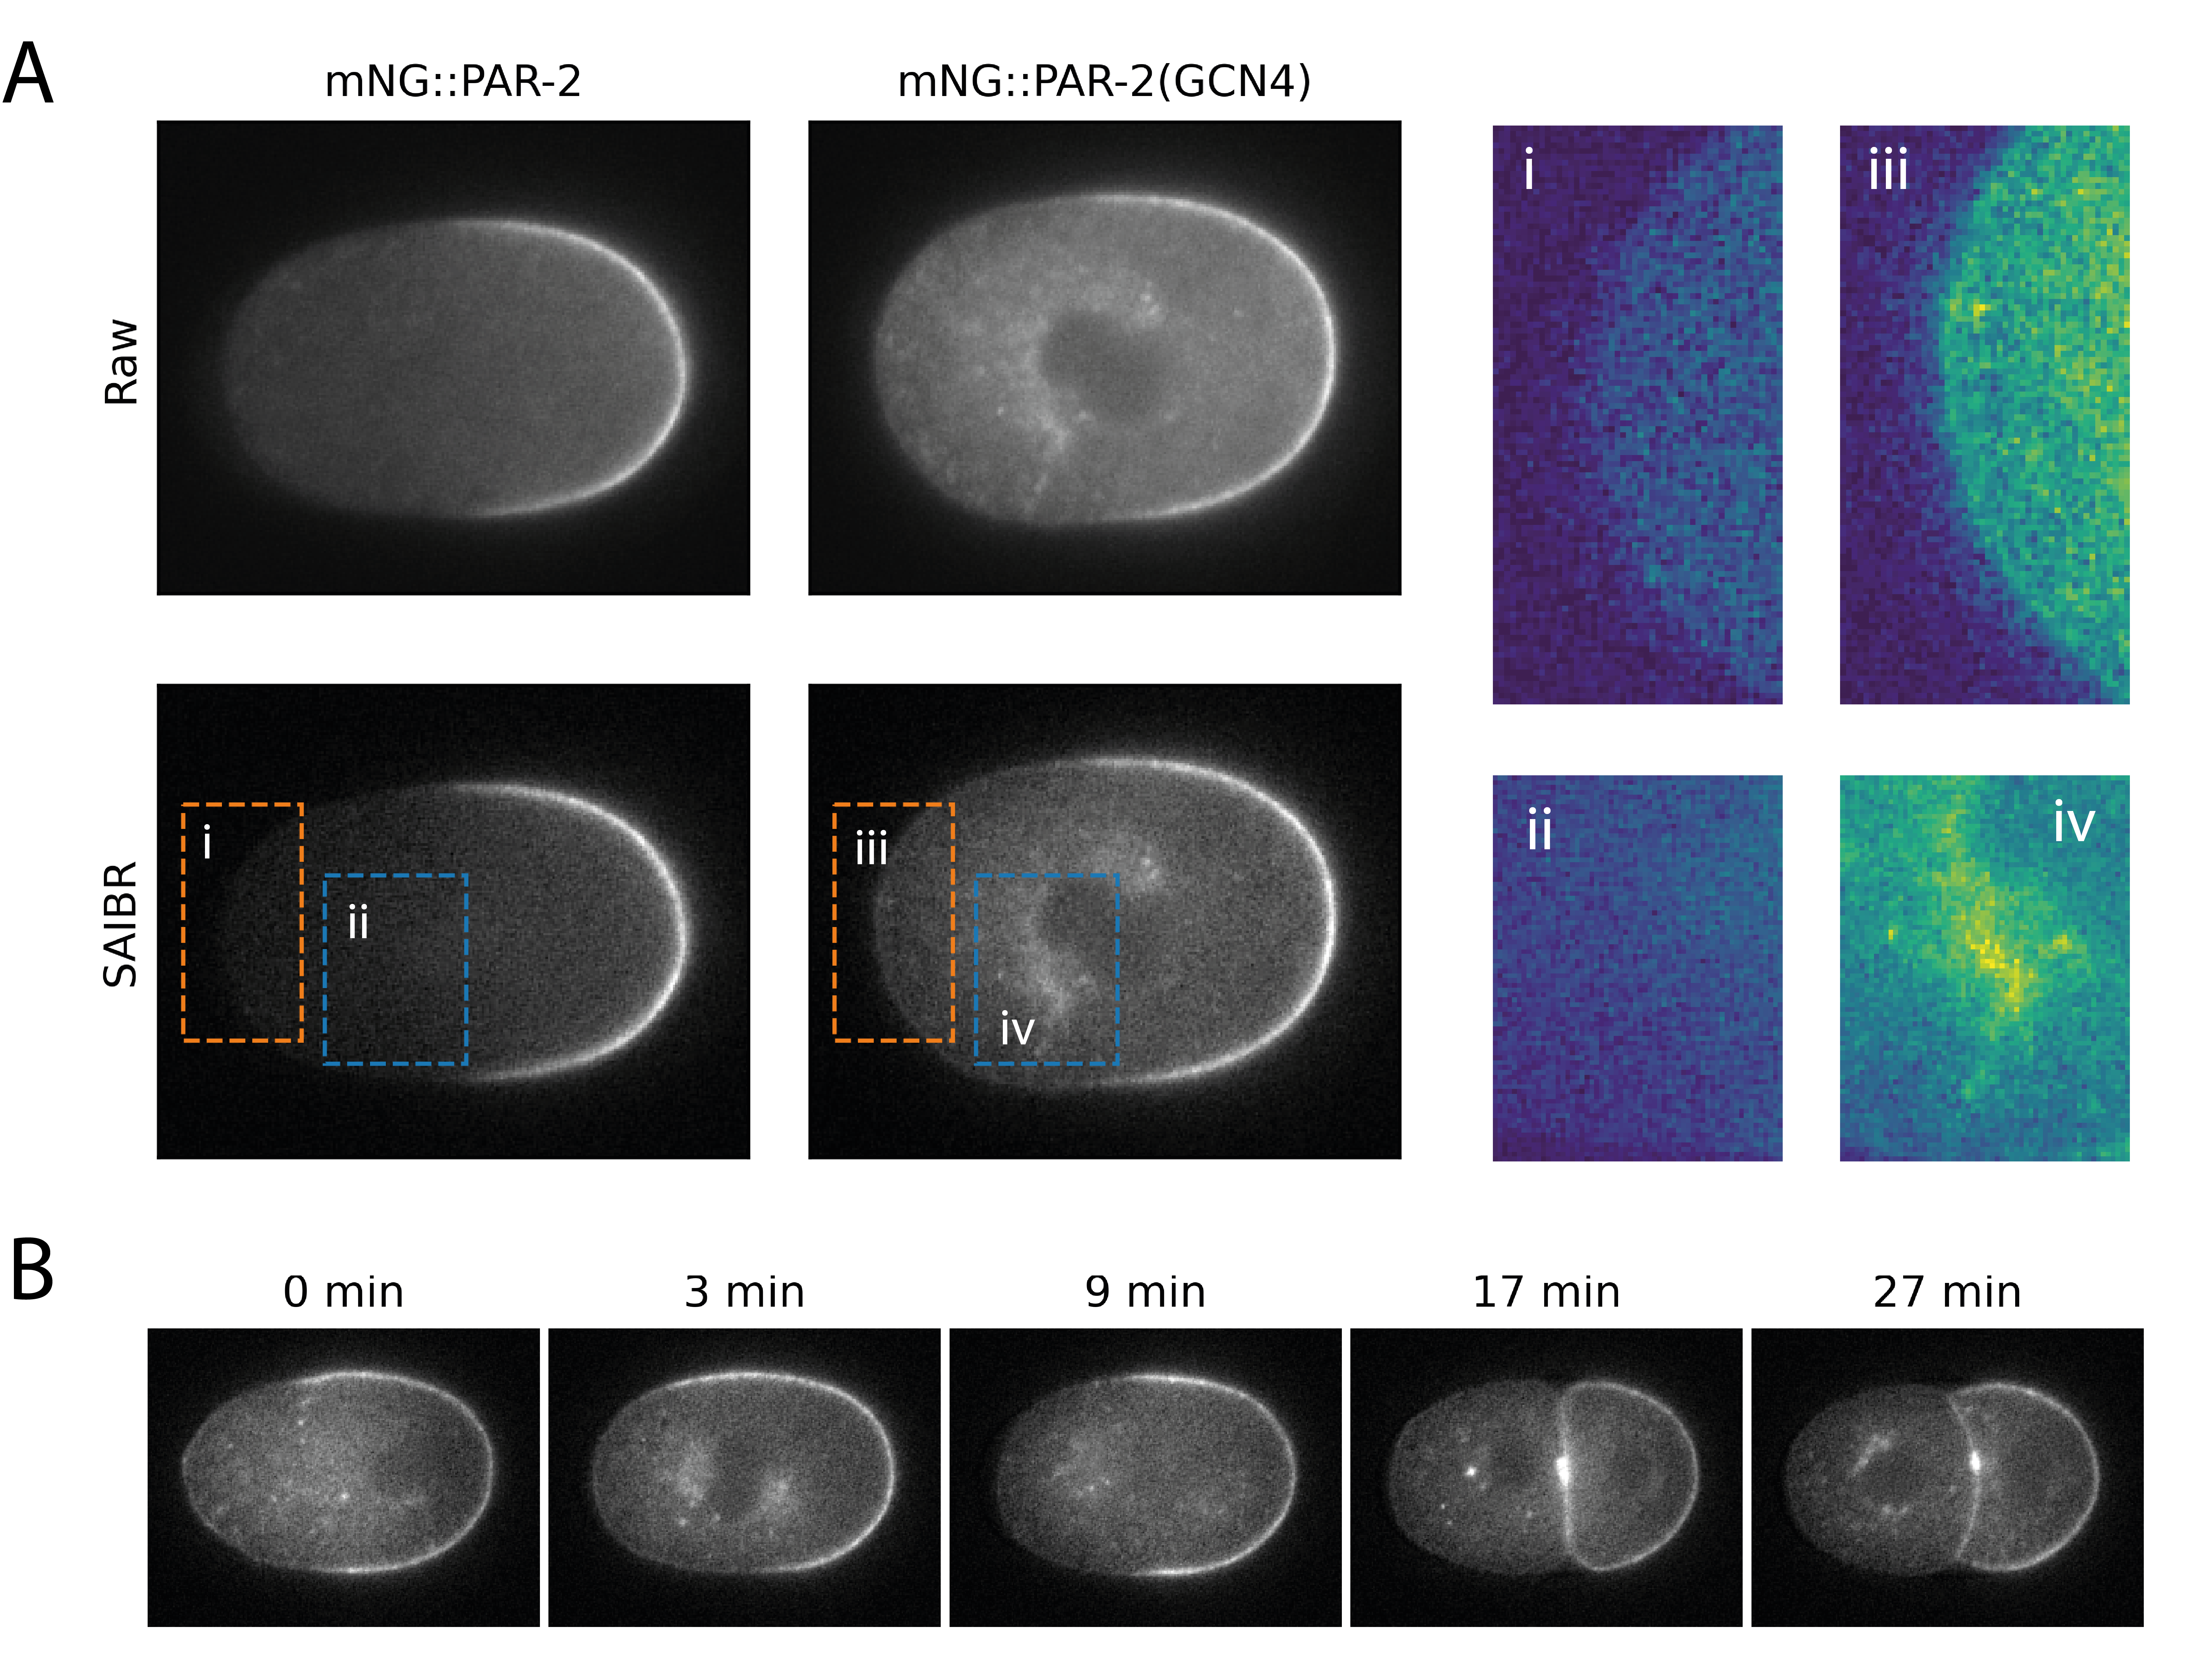
\includegraphics[scale=1]{gcn4}
\setlength{\abovecaptionskip}{20pt}
\centering
\mycaption{Title}{Caption}
\label{fig:gcn4}
\end{figure}

\begin{figure}[!h]
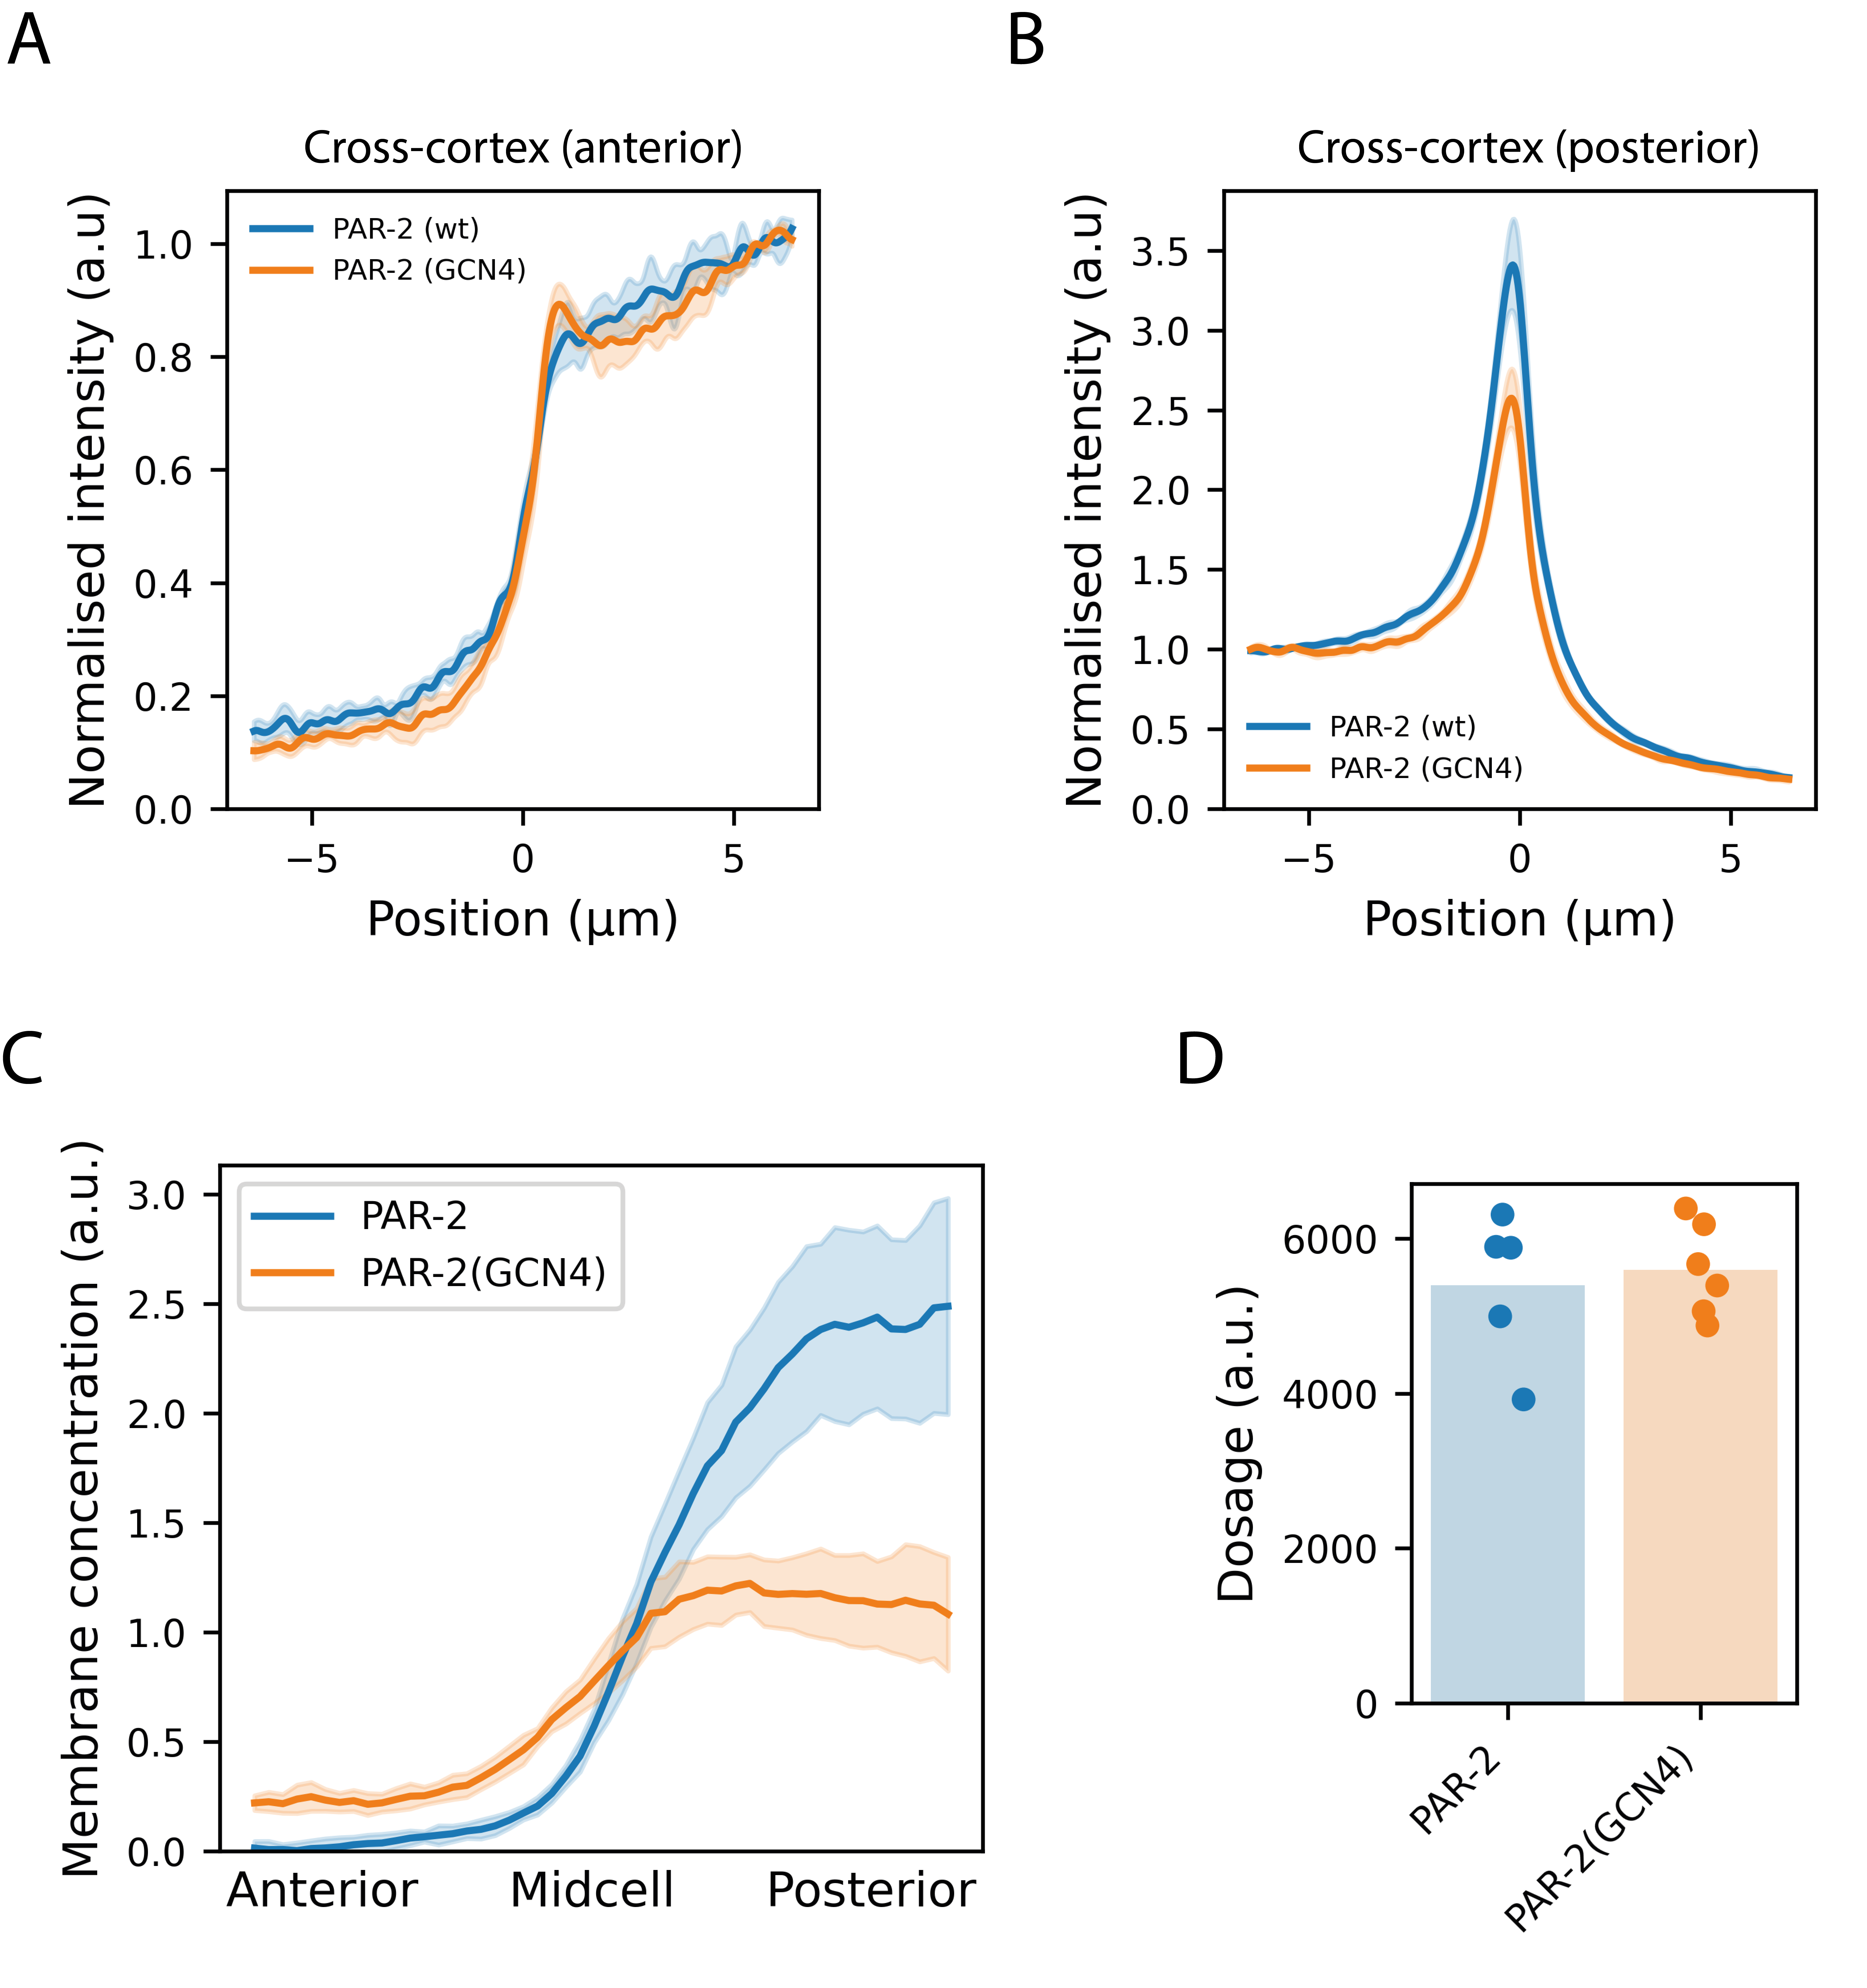
\includegraphics[scale=1]{gcn4_quantification}
\setlength{\abovecaptionskip}{20pt}
\centering
\mycaption{Title}{Caption}
\label{fig:gcn4_quantification}
\end{figure}

\begin{figure}[!h]
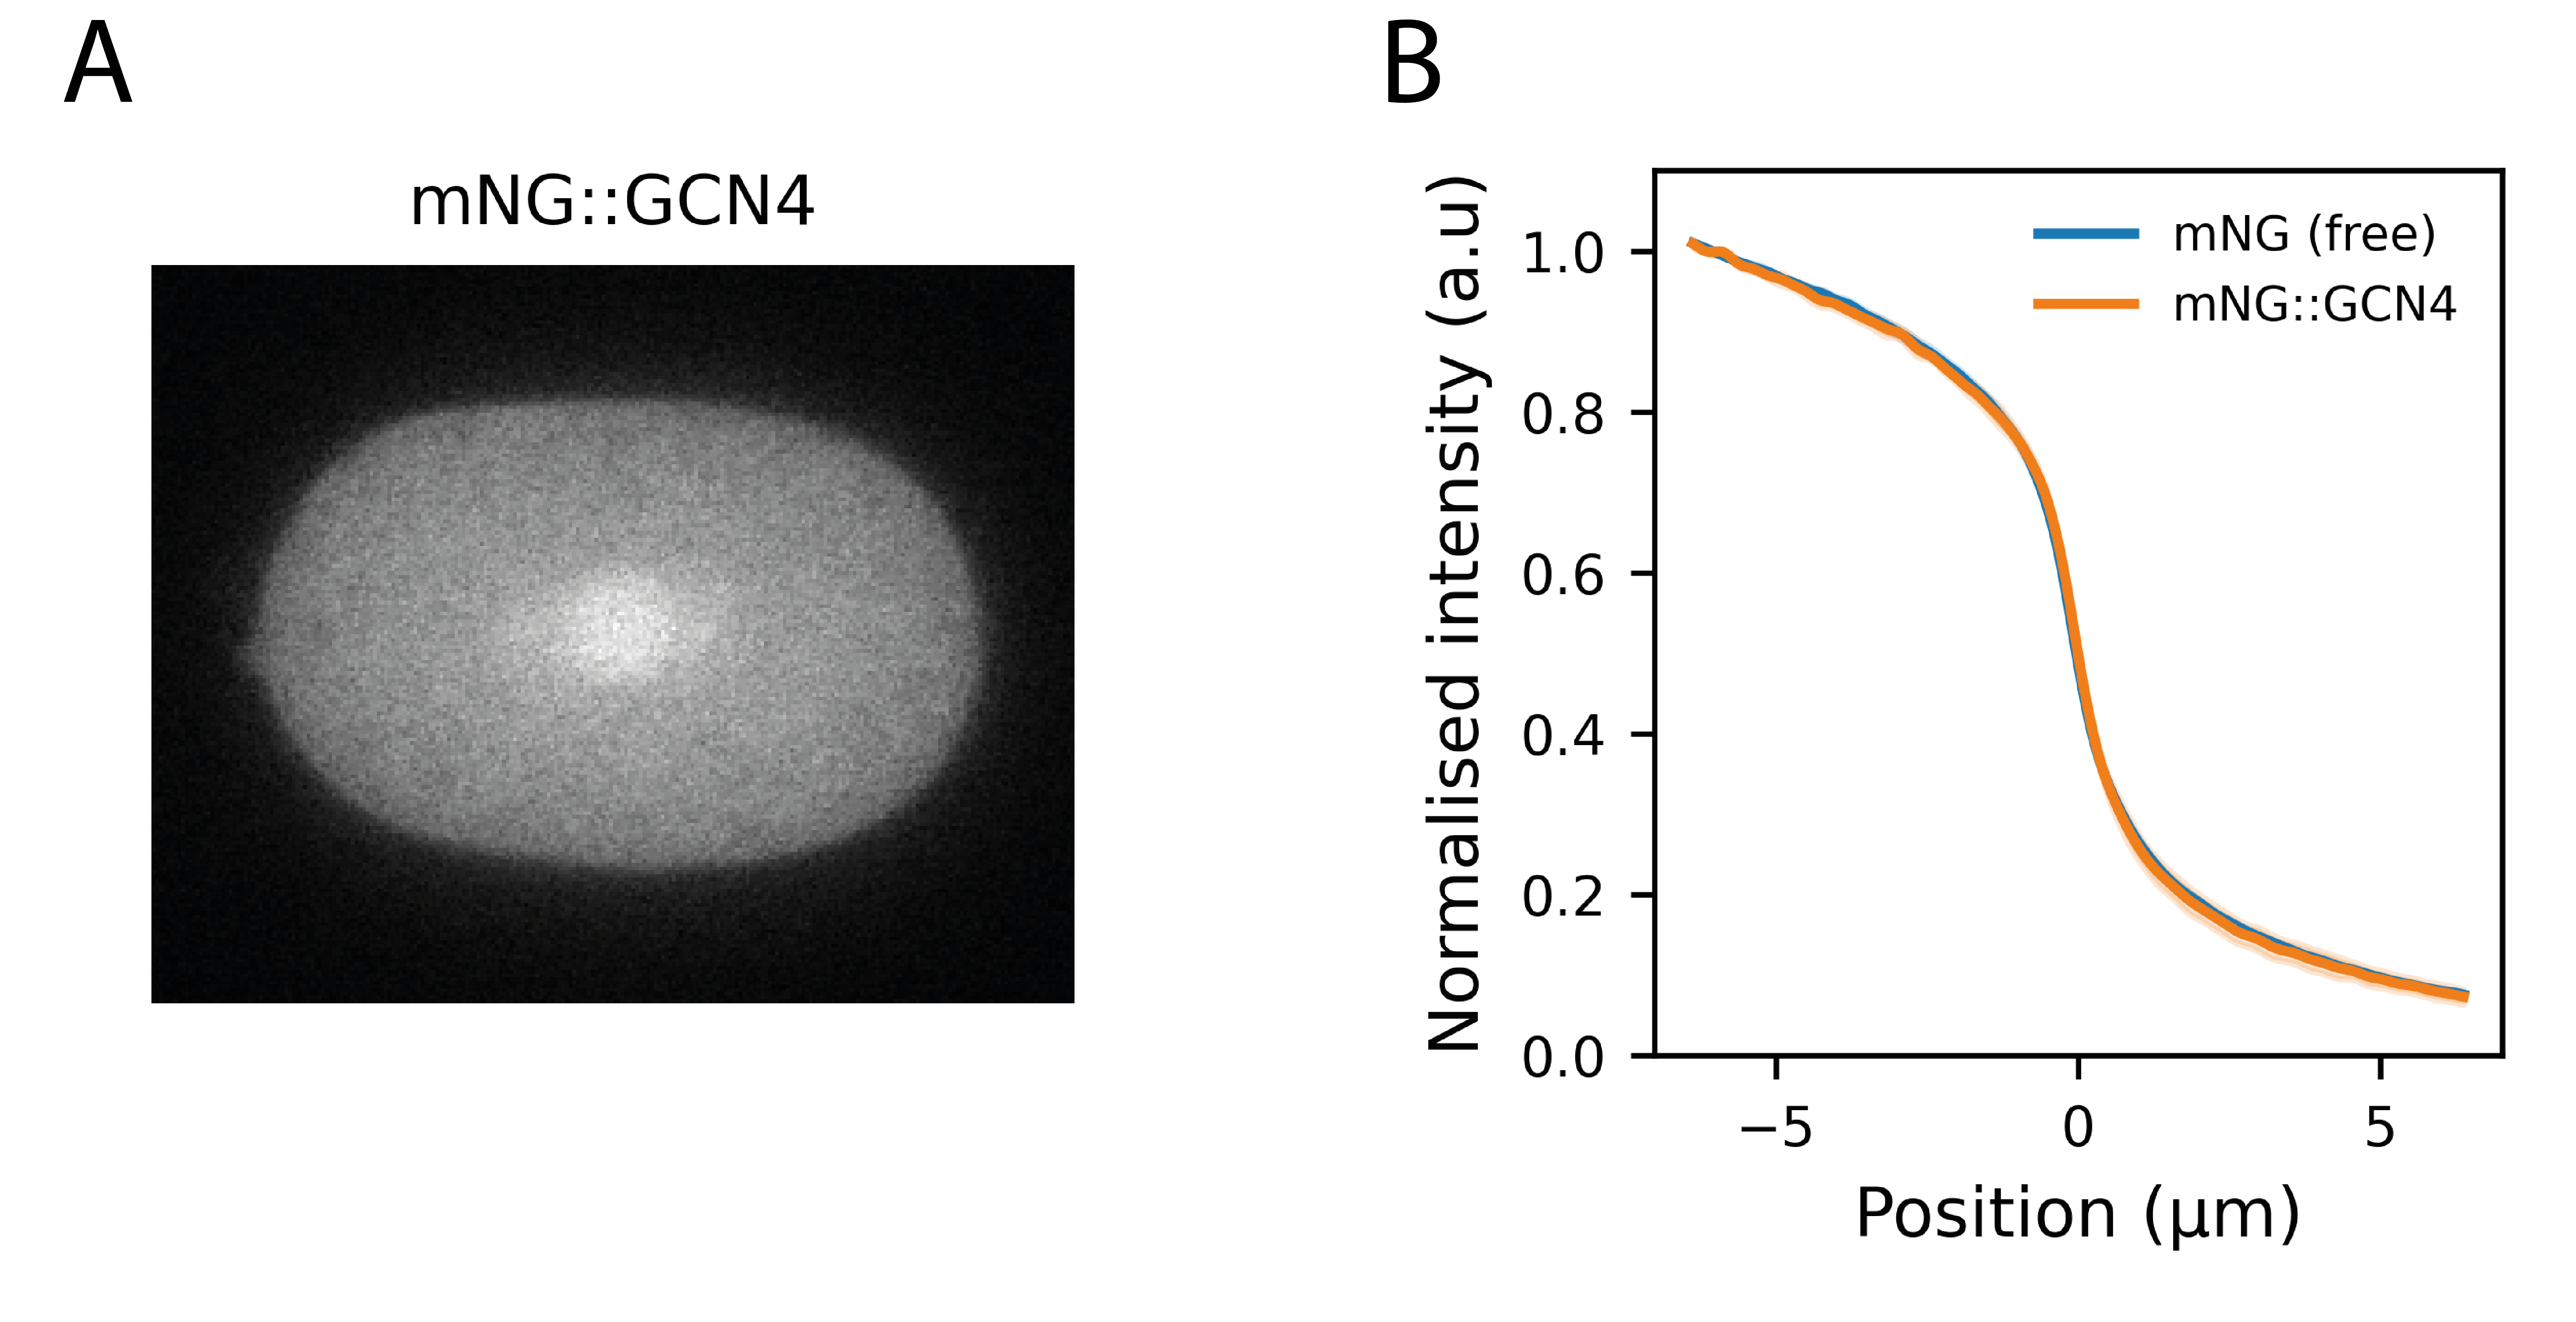
\includegraphics[scale=1]{gcn4_alone}
\setlength{\abovecaptionskip}{20pt}
\centering
\mycaption{Title}{Caption}
\label{fig:gcn4_alone}
\end{figure}

\clearpage
\subsection{Incorporating internal membranes into the thermodynamic model}

I consider two further species, representing monomers and dimers bound to internal membranes.  Concentrations are specified by $\phi_{i,1}$ and $\phi_{i,2}$, chemical potentials $\mu_{i,1}$ and $\mu_{i,2}$ with energy parameters $w_{i,1}$ and $w_{i,2}$, where:

\begin{align}
w_{i,1} &= w_i\\
w_{i,2} &= 2w_i + w_d
\end{align}

where $w_i$ is the internal membrane insertion energy. Thermodynamic equilibrium is reached when:
\begin{equation}
2\mu_{c,1} =  \mu_{c,2} = 2\mu_{p,1} =  \mu_{p,2} = 2\mu_{i,1} =  \mu_{i,2}
\end{equation}

The total amount of protein is conserved according the the following:
\begin{equation}
\overline{\phi} = \phi_c + \alpha\phi_p + \beta\phi_i
\end{equation}

where $\alpha$ is a non-dimensional conversion factor between cytoplasmic and plasma membrane volume fractions, $\beta$ is the equivalent factor for internal membranes. Setting $\overline{\phi}$ as a fixed value, $\phi_{c,1}$, $\phi_{c,2}$, $\phi_{m,1}$, $\phi_{m,2}$, $\phi_{i,1}$ and $\phi_{i,2}$ can be solved numerically. Using this model, we can investigate the relationship between dimerisation energy ($w_d$) and PAR-2 localisation in systems with varying levels of internal membrane charge (varying $w_i$). As shown in fig x, we can see that, in systems where $w_i$ is sufficiently high, constitutive dimerisation (high $w_d$) can result in considerable PAR-2 levels on internal membranes, which isn't observed at lower/intermediate dimerisation strengths. 

\begin{figure}[!h]
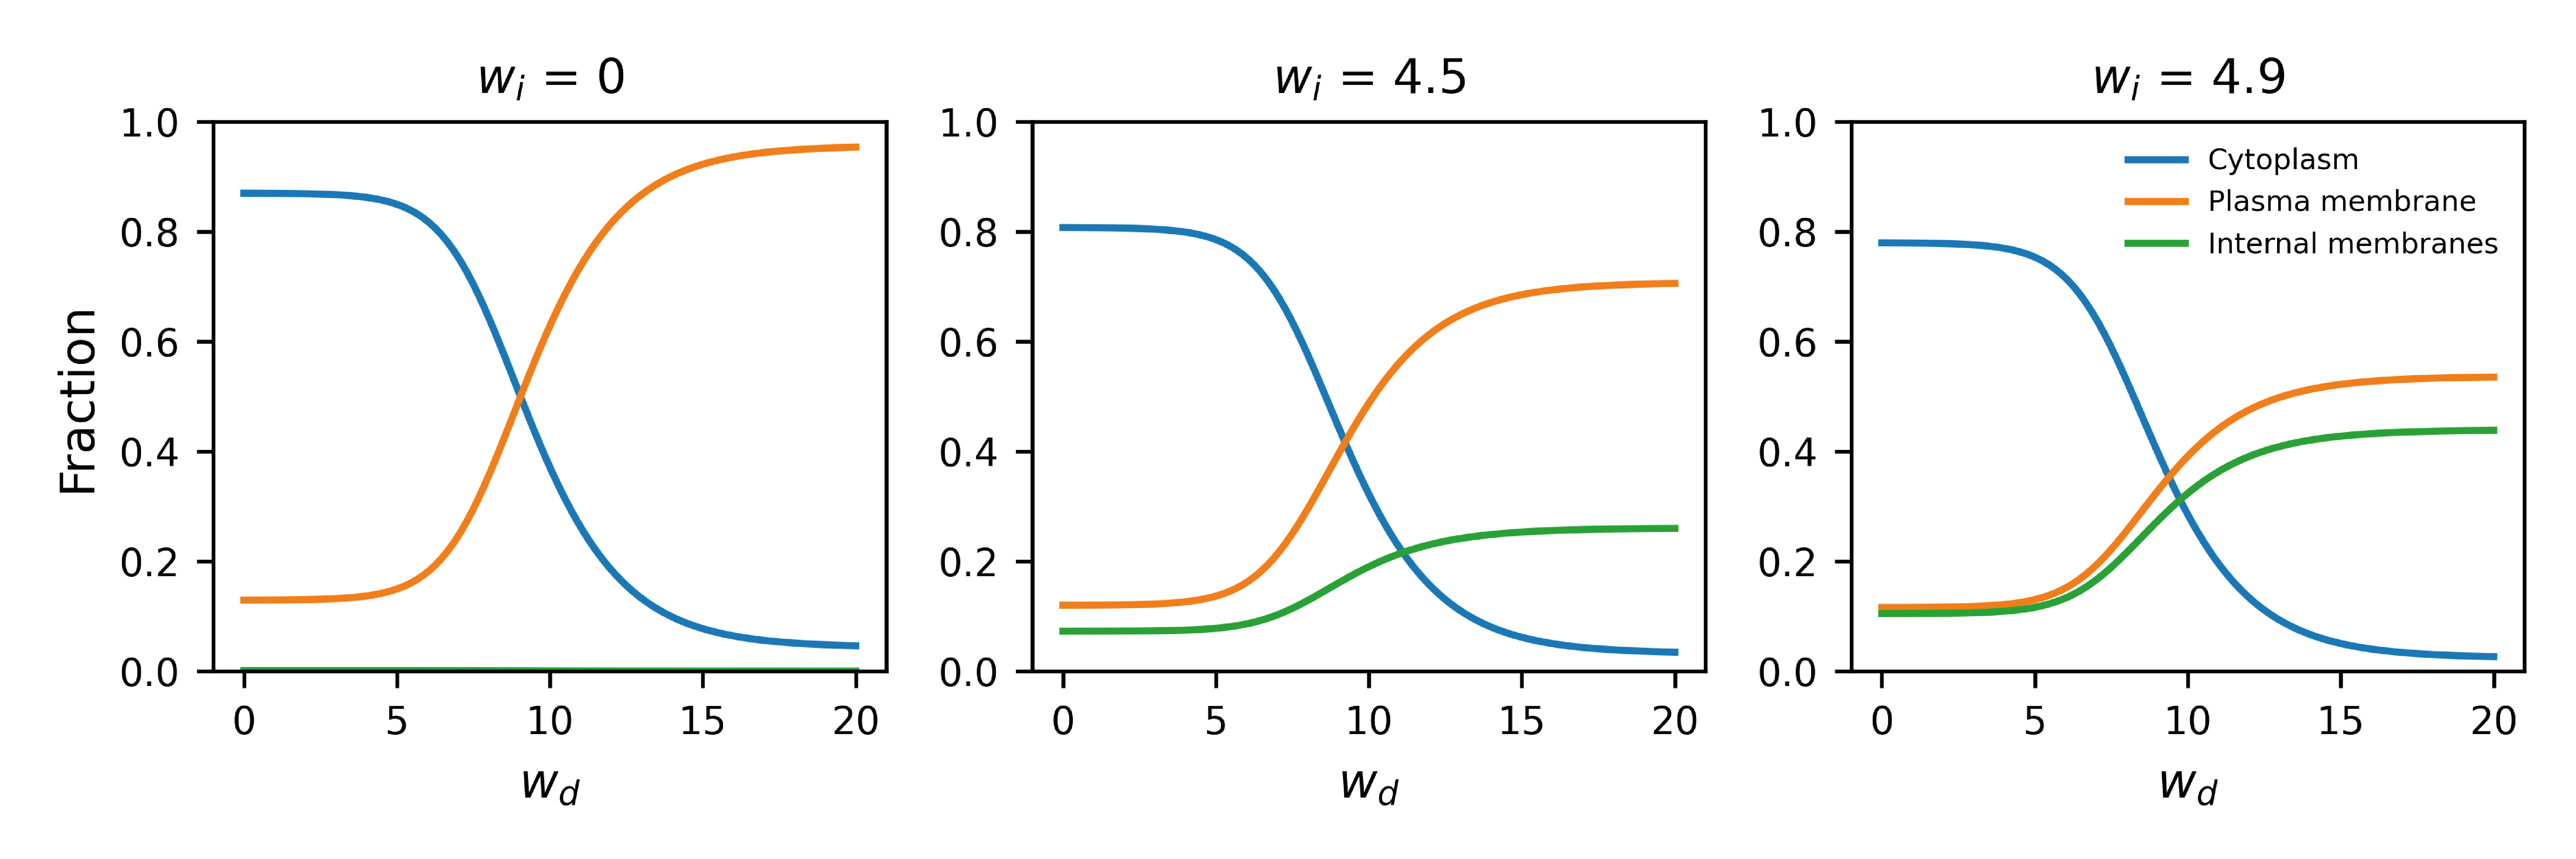
\includegraphics[scale=0.90]{six_species_thermodynamic}
\setlength{\abovecaptionskip}{20pt}
\centering
\mycaption{Title}{Caption}
\label{fig:six_species_thermodynamic}
\end{figure}

% Whilst increasing wd may increase binding to internal membranes (provided that wi is high enough), this should always be accompanied by an increase in levels at the plasma membrane. In other words, we cannot get a scenario akin to what we see in vivo,  whereby constitutive dimerisation actually reduces levels on the plasma membrane.


\subsection{Consideration of membrane exchange kinetics}


\begin{figure}[!h]
\includegraphics[scale=0.95]{three_surface_kinetic}
\setlength{\abovecaptionskip}{20pt}
\centering
\mycaption{Title}{Caption}
\label{fig:three_surface_kinetic}
\end{figure}


\subsection{Monitoring the system closer to equilibrium in vivo}

\begin{figure}[!h]
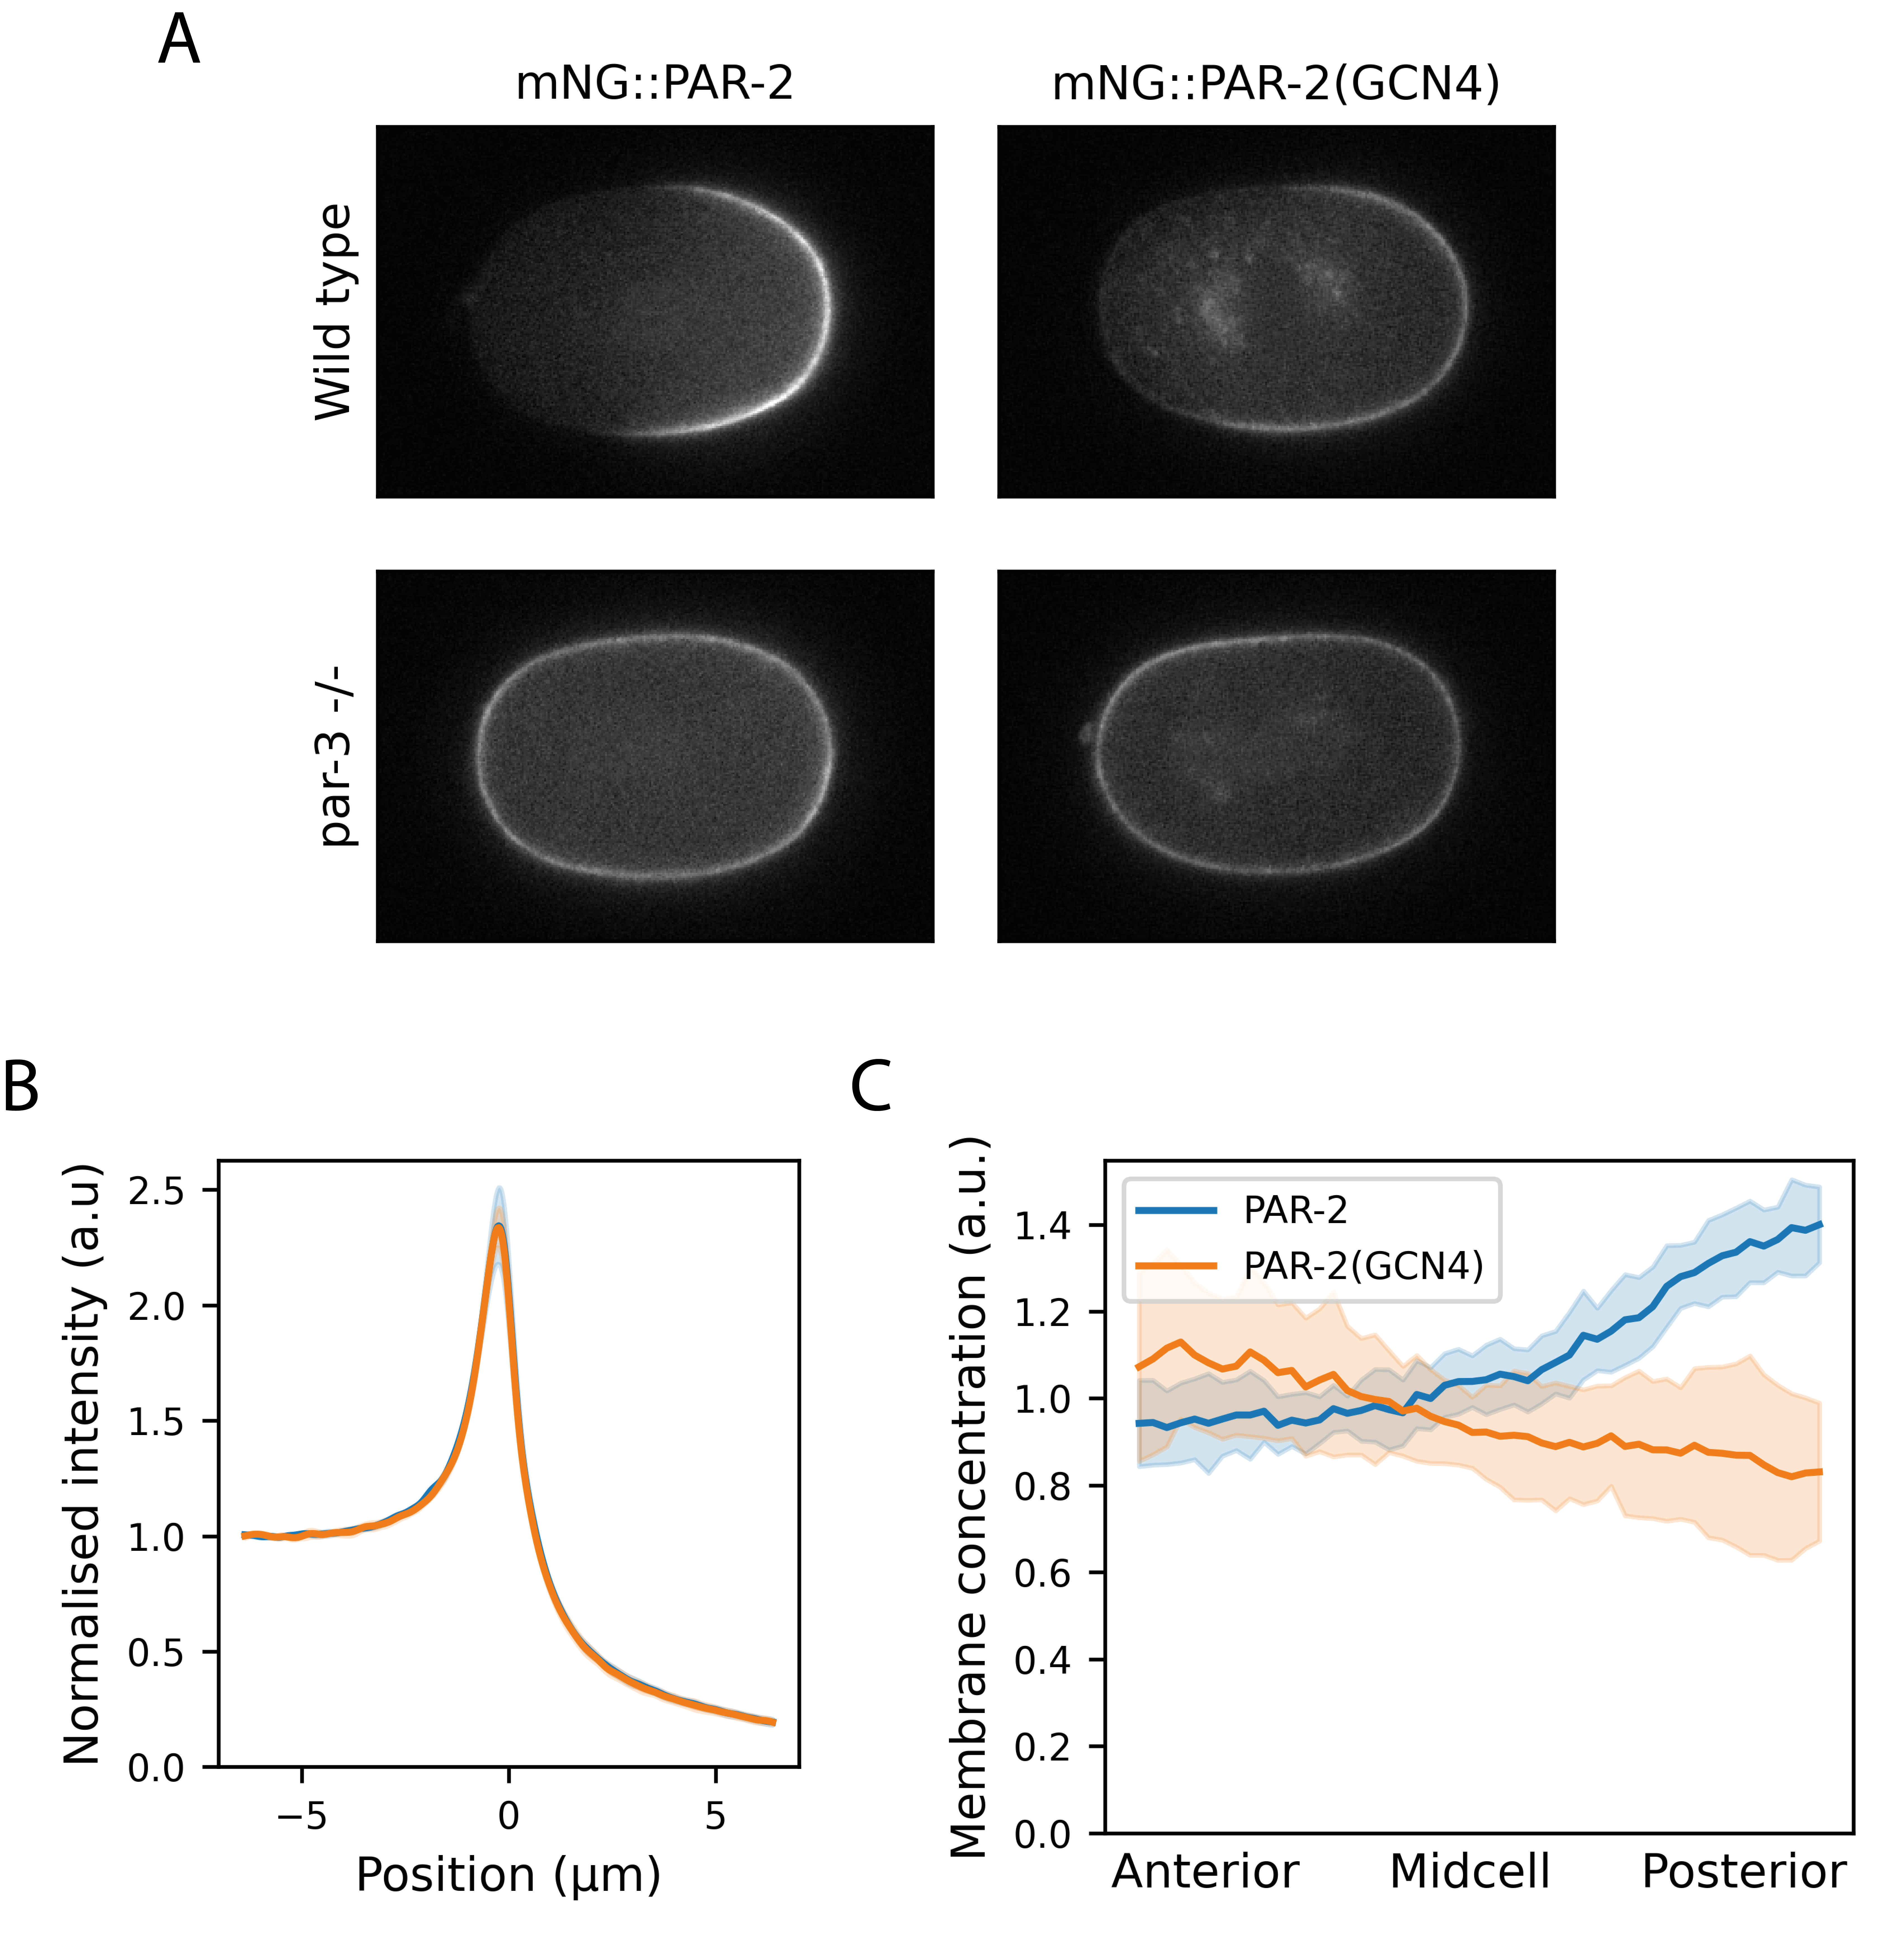
\includegraphics[scale=0.95]{gcn4_par3mut}
\setlength{\abovecaptionskip}{20pt}
\centering
\mycaption{Title}{Caption}
\label{fig:gcn4_par3mut}
\end{figure}




%%%%%%%%%%%%%%%%%%%%%%%%%%%%%%%%%%%%%%%%%%%%%%%%%%%%%%%%%%
\clearpage
\section{Discussion}


%%%%%%%%%%%%%%%%%%%%%%%%%%%%%%%%%%%%%%%%%%%%%%%%%%%%%%%%%%
\clearpage
\section{Materials and methods}


\subsection{Worm maintenance}
\subsection{Generating transgenic lines by CRISPR}

\begin{figure}[!h]
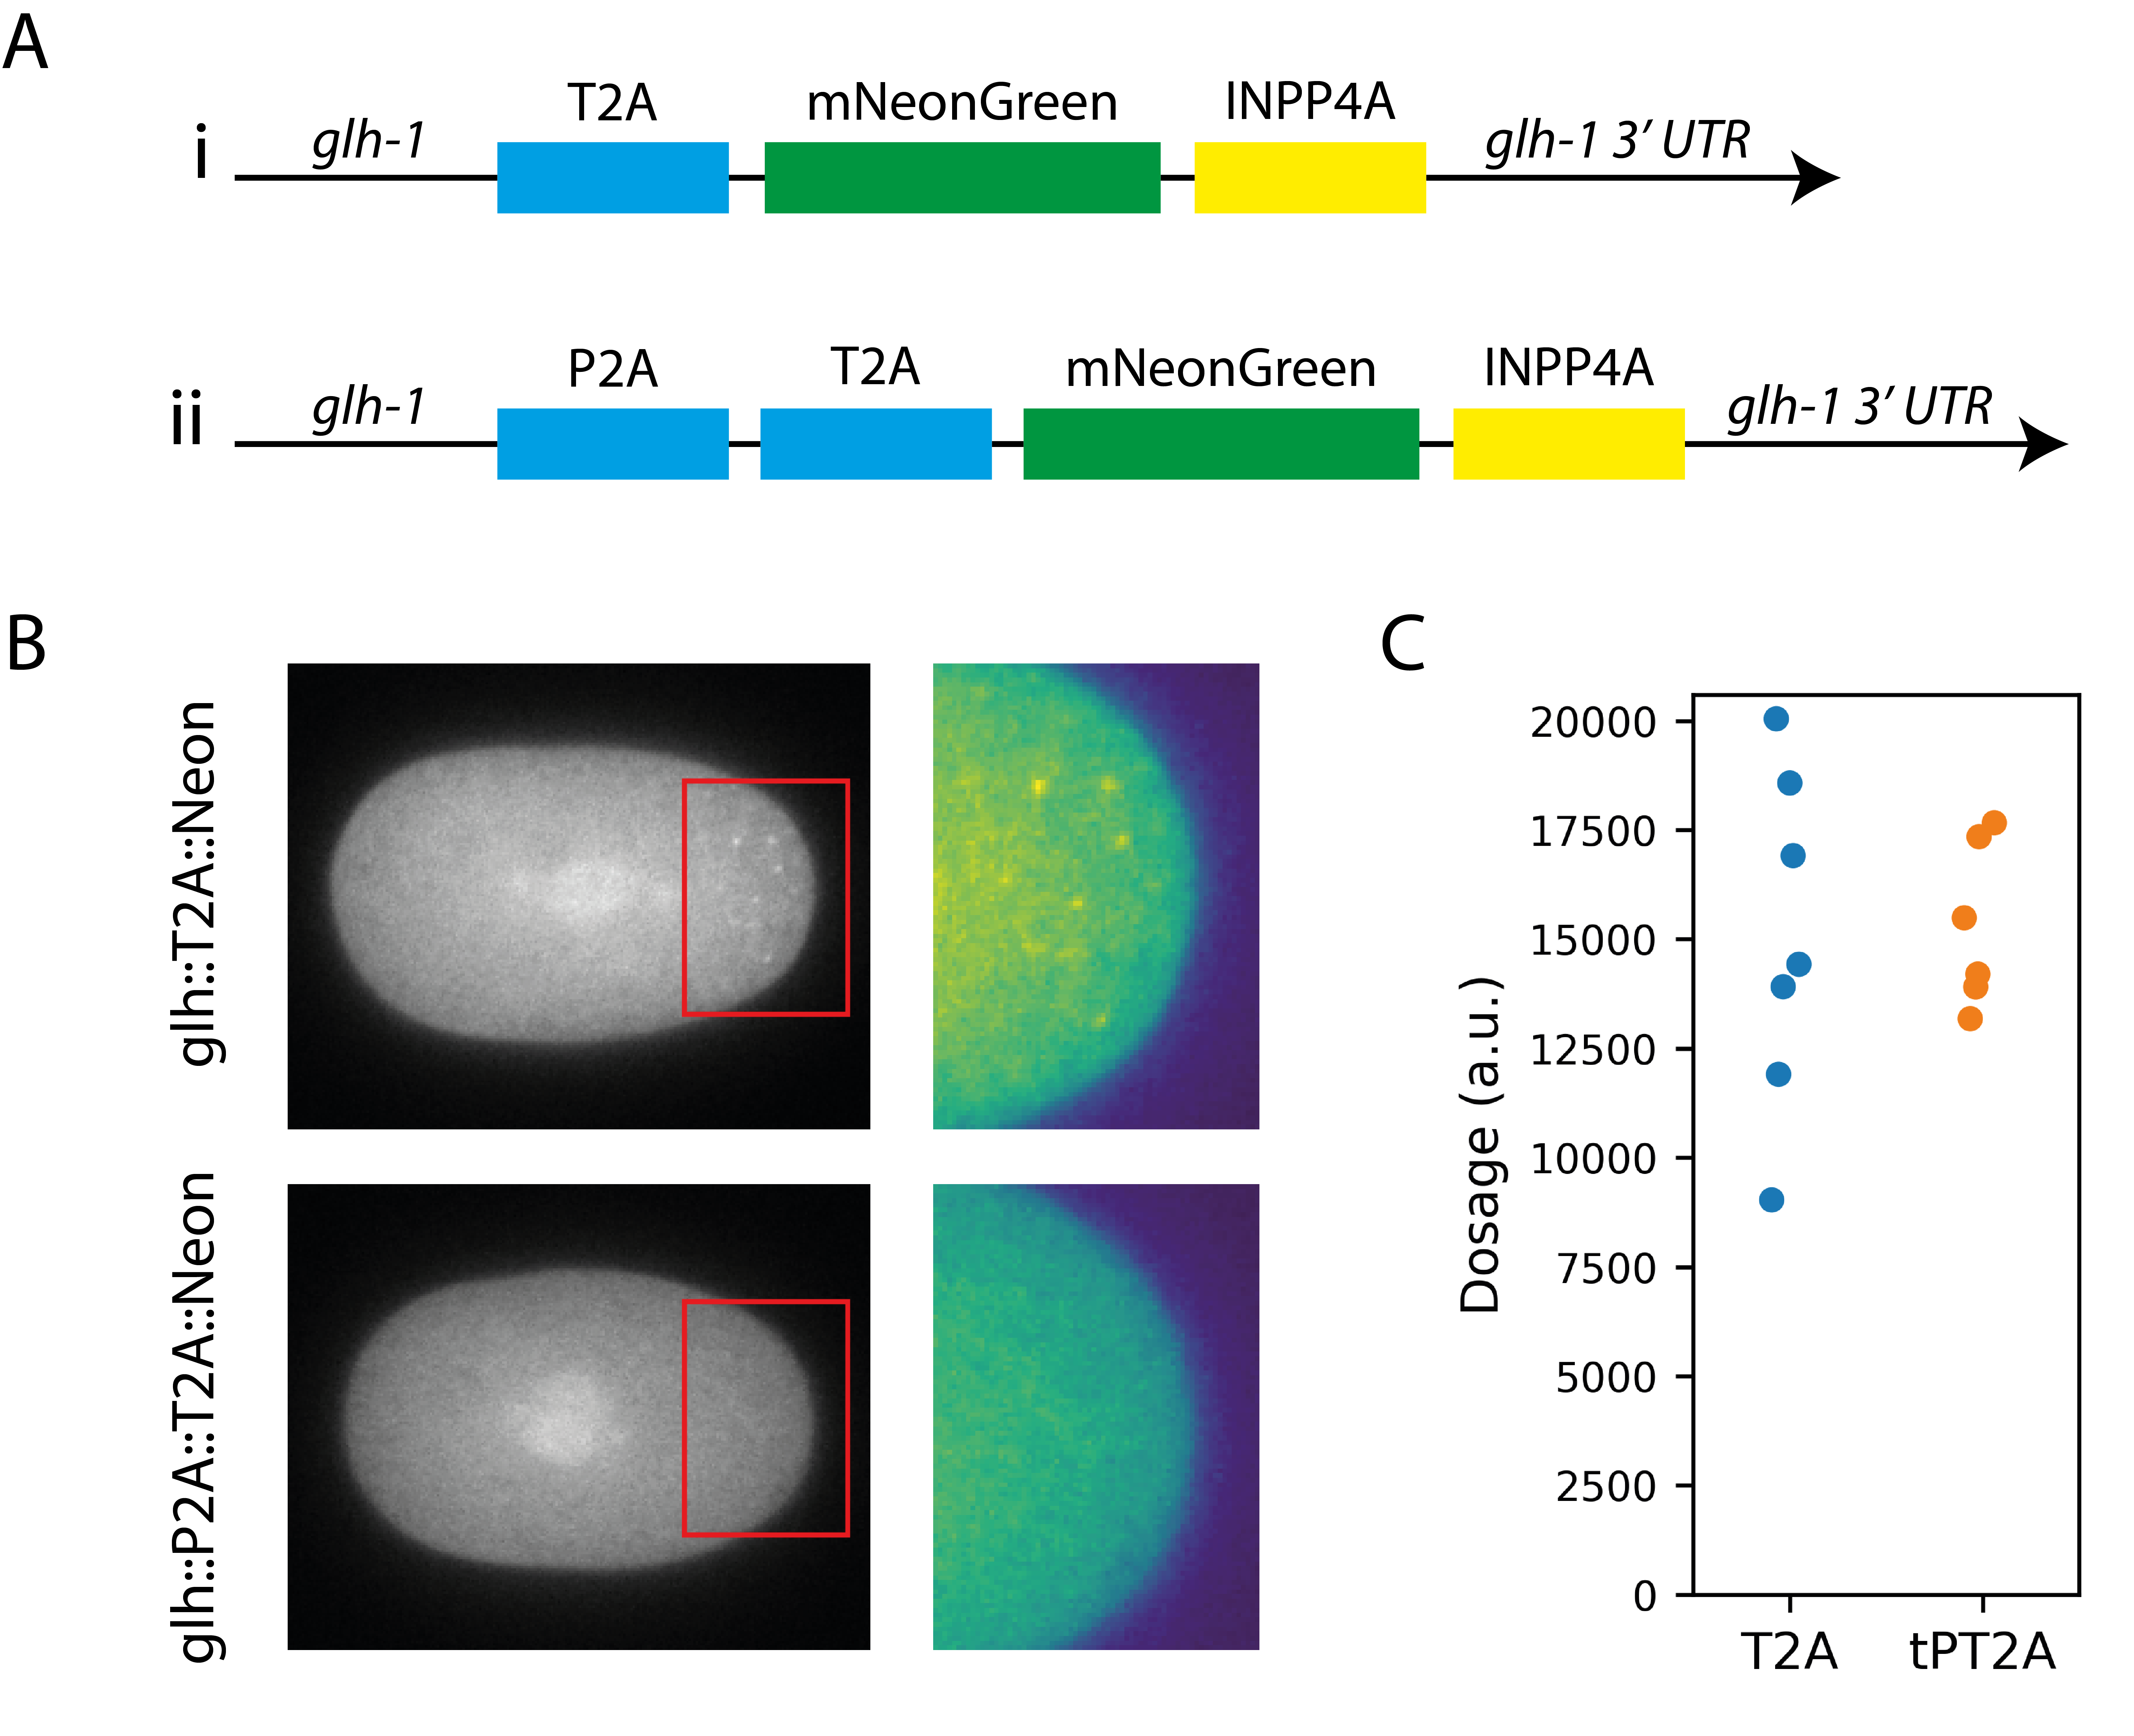
\includegraphics[scale=1]{glh}
\setlength{\abovecaptionskip}{20pt}
\centering
\mycaption{Title}{Caption}
\label{fig:glh}
\end{figure}



\subsection{Microscopy}
\subsection{Full-length PAR-2 purification}
\subsection{Ubiquitination assays}
\subsection{PAR-2 RING domain fragment purification}
\subsection{SEC-MALS}
\subsection{Image analysis}
\subsection{Modelling methods}

%%%%%%%%%%%%%%%%%%%%%%%%%%%%%%%%%%%%%%%%%%%%%%%%%%%%%%%%%%
\clearpage
\section{Appendix: Analysis of PAR-2 diffusion kinetics by single particle tracking}


%%%%%%%%%%%%%%%%%%%%%%%%%%%%%%%%%%%%%%%%%%%%%%%%%%%%%%%%%%
\clearpage
\section{Bibliography}

\printbibliography

\end{document}
